% Options for packages loaded elsewhere
\PassOptionsToPackage{unicode}{hyperref}
\PassOptionsToPackage{hyphens}{url}
%
\documentclass[
]{book}
\usepackage{amsmath,amssymb}
\usepackage{iftex}
\ifPDFTeX
  \usepackage[T1]{fontenc}
  \usepackage[utf8]{inputenc}
  \usepackage{textcomp} % provide euro and other symbols
\else % if luatex or xetex
  \usepackage{unicode-math} % this also loads fontspec
  \defaultfontfeatures{Scale=MatchLowercase}
  \defaultfontfeatures[\rmfamily]{Ligatures=TeX,Scale=1}
\fi
\usepackage{lmodern}
\ifPDFTeX\else
  % xetex/luatex font selection
\fi
% Use upquote if available, for straight quotes in verbatim environments
\IfFileExists{upquote.sty}{\usepackage{upquote}}{}
\IfFileExists{microtype.sty}{% use microtype if available
  \usepackage[]{microtype}
  \UseMicrotypeSet[protrusion]{basicmath} % disable protrusion for tt fonts
}{}
\makeatletter
\@ifundefined{KOMAClassName}{% if non-KOMA class
  \IfFileExists{parskip.sty}{%
    \usepackage{parskip}
  }{% else
    \setlength{\parindent}{0pt}
    \setlength{\parskip}{6pt plus 2pt minus 1pt}}
}{% if KOMA class
  \KOMAoptions{parskip=half}}
\makeatother
\usepackage{xcolor}
\usepackage{color}
\usepackage{fancyvrb}
\newcommand{\VerbBar}{|}
\newcommand{\VERB}{\Verb[commandchars=\\\{\}]}
\DefineVerbatimEnvironment{Highlighting}{Verbatim}{commandchars=\\\{\}}
% Add ',fontsize=\small' for more characters per line
\usepackage{framed}
\definecolor{shadecolor}{RGB}{248,248,248}
\newenvironment{Shaded}{\begin{snugshade}}{\end{snugshade}}
\newcommand{\AlertTok}[1]{\textcolor[rgb]{0.94,0.16,0.16}{#1}}
\newcommand{\AnnotationTok}[1]{\textcolor[rgb]{0.56,0.35,0.01}{\textbf{\textit{#1}}}}
\newcommand{\AttributeTok}[1]{\textcolor[rgb]{0.13,0.29,0.53}{#1}}
\newcommand{\BaseNTok}[1]{\textcolor[rgb]{0.00,0.00,0.81}{#1}}
\newcommand{\BuiltInTok}[1]{#1}
\newcommand{\CharTok}[1]{\textcolor[rgb]{0.31,0.60,0.02}{#1}}
\newcommand{\CommentTok}[1]{\textcolor[rgb]{0.56,0.35,0.01}{\textit{#1}}}
\newcommand{\CommentVarTok}[1]{\textcolor[rgb]{0.56,0.35,0.01}{\textbf{\textit{#1}}}}
\newcommand{\ConstantTok}[1]{\textcolor[rgb]{0.56,0.35,0.01}{#1}}
\newcommand{\ControlFlowTok}[1]{\textcolor[rgb]{0.13,0.29,0.53}{\textbf{#1}}}
\newcommand{\DataTypeTok}[1]{\textcolor[rgb]{0.13,0.29,0.53}{#1}}
\newcommand{\DecValTok}[1]{\textcolor[rgb]{0.00,0.00,0.81}{#1}}
\newcommand{\DocumentationTok}[1]{\textcolor[rgb]{0.56,0.35,0.01}{\textbf{\textit{#1}}}}
\newcommand{\ErrorTok}[1]{\textcolor[rgb]{0.64,0.00,0.00}{\textbf{#1}}}
\newcommand{\ExtensionTok}[1]{#1}
\newcommand{\FloatTok}[1]{\textcolor[rgb]{0.00,0.00,0.81}{#1}}
\newcommand{\FunctionTok}[1]{\textcolor[rgb]{0.13,0.29,0.53}{\textbf{#1}}}
\newcommand{\ImportTok}[1]{#1}
\newcommand{\InformationTok}[1]{\textcolor[rgb]{0.56,0.35,0.01}{\textbf{\textit{#1}}}}
\newcommand{\KeywordTok}[1]{\textcolor[rgb]{0.13,0.29,0.53}{\textbf{#1}}}
\newcommand{\NormalTok}[1]{#1}
\newcommand{\OperatorTok}[1]{\textcolor[rgb]{0.81,0.36,0.00}{\textbf{#1}}}
\newcommand{\OtherTok}[1]{\textcolor[rgb]{0.56,0.35,0.01}{#1}}
\newcommand{\PreprocessorTok}[1]{\textcolor[rgb]{0.56,0.35,0.01}{\textit{#1}}}
\newcommand{\RegionMarkerTok}[1]{#1}
\newcommand{\SpecialCharTok}[1]{\textcolor[rgb]{0.81,0.36,0.00}{\textbf{#1}}}
\newcommand{\SpecialStringTok}[1]{\textcolor[rgb]{0.31,0.60,0.02}{#1}}
\newcommand{\StringTok}[1]{\textcolor[rgb]{0.31,0.60,0.02}{#1}}
\newcommand{\VariableTok}[1]{\textcolor[rgb]{0.00,0.00,0.00}{#1}}
\newcommand{\VerbatimStringTok}[1]{\textcolor[rgb]{0.31,0.60,0.02}{#1}}
\newcommand{\WarningTok}[1]{\textcolor[rgb]{0.56,0.35,0.01}{\textbf{\textit{#1}}}}
\usepackage{longtable,booktabs,array}
\usepackage{calc} % for calculating minipage widths
% Correct order of tables after \paragraph or \subparagraph
\usepackage{etoolbox}
\makeatletter
\patchcmd\longtable{\par}{\if@noskipsec\mbox{}\fi\par}{}{}
\makeatother
% Allow footnotes in longtable head/foot
\IfFileExists{footnotehyper.sty}{\usepackage{footnotehyper}}{\usepackage{footnote}}
\makesavenoteenv{longtable}
\usepackage{graphicx}
\makeatletter
\def\maxwidth{\ifdim\Gin@nat@width>\linewidth\linewidth\else\Gin@nat@width\fi}
\def\maxheight{\ifdim\Gin@nat@height>\textheight\textheight\else\Gin@nat@height\fi}
\makeatother
% Scale images if necessary, so that they will not overflow the page
% margins by default, and it is still possible to overwrite the defaults
% using explicit options in \includegraphics[width, height, ...]{}
\setkeys{Gin}{width=\maxwidth,height=\maxheight,keepaspectratio}
% Set default figure placement to htbp
\makeatletter
\def\fps@figure{htbp}
\makeatother
\setlength{\emergencystretch}{3em} % prevent overfull lines
\providecommand{\tightlist}{%
  \setlength{\itemsep}{0pt}\setlength{\parskip}{0pt}}
\setcounter{secnumdepth}{5}
\usepackage{booktabs}


\ifLuaTeX
  \usepackage{selnolig}  % disable illegal ligatures
\fi
\usepackage[]{natbib}
\bibliographystyle{apalike}
\IfFileExists{bookmark.sty}{\usepackage{bookmark}}{\usepackage{hyperref}}
\IfFileExists{xurl.sty}{\usepackage{xurl}}{} % add URL line breaks if available
\urlstyle{same}
\hypersetup{
  pdftitle={Foundations of Statistics},
  pdfauthor={Prof Peter Neal and Dr Daniel Cavey},
  hidelinks,
  pdfcreator={LaTeX via pandoc}}

\title{Foundations of Statistics}
\author{Prof Peter Neal and Dr Daniel Cavey}
\date{Autumn Semester 2023, University of Nottingham}

\begin{document}
\maketitle

{
\setcounter{tocdepth}{1}
\tableofcontents
}
\hypertarget{preliminaries}{%
\chapter*{Preliminaries}\label{preliminaries}}
\addcontentsline{toc}{chapter}{Preliminaries}

\hypertarget{overview}{%
\section*{Overview}\label{overview}}
\addcontentsline{toc}{section}{Overview}

In this course the fundamental principles and techniques underlying modern statistical and data analysis will be introduced. The course will cover the core foundations of statistical theory consisting of:

\begin{itemize}
\tightlist
\item
  probability distributions and techniques;\\
\item
  statistical concepts and methods;\\
\item
  linear models.
\end{itemize}

The course highlights the importance of computers, and in particular, statistical packages, in performing modern statistical analysis. Students will be introduced to the statistical package \textbf{R} as a statistical and programming tool and will gain experience in interpreting and communicating its output.

\textbf{Learning Outcomes}

A student who completes this module successfully will be able to:

\begin{itemize}
\tightlist
\item
  derive and explain properties of basic statistical inference; linear regression models and probability techniques;\\
\item
  perform exploratory data analysis; summarising their analysis and proposing further investigations;\\
\item
  derive point and interval estimators, and perform hypothesis tests for a variety of situations;\\
\item
  apply the theory and methods for statistical inference, linear regression models and probability techniques to a wide range of practical examples;\\
\item
  use the statistical package \textbf{R} to derive results concerning statistical inference;\\
\item
  communicate their statistical analysis in a written report.
\end{itemize}

\textbf{Syllabus Overview}

\begin{itemize}
\tightlist
\item
  Summary statistics and visualising data\\
\item
  Probability, random variables and expectation\\
\item
  Joint distributions, conditional distribution, covariance and correlation\\
\item
  Central limit theorem\\
\item
  Parameter estimation - Method of Moments and Maximum Likelihood Estimation\\
\item
  Transformations of random variables\\
\item
  Multivariate normal distribution\\
\item
  Linear Models\\
\item
  Least squares estimation\\
\item
  Interval estimation\\
\item
  Hypothesis testing and goodness-of-fit\\
\item
  ANOVA
\end{itemize}

\hypertarget{tasks}{%
\section*{Tasks}\label{tasks}}
\addcontentsline{toc}{section}{Tasks}

At the end of most chapters there are tasks to complete. These tasks will either be computer lab sessions using the statistical package \textbf{R} or statistical exercises or both to reinforce the material covered in the chapter (or the last couple of chapters).

\hypertarget{intro}{%
\chapter{Introduction}\label{intro}}

\hypertarget{intro_stats}{%
\section{What is Statistics?}\label{intro_stats}}

Watch \href{https://mediaspace.nottingham.ac.uk/media/What+is+Statistics+FINAL+VERSION/1_uu88cciu}{\textcolor{blue}{Video 1: What is Statistics?}}

\textbf{Statistics} is the field of mathematics concerned with reasoning about data and uncertainty.

This includes collecting, organising, summarising, analysing and presenting data.

In particular, Statistics provides the tools for making decisions and drawing conclusions from data in a principled way---this is called \textbf{statistical inference}.

A key part of statistics is \textbf{communicating}: communicating context, data, assumptions, analysis, results.

\hypertarget{intro_population}{%
\section{Populations and samples}\label{intro_population}}

A key idea in Statistics is to draw conclusions about a \textbf{population} based
on a \textbf{sample} from that population. This is where the word \emph{inference} comes from:
we are \emph{inferring} something about the population based on the sample.

\leavevmode\vadjust pre{\hypertarget{des:population}{}}%
{\textbf{Population}}\\
A \textbf{population} is a group or collection of similar individuals (\emph{e.g.~students}), items (\emph{e.g.~plants}) or events (\emph{e.g.~days}) that are of interest to us.

When we want to make inferences about a population, it would be very
time consuming and expensive to look at every member of the population. It could also be destructive if the experiment involves testing until failure.

\leavevmode\vadjust pre{\hypertarget{des:sample}{}}%
{\textbf{Sample}}\\
A \textbf{sample} is a subset of the population.

\begin{figure}
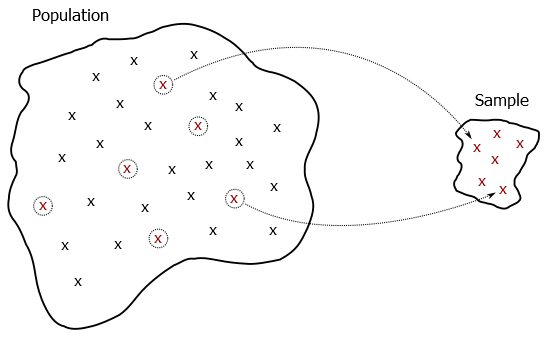
\includegraphics[width=0.65\linewidth]{_main_files/figure-latex/figSvg-1} \caption{A sample is a subset of the population. Each x here represents a sampling unit; red shows the ones in the sample.}\label{fig:figSvg}
\end{figure}

\leavevmode\vadjust pre{\hypertarget{exm:example001}{}}%
\textcolor{red}{Example 1.2.1.}\\
\textbf{Population}: The students studying mathematics.\\
Sample A: Those students who were born in London.\\
Sample B: Female students.

\hfill\break

\leavevmode\vadjust pre{\hypertarget{exm:example002}{}}%
\textcolor{red}{Example 1.2.2.}\\
\textbf{Population}: Female students at University of Nottingham.\\
Sample A: Ten randomly chosen female students.\\
Sample B: Ten randomly chosen female students from mathematics.

If inferences about the population based on sample data are to
make sense, \textbf{the sample must be representative} of the
population.

In \protect\hyperlink{exm:example001}{Example 1.2.1}, neither Sample A nor
Sample B are very representative of the population.
Suppose, say, we wanted
to infer the proportion of all students on this module that
are over 1.8m tall: why would basing the inference on a sample of only
females be a bad idea?

In \protect\hyperlink{exm:example002}{Example 1.2.2}, these samples are \textbf{random samples}.
Random sampling is often used to help ensure the sample is representative
of population.

The individual items in the population and sample are called
\textbf{elements} or \textbf{sampling units}. In conducting an experiment we are
trying to learn about particular aspects or phenomena of the population
of elements. These unknown phenomena are known as \textbf{random variables}
and in an experiment we observe a random variable on each element
in the sample in order to make inferences about the values of the random variable
in the population.

Often the population is large enough compared to the sample size to be
assumed \textbf{infinite}; e.g., the population of the UK is much greater than
a sample of 100 taken from that population.

\leavevmode\vadjust pre{\hypertarget{exm:example003}{}}%
\textcolor{red}{Example 1.2.3.}\\
\textbf{Population}: Everyone in the UK.\\
Random variable: Height.\\
Take a random sample of people and measure their height.

\hfill\break

\leavevmode\vadjust pre{\hypertarget{exm:example004}{}}%
\textcolor{red}{Example 1.2.4.}\\
\textbf{Population}: Litters of one breed of dog.\\
Random variable: Number of puppies in a litter.\\
Take a random sample of litters and count the number of puppies in each
litter.

\hypertarget{intro_data}{%
\section{Types of Data}\label{intro_data}}

A measurement of a random variable is commonly termed an \textbf{observation} and a
collection of observations is called \textbf{data}. The set of outcomes that
an observation can take is called the \textbf{sample space} and we formalise this in \protect\hyperlink{prob:sample_space}{Section 4.3} when we introduce probability.

There are many different types of data. There are two main types of data, numerical (quantitative) and categorical (qualitative) data:

\leavevmode\vadjust pre{\hypertarget{des:numerical_data}{}}%
{\textbf{Numerical data}}\\
\textbf{Discrete}\\
Numerical values taking a discrete (usually integer) set of values. (Finite or infinite number of possibilities.)\\
\emph{Example:} How many siblings do you have?\\
\textbf{Continuous}\\
Numerical values taking values on a continuous range. (Finite or infinite range.)\\
\emph{Example:} What is your height in cm?

and\\

\leavevmode\vadjust pre{\hypertarget{des:categorical_data}{}}%
{\textbf{Categorical data}}\\
\textbf{Nominal}\\
Set of values that don't possess a natural ordering.\\
\emph{Example:} What is your eye colour?\\
\textbf{Ordinal}\\
Set of values that do possess a natural ordering.\\
\emph{Example:} Letter grades for assessment.\\
\textbf{Binary}\\
Only two possible outcomes.\\
\emph{Example:} Do you have a brother?\\

Enter your data into the Microsoft form. This data will be used anonymously (with data from another course) at various stages in the module. Think about the type of data generated for each question.

\textbf{Data:} \href{https://forms.office.com/r/uSCJw2snii}{Microsoft Form}

\hypertarget{intro_example}{%
\section{Some example datasets}\label{intro_example}}

Three data sets we'll use in the \protect\hyperlink{summary}{Section 2} are as follows.

\leavevmode\vadjust pre{\hypertarget{des:data_cavendish}{}}%
{\textbf{Cavendish experiment}}\\
In 1798, Henry Cavendish conducted an experiment
to estimate the density of the earth. His 29 measurements, presented as
a multiple of the density of water were:

\begin{longtable}[]{@{}rrrrrrrrrr@{}}
\toprule\noalign{}
\endhead
\bottomrule\noalign{}
\endlastfoot
5.50 & 5.57 & 5.42 & 5.61 & 5.53 & 5.47 & 3.88 & 5.62 & 5.63 & 5.07 \\
5.29 & 5.34 & 5.26 & 5.44 & 5.46 & 5.55 & 5.34 & 5.30 & 5.36 & 5.79 \\
5.75 & 5.29 & 5.10 & 5.86 & 5.58 & 5.27 & 5.85 & 5.65 & 5.39 & \\
\end{longtable}

\leavevmode\vadjust pre{\hypertarget{des:course_data}{}}%
{\textbf{Coursework marks}}\\
The marks of 18 students on a piece of coursework
are:

\begin{longtable}[]{@{}lrrrrrr@{}}
\toprule\noalign{}
Mark & 34 & 42 & 44 & 46 & 48 & 50 \\
\midrule\noalign{}
\endhead
\bottomrule\noalign{}
\endlastfoot
Frequency & 1 & 2 & 3 & 6 & 3 & 3 \\
\end{longtable}

\leavevmode\vadjust pre{\hypertarget{des:data_optometry}{}}%
{\textbf{Optometry data}}\\
Optometry measurements of eye pressure (IOP/\(mmHg\)) taken by 40 students. 20 Optometry students and 20 engineering students.

Optometry students

\begin{longtable}[]{@{}rrrrrrrr@{}}
\toprule\noalign{}
\endhead
\bottomrule\noalign{}
\endlastfoot
14 & 15 & 15 & 14 & 15 & 15 & 15 & 14 \\
15 & 16 & 15 & 15 & 16 & 15 & 15 & 15 \\
15 & 16 & 15 & 15 & & & & \\
\end{longtable}

Engineering students

\begin{longtable}[]{@{}rrrrrrrr@{}}
\toprule\noalign{}
\endhead
\bottomrule\noalign{}
\endlastfoot
16 & 15 & 17 & 19 & 15 & 17 & 13 & 13 \\
13 & 23 & 10 & 13 & 20 & 18 & 16 & 12 \\
10 & 17 & 8 & 15 & & & & \\
\end{longtable}

\hypertarget{intro_computing}{%
\section{Statistical Computing}\label{intro_computing}}

Throughout this module, and indeed the MSc programme, we will be supporting the statistical theory and methodology with applications using the statistical package \textbf{R}. Whilst it is important to understand the theory behinds statistical methods it is very rare to implement statistical methods \emph{by hand} and \textbf{R} or another statistical package is used. The old computing adage GIGO (garbage in, garbage out) is relevant to statistical computing. If we tell \textbf{R} to do something such as perform a calculation, fit a model or predict future observations, it probably will, but we need to be able to check that the question asked, and the answer given, make sense.

\hypertarget{intro_paradigm}{%
\section{The statistical paradigm}\label{intro_paradigm}}

We have introduced data types and the concept of obtaining a sample from a population. We are now in position to outline the steps involved in statistical analysis from the identification of the population and research question of interest through the statistical analysis to interpretation and communication of the analysis.

Statistical analysis consists of a number of steps:

\begin{itemize}
\tightlist
\item
  Specification of population\\
\item
  Identification of research question\\
\item
  Sampling design of a protocol\\
\item
  Data collection\\
\item
  Exploratory analysis\\
\item
  Model specification\\
\item
  Diagnostics (Model verification)\\
\item
  Inference\\
\item
  Interpretation\\
\item
  Communication
\end{itemize}

The procedure is not usually linear - some iteration may be necessary.

In the following Sections we discuss ways to summarise (\protect\hyperlink{summary}{Section 2}) and visualise (\protect\hyperlink{visual}{Section 3}) our data before we introduce probability (\protect\hyperlink{prob}{Section 4}) which underpins the mathematical modelling and analysis of data.

\hypertarget{intro:R}{%
\section*{\texorpdfstring{{\textbf{Task: Session 1}}}{Task: Session 1}}\label{intro:R}}
\addcontentsline{toc}{section}{{\textbf{Task: Session 1}}}

In \protect\hyperlink{introR}{Section 23}, an introduction to the statistical package \textbf{R} is given. This includes downloading \textbf{R} and getting started.

Work through \protect\hyperlink{introR}{Section 23}, especially if you are unfamiliar with \textbf{R}, and then attempt:\\
\href{https://moodle.nottingham.ac.uk/course/view.php?id=134982\#section-2}{Session 1: Introduction to R}

\hypertarget{summary}{%
\chapter{Summary Statistics}\label{summary}}

A \textbf{statistic} is the generic name given to any quantity calculated from the data. A statistic is therefore a \emph{function} of the data.

We use a \textbf{summary statistic} to measure and summarise some aspect of the data. Many simple summary statistics can be divided as one of two types: measures of
\textbf{location} (\protect\hyperlink{summary_location}{Section 2.1}), and measures of \textbf{spread} (\protect\hyperlink{summary_spread}{Section 2.2}). In \protect\hyperlink{summary_robust}{Section 2.3} we consider the robustness of summary statistics.

A measure of \textbf{location} is \emph{a value ``typical'' of the data}. Examples include the \textbf{mean}, \textbf{mode} and \textbf{median}.

A measure of \textbf{spread} quantifies \emph{how variable the data are}. Examples include the \textbf{variance}, \textbf{standard deviation}, \textbf{range} and \textbf{interquartile range}.

\hypertarget{summary_location}{%
\section{Measures of location}\label{summary_location}}

A statistic that is a measure of location summarises the data by giving
a single number that is, in some sense, typical of that set of data.
There are three commonly used measures of location, of which the
\textbf{mean} is the most important.

\begin{enumerate}
\def\labelenumi{\arabic{enumi}.}
\tightlist
\item
  {\textbf{Mean}} Suppose that \(n\) measurements have been taken on the
  random variable under investigation, and these are denoted by
  \(x_1 , x_2 , \ldots , x_n\). The (arithmetic) mean of the
  observations is usually denoted by \(\bar{x}\) and is given by

  \begin{equation}
  \bar{x} = \frac{x_1 + x_2 + \cdots + x_n}{n} = \frac{1}{n} \sum\limits_{i=1}^n x_i.
  \label{eq:samplemean}
  \end{equation}

  In everyday language we say that \(\bar {x}\) is the \textbf{average} of
  the observations.
\end{enumerate}

If data are discrete they are often tabulated as in the \protect\hyperlink{intro_example}{Coursework dataset}. This makes calculating the mean a little easier. Suppose that \(f_j\) denotes the number of times that the number \(j\) appears in our data set, then we can write

\begin{equation}
    \bar{x} = \sum\limits_{j=1}^\infty j \frac{f_j}{n}.
    \label{eq:samplemean2}
    \end{equation}

For an explanation of \eqref{eq:samplemean2} and derivation of the mean of the optometry students data, see \protect\hyperlink{video2}{Video 2}.

Watch \href{https://mediaspace.nottingham.ac.uk/media/Sample+Mean+FINAL+VERSION/1_4cyoy4po}{\textcolor{blue}{Video 2: Derivation of the mean}}

Sometimes continuous data are grouped into a frequency table --- this loses the values of the individual and essentially converts the continuous data to discrete data.
The sample mean in this case be estimated by
assuming that all the observations in a class interval fall at the
mid-point of the interval. Therefore, if we have \(k\) intervals with
mid-points \(m_1\), \(m_2\), \(\dots\), \(m_k\) and frequencies
\(f_1 , f_2 , \ldots , f_k\) then we treat the mid-points as though they are the
discrete data values and we can use the formula in \eqref{eq:samplemean2}.
When determining the midpoint of an interval, due notice should be
taken of any rounding of the individual observations.

\begin{enumerate}
\def\labelenumi{\arabic{enumi}.}
\setcounter{enumi}{1}
\tightlist
\item
  {\textbf{Median.}} The sample median is defined as the observation with
  cumulative frequency of \(n/2\). This is sometimes used instead of the
  mean, particularly when the histogram of the observations looks
  \emph{asymmetric}. The median is obtained by
  sorting the observations in ascending order and then
  picking out the middle observation or, equivalently, the
  \(\frac{(n+1)}{2}\)th observation. If there are an even number of
  observations in the sample then the median is taken as the average
  of the \(\frac{n}{2}\)th and \(\left(\frac{n}{2}+1\right)\)th
  observations. The ranking can be done using a \protect\hyperlink{visual_plot_stem}{stem-and-leaf plot}.
\end{enumerate}

Hence the median is the `middle value' in the sample with half the
observations numerically greater than the median and the other half
smaller than the median. The mathematical properties of the median
are less easy to determine than those of the mean and so the mean is
preferred for use in most formal statistical analyses. However, the
median is quick to calculate in small samples and is useful in
descriptive work.

\begin{enumerate}
\def\labelenumi{\arabic{enumi}.}
\setcounter{enumi}{2}
\tightlist
\item
  {\textbf{Mode.}} This is the value of the random variable which occurs
  with greatest frequency. The sample mode for discrete data can be
  found easily by inspection of the data or by a quick look at a
  frequency table. It is not realistic to define the sample mode for
  continuous data (we will see why when introducing continuous probability distributions in \protect\hyperlink{rv}{Section 5}). However when such data have been classified into
  intervals or categories we can find the \textbf{modal class} --- the
  class or interval containing the most number of observations.
\end{enumerate}

\hypertarget{summary_spread}{%
\section{Measures of spread}\label{summary_spread}}

Given the location of the data, we next need to know whether the
observations are concentrated around this value, or dispersed over a
much wider range of values. Measures of spread express this idea
numerically.

\begin{enumerate}
\def\labelenumi{\arabic{enumi}.}
\tightlist
\item
  {\textbf{Variance.}} The sample variance of \(n\) observations,
  \(x_1 , x_2 , \ldots, x_n\), is usually denoted \(s^2\) and defined as

  \begin{equation}
  \begin{aligned}
  s^2 &= \frac{(x_1 - {\bar{x}})^2 + (x_2 - {\bar{x}})^2 + \cdots + (x_n - {\bar{x}})^2}{n-1}\\
  &= \frac{1}{n-1} \sum\limits_{i=1}^{n} (x_i - {\bar{x}})^2.\end{aligned}
    \label{eq:samplevariance}
    \end{equation}

  It is an average squared distance of the observations from their
  sample mean value. The adjustment is that the divisor is \((n-1)\)
  rather than \(n\) to correct for a bias (we'll come back to this later in
  \protect\hyperlink{paraestimate_judge}{Section 9.3}) which occurs
  because we are measuring from the mean of the data rather than the
  true mean of the population. It is worth pointing out that the
  difference between using \(n\) and \((n-1)\) is especially important for
  small samples.
  This formula can be
  rearranged to the alternative form\\

  \begin{equation}
    \begin{aligned}
    s^2 &= \frac{1}{n-1} \left( \sum\limits_{i=1}^{n} x_i^2 - n {\bar{x}} ^2 \right) = \frac{1}{n-1}  \left\{  \sum_{i=1}^n x_i^2 - \frac{1}{n}\left(\sum_{i=1}^n x_i\right)^2 \right\}\end{aligned},
    \end{equation}

  which initially looks more complicated but is actually simpler calculate:
  compute first the sums \(\sum_i x_i\) and \(\sum_i x_i^2\) then the rest is easy.
\end{enumerate}

The alternative form is easy to derive as shown in \protect\hyperlink{video3}{Video 3}. However, before you watch the video, try to derive the result yourself.

Watch \href{https://mediaspace.nottingham.ac.uk/media/Sample+Variance+FINAL+VERSION/1_scrvhrs2}{\textcolor{blue}{Video 3: Derivation of the variance}}

\begin{enumerate}
\def\labelenumi{\arabic{enumi}.}
\setcounter{enumi}{1}
\item
  {\textbf{Standard deviation.}} The standard deviation, typically denoted
  \(s\), is just the positive square root of the variance
  \(s^2\). It is therefore the root-mean-square deviation of the
  observations about their sample mean. The standard deviation is in
  the same units as the original measurements and for this reason it
  is preferred to the variance as a descriptive measure. However, it is
  often easier from a theoretical and computational point of view to
  work with variances. Thus the two measures are complementary.
\item
  {\textbf{Range.}} This is simply the difference between the largest and
  smallest observation. It can be very useful for comparing the
  variability in samples of equal size but it is unfortunately
  affected by the number of observations; the range usually increases
  as the number of observations in the data set increases.
\item
  {\textbf{Inter-quartile range (IQR).}} The
  quartiles are chosen so that 25\% of the data lies below the lower
  quartile (\(Q_1\)) and 25\% above the upper quartile (\(Q_3\)). Thus the
  lower quartile, median and upper quartile split the data into four
  equal portions.

  \begin{longtable}[]{@{}
    >{\centering\arraybackslash}p{(\columnwidth - 16\tabcolsep) * \real{0.0833}}
    >{\centering\arraybackslash}p{(\columnwidth - 16\tabcolsep) * \real{0.0833}}
    >{\centering\arraybackslash}p{(\columnwidth - 16\tabcolsep) * \real{0.1111}}
    >{\centering\arraybackslash}p{(\columnwidth - 16\tabcolsep) * \real{0.0833}}
    >{\centering\arraybackslash}p{(\columnwidth - 16\tabcolsep) * \real{0.1111}}
    >{\centering\arraybackslash}p{(\columnwidth - 16\tabcolsep) * \real{0.0833}}
    >{\centering\arraybackslash}p{(\columnwidth - 16\tabcolsep) * \real{0.1111}}
    >{\centering\arraybackslash}p{(\columnwidth - 16\tabcolsep) * \real{0.0833}}
    >{\centering\arraybackslash}p{(\columnwidth - 16\tabcolsep) * \real{0.0833}}@{}}
  \toprule\noalign{}
  \endhead
  \bottomrule\noalign{}
  \endlastfoot
  Min & 25\% & \(Q_1\) & 25\% & \(Q_2\) & 25\% & \(Q_3\) & 25\% & Max \\
  \end{longtable}

  After the data are arranged in ascending order, the lower quartile
  is calculated as the \(\frac{(n+1)}{4}\)th observation and the upper
  quartile is calculated as the \(\frac{3(n+1)}{4}\)th observation. When
  \(n + 1\) is not divisible by 4 then the quartiles are calculated by
  performing some simple interpolation rule (see \protect\hyperlink{example005}{Example 1}). The
  difference between the lower and upper quartiles is called the
  \textbf{interquartile range} and it measures the range of the central 50\%
  of the sample.
\end{enumerate}

\leavevmode\vadjust pre{\hypertarget{example005}{}}%
\textcolor{red}{Example 2.1.}
{\textbf{Quartiles and IQR for Cavendish's data.}}

Here \(n = 29\), so \(Q_1\) is the `\(7.5\)th' observation. The \(7\)th
observation is \(5.29\) and the \(8\)th observation is \(5.30\),
so \(Q_1 = 5.295\).

Similarly, \(Q_3\) is the `\(22.5\)th' observation. The \(22\)nd
observation is \(5.61\) and the \(23\)rd observation \(5.62\),
so \(Q_3 = 5.615\).

The IQR is \(5.615 - 5.295 = 0.320\).

Link to \protect\hyperlink{intro_example}{Cavendish dataset}.

\hypertarget{summary_robust}{%
\section{Robustness of summary statistics}\label{summary_robust}}

In many circumstances (for example, when the distribution of
observations is unimodal and roughly symmetric/unskewed and no outliers
exist--see definitions in
\protect\hyperlink{visual}{Section 3}--visualisation of data) then the mean, median and mode will be
very close together. However, if for example the distribution is very
skewed there may be a considerable differences between the three
measures. The median is often considered as a better description of
location for asymmetric distributions than the mean and is much more
\textbf{robust} to outliers. In other words, the value of the mean is
sensitive to the values of very large or very small observations,
whereas the median is not. An amended version of the mean, define to be
more robust, is the \textbf{trimmed mean}.

The \textbf{(\(\alpha\)\%)-trimmed mean} is computed by deleting the \(\alpha\)\%
smallest observations and the \(\alpha\)\% largest observations before
calculating the mean of what is remaining. Trimmed means are used in many judge based scoring systems such as diving and figure skating.

This is more robust than the mean, but the choice of \(\alpha\) is
somewhat arbitrary and for this reason the median is usually preferred.

\leavevmode\vadjust pre{\hypertarget{example006}{}}%
\textcolor{red}{Example 2.3.1.}
{\textbf{Robustness.}}

Let's calculate the \emph{mean}, \emph{median} and \emph{10\%-trimmed mean}
for the following data:

\[14, 19, 13, 10, 18, 20, 15, 16, 11, 100\]

The mean = \(23.6\), and median = \((15+16)/2 = 15.5\). Notice how the value
100 seems to be an outlier and that this has affected the mean, which is no longer very
representative of the ``location'' of the data.

For the trimmed mean, we delete the bottom and top 10\% of observations and compute the mean of what's left, i.e., we
delete 10 and 100, then we get that:

\[\mbox{The trimmed mean}=(14+ 19+ 13+ 18+ 20+ 15+ 16+ 11)/8= 15.75\]

So by ``trimming'' we've gotten rid of the influence of the outlier 100, and the trimmed mean
seems a better measure of location compared with the mean.

The \emph{median is robust to outliers}, whereas the mean is not. In \protect\hyperlink{video4}{Video 4} we demonstrate this using the \protect\hyperlink{intro_example}{Cavendish dataset}. There is also a link provided to the \textbf{R Shiny} app used in the video so that you can explore the data and trimming for yourself.

Watch \href{https://mediaspace.nottingham.ac.uk/media/Robust+Measures+FINAL+VERSION/1_qfg4edmo}{\textcolor{blue}{Video 4: Robust Measures}}

R Shiny app: \href{https://shiny-new.maths.nottingham.ac.uk/pmzpn/Cavendish/}{Cavendish dataset}

We talk about robustness not only for measures of location but also, for
example, for measures of spread.

The interquartile range is very robust to outliers, whereas the
standard deviation is very sensitive to outliers.

\hypertarget{visual}{%
\chapter{Visualising data}\label{visual}}

\hypertarget{visual_intro}{%
\section{Introduction}\label{visual_intro}}

We have seen different ways of creating numerical summaries:

\begin{itemize}
\tightlist
\item
  \protect\hyperlink{summary_location}{Measures of location}: Mean, median, mode.\\
\item
  \protect\hyperlink{summary_spread}{Measures of spread}: Variance, standard deviation, interquartile range.
\end{itemize}

A numerical summary is useful but a single number (or a few numbers) can only tell us so much about the data.

Studying the data values if there are hundreds or thousands of observations is going to be hard to take in.

Therefore, ``if a picture paints a thousand words'' then \textbf{``a plot captures a thousand data points''!}

In this chapter we'll start by talking about some data features to look out for,
then some particular types of plots. In \protect\hyperlink{visual_data-features}{Section 3.2}, we discuss basic features of the data such as \protect\hyperlink{visual_data-features_multi}{multimodality}, \protect\hyperlink{visual_data-features_symmetry}{symmetry} and \protect\hyperlink{visual_data-features_outliers}{outliers}. In \protect\hyperlink{visual_plot}{Section 3.3}, we present a wide range of different graphical ways of presenting data and we summarise the pros and cons of the different methods in a \protect\hyperlink{visual_plot_summary}{summary}. Finally, in \protect\hyperlink{visual_data}{Section 3.4}, we draw together the considerations in summarising and visualising data.

\hypertarget{visual_data-features}{%
\section{Some data features}\label{visual_data-features}}

In describing either the way in which observations in a sample are
dispersed, or the features of a random variable, we talk about the
\textbf{distribution} of the observations or random variable.

The observations are our \textbf{sample} of data, whereas the random variable
represents the \textbf{population} from which the data are drawn.

It is important
at this stage to distinguish between describing the sample of data and making
inferences about the population from which the data are drawn.
Plotting
the data and obtaining numerical summaries for the data should give some
idea of the equivalent features in the population, provided the sample
size is large enough.

Hence when describing features in plots, the description should pick out
features of the data itself but it should also include inferences about
the population distribution the data are drawn from. If the sample size
is very small then we may comment that few or no inferences can be made.
When displaying data graphically we can see not only where the data are
located and how they are dispersed but also the general shape of the
distribution and if there are any interesting features.

\hypertarget{visual_data-features_multi}{%
\subsection{\texorpdfstring{{\textbf{Multimodal distributions}}}{Multimodal distributions}}\label{visual_data-features_multi}}

We also use the word \textbf{mode} to describe where a distribution has a \emph{local} maximum. Then we can call a distribution unimodal (one peak),
bimodal (two peaks) or
multimodal (multiple peaks), e.g.~as shown in Figure \ref{fig:figUniBiMultiModal}.

\begin{figure}
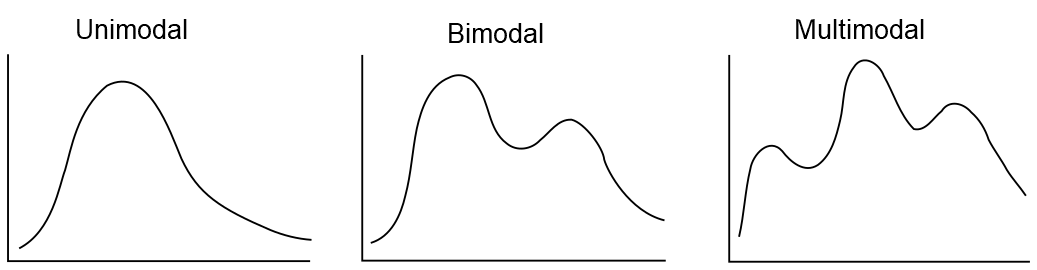
\includegraphics[width=0.8\linewidth]{_main_files/figure-latex/figUniBiMultiModal-1} \caption{Distributions with different numbers of modes.}\label{fig:figUniBiMultiModal}
\end{figure}

Sometimes there are gaps in the data, like in Figure \ref{fig:figGappy}

\begin{figure}
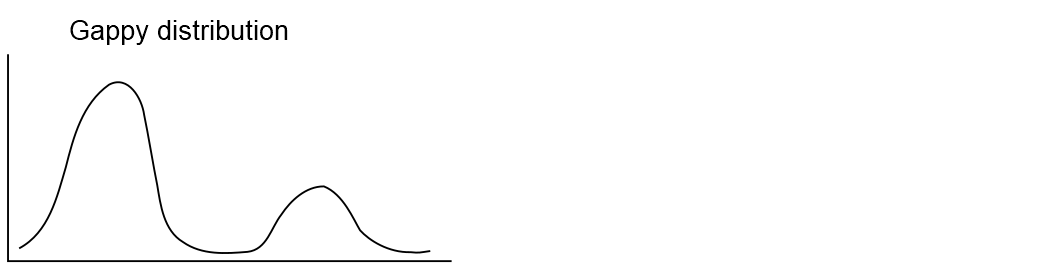
\includegraphics[width=0.8\linewidth]{_main_files/figure-latex/figGappy-1} \caption{A bimodal distribution with a gap.}\label{fig:figGappy}
\end{figure}

This can suggest the data are grouped in some way and it may be difficult
to summarise the data with single summary statistics. (Imagine Figure \ref{fig:figGappy} represents heights of people on a school trip---what could explain the distribution looking gappy like that?)

In such cases, then it may be appropriate to give, for example, more than one measure of location.

\hypertarget{visual_data-features_symmetry}{%
\subsection{\texorpdfstring{{\textbf{Symmetry}}}{Symmetry}}\label{visual_data-features_symmetry}}

The summary statistics we looked at previously were all measures of location or
spread---they tell us nothing about the symmetry of the distribution.

There is another summary statistic called \textbf{skewness} which measures the
\emph{assymmetry} of a distribution.

The sample skewness for a sample
\(x_1 , x_2 , \ldots , x_n\), of observations is defined as:

\[ g = \frac{1}{n} \sum\limits_{i=1}^n \left( \frac{x_i - {\bar{x}}}{s} \right) ^3 ,\]

where \(\bar{x}\) and \(s\) are the sample mean and standard deviation
respectively.

A perfectly symmetric distribution has a skewness of zero.

A distribution with skewness greater than zero is said to be positively
skewed, or skewed to the right (meaning the right `tail' is longer).

A distribution with skewness less than zero is said to be negatively skewed,
or skewed to the left (the left `tail' is longer).

\begin{figure}
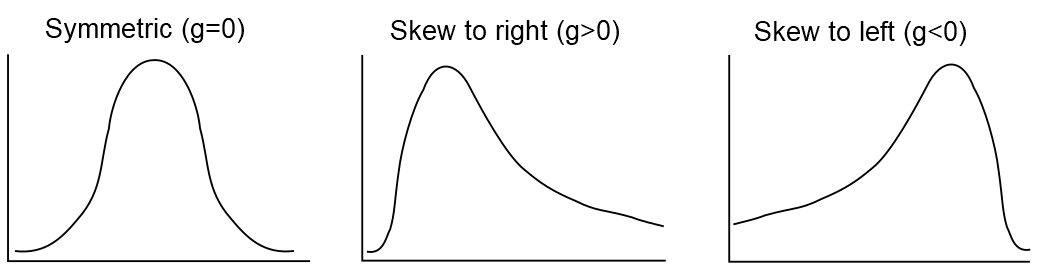
\includegraphics[width=0.8\linewidth]{_main_files/figure-latex/figSkewness-1} \caption{Symmetric and asymmetric (skewed) distributions.}\label{fig:figSkewness}
\end{figure}

\hypertarget{visual_data-features_outliers}{%
\subsection{\texorpdfstring{{\textbf{Outliers}}}{Outliers}}\label{visual_data-features_outliers}}

An outlier is an observation which is in some sense extreme. In the
context of a single sample of observations on one random variable,
outliers are observations that are well above or well below the other
values in the data. For example, the observation of 3.83 in the \protect\hyperlink{intro_example}{Cavendish dataset} considered in \protect\hyperlink{summary_robust}{Section 2.3}. All such extreme observations should be checked if
possible to ensure they are correct values. It is important to identify
any outliers in a data set as they can considerably distort numeric
summaries or analytical methods (robustness).

In cases when an observation appears to be an outlier and no reason for
the extreme measurement is found, the data could be analysed both with
the outlier included and once it has been removed. Thus the distortion
due to the outlier can be fully assessed.

\hypertarget{visual_plot}{%
\section{Basic plot types}\label{visual_plot}}

\hypertarget{visual_plot_histo}{%
\subsection{\texorpdfstring{{\textbf{Histogram and bar charts}}}{Histogram and bar charts}}\label{visual_plot_histo}}

Whenever more than about twenty observations are involved, it is often
helpful to group the observations in a \textbf{frequency table}. Frequency
tables are also helpful when constructing histograms as we shall see in
a moment. We write \(f_i\) for the frequency of observation \(x_i\)
(\(i = 1,\ldots,k)\). A frequency table shows how many observations fall
into various classes defined by categorising the observations into
groups, see the \protect\hyperlink{intro_example}{Coursework marks} example. The choice of which classes to use is somewhat arbitrary, but
since it affects the visual impression given by the data when forming a
histogram, the choice should be made with care.

The following are guidelines:

\begin{enumerate}
\def\labelenumi{\arabic{enumi}.}
\item
  For continuous data, we usually choose consecutive intervals of the
  same width. For discrete data, the individual values are used if
  this is reasonable, but if the data are sparse it may be necessary
  to classify the observations into consecutive groups of values with
  the same number of values in each group. In either case, care is
  needed when specifying the intervals so that ambiguities are
  avoided.
\item
  Interval or group sizes should be chosen so that most frequencies
  (of observations in a class) are of a moderate size compared with
  the total number of observations. For example, data on the heights
  of 100 individuals which range from 160cm to 190cm might be grouped
  easily in intervals of 2cm or possibly 5cm but not 1mm or 50cm.
\end{enumerate}

Once we have constructed a frequency table we can construct a
\textbf{histogram} easily as the data have already been grouped. When drawing
a histogram the classification intervals are represented by the scale on
the abscissa (`x-axis') of a graph (N.B. sometimes the midpoints of the
intervals are used as the scale on the abscissa) and rectangles are
drawn on this base so that the \emph{area} of the rectangle is \emph{proportional
to the frequency} of observations in the class. The unit on the ordinate
(`y-axis') is the number of observations per unit class interval. Note
that the \emph{heights} of the rectangle will be \emph{proportional to
frequencies} if and only if class intervals of \emph{equal} size are used.

Histograms are usually given in terms of \emph{frequency} (number of occurrences) but can alternatively be given in terms of \emph{density}. Density rescales the histogram so that the area in the rectangles sum to one. The shape of the histogram is thus not affected but the y-axis is rescaled. Frequency has a simple interpretation whereas density allows us to compare two samples of different size (heights of the population of Nottingham, approximately 337,000 individuals with heights of the population of Long Eaton, approximately 39,000 individuals) and to compare with probability distributions.

\leavevmode\vadjust pre{\hypertarget{example007}{}}%
\textcolor{red}{Example 3.3.1.}
{ \textbf{IQ Scores} } The I.Q. of 100 people chosen at random was
measured, resulting in the following frequency table:

\begin{longtable}[]{@{}cr@{}}
\toprule\noalign{}
\endhead
\bottomrule\noalign{}
\endlastfoot
I.Q. & \# of people (frequency) \\
IQ \(\leq\) 80 & 0 \\
80 \(<\) IQ \(\leq\) 90 & 12 \\
90 \(<\) IQ \(\leq\) 100 & 37 \\
100 \(<\) IQ \(\leq\) 110 & 30 \\
110 \(<\) IQ \(\leq\) 120 & 19 \\
120 \(<\) IQ \(\leq\) 130 & 2 \\
\end{longtable}

A histogram of these data is:

\begin{figure}
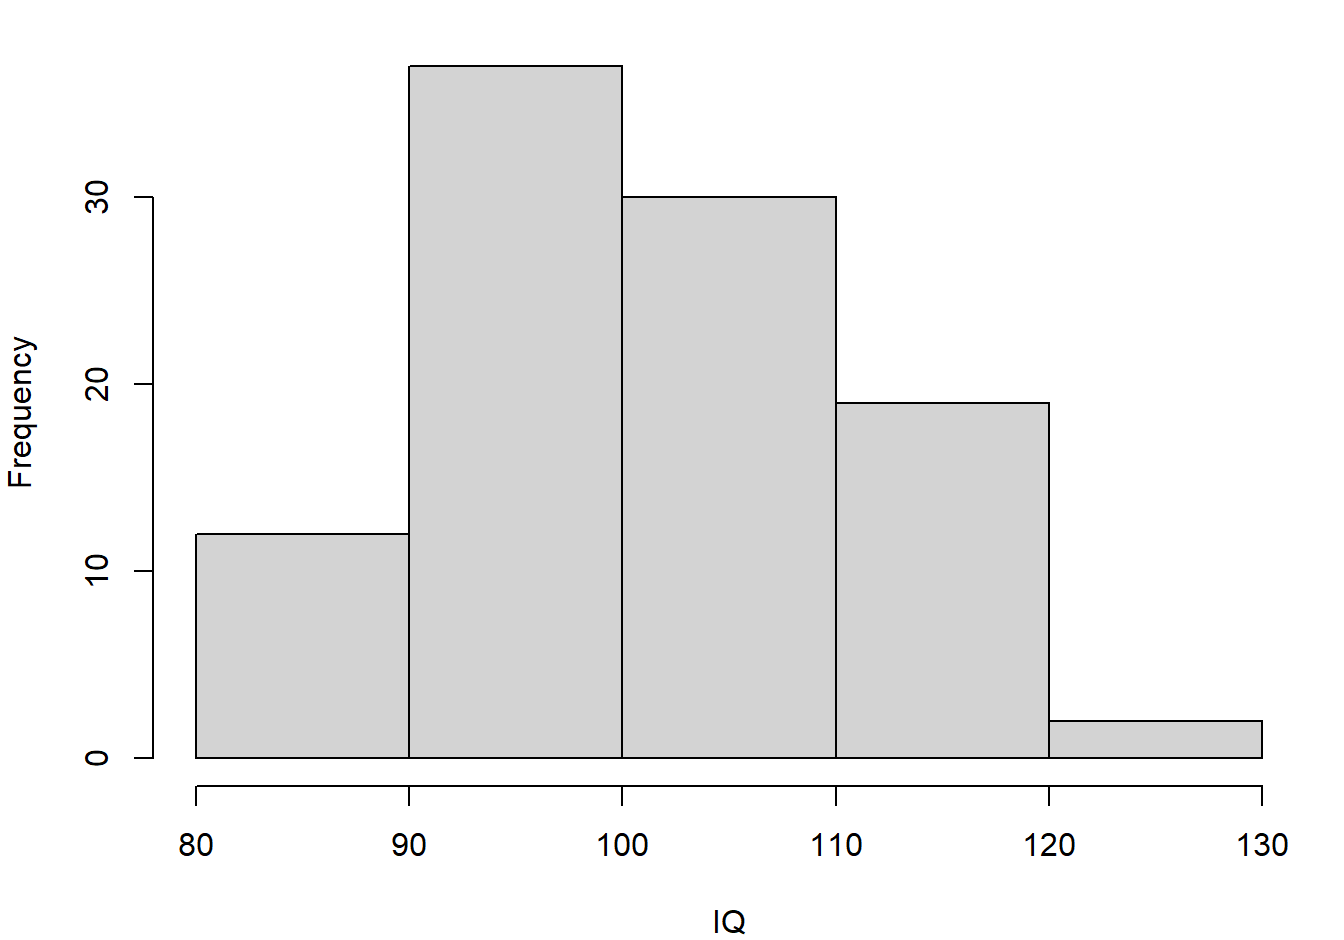
\includegraphics[width=0.8\linewidth]{_main_files/figure-latex/figIQHistogram-1} \caption{Histogram of the IQ data}\label{fig:figIQHistogram}
\end{figure}

Remember: frequency should be \emph{proportional to area}, and so for unequal
class widths one should plot the frequency density. For the IQ data, if we wanted 110-130 to be one class, compare:

\begin{figure}
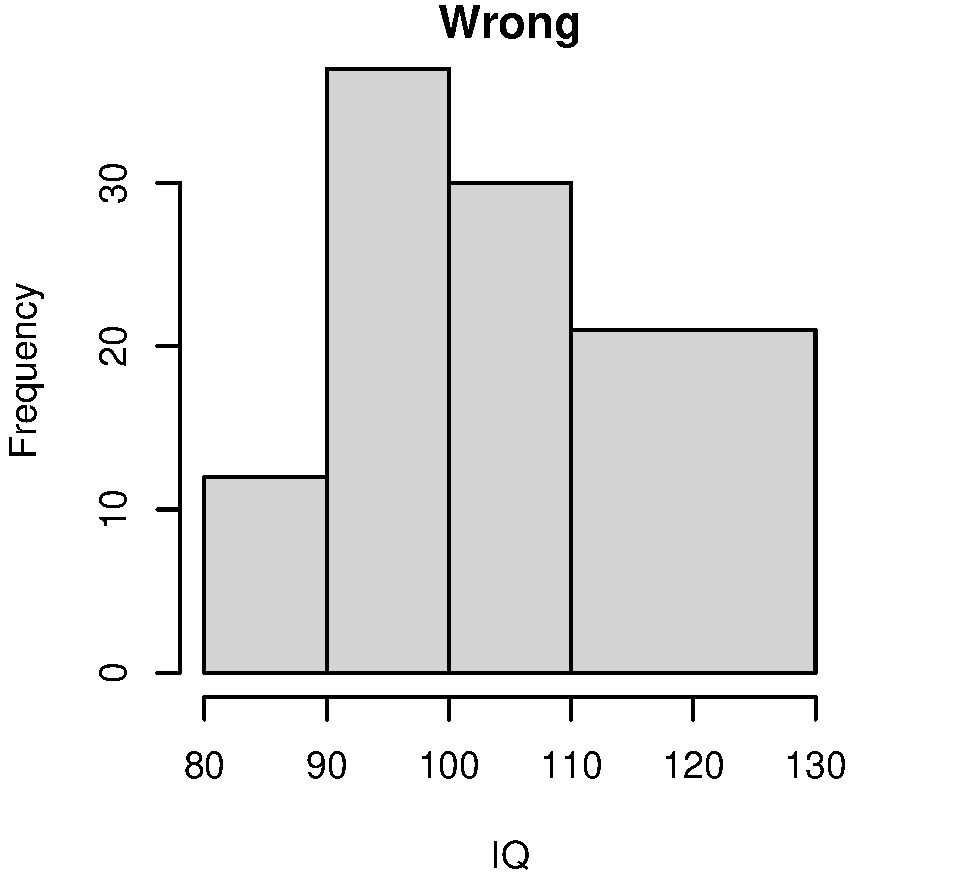
\includegraphics[width=0.45\linewidth]{_main_files/figure-latex/fig-IQ-histogram-2-1} 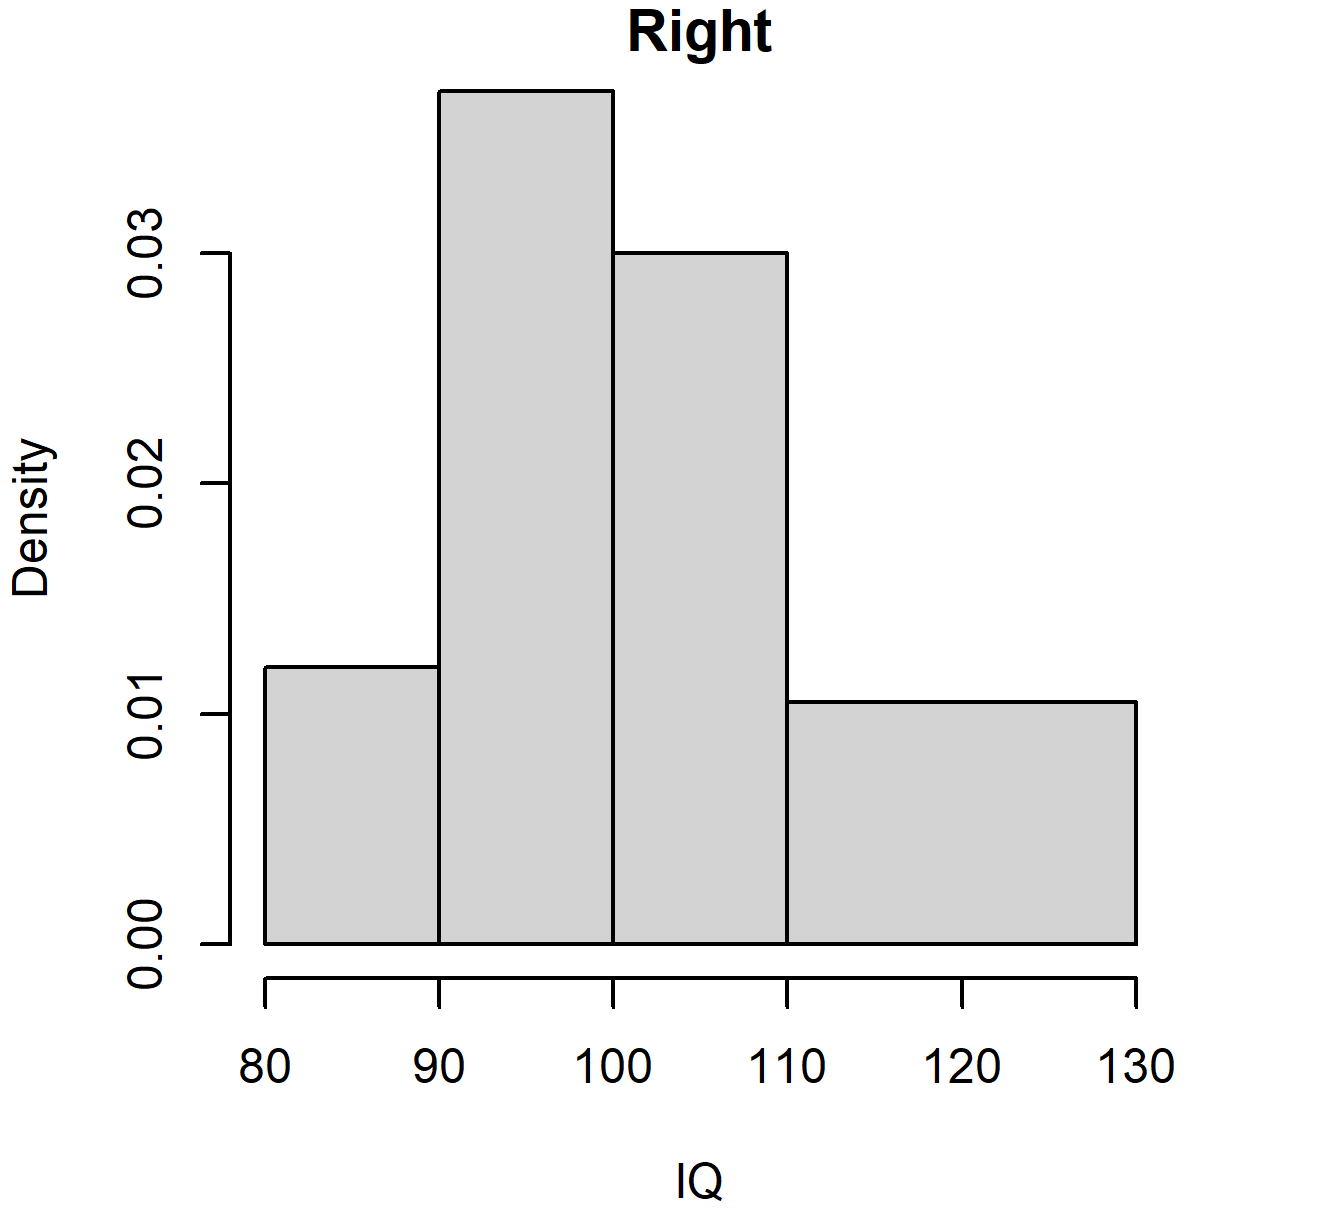
\includegraphics[width=0.45\linewidth]{_main_files/figure-latex/fig-IQ-histogram-2-2} \caption{Histogram of IQ data with unequal bar widths: wrong and right versions}\label{fig:fig-IQ-histogram-2}
\end{figure}

When the data are discrete an alternative and better form of
graphical representation is a \textbf{bar chart} with the heights of the bars
representing frequencies, see Figure \ref{fig:barg}.

\begin{figure}
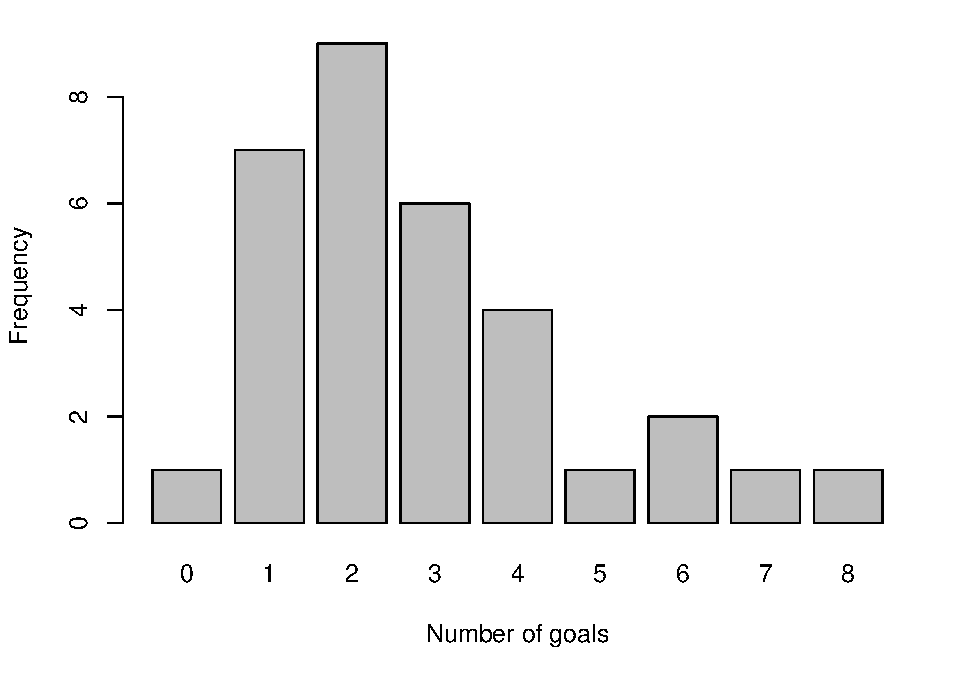
\includegraphics[width=0.8\linewidth]{_main_files/figure-latex/barg-1} \caption{Goals scored in each of 32 FA Cup third round matches}\label{fig:barg}
\end{figure}

\hypertarget{visual_plot_density}{%
\subsection{\texorpdfstring{{\textbf{Density plots}}}{Density plots}}\label{visual_plot_density}}

For continuous data, the histogram gives an approximation of the underlying distribution. The width and choice of endpoints of the intervals for the histogram affect the plot. Also for most continuous distributions we assume that a small change in value leads to a small change, up or down, in the likelihood of the value occurring. For example, the chance of an adult male being 169.9cm tall is unlikely to be very different to the chance of being 170.1cm tall. However, if we break the histogram into 5cm intervals with intervals 165cm-170cm and 170cm-175cm the height of the bars could be significantly different suggesting a big change in the likelihood of the heights.

In Figure \ref{fig:histograms-intervals} are 3 histograms for the same data, a sample of heights (\emph{cm}) of 100 UK adult males. Histograms 1 and 3 use intervals of length 5\emph{cm} but different starting points for the intervals. Histogram 2 uses intervals of length 2\emph{cm}.

\begin{figure}
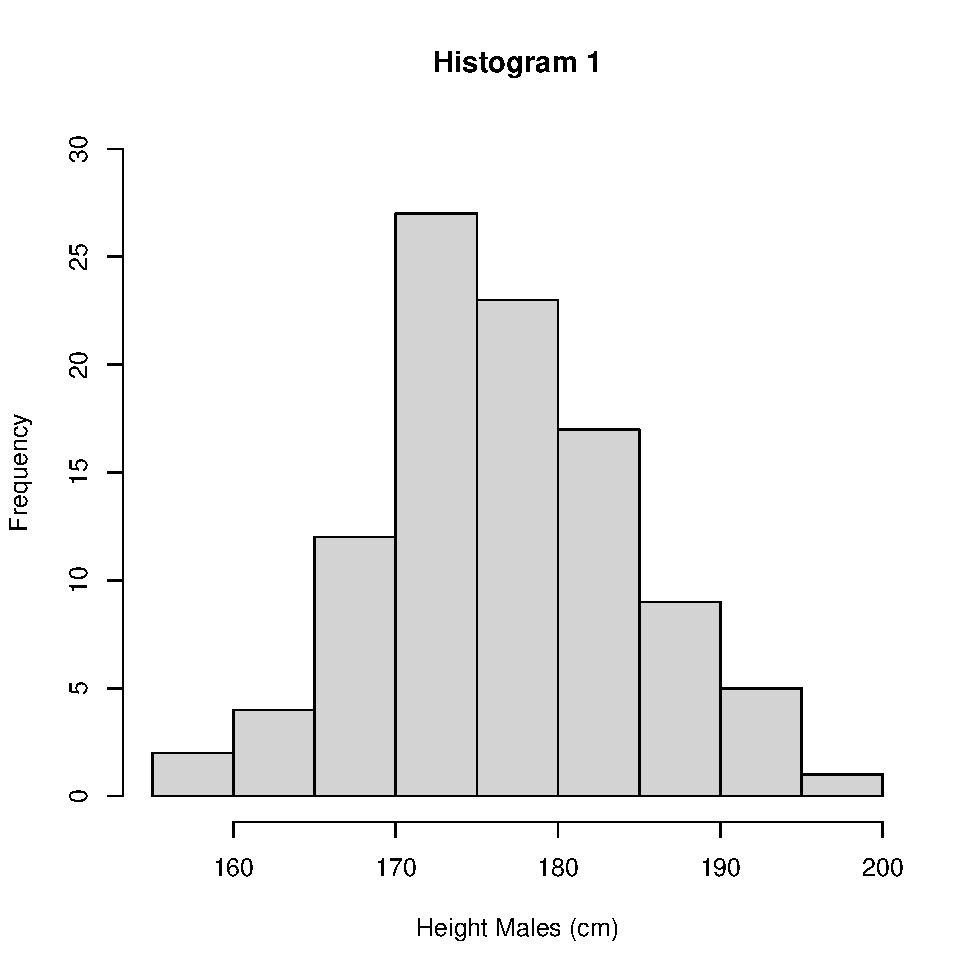
\includegraphics[width=0.33\linewidth]{_main_files/figure-latex/histograms-intervals-1} 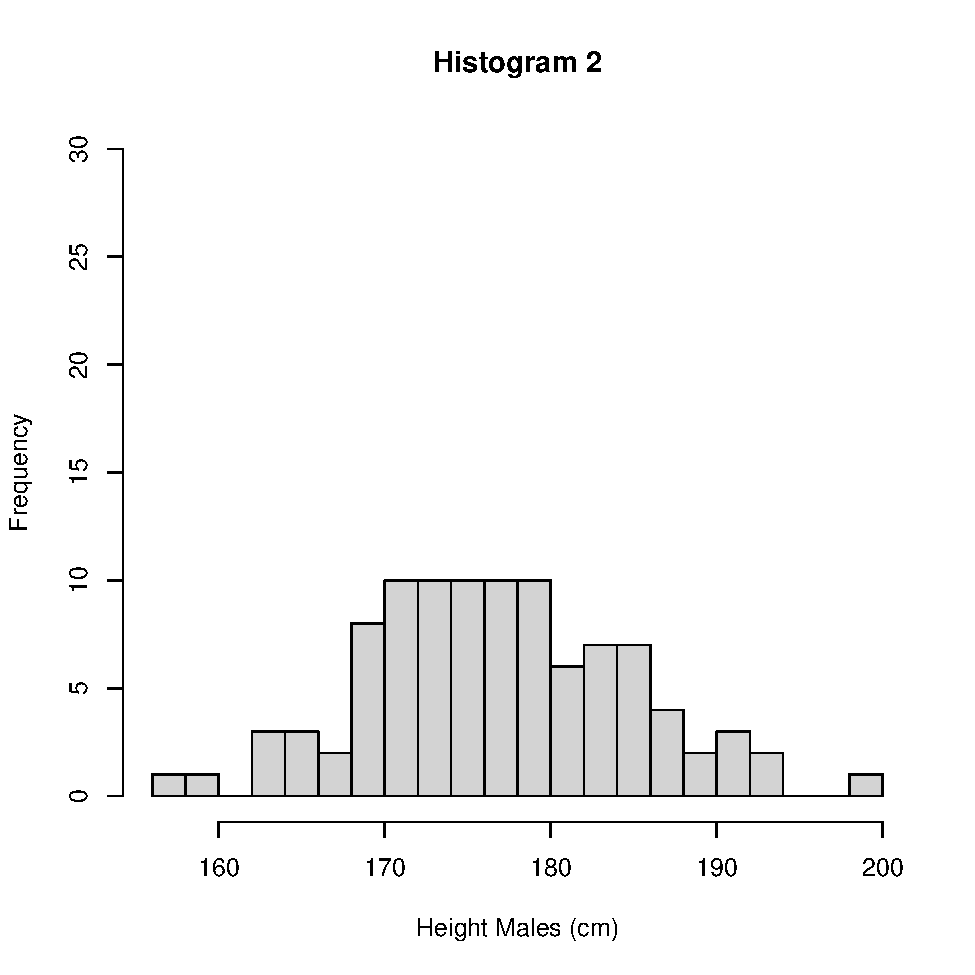
\includegraphics[width=0.33\linewidth]{_main_files/figure-latex/histograms-intervals-2} 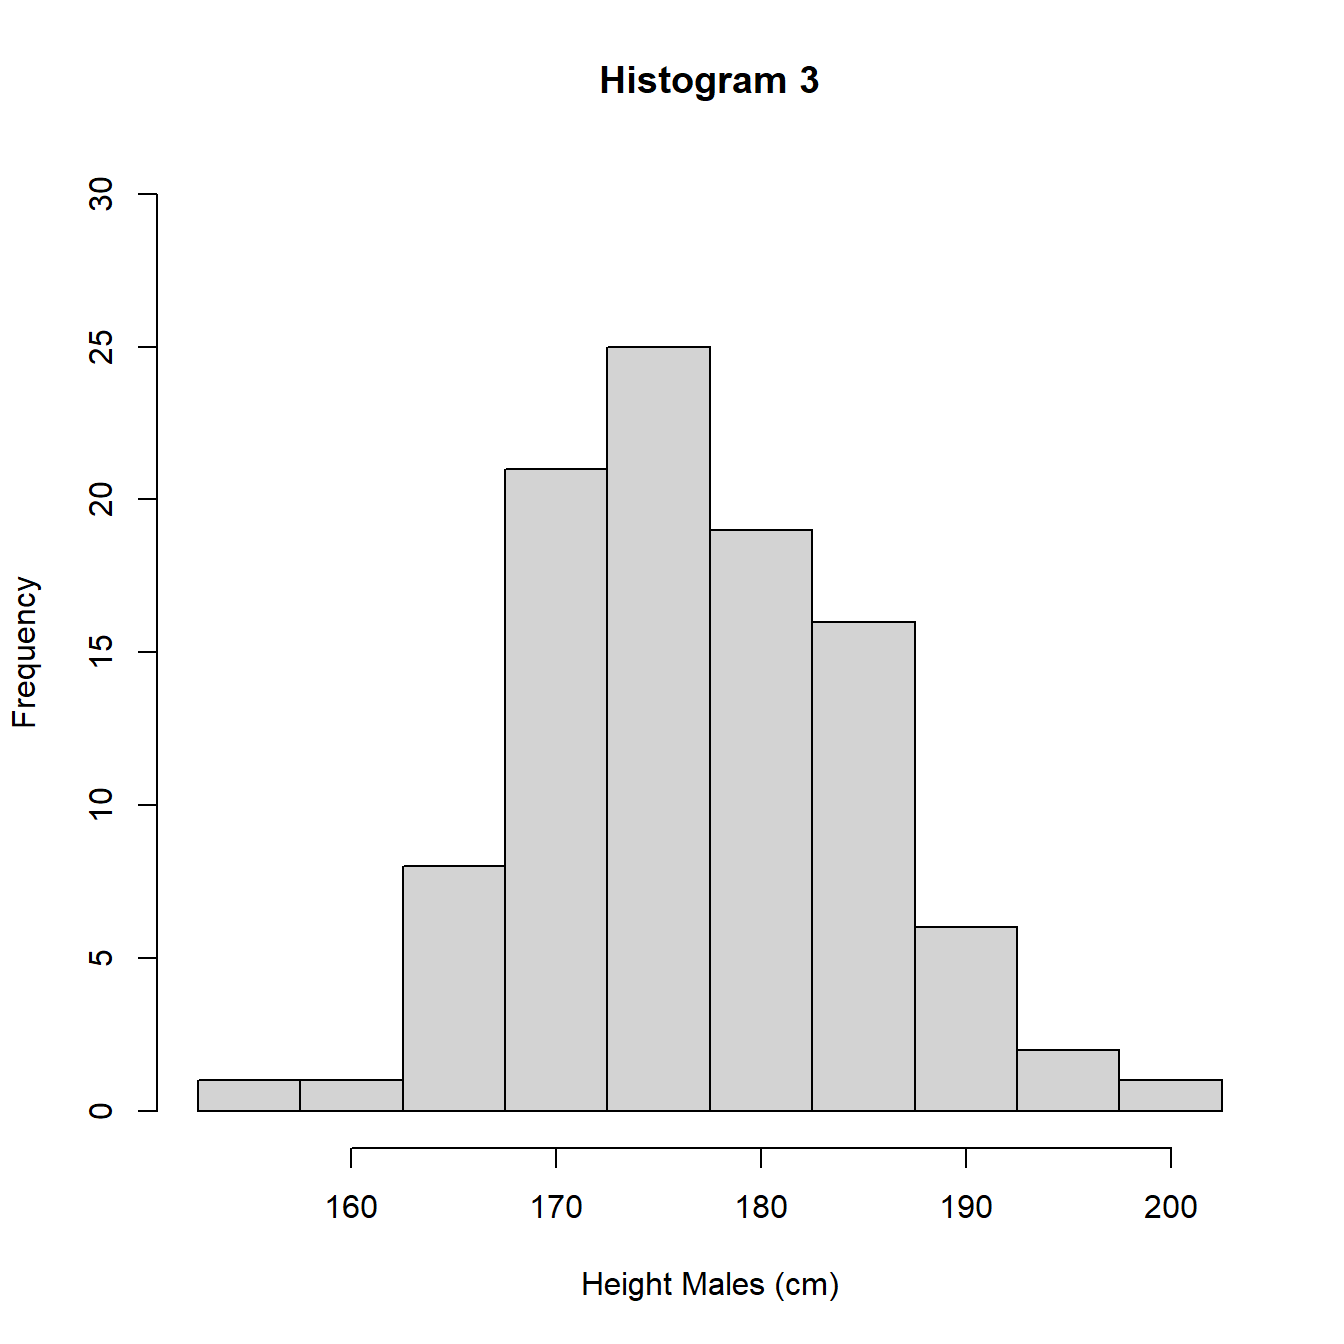
\includegraphics[width=0.33\linewidth]{_main_files/figure-latex/histograms-intervals-3} \caption{Histograms with different intervals}\label{fig:histograms-intervals}
\end{figure}

The heights (frequencies) differ between histograms 1 and 3 and histogram 2 due to the different interval widths. In Figure \ref{fig:histograms-intervals-den} we re-plot the histograms using density so the areas sum to 1 and we can perform a direct comparison.

\begin{figure}
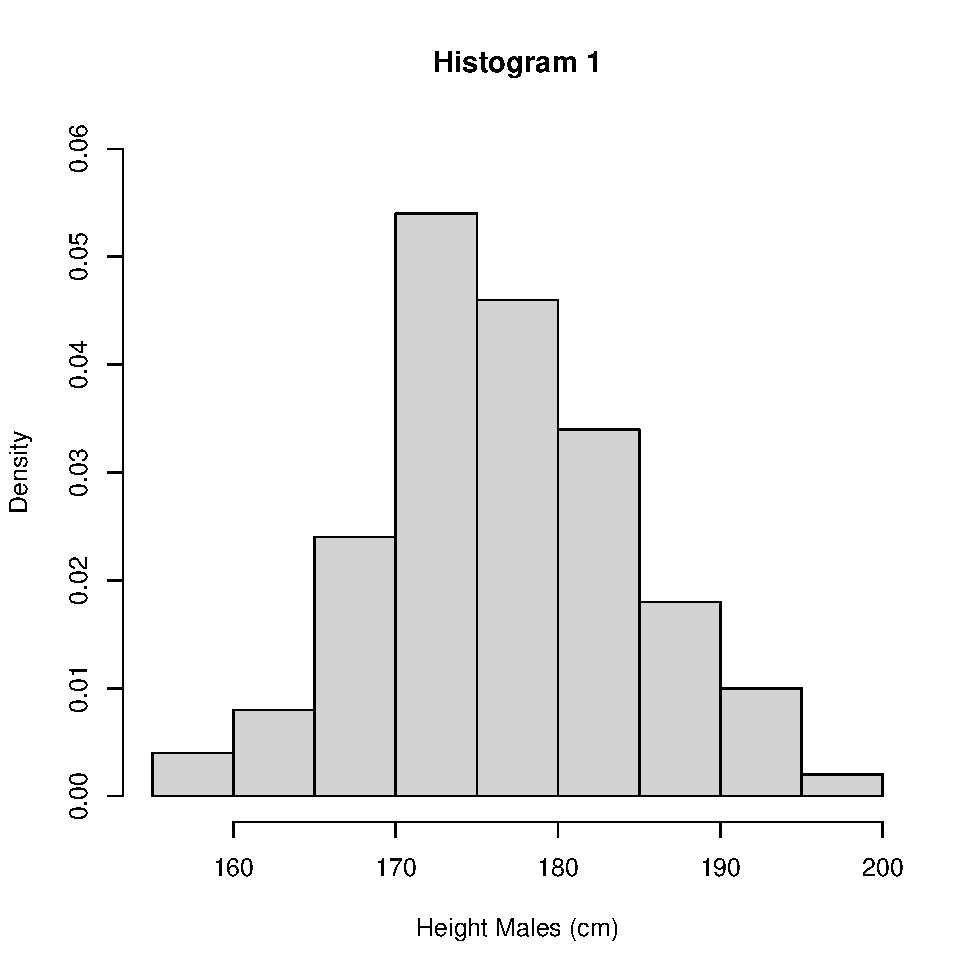
\includegraphics[width=0.33\linewidth]{_main_files/figure-latex/histograms-intervals-den-1} 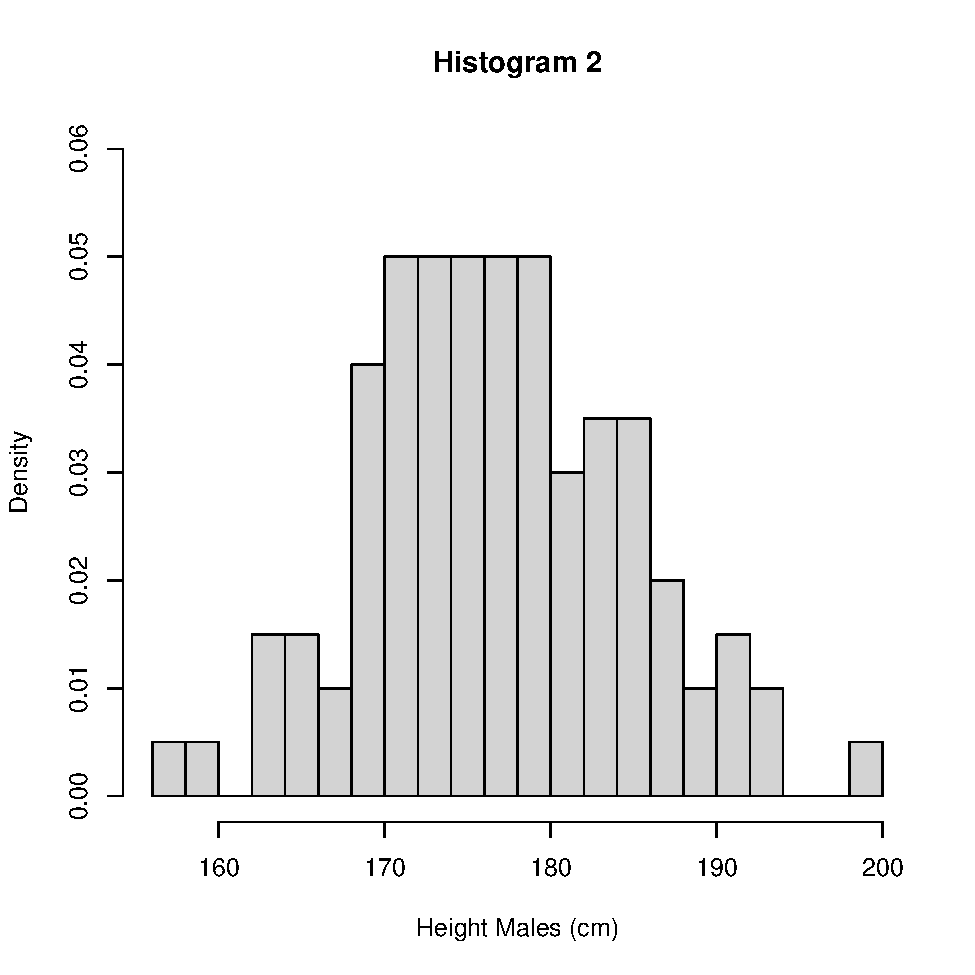
\includegraphics[width=0.33\linewidth]{_main_files/figure-latex/histograms-intervals-den-2} 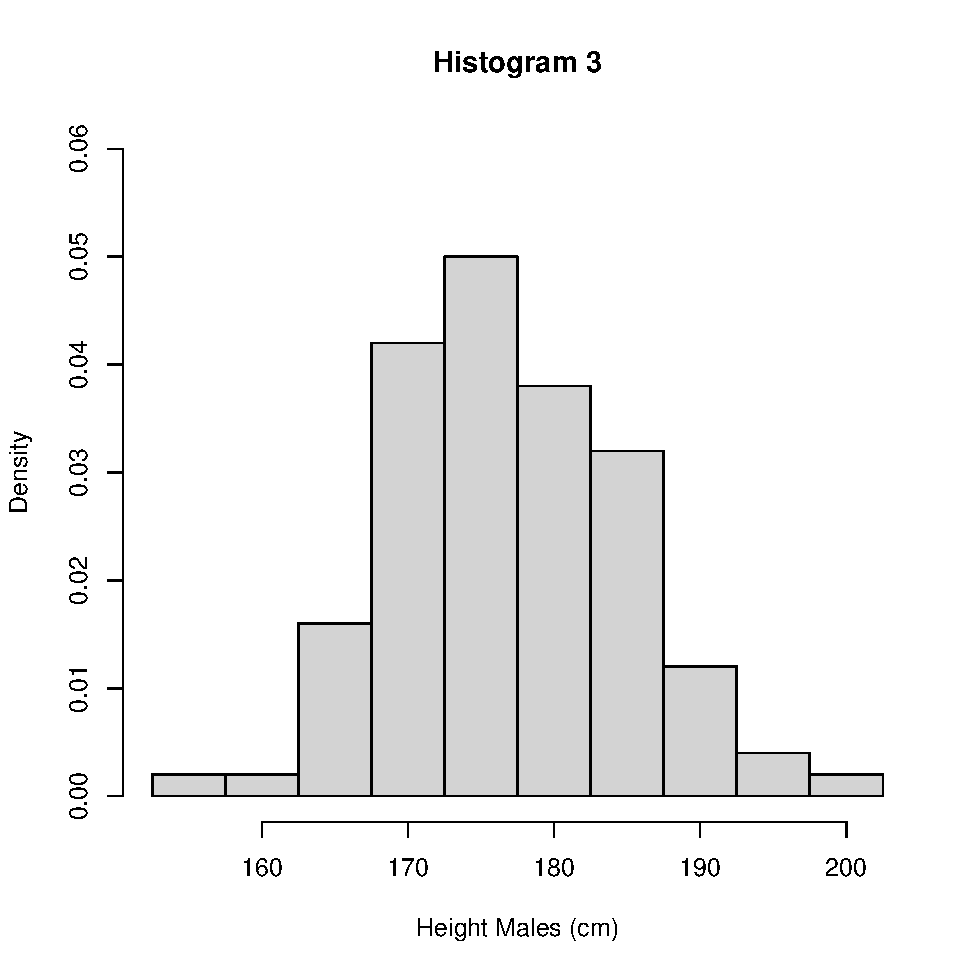
\includegraphics[width=0.33\linewidth]{_main_files/figure-latex/histograms-intervals-den-3} \caption{Histograms with different intervals}\label{fig:histograms-intervals-den}
\end{figure}

An alternative to the histogram is a density plot. A density plot uses the data to estimate the distribution of the population using an approach known as \emph{kernel smoothing}. Kernel smoothing estimates the probability density function (pdf) of the distribution of the population which is a measure of how likely a particular value is to occur. We will give a formal definition of the pdf in \protect\hyperlink{rv_des}{Section 5.2}.
This approach removes the need to specify intervals for values as for the histogram and produces a continuous approximation of the density, how likely values are. In Figure \ref{fig:density-height}, we illustrate with the UK adult male height data and also superimpose the density plot on histogram 1 to show the similarities.

\begin{figure}
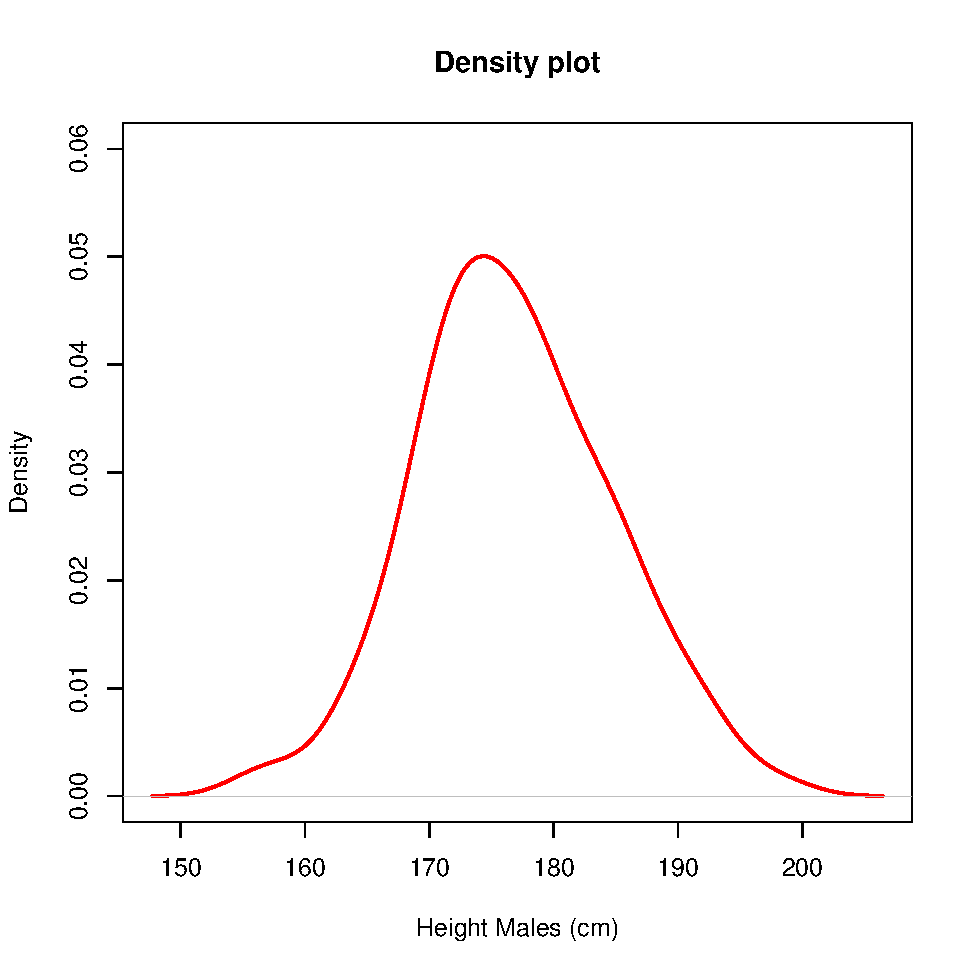
\includegraphics[width=0.4\linewidth]{_main_files/figure-latex/density-height-1} 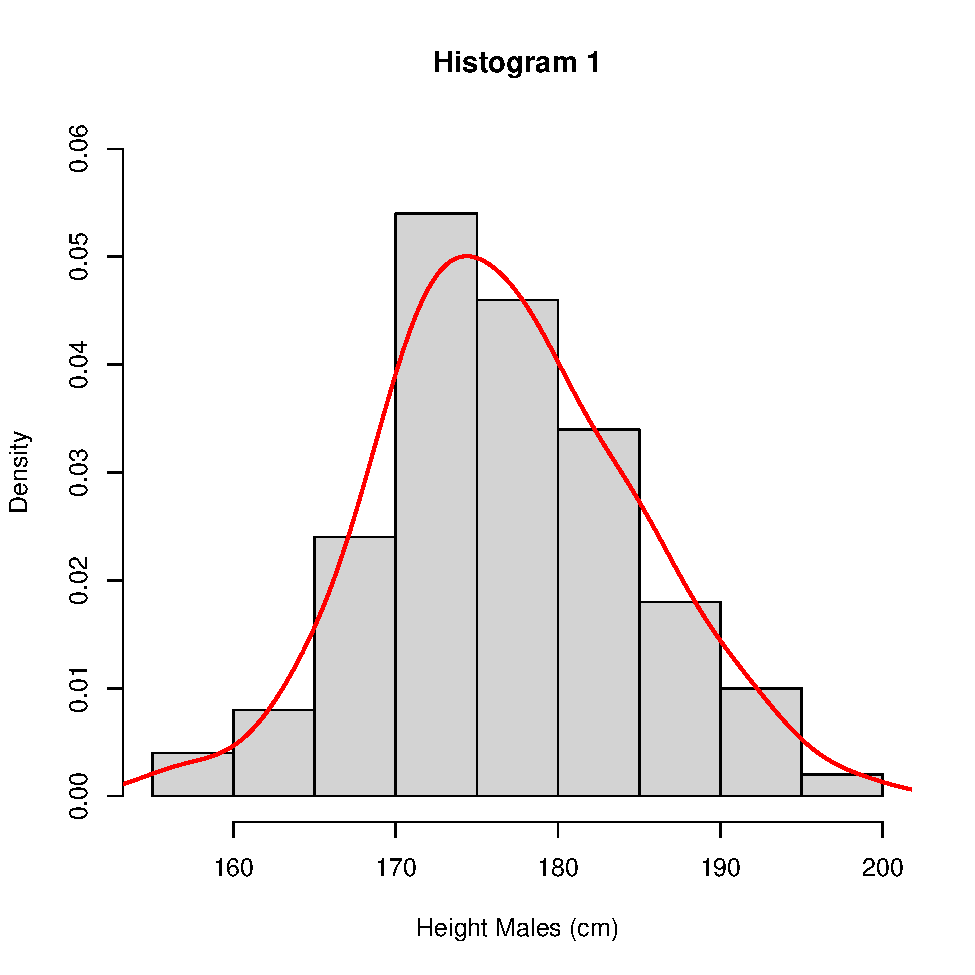
\includegraphics[width=0.4\linewidth]{_main_files/figure-latex/density-height-2} \caption{Histograms with different intervals}\label{fig:density-height}
\end{figure}

\textbf{NB.} Histograms and density plots of data may not bear much resemblance to distribution
of population when the sample size, \(n\), is \emph{small}, although as \(n\)
increases the histogram and density plot should resemble the population distribution
more closely.

In Figure \ref{fig:histograms-various-n}, we plot histograms of random samples of sizes \(n = 15, 100, 1000\) of UK adult males with the true population distribution's pdf superimposed (red).

\begin{figure}
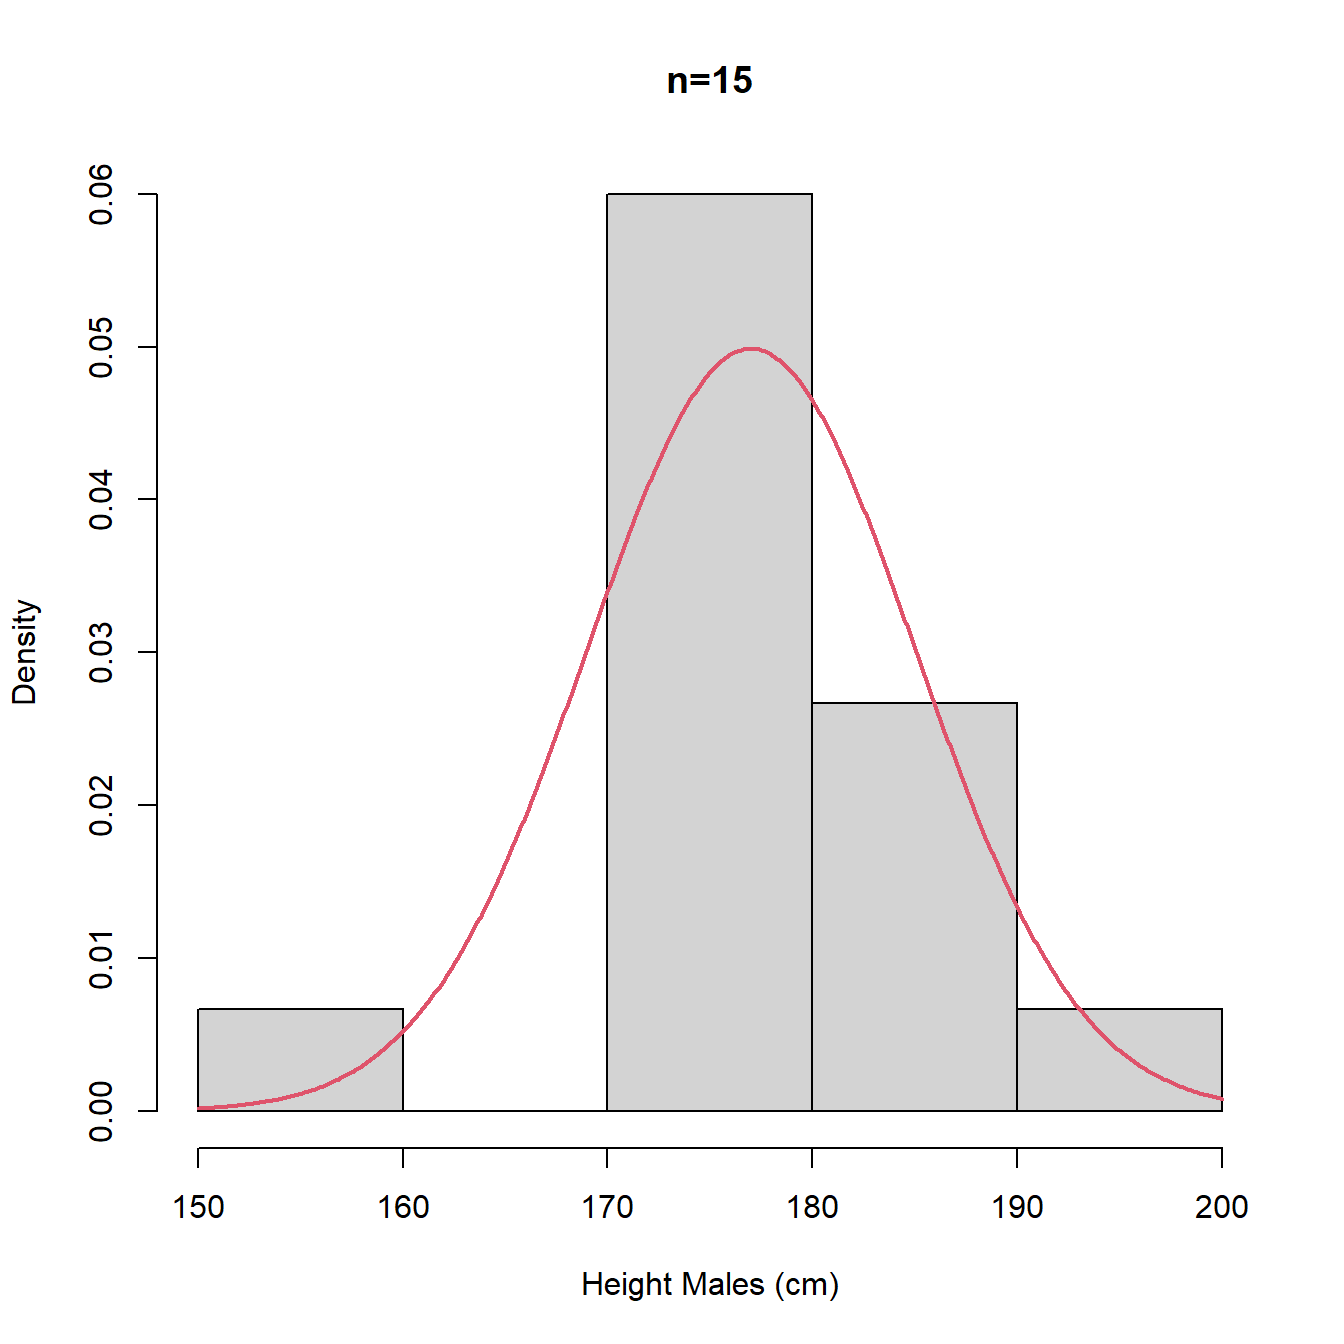
\includegraphics[width=0.33\linewidth]{_main_files/figure-latex/histograms-various-n-1} 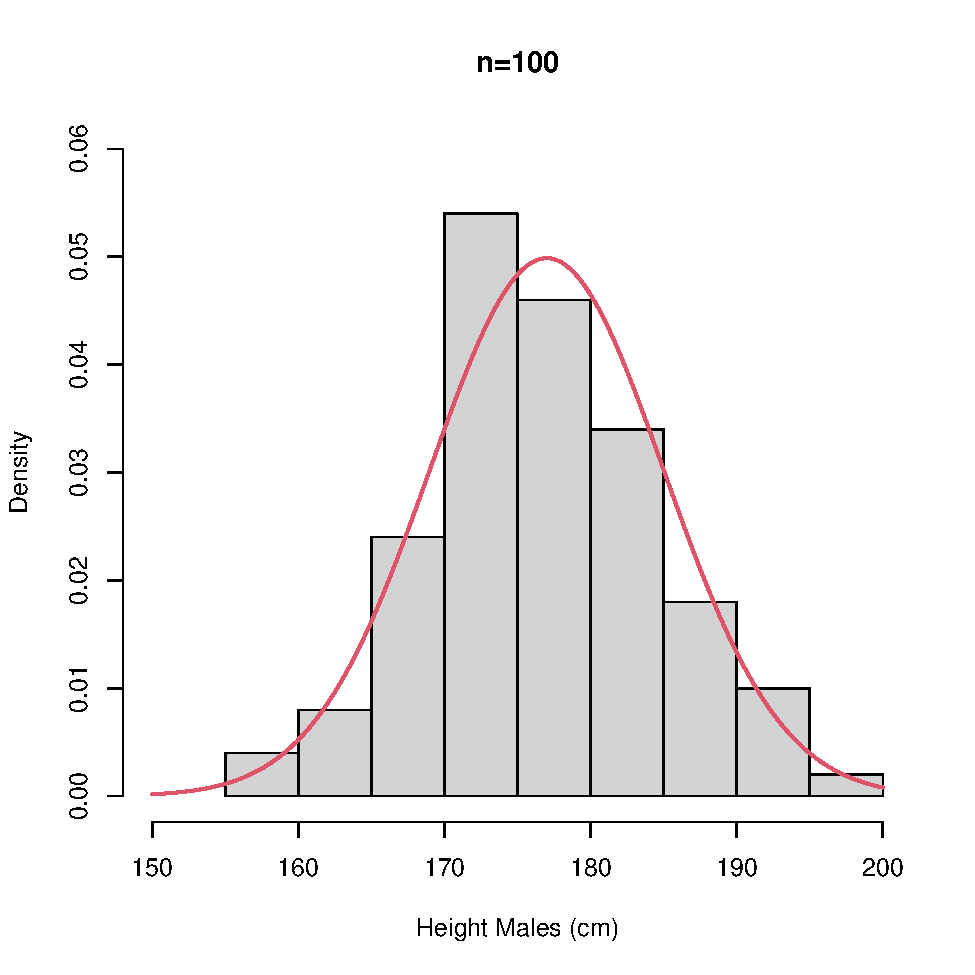
\includegraphics[width=0.33\linewidth]{_main_files/figure-latex/histograms-various-n-2} 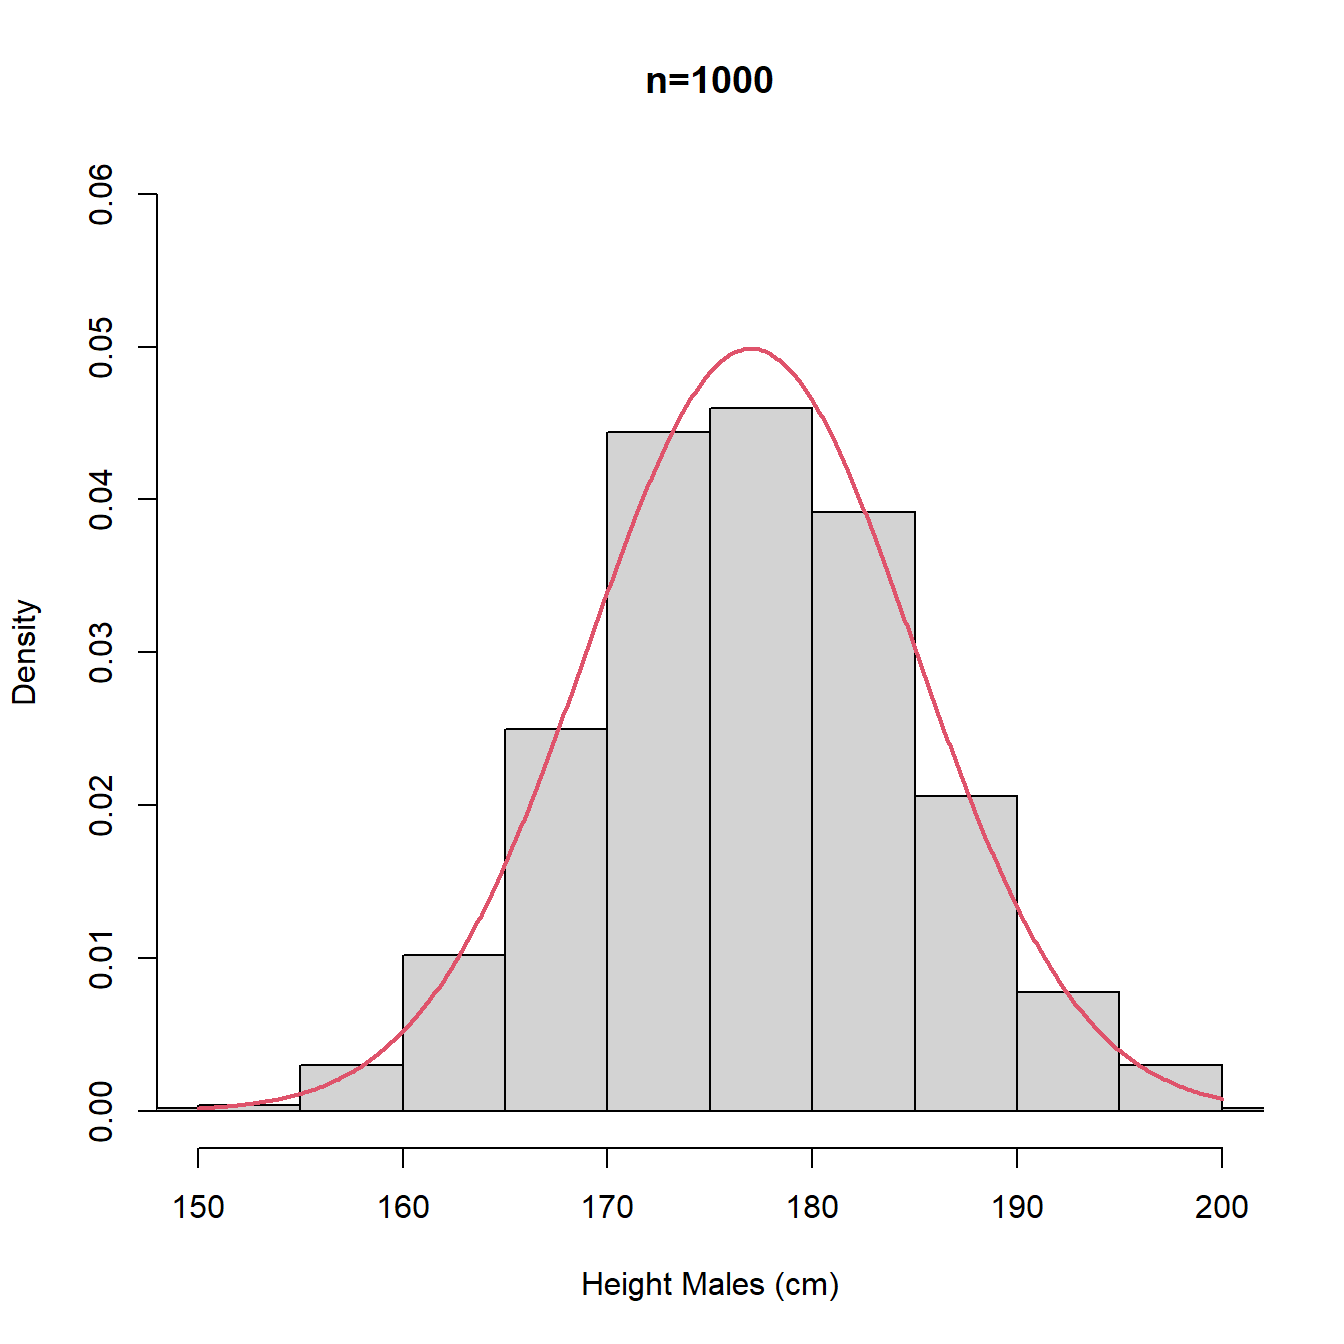
\includegraphics[width=0.33\linewidth]{_main_files/figure-latex/histograms-various-n-3} \caption{Histograms with different intervals}\label{fig:histograms-various-n}
\end{figure}

The plots in Figure \ref{fig:histograms-various-n} are repeated in Figure \ref{fig:density-various-n} using density plot instead of histogram. We note that for small \(n\) the density plot (estimate of the pdf) is rather bumpy with multiple modes and we would probably prefer the stability and unimodality of the histogram, whereas for large \(n\), the density plot (estimate of the pdf) offers a better approximation for the underlying continuous distribution (true population pdf).

\begin{figure}
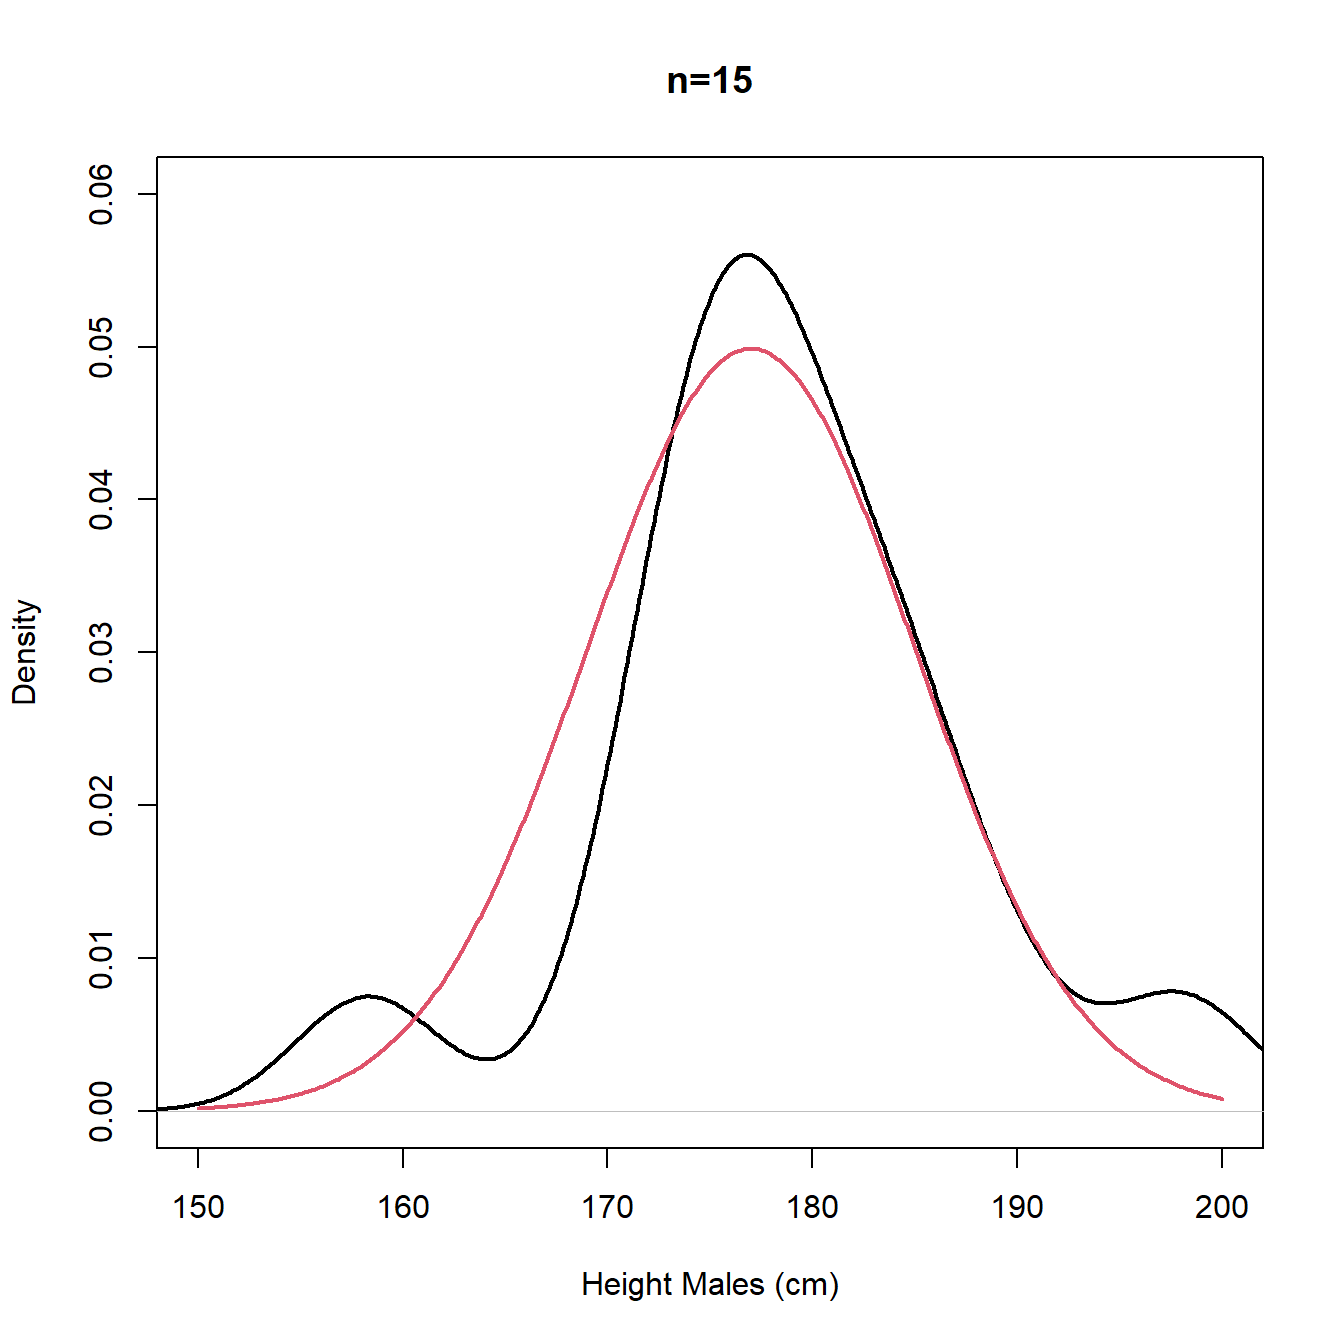
\includegraphics[width=0.33\linewidth]{_main_files/figure-latex/density-various-n-1} 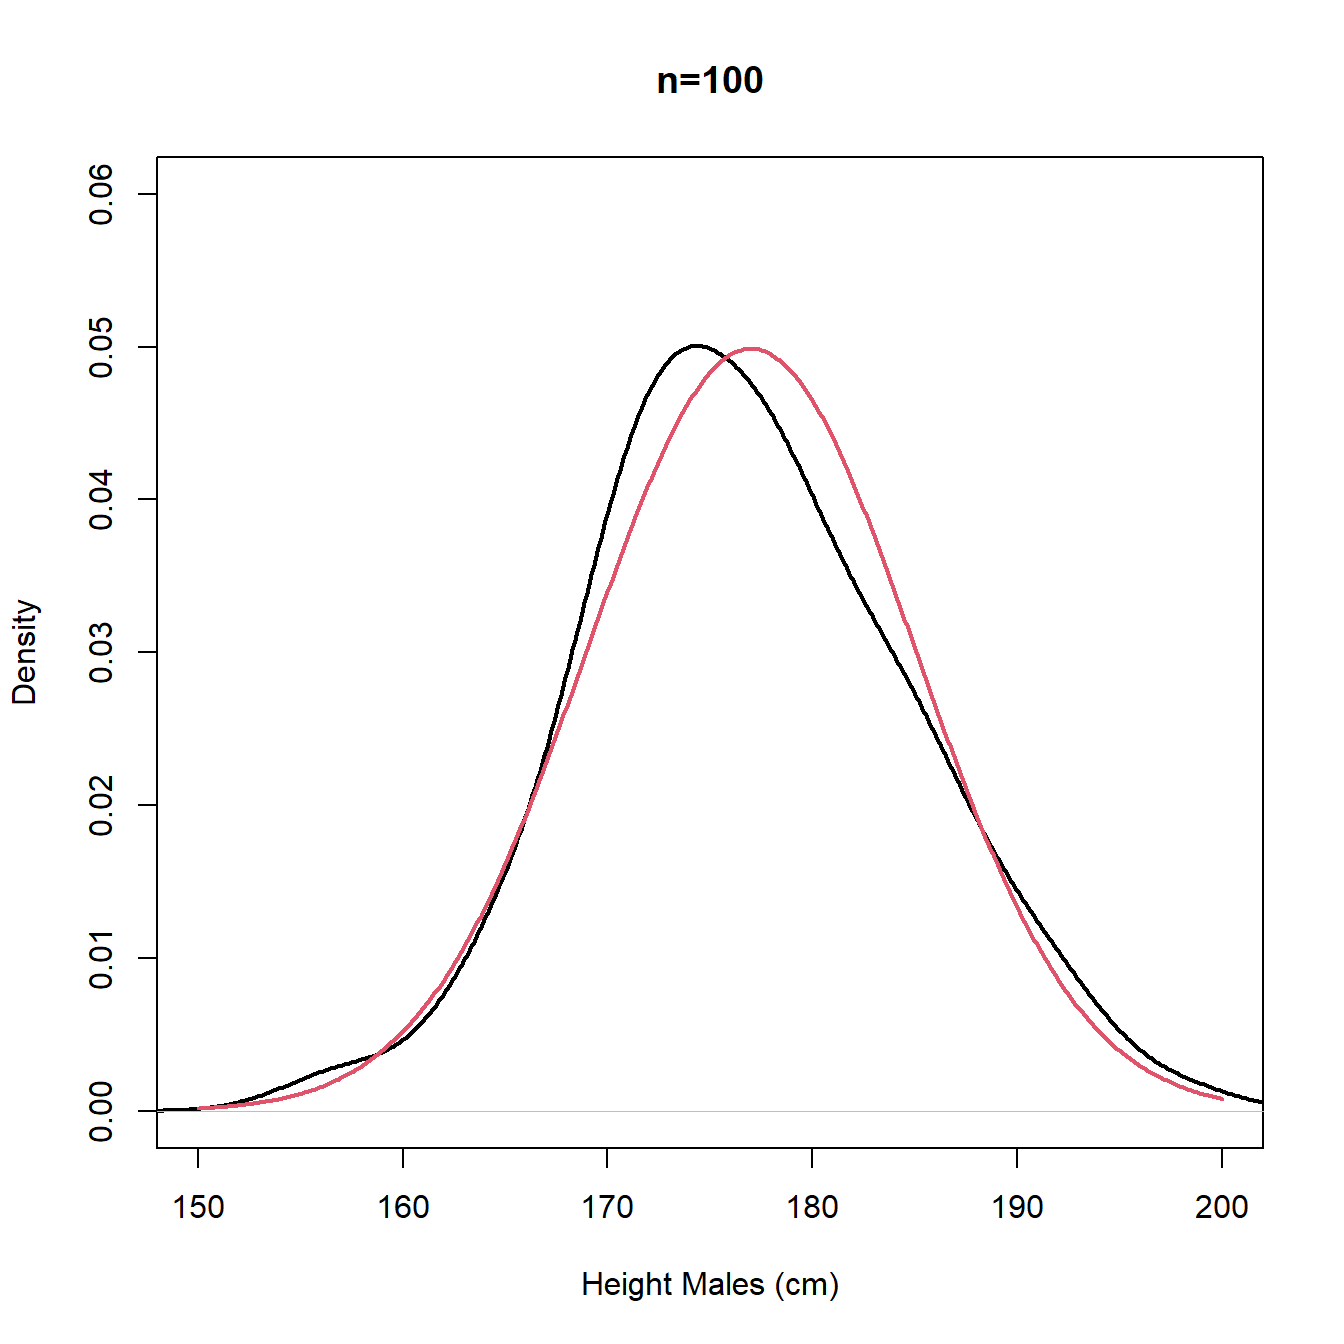
\includegraphics[width=0.33\linewidth]{_main_files/figure-latex/density-various-n-2} 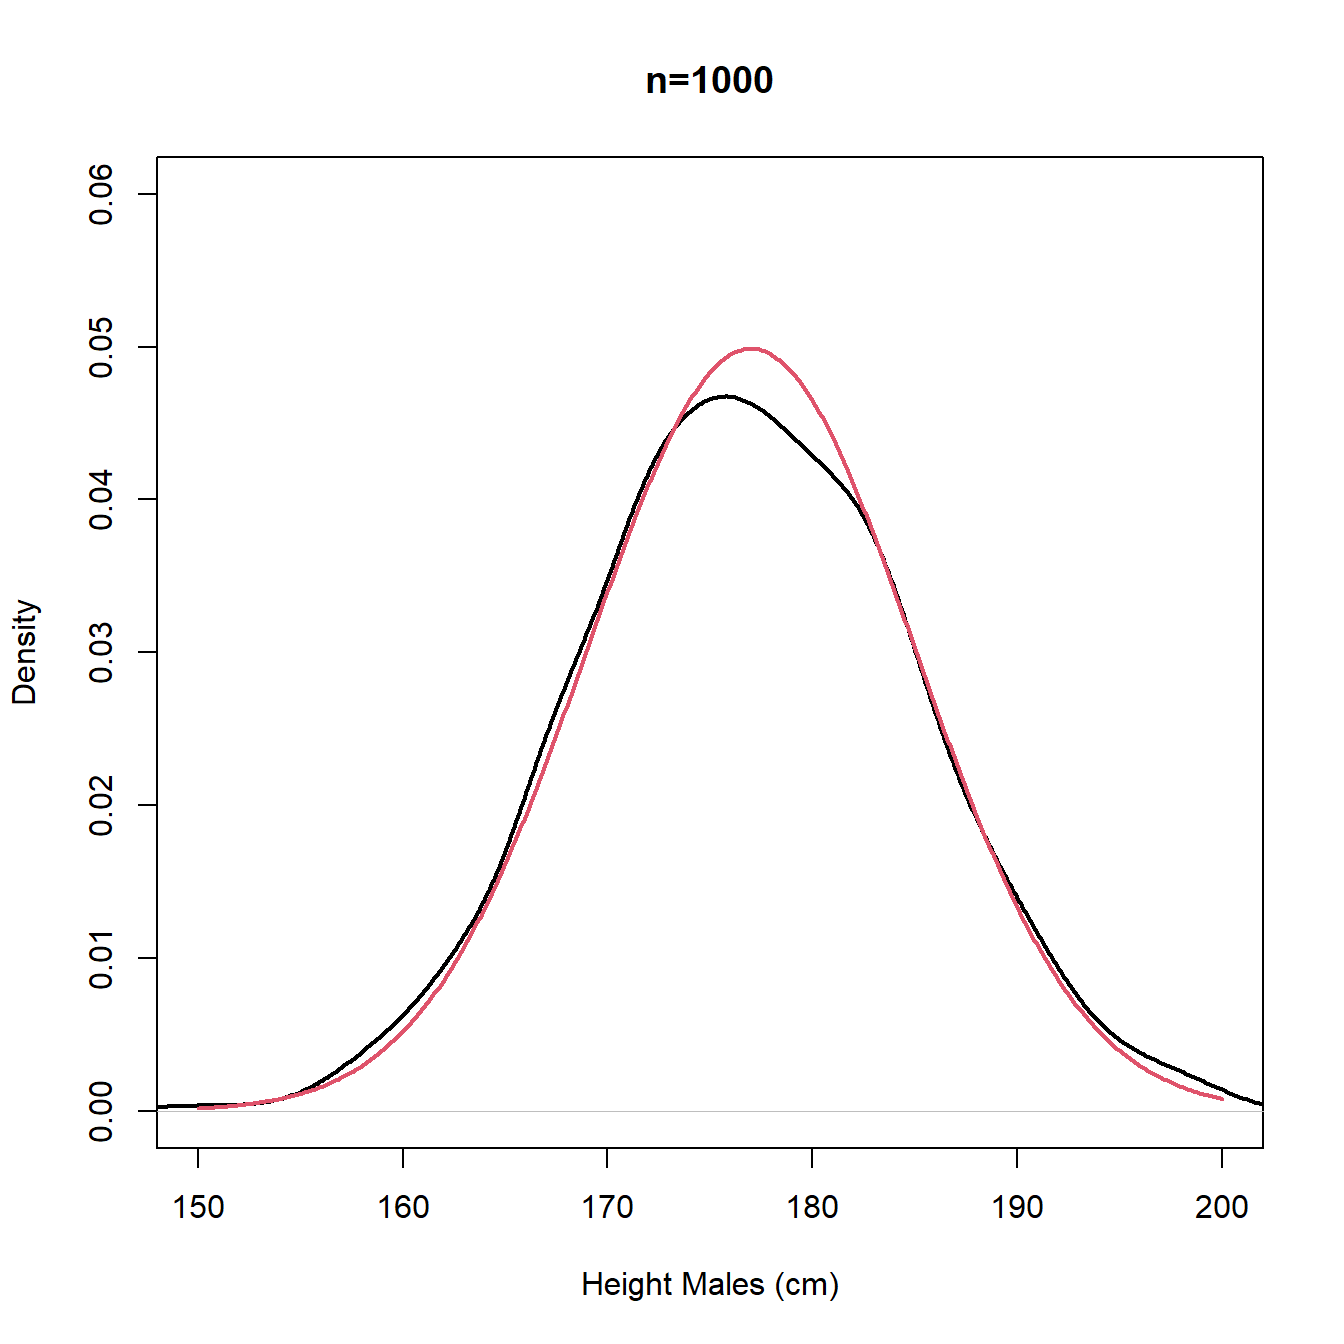
\includegraphics[width=0.33\linewidth]{_main_files/figure-latex/density-various-n-3} \caption{Density plots - sample (black) and population (red)}\label{fig:density-various-n}
\end{figure}

The following \textbf{R} Shiny app allows you to investigate data features along with histograms and density plots further for a data set comprising of marks of 3 groups of students on a maths test.

R Shiny app: \href{https://shiny-new.maths.nottingham.ac.uk/pmzpn/DataFeatures/}{Data Features}

\hypertarget{visual_plot_boxplot}{%
\subsection{\texorpdfstring{{\textbf{Boxplot}}}{Boxplot}}\label{visual_plot_boxplot}}

We have already seen that the lower quartile, median and upper quartile
split the data into four portions. Together with the lowest value in the
sample and the highest value in the sample, these statistics form the
\emph{five-number summary}:

\leavevmode\vadjust pre{\hypertarget{example008}{}}%
\textcolor{red}{Example 3.3.2.}
{ \textbf{Coursework marks} }\\
The \emph{five-number summary} for the coursework marks data given in \protect\hyperlink{intro_example}{Section 1.4} are:

\begin{longtable}[]{@{}ccccc@{}}
\toprule\noalign{}
min & \(Q_1\) & median & \(Q_3\) & max \\
\midrule\noalign{}
\endhead
\bottomrule\noalign{}
\endlastfoot
34 & 44 & 46 & 48 & 50 \\
\end{longtable}

Between each statistic fall 25\% of the observations. The simplest form
of the \textbf{boxplot} is simply a visual presentation of the five number
summary as follows:

\begin{figure}
\centering
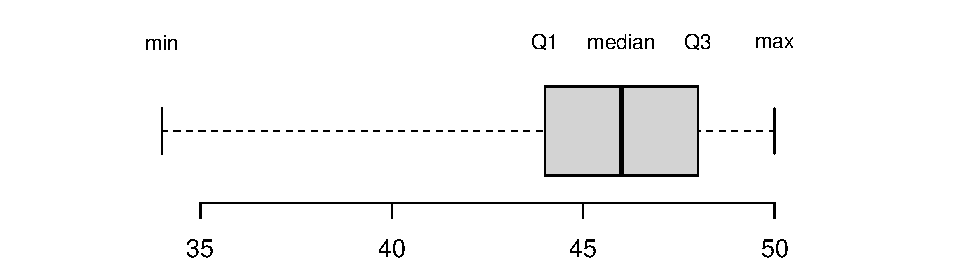
\includegraphics{_main_files/figure-latex/unnamed-chunk-18-1.pdf}
\caption{\label{fig:unnamed-chunk-18}A boxplot depicting the five-number summary}
\end{figure}

\newpage

Here the box is drawn with its left hand edge at the lower quartile
and right hand edge at the upper quartile. A line is drawn at the median
that divides the box in two. From the centre of each end of the box, a
line is drawn to the minimum and maximum of the values in the sample.
These lines are sometimes called \textbf{whiskers} and the plots are
sometimes called box-and-whisker plots. There are other variations of
the boxplot but this is the simplest version. Sometimes
extreme observations called \textbf{outliers} (see later) are picked out and denoted
with either a `*' or `o' to stop them from influencing the whiskers too
much. In fact, the \texttt{boxplot} function in \textbf{R} does this by default:

\begin{figure}
\centering
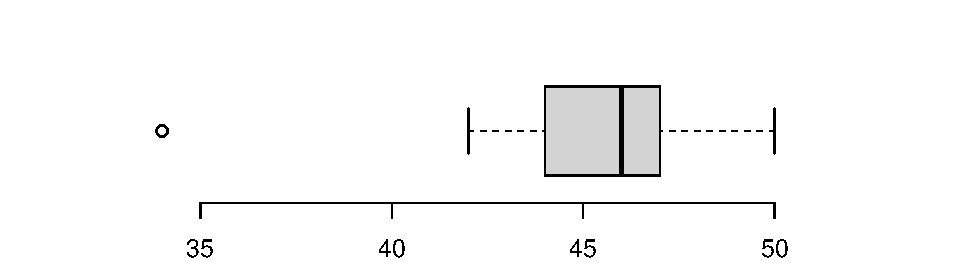
\includegraphics{_main_files/figure-latex/unnamed-chunk-20-1.pdf}
\caption{\label{fig:unnamed-chunk-20}A boxplot with an outlier picked out}
\end{figure}

\hypertarget{visual_plot_cdf}{%
\subsection{\texorpdfstring{{\textbf{Cumulative frequency diagrams, and the empirical CDF}}}{Cumulative frequency diagrams, and the empirical CDF}}\label{visual_plot_cdf}}

The \textbf{cumulative frequency} at \(x\) is defined as the number of
observations less than or equal to \(x\). The \emph{relative} cumulative
frequency, often written as \(\hat{F}(x)\), is the cumulative frequency of \(x\) divided by the total number of
observations \(n\).

\(\hat{ F}(x)\) is also called the \textbf{empirical cumulative distribution
function} (empirical cdf). The cumulative distribution function (cdf) for the population, denoted \(F(x)\), is the probability of observing an observation in the population taking a value less than or equal to \(x\). \(F(x)\) is an increasing (strictly non-decreasing) function in \(x\) with the rate of change in the cdf determined by the pdf introduced in discussions of the \protect\hyperlink{visual_plot_density}{density plot}.
We will introduce the cdf formally in \protect\hyperlink{rv:des}{Section 5.2}.

A cumulative frequency diagram involves plotting the cumulative
frequency at \(x\) versus \(x\). If the data are grouped continuous data (\protect\hyperlink{example007}{IQ scores})
then straight lines are drawn between the upper class boundaries, and if
the data are discrete,goals per FA cup match, Figure \ref{fig:barg}, or ungrouped data then a step function is used. This is illustrated in Figure \ref{fig:fig-ecdfs}.

\newpage

\leavevmode\vadjust pre{\hypertarget{example007a}{}}%
\textcolor{red}{Example 3.3.3.}
{ \textbf{IQ Scores (revisited)} }\\
The cumulative frequency and relative cumulative
frequency for the I.Q. data above are:

\begin{longtable}[]{@{}rrr@{}}
\toprule\noalign{}
\endhead
\bottomrule\noalign{}
\endlastfoot
\(x\) & Cum. freq. & \(\hat F(x)\) \\
80 & 0 & 0 \\
90 & 12 & 0.12 \\
100 & 49 & 0.49 \\
110 & 79 & 0.79 \\
120 & 98 & 0.98 \\
130 & 100 & 1.00 \\
\end{longtable}

\begin{figure}
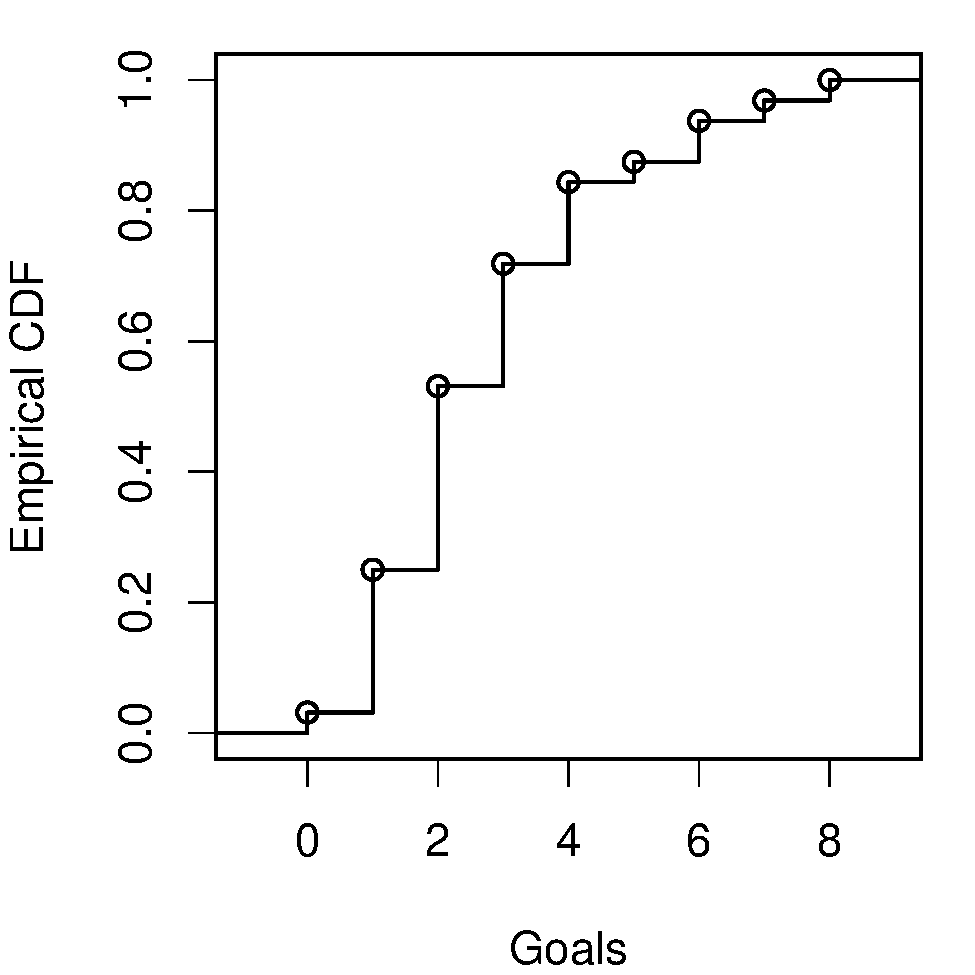
\includegraphics[width=0.45\linewidth]{_main_files/figure-latex/fig-ecdfs-1} 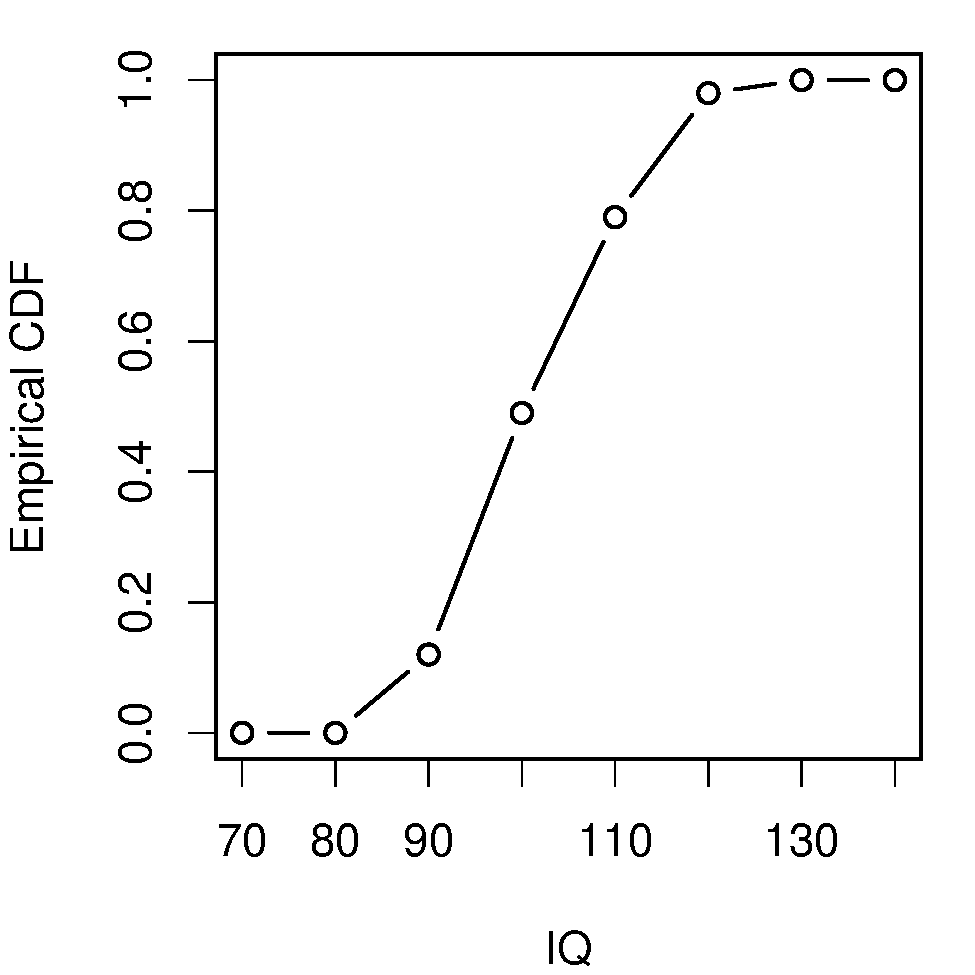
\includegraphics[width=0.45\linewidth]{_main_files/figure-latex/fig-ecdfs-2} \caption{Empirical cdf plots for the 'Goals' and 'IQ' data sets}\label{fig:fig-ecdfs}
\end{figure}

The median can be estimated from a cumulative frequency diagram by
finding the value \(x\) corresponding to cumulative frequency of \(n/2\) (or
\(\hat F(x) = 0.5\) if using the empirical CDF).

In \protect\hyperlink{video5}{Video 5} we study comparing the empriical distribution (pdf and cdf) with the random variable (population) the observations come from. This comparison is done using an \textbf{R Shiny} app which gives the histogram and estimate of the probability density function. A link to the \textbf{R Shiny} app is provided after the video to allow you to explore these features for yourself.

Watch \href{https://mediaspace.nottingham.ac.uk/media/Empirical+PDF+and+CDF+FINAL+VERSION/1_ge0o82fd}{\textcolor{blue}{Video 5: Empirical pdf and cdf}}

R Shiny app: \href{https://shiny-new.maths.nottingham.ac.uk/pmzpn/pdf_cdf_QQ/}{pdf-cdf-QQ}

\hypertarget{visual_plot_stem}{%
\subsection{\texorpdfstring{{\textbf{Stem and leaf}}}{Stem and leaf}}\label{visual_plot_stem}}

One way of representing both discrete or continuous data is to use a
\textbf{stem-and-leaf plot}. This plot is similar to a bar chart/histogram
but contains more information. It is best described by way of an
example.

\leavevmode\vadjust pre{\hypertarget{example009}{}}%
\textcolor{red}{Example 3.3.4.}
{ \textbf{Seeds data} }\\
In the routine testing of consignments of seeds,
the following procedure is used. From a consignment 100 seeds are
selected and kept under controlled conditions. The number of seeds which
have germinated after 14 days is counted. This procedure is repeated 40
times with the following results:

\begin{longtable}[]{@{}cccccccccc@{}}
\toprule\noalign{}
\endhead
\bottomrule\noalign{}
\endlastfoot
88 & 87 & 85 & 91 & 93 & 91 & 94 & 87 & 90 & 91 \\
92 & 87 & 91 & 89 & 87 & 90 & 88 & 85 & 90 & 92 \\
89 & 86 & 91 & 92 & 91 & 91 & 93 & 93 & 87 & 90 \\
91 & 91 & 89 & 90 & 90 & 91 & 91 & 93 & 92 & 85 \\
\end{longtable}

The range of data is \(94 - 85 = 9\) and we divide this range into
intervals of fixed length as we would for a histogram.

For a stem-and-leaf plot we usually make the class interval either 0.5,
1 or 2 times a power of ten and aim for between 4 and 10 intervals. Of
course, this is sometimes not possible for very small data sets. For
these data an interval of two seems appropriate as this will give us 5
or 6 intervals. Next we draw a vertical line. On the left of this
vertical line we mark the interval boundaries in increasing order but
note only the first few digits that are in common to the observation in
the interval. This is called the \textbf{stem}. We then go through the
observations one by one, noting down the next significant digit on the
right-hand side of the appropriate stem. This forms the \textbf{leaves}. Here
we obtain:

\begin{longtable}[]{@{}lllllllllllllllllll@{}}
\toprule\noalign{}
\endhead
\bottomrule\noalign{}
\endlastfoot
8 & \textbar{} & 5 & 5 & 5 & & & & & & & & & & & & & & \\
8 & \textbar{} & 7 & 7 & 7 & 7 & 6 & 7 & & & & & & & & & & & \\
8 & \textbar{} & 8 & 9 & 8 & 9 & 9 & & & & & & & & & & & & \\
9 & \textbar{} & 1 & 1 & 0 & 1 & 1 & 0 & 0 & 1 & 1 & 1 & 0 & 1 & 1 & 0 & 0 & 1 & 1 \\
9 & \textbar{} & 3 & 2 & 2 & 2 & 3 & 3 & 3 & 2 & & & & & & & & & \\
9 & \textbar{} & 4 & & & & & & & & & & & & & & & & \\
\end{longtable}

The first stem (line) contains any values of 84 and 85, the second stem
of 86 and 87, and so on. Note that by allowing the first stem to
represent 84 \& 85 we have ensured that there are stems for 88 \& 89 and
90 \& 91 and no stem for 89 \& 90 --- a stem which would be very difficult
to enter on a plot! A final version of the plot is found by ordering the
digits within each stem. For these data the final stem-and-leaf plot is

\newpage

\begin{longtable}[]{@{}lllllllllllllllllll@{}}
\toprule\noalign{}
\endhead
\bottomrule\noalign{}
\endlastfoot
8 & \textbar{} & 5 & 5 & 5 & & & & & & & & & & & & & & \\
8 & \textbar{} & 6 & 7 & 7 & 7 & 7 & 7 & & & & & & & & & & & \\
8 & \textbar{} & 8 & 8 & 9 & 9 & 9 & & & & & & & & & & & & \\
9 & \textbar{} & 0 & 0 & 0 & 0 & 0 & 0 & 1 & 1 & 1 & 1 & 1 & 1 & 1 & 1 & 1 & 1 & 1 \\
9 & \textbar{} & 2 & 2 & 2 & 2 & 3 & 3 & 3 & 3 & & & & & & & & & \\
9 & \textbar{} & 4 & & & & & & & & & & & & & & & & \\
\end{longtable}

\hypertarget{visual_plot_pie}{%
\subsection{\texorpdfstring{{\textbf{Pie charts}}}{Pie charts}}\label{visual_plot_pie}}

When we wish to display proportions of observations in a sample that take each of a discrete
number of values, a \textbf{pie chart} is sometimes used:

\begin{figure}

{\centering 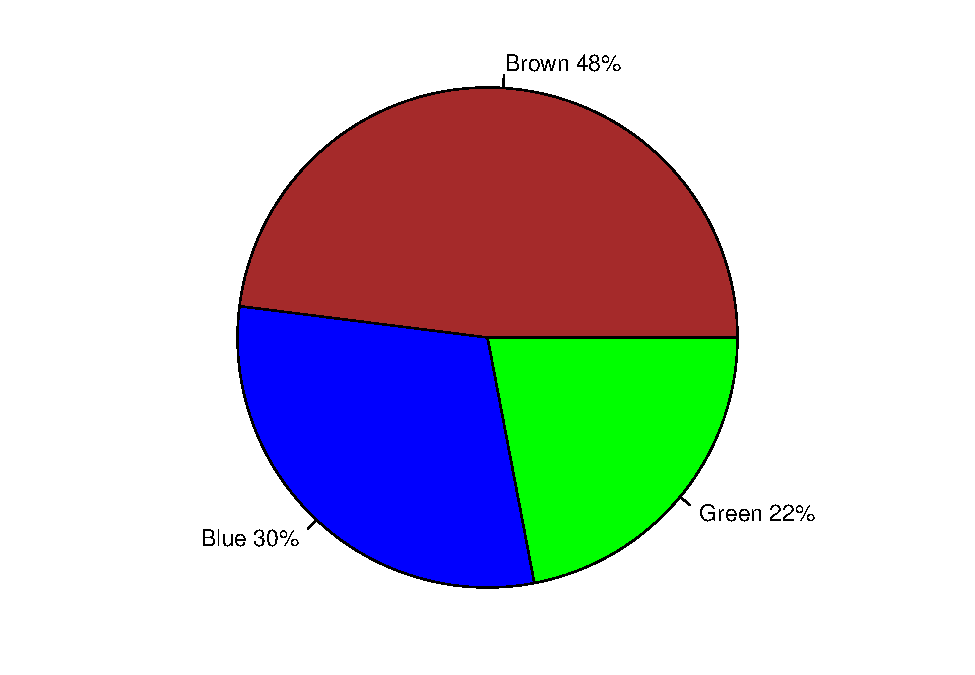
\includegraphics[width=0.9\linewidth]{_main_files/figure-latex/fig-piechart-1} 

}

\caption{Pie chart of eye colour of people in Britain}\label{fig:fig-piechart}
\end{figure}

However, there are many drawbacks with pie charts, especially when the
number of categories is large, or when some categories have small frequencies,
and the comparison of groups with similar proportions is difficult.
If you're thinking about using a pie chart then I suggest: stop, and ask yourself whether
a bar chart would be clearer!

Figure \ref{fig:opec-example-pie} is a pie chart showing the proportion of oil production by different
OPEC countries in 2016.

\begin{figure}

{\centering 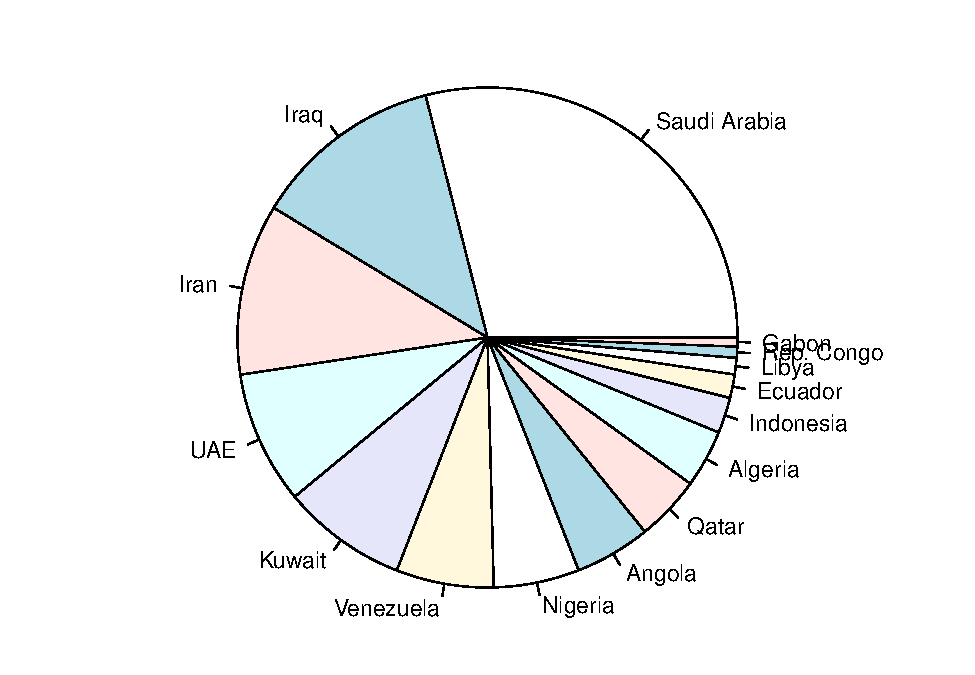
\includegraphics[width=0.9\linewidth]{_main_files/figure-latex/opec-example-pie-1} 

}

\caption{Pie chart of oil production by OPEC members}\label{fig:opec-example-pie}
\end{figure}

And Figure \ref{fig:opec-example-bar} is a bar chart showing the same data. Which do you find the clearer?

\begin{figure}

{\centering 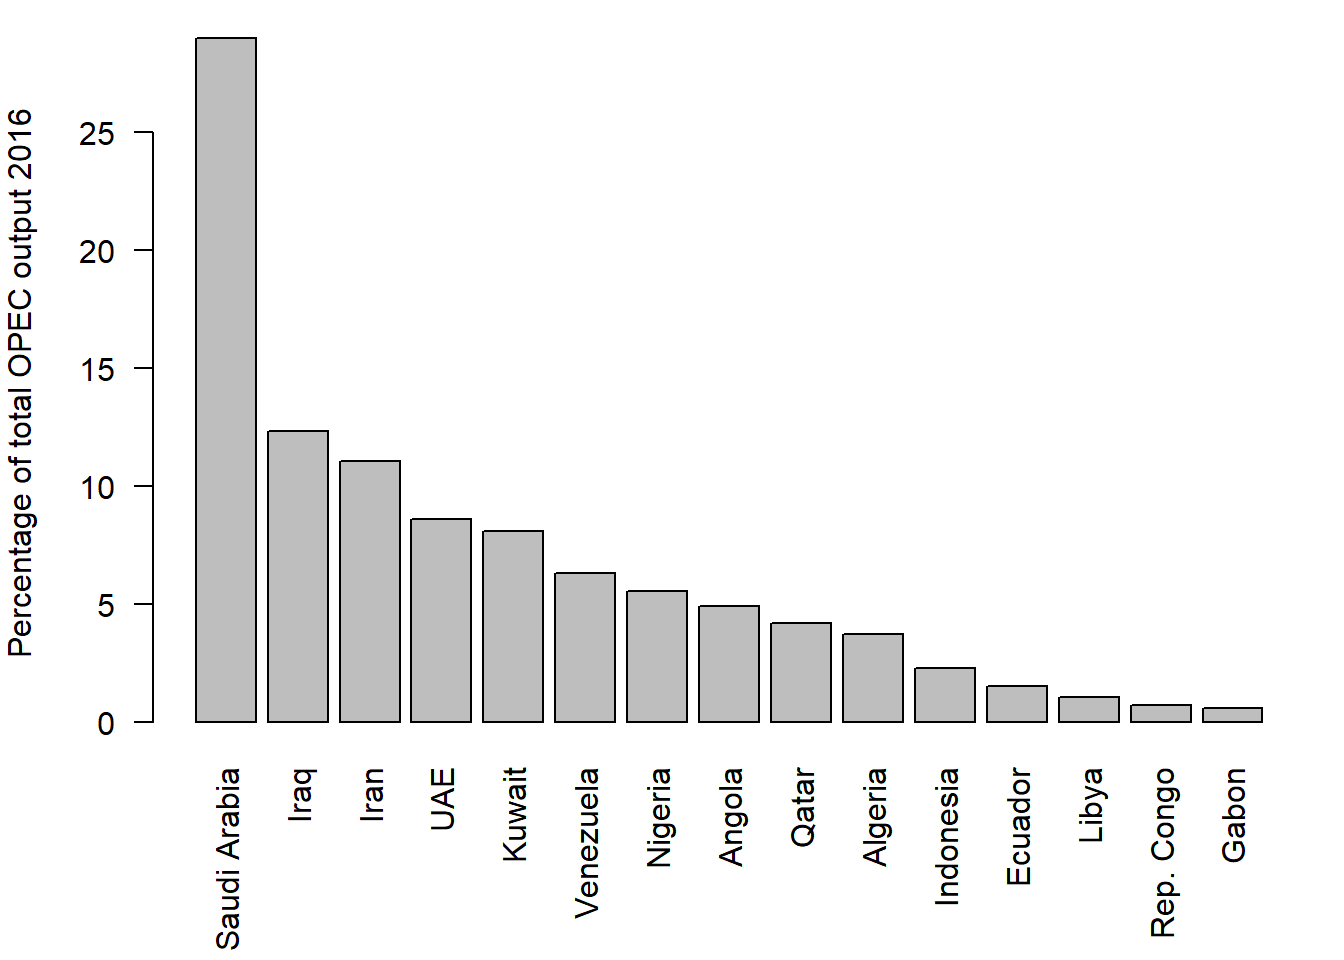
\includegraphics[width=0.8\linewidth]{_main_files/figure-latex/opec-example-bar-1} 

}

\caption{Bar chart of oil production by OPEC members}\label{fig:opec-example-bar}
\end{figure}

\hypertarget{visual_plot_dot}{%
\subsection{\texorpdfstring{{\textbf{Dotplots}}}{Dotplots}}\label{visual_plot_dot}}

A \textbf{dotplot} displays each data value as a dot, and is used for both continuous and discrete data. It is usually used only
when the sample size is small, otherwise the plot quickly gets overcrowded.
Here is a dotplot for the \(n=29\) Cavendish data values.

\begin{figure}

{\centering 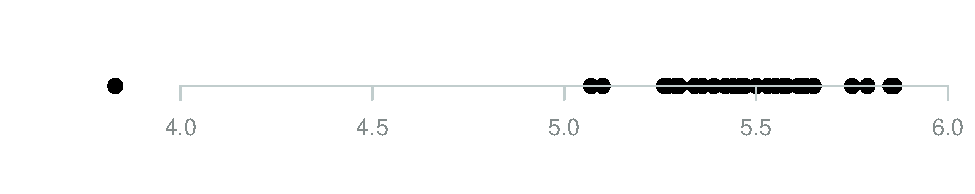
\includegraphics[width=0.95\linewidth]{_main_files/figure-latex/fig-dotplot1-1} 

}

\caption{Simple dot plot of the Cavendish data}\label{fig:fig-dotplot1}
\end{figure}

The `overplotting' makes it
difficult to see how many data values there are in the middle of the data set. Sometimes to make things a bit clear some `jitter' (randomness) is added in the y direction and/or the points are made slightly transparent, both of which help a lot in this case:

\begin{figure}

{\centering 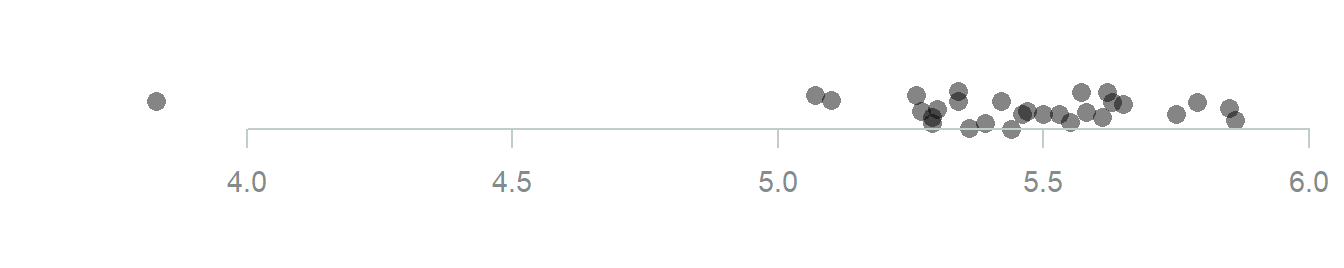
\includegraphics[width=0.95\linewidth]{_main_files/figure-latex/fig-dotplot1jittered-1} 

}

\caption{Dot plot of the Cavendish data with some jitter and transparency}\label{fig:fig-dotplot1jittered}
\end{figure}

For discrete data the dots are stacked above the
horizontal axis. The result is something
similar to a bar chart, but showing individual points.
Here is a dotplot for the
seed data:

\begin{figure}

{\centering 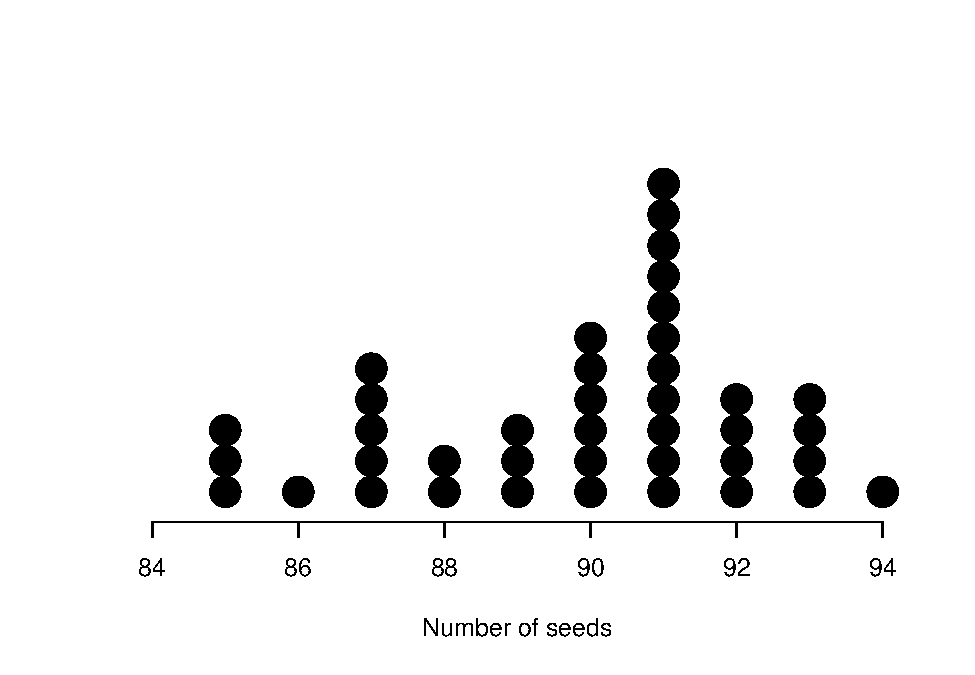
\includegraphics[width=0.65\linewidth]{_main_files/figure-latex/fig-dotplot2-1} 

}

\caption{Dot plot of some discrete seed count data}\label{fig:fig-dotplot2}
\end{figure}

\hypertarget{visual_plot_scatter}{%
\subsection{\texorpdfstring{{\textbf{Scatterplots}}}{Scatterplots}}\label{visual_plot_scatter}}

In addition to displaying the data on each random variable as above,
when we have data that consists of observations on two or more random
variables, it is useful to try and assess any relationships between
random variables by using a \textbf{scatterplot}. A scatterplot is simply a
graph with one random variable as abscissa and another random variable
as ordinate. A point is plot on the graph for each element of data at
the observed values of the two random variables,see Figure
\ref{fig:fig-scatterplot1}.

\begin{figure}

{\centering 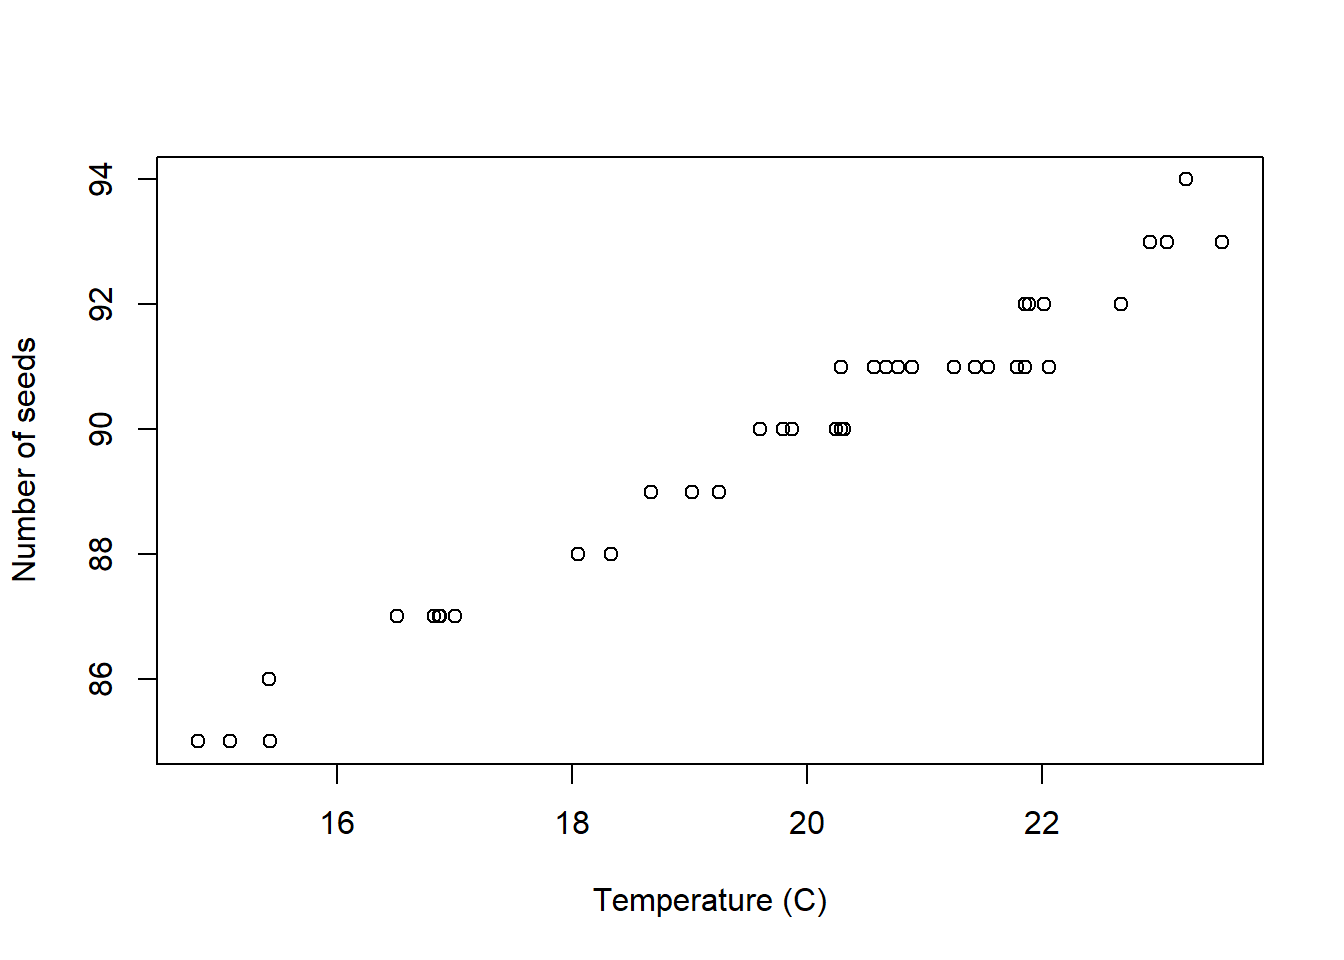
\includegraphics[width=0.7\linewidth]{_main_files/figure-latex/fig-scatterplot1-1} 

}

\caption{Scatter plot of number of seeds versus average temperature (40 observations)}\label{fig:fig-scatterplot1}
\end{figure}

This is very useful for exploring the relationship between two variables. In the above example we observe that the number of seeds which germinate increases linearly with temperature. We can extend the approach to comparing more than two variables by producing
a \textbf{scatterplot matrix}
which consists of scatterplots for every pair of random variables, see
Figure \ref{fig:fig-scatterplot2}.

\begin{figure}

{\centering 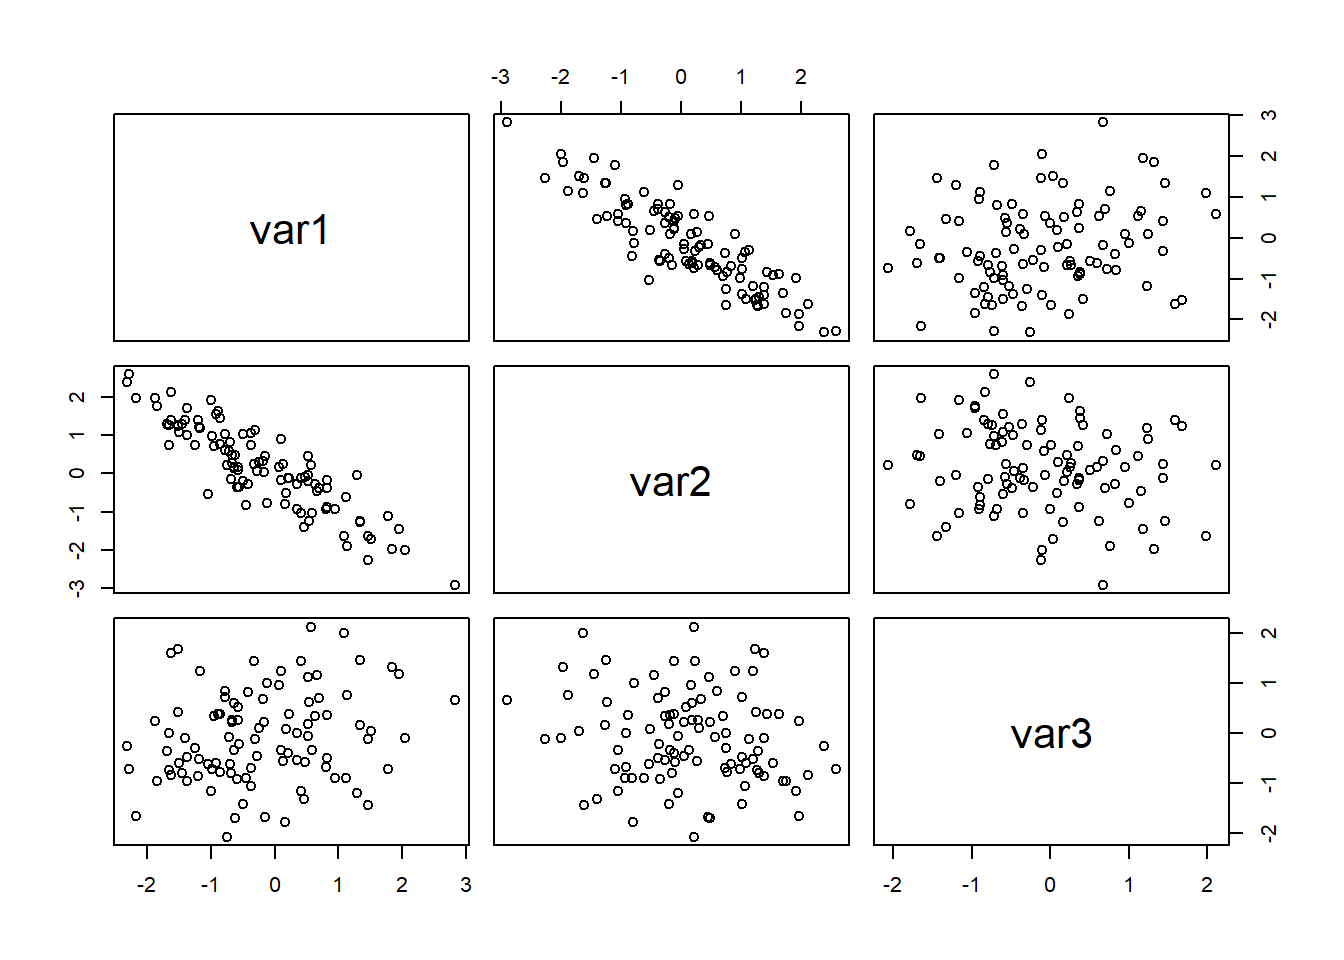
\includegraphics[width=0.95\linewidth]{_main_files/figure-latex/fig-scatterplot2-1} 

}

\caption{A scatterplot matrix for three variables (100 observations)}\label{fig:fig-scatterplot2}
\end{figure}

\hypertarget{visual_plot_summary}{%
\subsection{\texorpdfstring{{\textbf{Summary}}}{Summary}}\label{visual_plot_summary}}

{\textbf{Histogram/Dotplot}}

\emph{Pros:} Gives a good impression of the distribution of the data.

\emph{Cons:} The histogram is sensitive to the classes chosen to group
observations -- giving only a vague impression of the data.

{\textbf{Density plot}}

\emph{Pros:} Represents continuous distribution by a continuous function (density) aoviding the discretisation of histograms.

\emph{Cons:} Over-interprets individual observations for small sample sizes often leading to erroneous multi-modality.

{\textbf{Boxplot}}

\emph{Pros:} Good for comparing different samples or groups of observations on
the same random variable. Gives a good quick summary of the data.

\emph{Cons:} Gives no feel for the number of observations involved. Hides
multiple modes.

{\textbf{Stem and leaf plot}}

\emph{Pros:} Gives indication of general shape and other distributional
features while allowing actual data values to be recovered.

\emph{Cons:} Difficult to use for comparative purposes -- suffers from lack of
clarity.

{\textbf{Pie chart}}

\emph{Pros:} Looks nice.

\emph{Cons:} Only useful for comparing the relative proportions of observations
in a small number of categories. Difficult to compare categories with
similar frequencies, or very small frequencies.

\hypertarget{visual_data}{%
\section{Commenting on data}\label{visual_data}}

When we describe a data set in words, often to complement a plot, here are some things worth commenting about:

\begin{itemize}
\tightlist
\item
  \emph{Location} - what is a typical value?\\
\item
  \emph{Spread} - how dispersed are the observations?\\
\item
  \emph{Multiple modes} - is there one or more `peaks' (and why)?\\
\item
  \emph{Symmetry/skewness} - is skewness positive, negative, roughly zero?\\
\item
  \emph{Outliers} - are there any unusual observations?\\
\item
  \emph{Any other interesting patterns or features} - e.g.~are two variables related?
\end{itemize}

We have given an overview of summarising data, both numerically (location and spread) and graphically. We are now in position to consider the mathematical underpinnings of statistics through the introduction of probability.

\hypertarget{visual:lab}{%
\section*{\texorpdfstring{{\textbf{Task: Session 2}}}{Task: Session 2}}\label{visual:lab}}
\addcontentsline{toc}{section}{{\textbf{Task: Session 2}}}

In \protect\hyperlink{Rmark}{Section 24}, an introduction using to \textbf{R Markdown} is given.

Work through \protect\hyperlink{Rmark}{Section 24} and then attempt to complete the \textbf{R Markdown} file for Session 2:\\
\href{https://moodle.nottingham.ac.uk/course/view.php?id=134982\#section-2}{Session 2: Plots in R}

\hypertarget{prob}{%
\chapter{Probability}\label{prob}}

\hypertarget{prob:overview}{%
\section{Overview}\label{prob:overview}}

In this Chapter we introduce \textbf{probability} as a \textbf{measure} associated with a \textbf{random experiment}. After providing a short motivation for probability (\protect\hyperlink{prob:motivation}{Section 4.2}), we begin in \protect\hyperlink{prob:sample_space}{Section 4.3} with the notion of a \textbf{Sample space} (\protect\hyperlink{prob:sample_space}{Section 4.3}), the set of possible outcomes of a random experiment and \textbf{Events} (\protect\hyperlink{prob:events}{Section 4.4}), the outcome(s) which occur. This enables us in \protect\hyperlink{prob:defn}{Section 4.5} to define \protect\hyperlink{prob:def:prob}{\textbf{probability}} as a finite measure which uses the scale 0 (impossible) to 1 (certain) to define the likelihood of an event. We conclude the chapter by introducing the concept of \protect\hyperlink{prob:def:cond}{\textbf{conditional probability}} (\protect\hyperlink{prob:Conditional_Probability}{Section 4.6}), the probability of one event \textbf{given} (conditional upon) another event (or events) having occurred. We present the key results of the \protect\hyperlink{prob:thm:totalprob}{Theorem of total probability} and \protect\hyperlink{prob:thm:bayes}{Bayes' formula}.
The discussion of conditional probability leads us naturally to consider the dependence between two (or more) events and the notion of \protect\hyperlink{prob:def:independence}{\textbf{independence}}, where the probability of an event occurring is not affected by whether or not another event has occurred and we explore this further in \protect\hyperlink{prob:mutual}{Section 4.7}.

\hypertarget{prob:motivation}{%
\section{Motivation}\label{prob:motivation}}

There are many situations where we have uncertainty and want to quantify that uncertainty.

\begin{enumerate}
\def\labelenumi{(\alph{enumi})}
\tightlist
\item
  Manchester United will win the Premier League this season.\\
\item
  The Labour Party will win the next general election.\\
\item
  The £ will rise against the \$ today.\\
\item
  Coin tossed repeatedly - a head will turn up eventually.\\
\item
  In 5 throws of a dart, I will hit the Bull's eye once.\\
\item
  If I play the lottery every week I will win a prize next year.
\end{enumerate}

(a)-(c) are subjective probabilities, whereas (d)-(f) are objective/statistical/physical probabilities.

The general idea is:

\begin{enumerate}
\def\labelenumi{(\alph{enumi})}
\tightlist
\item
  A conceptual random experiment \(\mathcal{E}\).\\
\item
  List all possible outcomes \(\Omega\) for the experiment \(\mathcal{E}\) but \textbf{don't know} which occurs, has occurred or will occur.\\
\item
  Assign to each possible outcome \(\omega\) a real number which is the probability of that outcome.
\end{enumerate}

\hypertarget{prob:sample_space}{%
\section{Sample Space}\label{prob:sample_space}}

We begin by defining a \emph{set}.

\leavevmode\vadjust pre{\hypertarget{prob:def:set}{}}%
\textcolor{red}{Definition 4.3.1.}
{\textbf{Set.}}\\
A \emph{set} is a collection of objects. The notation for a set is to simply list every object separated by commas, and to surround this list by curly braces \(\{\) and \(\}\). The objects in a set are referred to as the \emph{elements} of the set.

There is no restrictions on what constitutes as an object in set. A set can have a finite or infinite number of elements. The ordering of the elements in a list is irrelevant. Two sets are equal if and only if they have the same collection of elements.

\leavevmode\vadjust pre{\hypertarget{prob:def:samplespace}{}}%
\textcolor{red}{Definition 4.3.2.}
{\textbf{Sample space.}}\\
The \emph{sample space} \(\Omega\) for a random experiment \(\mathcal{E}\) is the set of all possible outcomes of the random experiment.

\leavevmode\vadjust pre{\hypertarget{prob:ex:dice}{}}%
\textcolor{red}{Example 4.3.3.}
{\textbf{Rolling a die.}}

The sample space for the roll of a die is

\[\Omega = \{ 1,2,3,4,5,6 \},\]

that is, the set of the six possible outcomes.

\hfill\break

\leavevmode\vadjust pre{\hypertarget{prob:ex:dart}{}}%
\textcolor{red}{Example 4.3.4.}
{\textbf{Dart in a target.}}

Dart into a circular target, radius 1:

\[\Omega = \{ (x,y): x^2 + y^2 \leq 1\},\]\\

\begin{figure}
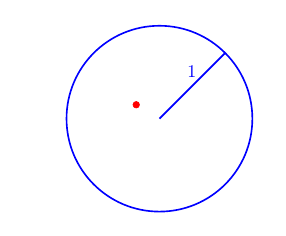
\includegraphics[width=0.8\linewidth]{Images/dart1} \caption{ Example: $(x,y) =(-0.25,0.15)$.}\label{fig:dart1}
\end{figure}

that is, the set of pairs of real numbers that are less than a distance 1 from the origin \((0,0)\).

Note that the examples illustrate how \(\Omega\) may be discrete or continuous.

\hypertarget{prob:events}{%
\section{Events}\label{prob:events}}

\leavevmode\vadjust pre{\hypertarget{prob:def:event}{}}%
\textcolor{red}{Definition 4.4.1.}
{\textbf{Event.}}\\
An \emph{event} relating to an experiment is a subset of \(\Omega\).

\leavevmode\vadjust pre{\hypertarget{prob:ex:twocoins}{}}%
\textcolor{red}{Example 4.4.2.}
{\textbf{Toss two coins.}}

The sample space for the toss of two fair coins is

\[\Omega = \{ HH, HT, TH, TT \}.\]

Let \(A\) be the event that at least one head occurs, then

\[A = \{ HH, HT, TH \}.\]

Note that the events \(HT\) (Head on coin 1 and Tail on coin 2) and \(TH\) (Tail on coin 1 and Head on coin 2) are distinct events.

\hfill\break

\leavevmode\vadjust pre{\hypertarget{prob:ex:volcano}{}}%
\textcolor{red}{Example 4.4.3.}
{\textbf{Volcano eruption.}}

The sample space of time in years until a volcano next erupts is
\[ \Omega = \{t: t >0 \} =(0,\infty),\]
that is, all positive real numbers. Let event \(L\) be the volcano erupting in the next \(10\) years, then
\[L = \{t: 0 < t \leq 10\} =(0,10].\]

We summarise key set notation, involving sets \(E\) and \(F\), below:

\begin{enumerate}
\def\labelenumi{\arabic{enumi}.}
\tightlist
\item
  We use \(\omega \in E\) to denote that \(\omega\) is an element of the set \(E\). Likewise, \(\omega \notin E\) denotes that \(\omega\) is not an element of \(E\);\\
\item
  The notation \(E \subseteq F\) means that if \(\omega \in E\), then \(\omega \in F\). In this case, we say \(E\) is a \emph{subset} of \(F\);\\
\item
  \(E^{c}\) - complement of \(E\), sometimes written \(\bar{E}\).\\
  \(E^{c}\) consists of all points in \(\Omega\) that are not in \(E\). Thus, \(E^{c}\) occurs
  if and only if \(E\) does not occur, see Figure \ref{fig:Set1}.
\end{enumerate}

\begin{figure}
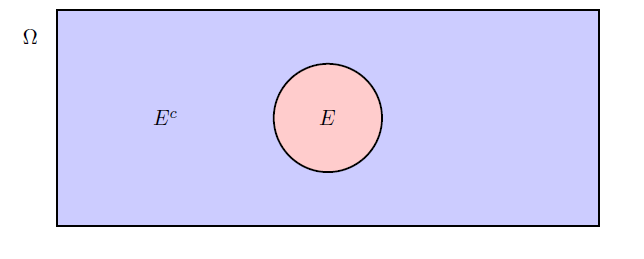
\includegraphics[width=0.8\linewidth]{Images/Set1} \caption{ Complement example.}\label{fig:Set1}
\end{figure}

\begin{enumerate}
\def\labelenumi{\arabic{enumi}.}
\setcounter{enumi}{3}
\tightlist
\item
  The \emph{intersection} of two sets \(E\) and \(F\), denoted \(E \cap F\), is the set of all elements that belong to both \(E\) and \(F\), see Figure \ref{fig:Set2}.
\end{enumerate}

\begin{figure}
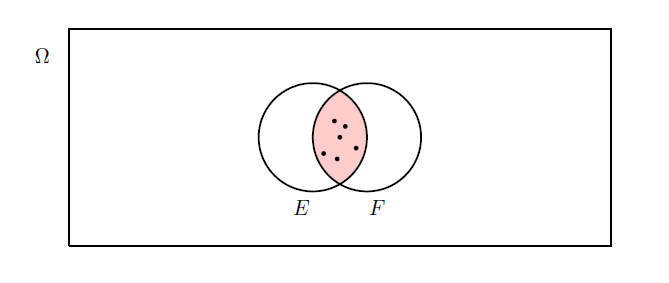
\includegraphics[width=0.8\linewidth]{Images/Set2} \caption{ Intersection example.}\label{fig:Set2}
\end{figure}

\begin{enumerate}
\def\labelenumi{\arabic{enumi}.}
\setcounter{enumi}{4}
\tightlist
\item
  If \(E \cap F = \emptyset\) then \(E\) and \(F\) cannot both occur, \emph{i.e.} \(E\) and \(F\)
  are \emph{disjoint} (or \emph{exclusive}) sets, see Figure \ref{fig:Set3}.
\end{enumerate}

\begin{figure}
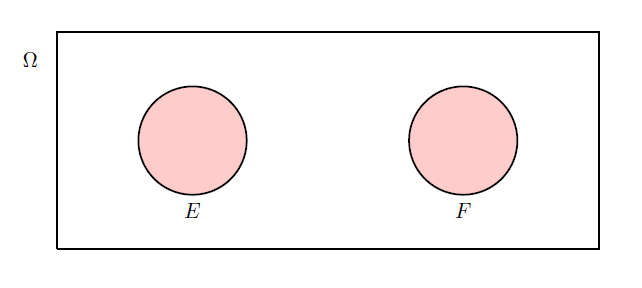
\includegraphics[width=0.8\linewidth]{Images/Set3} \caption{ Disjoint (exclusive) example.}\label{fig:Set3}
\end{figure}

\begin{enumerate}
\def\labelenumi{\arabic{enumi}.}
\setcounter{enumi}{5}
\tightlist
\item
  The \emph{union} of two sets \(E\) and \(F\), denoted \(E \cup F\), is the set of all elements that belong to either \(E\) or to \(F\), see Figure \ref{fig:Set4}.
\end{enumerate}

\begin{figure}
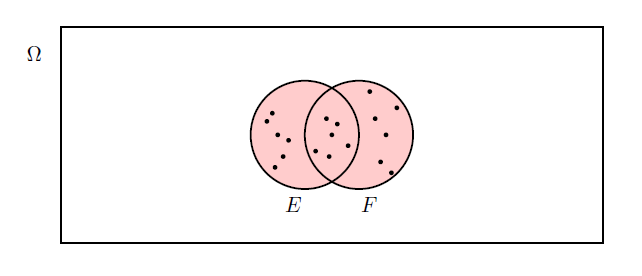
\includegraphics[width=0.8\linewidth]{Images/Set4} \caption{ Union example.}\label{fig:Set4}
\end{figure}

\begin{enumerate}
\def\labelenumi{\arabic{enumi}.}
\setcounter{enumi}{6}
\tightlist
\item
  The set \(\{\}\) with no elements in it is called the \emph{empty set} and is denoted \(\emptyset\).\\
  \textbf{Note}: \(\Omega^c = \emptyset\) and \(\emptyset^c = \Omega\).
\end{enumerate}

A summary of sets notation using the outcomes from a six sided die are presented in the \protect\hyperlink{video6}{Video 6}.

Watch \href{https://mediaspace.nottingham.ac.uk/media/Sets+FINAL+VERSION/1_cigsltq1}{\textcolor{blue}{Video 6: Set notation}}

\hypertarget{prob:defn}{%
\section{Probability}\label{prob:defn}}

There are different possible interpretations of the meaning of a probability:

\begin{itemize}
\item
  \textbf{Classical interpretation.}
  Assuming that all outcomes of an experiment are equally likely, then the probability of an event \(A = \frac{n(A)}{n(\Omega)}\), where \(n(A)\) is the number of outcomes satisfying \(A\) and \(n(\Omega)\) is the number of outcomes in \(\Omega\) (total number of possible outcomes).
\item
  \textbf{Frequency interpretation.}
  The probability of an event is the relative frequency of observing a particular outcome when an experiment is repeated a large number of times under similar circumstances.
\item
  \textbf{Subjective interpretation.}
  The probability of an event is an individual's perception as to the likelihood of an event's occurrence.
\end{itemize}

\leavevmode\vadjust pre{\hypertarget{prob:def:prob}{}}%
\textcolor{red}{Definition 4.5.1.}
{\textbf{Probability.}}

A \emph{probability} (\emph{measure}) is a real-valued set function \(P\) defined on the events (subsets) of a sample space \(\Omega\) satisfying the following three axioms (see Kolmogorov, 1933):

\begin{enumerate}
\def\labelenumi{\arabic{enumi}.}
\tightlist
\item
  \(P(E)\geq0\) for any event \(E\);
\item
  \(P(\Omega)=1\);
\item
  If \(E_1,E_2,\dots, E_n\) are disjoint events (i.e.~\(E_i \cap E_j = \emptyset\) for all \(i \neq j\)), then
  \[P \left( \bigcup_{i=1}^n E_i \right) = \sum_{i=1}^n P(E_i).\]
\end{enumerate}

If \(\Omega\) is \emph{infinite} then 3. can be extended to:\\
3'. If \(E_1,E_2,\dots\) is any infinite sequence of disjoint events (i.e.~\(E_i \cap E_j = \emptyset\) for all \(i\not=j\)), then
\[P \left( \bigcup_{i=1}^\infty E_i \right) = \sum_{i=1}^\infty P(E_i).\]

Note that all of the other standard properties of probability (measures) that we use are derived from these three axioms.

\leavevmode\vadjust pre{\hypertarget{prob:exer:1}{}}%
\textcolor{red}{Example 4.5.2.}\\
Using only the axioms above, prove:

\begin{itemize}
\item
  \(0 \leq P(E) \leq 1\) for any event \(E\);
\item
  \(P(E^C) = 1 - P(E)\) where \(E^C\) is the complement of \(E\);
\item
  \(P(\emptyset) = 0\);
\item
  \(P(A \cup B) = P(A) + P(B) - P(A \cap B)\).\\
\end{itemize}

A summary of probability along with proofs of the results in \protect\hyperlink{prob:exer:1}{Example 4.5.2} are provided in \protect\hyperlink{video7}{Video 7}.

Watch \href{https://mediaspace.nottingham.ac.uk/media/Probability+FINAL+VERSION/1_43tb6qxp}{\textcolor{blue}{Video 7: Probability}}

Solution to Example 4.5.2.

Since for any event \(E\), \(\Omega = E \cup E^c\), we have by axiom 2 that

\[ 1 = P (\Omega) = P (E \cup E^c).  \]

By axiom 3, since \(E\) and \(E^c\) are disjoint events, we have that

\[ 1 = P (E \cup E^c)= P (E) + P (E^c).  \]

which rearranges to give \(P(E^c) = 1-P(E)\).

\textbf{Special cases}\\
If \(E = \emptyset\), then \(E^c = \Omega\) giving \(1 = P(\emptyset) +1\) and it follows that \(P(\emptyset)=0\).\\
Since \(P(E^c) \geq 0\), we have that \(P(E) \leq 1\) and hence \(0\leq P(E) \leq 1\).

To study \(P(A \cup B)\), we note that \(A \cup B\) is formed by the union of the disjoint events: \(A \cap B^c\), \(A \cap B\) and \(A^c \cap B\). Therefore using axiom 3,

\[ P(A \cup B) = P(A \cap B^c) + P(A \cap B)+P(A^c \cap B).   \]

Similarly, we have that

\[ P(A) = P(A \cap B^c) + P(A \cap B)\]

and

\[ P(B) =P(A \cap B)+P(A^c \cap B).\]

Since \(P(A^c \cap B) = P(B)-P(A \cap B)\), we have that

\begin{eqnarray*} P(A \cup B) &=& P(A \cap B^c) + P(A \cap B) + P(A^c \cap B)  \\
&=& P(A) + P(B)-P(A \cap B)   \\
&=& P(A) + P(B)-P(A \cap B).
\end{eqnarray*}

\hfill\break

In many cases, \(\Omega\) consists of \(N (=n(\Omega))\) equally likely elements, \emph{i.e.}
\[
\Omega = \left\{ \omega_{1}, \omega_{2}, \ldots, \omega_{N} \right\}, 
\]
with \(P(\omega_i) = \frac{1}{N}\).

Then, for any event \(E\) (\emph{i.e.} subset of \(\Omega\)),
\[
P(E) = \frac{n(E)}{n(\Omega)} = \frac{n(E)}{N}
\]
coinciding with the Classical interpretation of probability.

\leavevmode\vadjust pre{\hypertarget{prob:ex:class}{}}%
\textcolor{red}{Example 4.5.3.}\\
1. {\textbf{Throw a die.}} \(\Omega = \left\{ 1,2,3,4,5,6 \right\}\).
\[ P(\{1\})=P(\{2\})= \ldots = P(\{6\})= \frac{1}{6}. \]
The probability of throwing an odd number is
\[P(\mbox{Odd}) = P( \left\{ 1,3,5 \right\}) = \frac{3}{6} = \frac{1}{2}. \]\\
2. {\textbf{Draw a card at random from a standard pack of 52.}}
\[\Omega = \left\{ A\clubsuit, 2\clubsuit, 3\clubsuit, \ldots, K\diamondsuit \right\}. \]
\(P(\omega) = 1/52\) for all \(\omega \in \Omega\).\\
If \(E = \left\{ \mbox{Black} \right\}\) and \(F = \left\{ \mbox{King} \right\}\),
then there are 26 black cards, \(n(E) =26\), 4 kings, \(n(F)=4\) and 2 black kings (\(K\clubsuit\) and \(K\spadesuit\)), \(n(E\cap F)=2\),
\begin{eqnarray*}
P(E \cup F) & = & P(E) + P(F) - P(E \cap F) \\
& = & \frac{26}{52} + \frac{4}{52} - \frac{2}{52} \\
& = & \frac{7}{13}.
\end{eqnarray*}

\hypertarget{prob:Conditional_Probability}{%
\section{Conditional probability}\label{prob:Conditional_Probability}}

\leavevmode\vadjust pre{\hypertarget{prob:def:cond}{}}%
\textcolor{red}{Definition 4.6.1.}
{\textbf{Conditional Probability.}}

The \emph{conditional probability} of an event \(E\) \emph{given} an event \(F\) is

\[P(E\mid F)=\frac{P(E\cap F)}{P(F)},\quad \mbox{ provided } P(F)>0.\]

Note if \(P(F)>0\), then \(P(E \cap F) = P(E|F) P(F)\).

Moreover, since \(E \cap F = F \cap E\), we have that
\[ P(E|F) P(F) = P(E \cap F) = P (F \cap E) = P(F|E) P(E).   \]
In other words, to compute the probability of both events \(E\) and \(F\) occurring, we can either:

\begin{itemize}
\tightlist
\item
  Consider first whether \(E\) occurs, \(P(E)\), and then whether \(F\) occurs \emph{given} that \(E\) has occurred, \(P(F|E)\),\\
\item
  Or consider first whether \(F\) occurs, \(P(F)\), and then whether \(E\) occurs \emph{given} that \(F\) has occurred, \(P(E|F)\).
\end{itemize}

\leavevmode\vadjust pre{\hypertarget{prob:ex:dice2}{}}%
\textcolor{red}{Example 4.6.2.}
{\textbf{Rolling a die.}}

Consider the experiment of tossing a fair 6-sided die. What is the probability of observing a 2 if the outcome was even?

Let event \(T\) be observing a 2 and let event \(E\) be the outcome is even. Find \(P(T|E)\):

\[P(T|E)=\frac{P(T \cap E)}{P(E)} = \frac{1/6}{1/2} = \frac{1}{3}.\]

\leavevmode\vadjust pre{\hypertarget{prob:def:independence}{}}%
\textcolor{red}{Definition 4.6.3.}
{\textbf{Independence.}}

Two events \(E\) and \(F\) are independent if

\[P(E\cap F)=P(E)P(F).\]

\leavevmode\vadjust pre{\hypertarget{prob:thm:independence}{}}%
\textcolor{red}{Theorem 4.6.4.}\\
If \(P(F)>0\), two events, \(E\) and \(F\), are independent if and only if \(P(E|F)=P(E)\).

\begin{align*}
& P(E|F) = P(E) \\
\iff \quad & \frac{P(E \cap F)}{P(F)} = P(E) \\
\iff \quad & P(E \cap F) = P(E)P(F) \\
\iff \quad & E \text{ and } F \text{ are independent.}
\end{align*}

\hfill\break

\textbf{Observations on Independence}

\begin{itemize}
\tightlist
\item
  If \(E\) and \(F\) are \textbf{NOT} independent then
  \[
  P( E \cap F) \neq P(E)P (F).
  \]\\
\item
  \(E\) and \(F\) being independent is \textbf{NOT} the same as \(E\) and \(F\) being disjoint.
\end{itemize}

\textbf{Independence:} \(P( E \cap F) = P(E)P(F)\).\\
\textbf{Disjoint (exclusive):} \(P( E \cap F) = P (\emptyset) = 0\).

\leavevmode\vadjust pre{\hypertarget{prob:ex:dice3}{}}%
\textcolor{red}{Example 4.6.5.}
{\textbf{Rolling a die.}}

Consider the experiment of tossing a fair 6-sided die.\\
Let \(E= \{2,4,6\}\), an even number is rolled on the die and \(F= \{3,6\}\), a multiple of 3 is rolled on the die.

Are \(E\) and \(F\) independent?

\(E \cap F = \{6 \}\), so \(P(E \cap F) = \frac{1}{6}\).\\

\[P(E) \times P(F) = \frac{3}{6} \times \frac{2}{6} = \frac{1}{6} = P(E \cap F) \]

Therefore \(E\) and \(F\) are independent.

\leavevmode\vadjust pre{\hypertarget{prob:partition}{}}%
\textcolor{red}{Definition 4.6.6.}
{\textbf{Partition.}}

A \emph{partition} of a sample space \(\Omega\) is a collection of events \(E_{1}, E_{2}, \ldots,E_n\) in \(\Omega\) such that:

\begin{enumerate}
\def\labelenumi{\roman{enumi}.}
\tightlist
\item
  \(E_{i} \cap E_{j} = \emptyset\) for all \(i \neq j\) (disjoint sets)\\
\item
  \(E_{1} \cup E_{2} \cup \ldots \cup E_n \; = \bigcup_{i=1}^n E_i = \Omega\).\\
\end{enumerate}

We can set \(n=\infty\) in \protect\hyperlink{prob:partition}{Definition 4.6.6} and have infinitely many events constructed the partition.

Figure \ref{fig:partition1} presents an example of a partition of \(\Omega\) using six events
\(E_1,E_2, \ldots, E_6\).

\begin{figure}
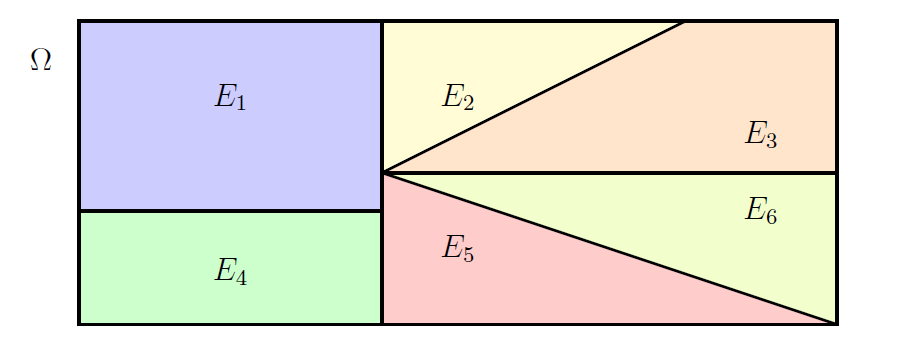
\includegraphics[width=0.8\linewidth]{Images/partition1} \caption{Example of a partition of a sample space using six events.}\label{fig:partition1}
\end{figure}

For an event \(F \subseteq \Omega\),

\[ F = (F \cap E_1) \cup (F \cap E_2 ) \cup \ldots \cup (F \cap E_n ). \]

This is illustrated in Figure \ref{fig:partition2} using the partition given in Figure \ref{fig:partition1}.

\begin{figure}
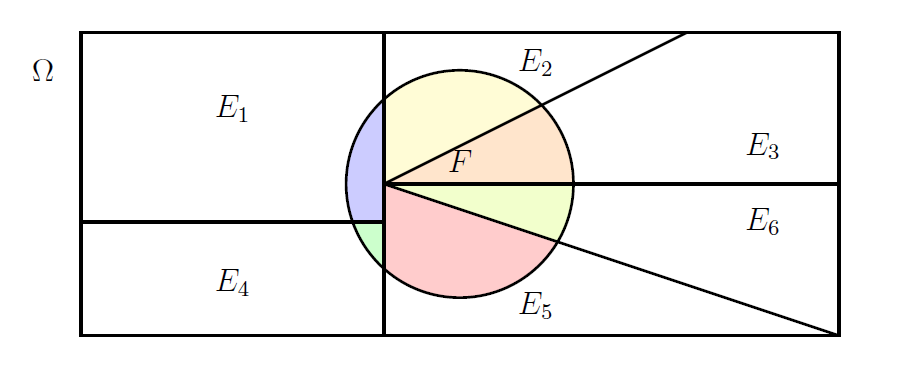
\includegraphics[width=0.8\linewidth]{Images/partition2} \caption{The event *F* expressed in terms of the union of events.}\label{fig:partition2}
\end{figure}

\leavevmode\vadjust pre{\hypertarget{prob:thm:totalprob}{}}%
\textcolor{red}{Theorem 4.6.7.}
{\textbf{Theorem of Total Probability.}}

Let \(E_1,E_2,\dots, E_n\) be a partition of \(\Omega\) (i.e.~\(E_i\cap E_j=\emptyset\) for all \(i\not=j\) and \(\bigcup\limits_{i=1}^n E_i=\Omega\)) and let \(F\subseteq \Omega\) be any event. Then,

\[P(F)=\sum_{i=1}^n P(F\mid E_i)\,P(E_i).\]

\leavevmode\vadjust pre{\hypertarget{prob:prf:totalprob}{}}%
Since the \(E_i\)'s form a partition:

\begin{enumerate}
\def\labelenumi{\arabic{enumi}.}
\tightlist
\item
  \(F = F \cap \Omega = \bigcup_{i=1}^n [ F \cap E_i ]\).\\
\item
  For each \(i \neq j\), \([F \cap E_i] \cap [F \cap E_j] = \emptyset\).
\end{enumerate}

Therefore

\begin{eqnarray} 
P(F) = \sum_{i=1}^n P \left(F \cap E_i \right).  
\label{eq:pp1}  
\end{eqnarray}

By the definition of conditional probability, for each \(i\),\\

\begin{equation} 
P\left(F \cap E_i \right) = P(F|E_i) P(E_i).  
\label{eq:pp2}  
\end{equation}

Substituting \eqref{eq:pp2} into \eqref{eq:pp1} completes the proof.

\leavevmode\vadjust pre{\hypertarget{prob:ex:factory}{}}%
\textcolor{red}{Example 4.6.8.}
{\textbf{Tin can factory.}}

Suppose that a factory uses three different machines to produce tin cans. Machine I produces 50\% of all cans, machine II produces 30\% of all cans and machine III produces the rest of the cans. It is known that 4\% of cans produced on machine I are defective, 2\% of the cans produced on machine II are defective and 5\% of the cans produced on machine III are defective. If a can is selected at random, what is the probability that it is defective?

Let event \(M_i\) be the can is produced by machine \(i\), \(i=1,2,3\). Let \(D\) be the event that the can is defective. From the question, we know

\begin{eqnarray*}
P(M_1) &=& 0.5, \qquad P(D|M_1) = 0.04,\\
P(M_2) &=& 0.3, \qquad P(D|M_2) = 0.02,\\
P(M_3) &=& 0.2, \qquad P(D|M_3) = 0.05.\\
\end{eqnarray*}

Therefore\\

\begin{eqnarray*}
P(D) &=& \sum_{i=1}^3 P(D|M_i)P(M_i)\\
&=& (0.04 \times 0.5) + (0.02 \times 0.3) + (0.05 \times 0.2) \\
&=& 0.036.
\end{eqnarray*}

\hfill\break

\leavevmode\vadjust pre{\hypertarget{prob:job_interview}{}}%
\textcolor{red}{Example 4.6.9.}
{\textbf{Job interview problem.}}

A manager interviews 4 candidates for a job. The manager \textbf{MUST} make a decision offer/reject
after each interview. Suppose that candidates are ranked \(1,2,3,4\) (1 best) and are
interviewed in random order.

The manager interviews and rejects the first candidate. They then offer the job to
the first candidate that is better than the rejected candidate. If all are worse
then they offer the job to the last candidate.

What is the probability that the job is offered to the best candidate?

Attempt \protect\hyperlink{prob:job_interview}{Example 4.6.9 (Job interview problem)} and then watch \protect\hyperlink{video8}{Video 8} for the solution.

Watch \href{https://mediaspace.nottingham.ac.uk/media/Job+Interview+FINAL+VERSION/1_nzxxre7o}{\textcolor{blue}{Video 8: Job Interview}}

Solution to Example 4.6.9 (Job interview problem).

Let \(F\) be the event that the best candidate is offered the job.

For \(k=1,2,3,4\), let \(E_k\) be the event that candidate \(k\) (the \(k^{th}\) best candidate) is interviewed first. Note that \(E_k\)s form a partition of the sample space and by randomness,

\[ P(E_1) = P(E_2)=P(E_3)=P(E_4) = \frac{1}{4}. \]

We have that:\\
1. \(P(F|E_1) =0\). If the \(1^{st}\) ranked candidate is interviewed first they will be rejected and cannot be offered the job.\\
2. \(P(F|E_2) =1\). If the \(2^{nd}\) ranked candidate is interviewed first then all candidates will be rejected until the best (\(1^{st}\) ranked) candidate is interviewed and offered the job.\\
3. \(P(F|E_3) =\frac{1}{2}\). If the \(3^{rd}\) ranked candidate is interviewed first then whoever is interviewed first out of the \(1^{st}\) ranked and \(2^{nd}\) ranked candidates will be offered the job. Each of these possibilities is equally likely.\\
4. \(P(F|E_4) =\frac{1}{3}\). If the \(4^{th}\) ranked (worst) candidate is interviewed first then the \(1^{st}\) ranked candidate will only be offered the job if they are interviewed second.

By the Theorem of Total Probability,

\begin{eqnarray*}
P(F) &=& \sum_{i=1}^4 P(F|E_i) P(E_i) \\
&=& P(F |E_1) P(E_1) + P(F |E_2) P(E_2) + P(F |E_3) P(E_3) + P(F |E_4) P(E_4)   \\
&=& 0 \times \frac{1}{4} + 1 \times \frac{1}{4} + \frac{1}{2} \times \frac{1}{4}+ \frac{1}{3} \times \frac{1}{4} \\
&=& \frac{11}{24}.
\end{eqnarray*}

\hfill\break

\leavevmode\vadjust pre{\hypertarget{prob:thm:bayes}{}}%
\textcolor{red}{Theorem 4.6.10.}
{\textbf{Bayes Formula.}}

Let \(E_1,E_2,\dots,E_n\) be a partition of \(\Omega\), \emph{i.e.} \(E_i \cap E_j = \emptyset\) for all \(i \not= j\) and \(\bigcup\limits_{i=1}^n E_i=\Omega\), such that \(P(E_i)>0\) for all \(i=1,\dots,n\), and let \(F\subseteq\Omega\) be any event such that \(P(F)>0\). Then\\

\[ P(E_k|F) = \frac{P(F|E_k) P(E_k)}{\sum_{i=1}^n P(F|E_i) P(E_i)}.\]

\hypertarget{prob:prf:bayes}{}
If \(P(F)>0\) and \(P(E_k)>0\), then by definition\\

\[P(E_k|F) = \frac{P(E_k \cap F)}{P(F)} = \frac{P(F|E_k) P(E_k)}{P(F)}.\]

Since \(E_1,E_2,\dots,E_n\) is a partition of \(\Omega\) such that \(P(E_i)>0\) for all \(i\), then by the \protect\hyperlink{prob:thm:totalprob}{Theorem of Total Probability} we can rewrite \(P(F)\) and obtain\\

\[P(E_k|F) = \frac{P(F|E_k) P(E_k)}{\sum_{i=1}^n P(F|E_i) P(E_i)}.\]

\leavevmode\vadjust pre{\hypertarget{prob:ex:factory2}{}}%
\textcolor{red}{Example 6.11.}
{\textbf{Tin can factory (continued).}}

Consider \protect\hyperlink{prob:ex:factory}{Example 4.6.8}. Suppose now that we randomly select a can and find that it is defective.

What is the probability that it was produced by machine I?

\[P(M_1|D)=\frac{P(D|M_1)P(M_1)}{P(D)}=\frac{0.04 \times 0.5}{0.036}=0.55.\]

\leavevmode\vadjust pre{\hypertarget{prob:exer:guilty}{}}%
\textcolor{red}{Example 4.6.12.}
{\textbf{Guilty?}}

At a certain stage of a jury trial a jury member gauges that the probability
that the defendant is guilty is \(7/10\).

The prosecution then produces evidence that fibres of the victim's clothing
were found on the defendant.

If the probability of such fibres being found is 1 if the defendant is guilty and
\(1/4\) if the defendant is not guilty, what now should be the jury member's
probability that the defendant is guilty?

Attempt \protect\hyperlink{prob:exer:guilty}{Example 4.6.12 (Guilty?)} and then watch \protect\hyperlink{video9}{Video 9} for the solution.

Watch \href{https://mediaspace.nottingham.ac.uk/media/GuiltyF+FINAL+VERSION/1_e1qr70ho}{\textcolor{blue}{Video 9: Guilty?}}

Solution to Example 4.6.12 (Guilty?)

Let \(G\) be the event that the defendant is guilty and let \(F\) be the event that fibres are found on the victim's clothing.

We want \(P(G|F)\), the probability of being guilty \textbf{given} fibres are found on the victim's clothing.

We have that \(P(G)=0.7\), \(P(G^c) = 1- P(G)=0.3\), \(P(F|G)=1\) and \(P(F|G^c)=0.25\).

Therefore, by Bayes' Theorem,\\

\begin{eqnarray*}
P(G|F) &=& \frac{P(F \cap G)}{P(F)}  \\ &=& \frac{P(F|G) P(G)}{P(F|G) P(G) + P(F|G^c) P(G^c)}  \\
&=& \frac{1 \times 0.7}{1 \times 0.7 + 0.25 \times 0.3}  \\
&=& 0.9032.
\end{eqnarray*}

\hfill\break

\hypertarget{prob:mutual}{%
\section{Mutual Independence}\label{prob:mutual}}

We can extend the concept of \protect\hyperlink{prob:def:independence}{independence} from two events to \(N\) events.

\leavevmode\vadjust pre{\hypertarget{prob:def:mutual}{}}%
\textcolor{red}{Definition 4.7.1.}
{\textbf{Mutual independence.}}

Events \(E_1,E_2,\dots,E_N\) are (mutually) \emph{independent} if for \emph{any} finite subset \(\{i_1,i_2,\dots,i_n\} \subseteq \{1,\dots,N\}\),\\

\[P\left(\bigcap_{j=1}^nE_{i_j}\right)=\prod_{j=1}^nP(E_{i_j}).\]

\hfill\break

Note, in particular, two events \(E\) and \(F\) are independent if

\[P(E\cap F)=P(E)P(F)\]

\leavevmode\vadjust pre{\hypertarget{prob:aircraft}{}}%
\textcolor{red}{Example 4.7.2.}
{\textbf{Aircraft safety.}}

An aircraft safety system contains \(n\) independent components. The aircraft can fly provided at least one of the components is working. The probability
that the \(i\)th component works is \(p_{i}\). Then\\

\begin{eqnarray*}
P(\mbox{Aircraft can fly}) 
& = & 1 - P( \mbox{Aircraft cannot fly}) \\
& = & 1 - P( \mbox{All components fail}) \\
& = & 1 - \prod_{i=1}^{n} P( \mbox{Component $i$ fails} ) \\
& = & 1 - \prod_{i=1}^{n} (1 - p_{i}).
\end{eqnarray*}

\hfill\break

\hypertarget{rv:lab}{%
\section*{\texorpdfstring{{\textbf{Task: Session 3}}}{Task: Session 3}}\label{rv:lab}}
\addcontentsline{toc}{section}{{\textbf{Task: Session 3}}}

Attempt the \textbf{R Markdown} file for Session 3:\\
\href{https://moodle.nottingham.ac.uk/course/view.php?id=134982\#section-2}{Session 3: Probability in R}

\hypertarget{prob:stud}{%
\section*{\texorpdfstring{{\textbf{Student Exercises}}}{Student Exercises}}\label{prob:stud}}
\addcontentsline{toc}{section}{{\textbf{Student Exercises}}}

Attempt the exercises below.

\leavevmode\vadjust pre{\hypertarget{exer4:1}{}}%
\textcolor{red}{Exercise 4.1.}\\
A card is drawn from a standard pack of 52. Let \(B\) be the event `the card is black', \(NA\) the event `the card is not an Ace' and \(H\) the event `the card is a Heart'. Calculate the following probabilities:

\begin{enumerate}
\def\labelenumi{(\alph{enumi})}
\tightlist
\item
  \(P(B|NA)\);\\
\item
  \(P(NA|B^c)\);\\
\item
  \(P(B^c \cap H | NA)\);\\
\item
  \(P(NA \cup B | H^c)\);\\
\item
  \(P(NA \cup H | NA \cap B)\).\\
\end{enumerate}

\leavevmode\vadjust pre{\hypertarget{exer4:2}{}}%
\textcolor{red}{Exercise 4.2.}\\
A diagnostic test has a probability \(0.95\) of giving a positive result when
applied to a person suffering from a certain disease, and a probability \(0.10\) of giving
a (false) positive when applied to a non-sufferer. It is estimated that \(0.5\%\) of the population
are sufferers. Suppose that the test is applied to a person chosen at random from
the population. Find the probabilities of the following events.

\begin{enumerate}
\def\labelenumi{(\alph{enumi})}
\tightlist
\item
  the test result will be positive.\\
\item
  the person is a sufferer, given a positive result.\\
\item
  the person is a non-sufferer, given a negative result.\\
\item
  the person is missclassified.
\end{enumerate}

\leavevmode\vadjust pre{\hypertarget{exer4:3}{}}%
\textcolor{red}{Exercise 4.3.}\\
In areas such as market research, medical research, etc, it is often hard to get people to
answer embarrassing questions. One way around this is the following. Suppose that \(N\) people
are interviewed, where \(N\) is even. Each person is given a card, chosen at random from \(N\)
cards, containing a single question. Half of the cards contain the embarrassing question, to
which the answer is either `Yes' or `No'. The other half of the cards contain the question `Is your
birthday between January and June inclusive?'

Suppose that of the \(N\) people interviewed, \(R\) answer `Yes' to the question that they received.
Let \(Y\) be the event that a person gives a `Yes' answer, \(E\) the event that they received a card
asking the embarrassing question. Assuming that half the population have birthdays between
January and June inclusive, write down:

\begin{enumerate}
\def\labelenumi{(\alph{enumi})}
\tightlist
\item
  \(P(Y)\);\\
\item
  \(P(E)\);\\
\item
  \(P(Y|E^c)\).
\end{enumerate}

Hence calculate the proportion of people who answered `Yes' to the embarrassing question.

\emph{Hint: Try writing down an expression for \(P(Y)\) using the Theorem of Total Probability.}

Comment on your answer.

\hypertarget{rv}{%
\chapter{Random Variables}\label{rv}}

\hypertarget{rv:overview}{%
\section{Overview}\label{rv:overview}}

In this Chapter we will introduce the concept of a \textbf{random variable} (\protect\hyperlink{rv:des}{Section 5.2}). Random variables assign numerical values to outcomes from a sample space and these can be discrete (counts), continuous (measurements on the real-line) or mixed. Key summaries for random variables are their expectation (mean) and variance, concepts that we have already seen for summarising data and which in \protect\hyperlink{rv:expect}{Section 5.3} we formalise for random variables. We introduce important classes of random variables (probability distributions), both discrete and continuous distributions. These include:

\begin{itemize}
\tightlist
\item
  \protect\hyperlink{rv:Bernoulli}{Section 5.4} Bernoulli random variables and their extensions such as the \protect\hyperlink{rv:Bernoulli:bern}{Bernoulli}, \protect\hyperlink{rv:Bernoulli:bin}{Binomial}, \protect\hyperlink{rv:Bernoulli:geom}{Geometric} and \protect\hyperlink{rv:Bernoulli:negbin}{Negative Binomial} distributions\\
\item
  \protect\hyperlink{rv:Poisson}{Section 5.5} Poisson distribution\\
\item
  \protect\hyperlink{rv:exponential}{Section 5.6} Exponential random variables and their extensions such as the \protect\hyperlink{rv:exponential:exp}{Exponential}, \protect\hyperlink{rv:exponential:gamma}{Gamma}, \protect\hyperlink{rv:exponential:chi}{Chi-squared} and \protect\hyperlink{rv:exponential:beta}{Beta} distributions\\
\item
  \protect\hyperlink{rv:normal}{Section 5.7} Normal (Gaussian) distribution
\end{itemize}

\hypertarget{rv:des}{%
\section{Random variables}\label{rv:des}}

\leavevmode\vadjust pre{\hypertarget{rv:def:rv}{}}%
\textcolor{red}{Definition 5.2.1.}
{\textbf{Random variable.}}

A \emph{random variable} (r.v.) \(X\) is a mapping from \(\Omega\) to \(\mathbb R\), that is

\[X:\Omega \longrightarrow \mathbb{R}.\]

For example,

\begin{itemize}
\item
  Let \(X\) be the number of heads observed when tossing a fair coin three times.
\item
  Let \(T\) be the length of time you wait to be serviced by a bank teller.
\end{itemize}

\textbf{Note:} Random variables can be either discrete (\emph{i.e.} take a finite or countable number of values), continuous, or mixed.

An example of a mixed random variable is, \(R\), the amount of rain \((ml)\) on a given day.

\leavevmode\vadjust pre{\hypertarget{rv:def:cdf}{}}%
\textcolor{red}{Definition 5.2.2.}
{\textbf{Cumulative distribution function.}}

The \emph{cumulative distribution function} (c.d.f.) of a random variable \(X\) is

\[F_X(x) = P(X \leq x) = P(\{\omega\in\Omega:X(\omega)\leq x\}).\]

Properties of the c.d.f include

\begin{itemize}
\item
  \(P(X>x) = 1 - F_X(x)\).
\item
  \(P(x_1 < X \leq x_2) = F_X(x_2) - F_X(x_1)\).
\end{itemize}

Note the c.d.f. is defined for all random variables regardless of whether they are discrete, continuous or mixed.

\leavevmode\vadjust pre{\hypertarget{rv:def:pmf}{}}%
\textcolor{red}{Definition 5.2.3.}
{\textbf{Probability mass function.}}

If \(X\) is a \textbf{discrete} random variable, then we can define a function \(p_X(x)\), called the \emph{probability mass function} (p.m.f.) such that\\

\[p_X(x_i) = P(X=x_i) = P(\{\omega:X(\omega)=x_i\}).\]

\leavevmode\vadjust pre{\hypertarget{rv:ex:coin}{}}%
\textcolor{red}{Example 5.2.4.}
{\textbf{Coin toss.}}

Let \(X\) be the number of heads observed when tossing a fair coin three times. What is the p.m.f. of \(X\)?

\[ p_X(x) = \begin{cases}
1/8, \qquad \text{if $x=0$}, \\
3/8, \qquad \text{if $x=1$}, \\
3/8, \qquad \text{if $x=2$}, \\
1/8, \qquad \text{if $x=3$}, \\
0, \qquad \text{otherwise.}
\end{cases}\]

\leavevmode\vadjust pre{\hypertarget{rv:def:pdf}{}}%
\textcolor{red}{Definition 5.2.5.}
{\textbf{Probability density function.}}

Let \(X\) be a \textbf{continuous} random variable. If there exists some non-negative function \(f_X\) on \(\mathbb R\) such that for any interval \(I\),\\

\[P(X \in I) = \int_I f_X(u) du,\]

the function \(f_X\) is called the \emph{probability density function} (p.d.f.) of \(X\).

Note that if \(F_X(x)\) is the c.d.f. of a continuous random variable \(X\), then the p.d.f. of \(X\) is given by
\[f_X(x) = \frac{d F_X(x)}{dx}.\]

Note that\\

\[ F_X(x) = P(X \leq x) = \begin{cases}
\sum\limits_{x_i \leq x} p_X(x_i), \qquad \text{if $X$ is discrete,} \\[9pt]
\int_{-\infty}^x f_X(u)du, \qquad \text{if $X$ is continuous.}
\end{cases} \]

\hypertarget{rv:expect}{%
\section{Expectation}\label{rv:expect}}

In this Section we formally define the \protect\hyperlink{rv:def:expect}{expectation} (mean), \protect\hyperlink{rv:def:variance}{variance}, \protect\hyperlink{rv:def:median}{median} and \protect\hyperlink{rv:def:mode}{mode} of a random variable. We can note the similarities with the definitions of the \protect\hyperlink{summary_location}{measures of location} (mean, median and mode) and \protect\hyperlink{summary_spread}{variance} of summary statistics in \protect\hyperlink{summary}{Section 2}.

\leavevmode\vadjust pre{\hypertarget{rv:def:expect}{}}%
\textcolor{red}{Definition 5.3.1.}
{\textbf{Expectation.}}

The \emph{expectation} of a random variable \(X\) is defined by\\

\[E[X] = \begin{cases}
\sum\limits_{x_i} x_i p_X(x_i), \quad \text{if $X$ is discrete,} \\[9pt]
\int_{-\infty}^\infty x f_X(x)dx, \quad \text{if $X$ is continuous.}
\end{cases}\]

Note that \(E[X]\) only exists if \(E[|X|]<\infty\) and that \(E[X]\) is a measure of the \emph{centre} of the distribution, that is the centre of mass. We can also define expectations of functions of random variables.

\hypertarget{rv:def:expect2}{}
\textcolor{red}{Definition 5.3.2.}\\
If \(Y=g(X)\) then the \emph{expectation} of \(Y\) is given by\\

\begin{align*}
E[Y] &= E[g(X)] 
&= \begin{cases}
\sum\limits_{x_i} g(x_i) p_X(x_i), \quad \text{if $X$ is discrete,} \\[9pt]
\int_{-\infty}^\infty g(x) f_X(x) \,dx, \quad \text{if $X$ is continuous.}
\end{cases}
\end{align*}

For constants \(c\), \(c_i\) and \(d\), the following are properties of the expectation:

\begin{itemize}
\tightlist
\item
  \(E[c]=c\);\\
\item
  \(E[c g(X) + d]= c E[g(X)] + d\);\\
\item
  \(E \left[ \sum\limits_{i=1}^n c_i g_i(X_i) \right] = \sum\limits_{i=1}^n c_i E[g_i(X_i)]\);\\
\item
  A special case of the above results is \(c_1 = \ldots =c_n =1\) and \(g_i (\cdot)\) is the identity transform, \(g_i (X_i) =X_i\). Then \(E \left[ \sum\limits_{i=1}^n X_i \right] = \sum\limits_{i=1}^n E \left[ X_i \right]\).
\end{itemize}

\leavevmode\vadjust pre{\hypertarget{rv:def:variance}{}}%
\textcolor{red}{Definition 5.3.3.}
{\textbf{Variance.}}

The \emph{variance} of \(X\) is

\[ \text{Var} (X) = E \left[ (X-E[X])^2 \right].\]

The \emph{standard deviation} of \(X\) is \(\sqrt{\text{Var} (X)}\).

For constants \(c\), \(c_i\) and \(d\), the following are properties of the variance:

\begin{itemize}
\item
  \(\text{Var}(X) = E[X^2] - (E[X])^2\);
\item
  \(\text{Var}(X) \geq 0\);
\item
  \(\text{Var}(cX + d) = c^2 \text{Var}(X)\);
\item
  If \(X_1,\dots,X_n\) are independent, then\\

  \[\text{Var} \left( \sum_{i=1}^n c_i X_i \right) = \sum_{i=1}^n c_i^2 \text{Var} (X_i).\]
\end{itemize}

\leavevmode\vadjust pre{\hypertarget{rv:def:median}{}}%
\textcolor{red}{Definition 5.3.4.}
{\textbf{Median.}}

The \emph{median} of \(X\) is defined as \(x_{0}\) such that \(F_X (x_{0}) =0.5\).

For a discrete random variable it is unlikely that there exists \(x_0\) such that \(F_X (x_{0}) =0.5\). Therefore for discrete random variables the median is defined to be the smallest \(x_0\) such that \(F_X (x_0) \geq 0.5\).

\leavevmode\vadjust pre{\hypertarget{rv:def:mode}{}}%
\textcolor{red}{Definition 5.3.5.}
{\textbf{Mode.}}

The \emph{mode} of \(X\) is the point at which \(f_X (x)\) is maximised, \emph{i.e.} mode is \(x_{0}\) if and only if \(f_X(x_{0}) \geq f_X(x)\) for all \(x\).

\leavevmode\vadjust pre{\hypertarget{rv:exer:cts_example}{}}%
\textcolor{red}{Example 5.3.6.}
{\textbf{Continuous distribution.}}

Suppose that the random variable \(X\) has probability density function:\\

\[ f_X (x) = \left\{ \begin{array}{ll} k x^3 & 1 \leq x \leq 2, \\
0 & \mbox{otherwise}. \end{array} \right. \]

\begin{figure}
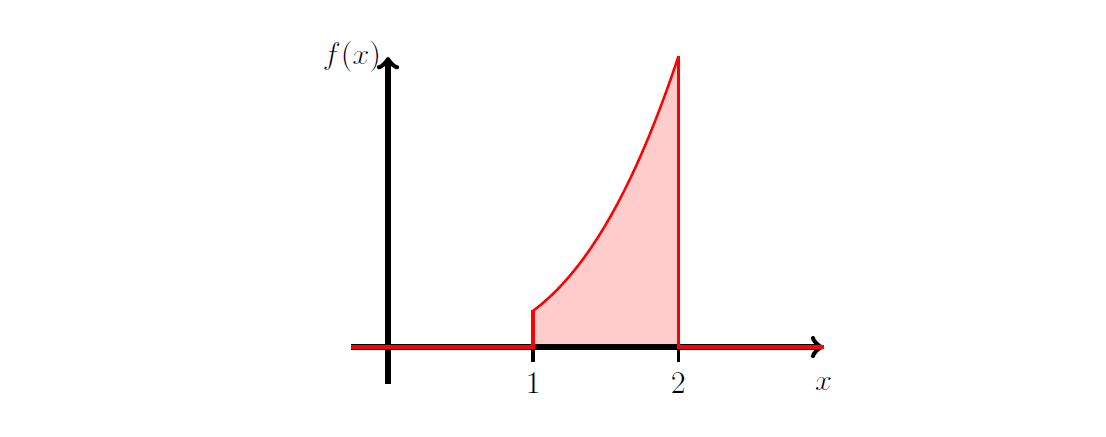
\includegraphics[width=1\linewidth]{Images/density_ex} \caption{Plot of $f_X (x)$.}\label{fig:density1}
\end{figure}

\begin{enumerate}
\def\labelenumi{\arabic{enumi}.}
\tightlist
\item
  Show that \(k =4/15\);\\
\item
  Find \(P (\frac{5}{4}\le X \le \frac{7}{4})\).
\item
  Compute the standard deviation of \(X\).\\
  \emph{Remember:} Standard deviation is the square root of the variance.\\
\item
  Find the median of \(X\).\\
\end{enumerate}

Attempt \protect\hyperlink{rv:exer:cts_example}{Example 5.3.6} and then watch \protect\hyperlink{video10}{Video 10} for the solutions.

Watch \href{https://mediaspace.nottingham.ac.uk/media/Continuous+Distribution+FINAL+VERSION/1_m4k87ypu}{\textcolor{blue}{Video 10: Continuous random variable}}

Solution to Example 5.3.6.

\begin{enumerate}
\def\labelenumi{\arabic{enumi}.}
\tightlist
\item
  Remember \(\int_{-\infty}^\infty f_X (x) \, dx =1\) and therefore\\

  \begin{eqnarray*}
  1 &=& \int_{-\infty}^\infty f_X (x) \, dx \\
  &=& \int_1^2 k x^3 \, dx \\
  &=& k \left[ \frac{x^4}{4} \right]_1^2 \\
  &=& k \left(\frac{2^4}{4} -\frac{1^4}{4} \right)  = k \times \frac{15}{4}.
  \end{eqnarray*}

  Thus, \(k=\frac{4}{15}\).\\
\item
  It follows from the above that the c.d.f of \(X\) is\\

  \[ F_X (x) = \left\{ \begin{array}{ll} 0 & \mbox{for } x<1 \\ \int_1^x \frac{4}{15}y^3 \, dy = \frac{x^4-1}{15} & \mbox{for } 1 \leq x \leq 2 \\  1 & \mbox{for } x>2  \end{array} \right. \]

  Thus

  \begin{eqnarray*}
  P \left(\frac{5}{4}  \leq X \leq \frac{7}{4}\right) &=& \frac{(7/4)^4-1}{15} - \frac{(5/4)^4-1}{15} \\
  &=& \frac{1}{15} \left[\left( \frac{7}{4}\right)^4 -\left( \frac{5}{4}\right)^4 \right] \\
  &=& \frac{37}{80} (=0.4625).
  \end{eqnarray*}
\item
  Remember that the standard deviation of \(X\) is the square root of the variance. Therefore\\

  \[ sd (X) = \sqrt{var(X)} = \sqrt{E[X^2]- E[X]^2}. \]
\end{enumerate}

For any \(n=1,2,\ldots\),\\

\begin{align*} E[X^n] &= \int_{-\infty}^\infty x^n f_X(x) \, dx \\
&= \int_1^2 x^n \frac{4}{15} x^3 \, dx \\
&= \frac{4}{15} \left[\frac{x^{n+4}}{n+4} \right]_1^2 \\
&= \frac{4 (2^{n+4}-1)}{15(n+4)}. \end{align*}

Therefore\\

\begin{align*} 
E [X] &= \frac{4 (32-1)}{15 \times 5} = \frac{124}{75} = 1.6533 \\
E [X^2] &= \frac{4 (64-1)}{15 \times 6} = \frac{14}{5} = 2.8 \end{align*}

Thus\\

\[ sd (X) = \sqrt{2.8 -1.6533^2} = 0.2579. \]

\begin{enumerate}
\def\labelenumi{\arabic{enumi}.}
\setcounter{enumi}{3}
\tightlist
\item
  The median of \(X\), \(m\), satisfies\\

  \begin{eqnarray*}
  0.5 &=& P (X \leq m) = \frac{m^4 -1}{15} \\
  7.5 &=& m^4 -1 \\
  8.5 &=& m^4.
  \end{eqnarray*}
\end{enumerate}

Therefore\\

\[ m = (8.5)^{1/4} =1.7075. \]

\hfill\break

\hypertarget{rv:bernoulli}{%
\section{Bernoulli distribution and its extension}\label{rv:bernoulli}}

In this section, we start with the \protect\hyperlink{rv:Bernoulli:bern}{Bernoulli} random variable, which is the simplest non-trivial probability distribution taking two possible values (0 or 1). In itself the Bernoulli random variable might not seem particularly exciting, but it forms a key building block in probability and statistics. We consider probability distributions which arise as extensions of the Bernoulli random variable such as the \protect\hyperlink{rv:Bernoulli:bin}{Binomial} distribution (sum of \(n\) Bernoulli random variables), the \protect\hyperlink{rv:Bernoulli:geom}{Geometric} distribution (number of Bernoulli random variables until we get a 1) and the \protect\hyperlink{rv:Bernoulli:negbin}{Negative Binomial} distribution (number of Bernoulli random variables until we get our \(n^{th}\) 1).

\hypertarget{rv:Bernoulli:bern}{%
\subsection{Bernoulli distribution}\label{rv:Bernoulli:bern}}

\leavevmode\vadjust pre{\hypertarget{rv:def:Bernoulli}{}}%
\textcolor{red}{Definition 5.4.1.}
{\textbf{Bernoulli trial.}}

A \emph{Bernoulli trial} is a simple random experiment with two outcomes: success \((1)\) or failure \((0)\). The success probability is \(p\), so failure probability = \(1-p (=q)\).
A Bernoulli random variable \(X\) describes this:\\

\begin{eqnarray*}
X =
\left\{
\begin{array}{ll}
1 & \mbox{success - probability $p$}, \\
0 & \mbox{failure - probability $q=1-p$.}
\end{array}
\right.
\end{eqnarray*}

The Bernoulli distribution has probability mass function:\\

\[ p_X (x) = p^x (1-p)^{1-x} \hspace{1cm} x=0,1. \]

{[}If \(x =1\),
\(p_X (1) = p^1 q^0 = p\) and if \(x=0\), \(p_X (0) = p^0 q^1 = q\).{]}

We have that

\[
E[X]= [p \times 1] + [q \times 0] = p
\]

and\\

\[
E[X^{2}] = [p \times 1^{2}] + [q \times 0^{2}] = p.
\]

Therefore\\

\[
var (X) = E[X^{2}] - E[X]^{2} = p - p^{2} = p(1-p) =pq.
\]

\hypertarget{rv:Bernoulli:bin}{%
\subsection{Binomial Distribution}\label{rv:Bernoulli:bin}}

\hypertarget{rv:def:iid}{}
\textcolor{red}{Definition 5.4.2.}
{\textbf{Independent and identically distributed}}\\
Two discrete random variables \(X\) and \(Y\) are said to be \textbf{independent and
identically distributed} (\emph{i.i.d.}) if for all \(x, y \in \mathbb{R}\),\\

\[ P(X=x, Y=y) = P(X=x) \times P(Y=y) \hspace{0.5cm} (\mbox{independence}) \]

and for all \(x \in \mathbb{R}\),\\

\[ P(Y=x) = P(X=x), \]

(identically distributed, \emph{i.e.} have the same pmf.)

\hfill\break

\leavevmode\vadjust pre{\hypertarget{rv:def:bin}{}}%
\textcolor{red}{Definition 5.4.3.}
{\textbf{Binomial distribution.}}

Consider \(n\) independent Bernoulli trials, each with
success probability \(p\). Let \(X\) be the total number of successes. Then \(X\) has
a \emph{Binomial} distribution, written\\

\[
X \sim {\rm Bin}(n,p), \; \; \mbox{or } X \sim {\rm B}(n,p)
\]

and for \(k = 0, 1, \ldots, n\),\\

\[
p_X(k) = P(X = k) = \binom{n}{k} p^{k}(1-p)^{n-k} .
\]

To see this: consider any particular sequence of \(k\) successes and \(n-k\)
failures. Each such sequence has probability \(p^{k}(1-p)^{n-k}\), since the \(n\) trials are independent.
There are \(\binom{n}{k}\) ways of choosing the positions of the \(k\) successes out of \(n\) trials.

\textbf{Note:}
1. \(n\) and \(p\) are called the parameters of the Binomial distribution.\\
2. The number of trials \(n\) is fixed.\\
3. There are only two possible outcomes: `success' with probability \(p\) and `failure' with probability \(q =1-p\).\\
4. The probability of success \(p\) in each independent trial is constant.

\leavevmode\vadjust pre{\hypertarget{rv:lem:binomial_expectation}{}}%
\textcolor{red}{Lemma 5.4.4.}
{\textbf{Binomial distribution: Expectation and variance.}}

Let \(X \sim {\rm Bin} (n,p)\), then\\

\[ E[X]=np \hspace{0.5cm} \mbox{and} \hspace{0.5cm} var(X) = n p(1-p). \]

We can write\\

\begin{equation}   
X = X_1 + X_2 + \ldots + X_n, 
\label{eq:bin1}  
\end{equation}

where \(X_1, X_2, \ldots, X_n\) are independent Bernoulli random variables each with success probability \(p\).

Therefore using properties of expectations\\

\begin{align*}
E [X] & = E [ X_1 + X_2 + \ldots + X_n ] \\
&=  E [ X_1 ]+ E [X_2] + \ldots + E [X_n ]  \\
& = p + p + \ldots + p = np.\end{align*}

Given that the \(X_i\)'s in \eqref{eq:bin1} are independent, we also have that\\

\begin{align*}
var (X) & = var ( X_1 + X_2 + \ldots + X_n ) \\
&= var ( X_1) + var (X_2) + \ldots + var (X_n ) \\
& = p(1-p) + p(1-p) + \ldots + p(1-p) = np(1-p).\end{align*}

\hfill\break

The cumulative distribution function is\\

\[
F_X (x) = P (X \leq x) = \sum_{k=0}^{[x]} \binom{n}{k} p^{k}(1-p)^{n-k},
\]

where \([x]\) is the greatest integer not greater than \(x\).

An \textbf{R Shiny} app is provided to explore the Binomial distribution.

R Shiny app: \href{https://shiny-new.maths.nottingham.ac.uk/pmzpn/Binomial/}{Binomial distribution}

\hypertarget{rv:ex:mc}{}
\textcolor{red}{Example 5.4.5.}\\
Twenty multiple choice questions, each with 5 options. Suppose that you
guess at random, independently for each question. Then if \(X\) is the number of
right answers,\\

\[
X \sim Bin(20,0.2).
\]

Then\\

\[
P(X = 3) = \binom{20}{3} (0.2)^{3}(0.8)^{17} =0.2053,
\]

and\\

\[
P(X \leq 3) = \sum_{k=0}^{3} \binom{20}{k} (0.2)^{k}(0.8)^{20-k} = 0.4114.
\]

\hypertarget{rv:Bernoulli:geom}{%
\subsection{Geometric Distribution}\label{rv:Bernoulli:geom}}

\leavevmode\vadjust pre{\hypertarget{rv:def:geometric}{}}%
\textcolor{red}{Definition 5.4.6.}
{\textbf{Geometric distribution.}}

Consider a sequence of independent Bernoulli trials each with success probability \(p\). Let \(Y\) denote the number of trials needed for the first success to appear. Then \(Y\) has a \emph{Geometric} distribution with parameter \(p\), written \(Y \sim Geom(p)\), and\\

\[
p_Y (k) = (1-p)^{k-1}p, \; \; \; k = 1, 2, 3, \ldots .
\]

\emph{To see this:} If the \(k^{th}\) trial is the first success then the first \(k-1\) trials must have
been failures. Probability of this is \((1-p)^{k-1}p\).

Note that\\

\[
\sum_{k=1}^\infty p_Y (k)=\sum_{k=1}^\infty (1-p)^{k-1}p=p\sum_{i=0}^\infty (1-p)^i=\frac{p}{1-(1-p)}=1,
\]

so a success eventually occurs with probability \(1\).

\leavevmode\vadjust pre{\hypertarget{geometric_expectation}{}}%
\textcolor{red}{Lemma 5.4.7.}
{\textbf{Geometric distribution: Expectation and variance.}}

Let \(Y \sim {\rm Geom} (p)\), then\\

\[ E[Y]= \frac{1}{p} \hspace{0.5cm} \mbox{and} \hspace{0.5cm} var(Y) = \frac{1-p}{p^2}. \]

First step: Let \(q=1-p\) and write

\begin{eqnarray*}
E[Y] & = & \sum_{k=1}^{\infty} k P(Y=k) \\ & = & \sum_{k=1}^{\infty} k (1-p)^{k-1}p \\
 & = & p \sum_{k=1}^{\infty} k q^{k-1} \end{eqnarray*}

Note that \(k q^{k-1}\) is the derivative of \(q^k\) with respect to \(q\). Hence,

\begin{eqnarray*}
E[Y] & = & p \sum_{k=1}^{\infty} \frac{{\rm d} \;}{{\rm d}q} \left\{ q^{k} \right\}.
\end{eqnarray*}

We can interchange the order of summation and differentiation (we won't go into the technical requirements):

\begin{eqnarray*}
E [Y] & = & p \frac{{\rm d} \;}{{\rm d}q} \left( \sum_{k=1}^{\infty} q^k\right) \\
& = & p \frac{{\rm d} \;}{{\rm d}q} \left( \frac{q}{1-q}\right),
 \end{eqnarray*}

since \(\sum_{k=1}^\infty x^k = x/(1-x)\) if \(|x| <1\).

Therefore

\begin{eqnarray*}
E [Y] & = & p \frac{(1)(1-q)- q(-1)}{(1-q)^2}\\
& = & \frac{p}{p^2} = \frac{1}{p}.
 \end{eqnarray*}

By a similar method, we obtain

\[
E[Y(Y-1)] =  \frac{2(1-p)}{p^{2}}.
\]

Since
\begin{equation}
E[Y(Y-1)]= E[Y^2-Y] = E[Y^2] -E[Y], 
\label{eq:sec}
\end{equation}
we have that

\[
var(Y) = E[Y(Y-1)] + E[Y] - E[Y]^{2} = \frac{1-p}{p^{2}}.
\]

\hypertarget{rv:Bernoulli:negbin}{%
\subsection{Negative binomial Distribution}\label{rv:Bernoulli:negbin}}

\leavevmode\vadjust pre{\hypertarget{rv:def:neg_binom}{}}%
\textcolor{red}{Definition 5.4.8.}
{\textbf{Negative binomial distribution.}}

Consider a sequence of independent Bernoulli trials, each with success probability \(p\). If \(W\) is
the number of trials needed until \(r\) successes have occurred then \(W\) has a \emph{Negative
Binomial} distribution, \(W \sim {\rm Neg Bin} (r,p)\), with probability mass function

\[
p_W (k) = \binom{k-1}{r-1}p^{r}(1-p)^{k-r} \; \; \; k = r, r+1, \ldots
\]

\emph{To see this:} We must have the \(k^{th}\) trial is successful and that it is the \(r^{th}\) success. Therefore we have \(r-1\) successes in first \(k-1\) trials, the locations of which can be chosen in \(\binom{k-1}{r-1}\) ways.

\leavevmode\vadjust pre{\hypertarget{rv:lem:neg_binom_expectation}{}}%
\textcolor{red}{Lemma 5.4.9.}
{\textbf{Negative binomial distribution: Expectation and variance.}}

Let \(W \sim {\rm Neg Bin} (r,p)\), then

\[ E[W]= \frac{r}{p} \hspace{0.5cm} \mbox{and} \hspace{0.5cm} var(W) =  \frac{r(1-p)}{p^2}. \]

Note that we can write

\[
W = Y_{1} + Y_{2} + \ldots + Y_{r},
\]

where \(Y_1\) is the number of trials until the first success and, for \(i=2,3,\dots,r\), \(Y_i\) is the number of trials after the \((i-1)^{st}\) success until the \(i^{th}\) success.

We observe that \(Y_1, Y_2,\dots,Y_r\) are independent \({\rm Geom}(p)\) random variables, so

\[
E[Y_1]= \frac{1}{p} \qquad\mbox{and}\qquad var(Y_1)= \frac{1-p}{p^2},
\]

whence

\[
E[W] = E[Y_{1} + Y_{2} +\ldots + Y_{r}] =E[Y_{1}]+E[Y_{2}]+\ldots+E[Y_{r}]  = \frac{r}{p},
\]

and

\[
var(W) = var(Y_{1} + Y_{2} +\ldots +Y_{r}) =var(Y_{1})+var(Y_{2})+\ldots+var(Y_{r}) = \frac{r(1-p)}{p^{2}}.
\]

\hfill\break

The negative binomial distribution \(W \sim {\rm Neg Bin} (r,p)\) is the sum of \(r\) independent geometric, \(Y \sim {\rm Geom} (p)\) distributions in the same way that the binomial distribution \(X \sim {\rm Bin} (n,p)\) is the sum of \(n\) independent Bernoulli random variables with success probability \(p\).

An \textbf{R Shiny} app is provided to explore the Negative Binomial distribution.

R Shiny app: \href{https://shiny-new.maths.nottingham.ac.uk/pmzpn/NegBin/}{Negative Binomial distribution}

\protect\hyperlink{rv:exer:crazy_golf}{Example 5.4.10} draws together the different Bernoulli-based distributions and demonstrates how they are used to answer different questions of interest.

\hypertarget{rv:exer:crazy_golf}{}
\textcolor{red}{Example 5.4.10.}
{\textbf{Crazy golf.}}\\
\strut \\

\begin{figure}
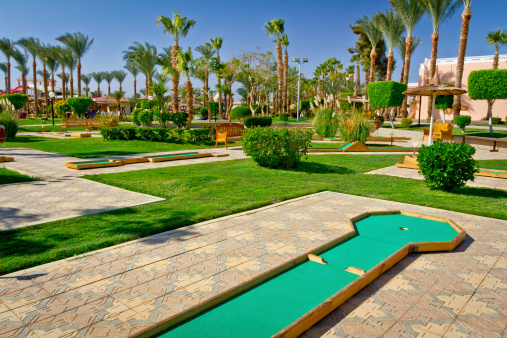
\includegraphics[width=0.8\linewidth]{Images/crazygolf1} \caption{Crazy golf picture.}\label{fig:golf1}
\end{figure}

A child plays a round of crazy golf. The round of golf consists of 9 holes. The number of shots the child takes at each
hole is geometrically distributed with success probability 0.25.

\begin{enumerate}
\def\labelenumi{(\alph{enumi})}
\tightlist
\item
  Calculate the probability that the child gets a `hole in
  one' on the first hole. (A `hole in one' means the child only takes
  one shot on that hole.)\\
\item
  Calculate the probability that the child takes more than five shots on the first hole.\\
\item
  Calculate the probability that the child gets three `hole in one' during their round.
\item
  Calculate the mean and variance for the total number of shots the child takes.\\
\item
  Calculate the probability that the child takes 36 shots in completing their round.\\
\end{enumerate}

Attempt \protect\hyperlink{rv:exer:crazy_golf}{Example 5.4.10 (Crazy golf)} and then watch \protect\hyperlink{video11}{Video 11} for the solutions.

Watch \href{https://mediaspace.nottingham.ac.uk/media/Crazy+Golf+FINAL+VERSION/1_n6lfsnjm}{\textcolor{blue}{Video 11: Crazy Golf Example}}

Solution to Example 5.4.10.

Let \(X_i\) denote the number of shots taken on hole \(i\). Then \(X_i \sim {\rm Geom} (0.25)\).

\begin{enumerate}
\def\labelenumi{(\alph{enumi})}
\tightlist
\item
  A `hole in one' on the first hole is the event \(\{ X_1 =1\}\). Therefore
\end{enumerate}

\[ P(\mbox{Hole in one}) = P(X_1 =1) =0.25. \]

\begin{enumerate}
\def\labelenumi{(\alph{enumi})}
\setcounter{enumi}{1}
\tightlist
\item
  More than five shots on the first hole is the event \(\{X_1 >5\}\). Therefore
\end{enumerate}

\[ P(X_1 >5) =0.75^5 = 0.2373. \]

\begin{enumerate}
\def\labelenumi{(\alph{enumi})}
\setcounter{enumi}{2}
\tightlist
\item
  This is a binomial question since there are \(n=9\) holes and on each hole there is \(p=P(X_1 =1) =0.25\) of obtaining a hole in one. Let \(Y \sim {\rm Bin} (9,0.25)\) denote the number of holes in one in a round, then
\end{enumerate}

\[ P(Y=3) = \binom{9}{3} (0.25)^3 (0.75)^6 =0.2336. \]

\begin{enumerate}
\def\labelenumi{(\alph{enumi})}
\setcounter{enumi}{3}
\tightlist
\item
  The total number of shots taken is
\end{enumerate}

\[Z = X_1 + X_2 + \ldots +X_9 \sim {\rm Neg Bin} (9,0.25). \]

Thus the mean number of shots taken is \(E[Z] = \frac{9}{0.25} = 36\) and the variance of the number of shots is \(var (Z) = \frac{9 (1-0.25)}{0.25^2} =108\).\\
(e) The probability that the child takes exactly 36 (mean number of) shots is

\[ P(Z=36) = \binom{36-1}{9-1} (0.25)^9 (0.75)^{27} = 0.0380. \]

\hypertarget{rv:Poisson}{%
\section{Poisson distribution}\label{rv:Poisson}}

The Poisson distribution is often used to model
`random' events - \emph{e.g.} hits on a website; traffic accidents; customers
joining a queue etc.

Suppose that events occur at rate \(\lambda > 0\) per unit time. Divide the time interval \([0,1)\)
into \(n\) small equal parts of length \(1/n\).

\[
[0,1) = \left[ 0, \frac{1}{n} \right) \cup \left[ \frac{1}{n}, \frac{2}{n} \right) \cup \ldots \cup \left[ \frac{i}{n},\frac{i+1}{n} \right)
\cup \ldots \cup \left[ \frac{n-1}{n},1 \right).
\]

Assume that each interval can have either zero or one event, independently of other intervals, and

\[
P \left[ \mathrm{1~event~in} \left[ \frac{i}{n}, \frac{i+1}{n} \right) \right] = \frac{\lambda}{n}.
\]

\begin{figure}

\includegraphics[width=1\linewidth]{Images/pois1} \caption{Four events (red crosses) in 50 sub-intervals of [0,1].}\label{fig:pois1}
\end{figure}

Let \(X\) be the number of events in the time interval \([0,1)\).
Then

\[ X \sim \mathrm{Bin} (n, \lambda/n) \]

and letting \(n \to \infty\), (the number of intervals grows but the chance of observing an event in a given interval decreases), we have that

\begin{eqnarray*}
P (X=k) & = & \binom{n}{k} \left( \frac{\lambda}{n} \right)^{k} \left( 1 - \frac{\lambda}{n}
\right)^{n-k} \\
& = & \frac{n (n-1) \ldots (n-k+1)}{k!} \times \frac{\lambda^{k}}{n^k} \times \left( 1 - \frac{\lambda}{n}
\right)^{n-k} \\
& = & \frac{n (n-1) \ldots (n-k+1)}{n^k} \times \frac{\lambda^{k}}{k!}\times
\frac{ (1 - \lambda / n)^n}{(1 - \lambda / n )^k}  \\
& = & 1 \left(1 - \frac{1}{n} \right) \cdots \left(1 - \frac{(k-1)}{n} \right) \times \frac{\lambda^k}{k!}
\times \frac{ (1 - \lambda / n)^n}{(1 - \lambda / n )^k}  \\
& \rightarrow & 1 \times  \frac{\lambda^k}{k!} \times \exp(-\lambda)
\; \; \mbox{ as $n \to \infty$, for fixed $k$}.
\end{eqnarray*}

\leavevmode\vadjust pre{\hypertarget{rev:def:Poisson}{}}%
\textcolor{red}{Definition 5.5.1.}
{\textbf{Poisson distribution}}

Let \(X\) be a \textbf{discrete} random variable with parameter \(\lambda >0\) and p.m.f.

\[P(X=x) = \frac{\lambda^x}{x!} \exp(-\lambda) \hspace{1cm} (x=0,1,\ldots).\]

Then \(X\) is said to follow a \textbf{Poisson} distribution with parameter \(\lambda\), denoted \(X \sim {\rm Po} (\lambda)\).

\leavevmode\vadjust pre{\hypertarget{rev:lem:poisson_expectation}{}}%
\textcolor{red}{Lemma 5.5.2.}
{\textbf{Poisson distribution: Expectation and variance.}}

Let \(X \sim {\rm Po} (\lambda)\), then

\[ E[X]= \lambda \hspace{0.5cm} \mbox{and} \hspace{0.5cm} var(X) =  \lambda. \]

By definition of expectation,

\[
E[X] = \sum_{x=0}^\infty x P(X=x) = \sum_{x=1}^\infty x P(X=x), \]

since \(0 \times P(X=0) =0\).

Now

\begin{eqnarray*}
E[X] &=& \sum_{x=1}^\infty x \times \frac{\lambda^x}{x!} \exp(-\lambda) \\
&=& \exp(-\lambda) \sum_{x=1}^\infty \frac{x \lambda^x}{x!} = \lambda \exp(-\lambda) \sum_{x=1}^\infty \frac{ \lambda^{x-1}}{(x-1)!}. \end{eqnarray*}

Using a change of variable \(k=x-1\),

\[ E[X]= \lambda \exp(-\lambda) \sum_{k=0}^\infty \frac{ \lambda^k}{k!} = \lambda \exp(-\lambda) \exp(\lambda) =\lambda. \]

Similarly, we can show that

\[ E[X(X-1)] = \sum_{x=0}^\infty x (x-1) \left( \frac{\lambda^x}{x!} \exp(-\lambda) \right) = \lambda^2.  \]

Therefore, as noted in \protect\hyperlink{geometric_expectation}{Lemma 5.4.7} \eqref{eq:sec}, we have that \(E[X^2]=E[X(X-1)] + E[X]\) giving

\begin{eqnarray*}
var(X) &=& E[X(X-1)] + E[X] - E[X]^2 \\
 &=&  \lambda^2 + \lambda - \lambda^2 = \lambda. 
\end{eqnarray*}

\hypertarget{rv:exponential}{%
\section{Exponential distribution and its extensions}\label{rv:exponential}}

In this section we start with the \protect\hyperlink{rv:exponential:exp}{Exponential} random variable which is an important continuous distribution that can take positive values (on the range \([0,\infty)\)). The Exponential distribution is the continuous analogue of the \protect\hyperlink{rv:Bernoulli:geom}{Geometric} distribution. The sum of exponential distributions leads to the \href{https://en.wikipedia.org/wiki/Erlang_distribution}{Erlang distribution} which is a special case of the \protect\hyperlink{rv:exponential:gamma}{Gamma distribution}. Another special case of the Gamma distribution is the \protect\hyperlink{rv:exponential:chi}{\(\chi^2\) (Chi squared) distribution} which is important in statistics. Finally, we consider the \protect\hyperlink{rv:exponential:beta}{Beta distribution} which is continuous distribution taking values on the range \((0,1)\) and can be constructed from Gamma random variables via a transformation. (See \protect\hyperlink{Transform}{Section 14} for details on transformations.)

\hypertarget{rv:exponential:exp}{%
\subsection{Exponential distribution}\label{rv:exponential:exp}}

Let \(X\) denote the total number of hits on a website in time \(t\).
Let \(\lambda\) - rate of hits per unit time, and so, \(\lambda t\) -
rate of hits per time \(t\).

A suitable model as we have observed in \protect\hyperlink{rv:Poisson}{Section 5.5} for \(X\) is \({\rm Po} (\lambda t)\).

Let \(T\) denote the time, from a fixed point, until the first hit. Note that \(T\) is
continuous \(0 < T < \infty\) whilst the number of hits \(X\) is
discrete. Then \(T > t\) if and only if \(X=0\). Hence,

\[  P(T > t) = P (X=0) = \exp(-\lambda t) \]

and so,

\[ P (T \leq t) = 1 - \exp(-\lambda t) \; \; \; (t > 0). \]

Therefore the cumulative distribution function of T is

\[ F_T (t) = \left\{ \begin{array}{ll} 0 & t < 0 \\ 1 - \exp(-\lambda
t) & t \geq 0 \end{array} \right. \]

Differentiating \(F_T (t)\) with respect to \(t\) gives

\[ f_T (t) = \left\{ \begin{array}{ll} 0 & t < 0 \\ \lambda \exp(- \lambda t) & t \geq 0 \end{array} \right. \]

\leavevmode\vadjust pre{\hypertarget{rv:def:exponential}{}}%
\textcolor{red}{Definition 5.6.1.}
{\textbf{Exponential distribution}}

A random variable \(T\) is said to have an exponential distribution
with parameter \(\lambda > 0\), written \(T \sim {\rm Exp} (\lambda)\) if its
c.d.f. is given by
\[ F_T (t) = \left\{ \begin{array}{ll} 1- e^{- \lambda t} & t>0 \\
0 & t \leq 0, \end{array} \right. \]
and its p.d.f. is
\[ f_T (t) = \frac{d \;}{dt} F_T (t) = \left\{ \begin{array}{ll} \lambda
e^{- \lambda t} & t>0 \\
0 & t \leq 0 \end{array} \right. \]

\leavevmode\vadjust pre{\hypertarget{rv:lem:exponential_expectation}{}}%
\textcolor{red}{Lemma 5.6.2.}
{\textbf{Exponential distribution: Expectation and variance.}}

Let \(T \sim {\rm Exp} (\lambda)\), then
\[ E[T]= \frac{1}{\lambda} \hspace{0.5cm} \mbox{and} \hspace{0.5cm} var(T) = \frac{1}{\lambda^2}. \]

The expectation of \(T\) is

\[ E[T] = \int_{-\infty}^\infty t f_T (t) \, dt = \int_0^\infty t
\lambda e^{- \lambda t} \, dt. \]

Using integration by parts, we have that

\begin{eqnarray*} E[T] &=& \left[ t \times - e^{-\lambda t} \right]_0^\infty -
\int_0^\infty - e^{-\lambda t} \, dt \\
&=& (0-0) + \left[ - \frac{1}{\lambda} e^{-\lambda t}
\right]_0^\infty  = \frac{1}{\lambda}.\end{eqnarray*}

Similarly, by using integration parts twice,

\[ E[T^2] = \int_0^\infty
t^2 \lambda e^{- \lambda t} \, dx = \frac{2}{\lambda^2}. \]

Therefore
the variance of \(T\) is

\[ var (T) = E[T^2] - E[T]^2 = \frac{2}{\lambda^2} -
\frac{1}{\lambda^2} = \frac{1}{\lambda^2}. \]

\hfill\break

\hypertarget{rv:exponential:gamma}{%
\subsection{Gamma distribution}\label{rv:exponential:gamma}}

Suppose that we want to know, \(W\), the time until the \(m^{th}\) \((m=1,2,\ldots)\) hit on a website. Then \[W=T_1 + T_2 + \ldots + T_m \]
where \(T_i\) is the time from the \((i-1)^{st}\) hit on the website until the \(i^{th}\) hit on the website.

\begin{figure}
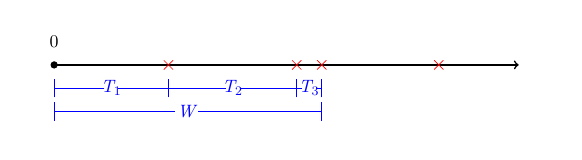
\includegraphics[width=1\linewidth]{Images/Gamma1} \caption{Illustration with $m=3$, $W=T_1 +T_2 +T_3$.}\label{fig:gamma1}
\end{figure}

Note that \(T_1,T_2, \ldots\) are independent and identically distributed \protect\hyperlink{rv:def:iid}{i.i.d.} according to \(T \sim {\rm Exp} (\lambda)\). That is, \(W\) is the sum of \(m\) exponential random variables with parameter \(\lambda\). Then \(W\) follows a Gamma distribution with \(W \sim {\rm Gamma} (m,\lambda)\).

\leavevmode\vadjust pre{\hypertarget{rv:def:gamma_rv}{}}%
\textcolor{red}{Definition 5.6.3.}
{\textbf{Gamma distribution}}

A random variable \(X\) is said to have a Gamma distribution with
parameters \(\alpha, \beta > 0\), written \(X \sim {\rm Gamma} (\alpha, \beta)\)
if its p.d.f. is given by

\[ f_X (x) = \left\{ \begin{array}{ll} \frac{\beta^\alpha}{\Gamma (\alpha)}
x^{\alpha -1} \exp(- \beta x) & x>0 \\
0 & x \leq 0, \end{array} \right. \]

where \(\Gamma (\alpha) = \int_0^\infty y^{\alpha -1} \exp(-y) \, dy\).

Note that if \(\alpha\) is an integer \(\Gamma (\alpha) = (\alpha -1)!\). Also \(\Gamma \left( \frac{1}{2} \right) = \sqrt{\pi}\) and for
\(\alpha > 1\),

\[ \Gamma (\alpha) = (\alpha -1) \Gamma (\alpha -1). \]

By definition, for \(\alpha =1\), \(X \sim {\rm Exp} (\beta)\) and for \(\alpha \in \mathbb{N}\), the Gamma distribution is given by the sum of \(\alpha\) exponential random variables. The special case where \(\alpha\) is integer is sometimes referred to as the \textbf{Erlang distribution}. However, the gamma distribution is defined for positive, real-valued \(\alpha\).

The \(\alpha\) parameter is known as the \emph{shape} parameter and determines the shape of the Gamma distribution. In particular, the shape varies dependent on whether \(\alpha <1\), \(\alpha =1\) or \(\alpha >1\).

\begin{itemize}
\tightlist
\item
  \(\alpha <1\), the modal value of \(X\) is at 0 and \(f(x) \to \infty\) as \(x \downarrow 0\) (\(x\) tends to 0 from above).\\
\item
  \(\alpha =1\), the exponential distribution. The modal value of of \(X\) is at 0 and \(f(0)=\beta\).\\
\item
  \(\alpha >1\), \(f(0)=0\) and the modal value of \(X\) is at \(\frac{\alpha-1}{\beta}\).
\end{itemize}

The \(\beta\) parameter is known as the \emph{scale} parameter. It does not affect the shape of the Gamma distribution but has the property that if \(U \sim {\rm Gamma} (\alpha,1)\), then \(X\) has the same distribution as \(U/\beta\). This can be written as

\[ X \stackrel{D}{=} \frac{U}{\beta} \sim \frac{1}{\beta} {\rm Gamma} (\alpha,1). \]

\leavevmode\vadjust pre{\hypertarget{rv:def:eqd}{}}%
\textcolor{red}{Definition 5.6.4.}
{\textbf{Equality in distribution}}

Two random variables \(X\) and \(Y\) are said to be \emph{equal in distribution}, denoted \(X \stackrel{D}{=} Y\), if for all \(x \in \mathbb{R}\),

\[ P(X \leq x) = P(Y \leq x). \]

That is, \(X\) and \(Y\) have the same c.d.f., or equivalently, \(X\) and \(Y\) have the same p.d.f. (p.m.f.) if \(X\) and \(Y\) are continuous (discrete).

An \textbf{R Shiny} app is provided to explore the Gamma distribution.

R Shiny app: \href{https://shiny-new.maths.nottingham.ac.uk/pmzpn/Gamma/}{Gamma distribution}

\leavevmode\vadjust pre{\hypertarget{rv:lem:gamma_expectation}{}}%
\textcolor{red}{Lemma 5.6.5.}
{\textbf{Gamma distribution: Expectation and variance.}}

If \(X \sim {\rm Gamma} (\alpha, \beta)\) then

\[
E[X] = \frac{\alpha}{\beta}, \; \; \; var(X) = \frac{\alpha}{\beta^{2}}.
\]

The proof is straightforward if \(\alpha =m \in \mathbb{N}\) since then \(X= T_1 +T_2 + \ldots +T_m\), where the \(T_i\) are \emph{i.i.d.} according to \(T \sim {\rm Exp} (\beta)\). (Compare with the proof of \protect\hyperlink{rv:lem:neg_binom_expectation}{Lemma 5.4.9} for the mean and variance of the negative binomial distribution.)

We omit the general proof for \(\alpha \in \mathbb{R}^+\), which can be proved by integration by parts.

We have noted that the Gamma distribution arises as the sum of exponential distributions. More general if \(X_1 \sim {\rm Gamma} (\alpha_1, \beta)\) and \(X_2 \sim {\rm Gamma} (\alpha_2, \beta)\) are independent gamma random variables with a common scale parameter \(\beta >0\), then

\[
X_1 + X_2 \sim {\rm Gamma} (\alpha_1 + \alpha_2, \beta).
\]

\hypertarget{rv:exponential:chi}{%
\subsection{Chi squared distribution}\label{rv:exponential:chi}}

The chi squared (\(\chi^2\)) distribution is a special case of the Gamma distribution which plays an important role in statistics. For \(k \in \mathbb{N}\), if

\[ X \sim {\rm Gamma} \left(\frac{k}{2}, \frac{1}{2} \right) \]

then \(X\) is said to follow a chi squared distribution with \(k\) degrees of freedom. Note that \(X\) has probability density function

\[ f_X (x) = \left\{ \begin{array}{ll} \frac{x^{\frac{k}{2}-1} \exp\left(-\frac{x}{2}\right)}{2^{\frac{k}{2}} \Gamma \left( \frac{k}{2}\right)} & x>0 \\
0 & x \leq 0, \end{array} \right. \]

with \(E[X] =k\) and \(var(X) =2k\).

\hypertarget{rv:exponential:beta}{%
\subsection{Beta distribution}\label{rv:exponential:beta}}

Suppose that \(X\) and \(Y\) are \textbf{independent} random variables such that \(X \sim {\rm Gamma} (\alpha, \gamma)\) and \(Y \sim {\rm Gamma} (\beta, \gamma)\) for some \(\alpha, \beta, \gamma >0\). Note that both \(X\) and \(Y\) have the same scale parameter \(\gamma\). Let

\[ Z = \frac{X}{X+Y},\]

the proportion of the sum of \(X\) and \(Y\) accounted for by \(X\). Then \(Z\) will take values on the range \([0,1]\) and \(Z\) follows a Beta distribution with parameters \(\alpha\) and \(\beta\).

\leavevmode\vadjust pre{\hypertarget{rv:def:beta}{}}%
\textcolor{red}{Lemma 5.6.6.}
{\textbf{Beta distribution}}

A random variable \(Z\) is said to have a Beta distribution with
parameters \(\alpha, \beta > 0\), written \(Z \sim {\rm Beta} (\alpha, \beta)\) if its pdf is given by

\[ f_Z (z) = \left\{ \begin{array}{ll} \frac{\Gamma (\alpha + \beta)}{
\Gamma (\alpha) \Gamma (\beta)} z^{\alpha -1} (1- z)^{\beta -1} & 0 < z < 1 \\
0 & \mbox{otherwise.} \end{array} \right. \]

Note that if \(Z \sim {\rm Beta} (\alpha, \beta)\), then

\[ E[Z] = \frac{\alpha}{\alpha+\beta} \hspace{.5cm} \mbox{and} \hspace{.5cm} var (Z) = \frac{\alpha \beta}{(\alpha + \beta)^2 (\alpha + \beta +1)}.  \]

The special case where \(\alpha = \beta =1\), \(f_Z (z)=1\) \((0<z<1)\) and \(Z\) is uniformly distributed on \([0,1]\) denoted \(Z \sim U(0,1)\). That is,

\[ {\rm Beta} (1,1) \stackrel{D}{=} U(0,1). \]

An \textbf{R Shiny} app is provided to explore the Beta distribution.

R Shiny app: \href{https://shiny-new.maths.nottingham.ac.uk/pmzpn/Beta/}{Beta distribution}

\protect\hyperlink{rv:exer:catch_bus}{Example 5.6.7 (Catching a bus)} draws together the different Exponential-based distributions and demonstrates how they are used to answer different questions of interest.

\leavevmode\vadjust pre{\hypertarget{rv:exer:catch_bus}{}}%
\textcolor{red}{Example 5.6.7.}
{\textbf{Catching a bus.}}

\begin{figure}

\includegraphics[width=0.8\linewidth]{Images/bus} \caption{Bus picture.}\label{fig:bus}
\end{figure}

Suppose that the time (in minutes) between buses arriving at a bus stop follows an Exponential distribution, \(Y \sim {\rm Exp} (0.5)\). Given you arrive at the bus stop just as one bus departs:

\begin{enumerate}
\def\labelenumi{(\alph{enumi})}
\tightlist
\item
  Calculate the probability that you have to wait more than 2
  minutes for the bus.\\
\item
  Calculate the probability that you have to wait more than 5
  minutes for the bus given that you wait more than 3 minutes.\\
\item
  Given that the next two buses are full, what is the probability you have to wait more than 6 minutes for a bus (the third bus to arrive)?\\
\item
  What is the probability that the time until the third bus arrives is more than double the time until the second bus arrives?\\
\end{enumerate}

Attempt \protect\hyperlink{rv:exer:catch_bus}{Example 5.6.7 (Catching a bus)} and then watch \protect\hyperlink{video12}{Video 12} for the solutions.

Watch \href{https://mediaspace.nottingham.ac.uk/media/Catch+The+Bus+FINAL+VERSION/1_vtwjyiai}{\textcolor{blue}{Video 12: Catching a bus}}

Solution to Example 5.6.7.

For an exponential random variable, \(X \sim {\rm Exp} (\beta)\), we have that for any \(x>0\),

\[ P(X >x) = 1 - P(X \leq x) = 1- \{ 1 -\exp(-\beta x) \} = \exp(-\beta x).\]

\begin{enumerate}
\def\labelenumi{(\alph{enumi})}
\tightlist
\item
  Since \(Y \sim {\rm Exp} (0.5)\),

  \[ P(Y >2) = \exp (-0.5(2)) = \exp(-1) =0.3679.\]
\item
  Note that \(\{Y>5\}\) implies that \(\{Y > 3\}\). Therefore

  \[ P(Y>5|Y>3) = \frac{P(Y >5)}{P(Y>3)} = \frac{\exp(-0.5(5))}{\exp(-0.5(3))} = \exp(-1) =0.3679.\]

  Therefore

  \[ P(Y > 5 |Y >3) = P(Y>2). \]

  This property is known as the \textbf{memoryless} property of the exponential distribution, for any \(s,t>0\),

  \[ P(Y > s+t| Y>s) = P(Y >t).\]
\item
  The time, \(W\), until the third bus arrives is \(W \sim {\rm Gamma} (3,0.5)\). Therefore

  \[ f_W (w) = \frac{0.5^3}{(3-1)!} w^{3-1} \exp(-0.5 w)  \hspace{1cm} (w>0), \]

  and

  \[ F_W (w) = 1- \exp (-0.5 w) \left[ 1 + 0.5 w + \frac{(0.5w)^2}{2} \right]. \]
\end{enumerate}

Hence,\\

\[P(W>6) = 1 -F_W(6) = \exp(-0.5(6)) \left[ 1 +0.5(6) + \frac{(0.5\times 6)^2}{2} \right] = 0.4232.\]

\begin{enumerate}
\def\labelenumi{(\alph{enumi})}
\setcounter{enumi}{3}
\tightlist
\item
  This question involves the beta distribution. Let \(Z\) denote the time until the second bus arrives and let \(T\) denote the time between the second and third bus arriving. Then we want \[P(Z+T>2Z). \]
  Rearranging \(Z+T >2 Z\), we have that this is equivalent to

  \[\frac{1}{2}> \frac{Z}{Z+T},\]

  where

  \[\frac{Z}{Z+T} = U \sim {\rm Beta} (2,1)\]

  with \(U\) having p.d.f.

  \[ f_U (u) = \frac{(2+1-1)!}{(2-1)! (1-1)!} u^{2-1} (1-u)^{1-1} = 2u \hspace{1cm} (0<u<1).\]

  Hence

  \begin{eqnarray*} P(Z+T>2Z) &=&P(U < 0.5)  \\ &=& \int_0^{0.5} 2 u \, du \\ &=& \left[ u^2 \right]_0^{0.5} =0.25. 
  \end{eqnarray*}
\end{enumerate}

\hypertarget{rv:normal}{%
\section{Normal (Gaussian) Distribution}\label{rv:normal}}

\leavevmode\vadjust pre{\hypertarget{rv:def:normal}{}}%
\textcolor{red}{Definition 5.7.1.}
{\textbf{Normal (Gaussian) distribution.}}

\(X\) is said to have a normal distribution, \(X \sim N(\mu, \sigma^{2})\), if it has p.d.f.

\[
f_X (x) = \frac{1}{\sqrt{2 \pi} \, \sigma} \exp \left( - \frac{1}{2 \sigma^2} [x-\mu]^2 \right), \quad \quad  x \in \mathbb{R},
\]

where \(\mu \in \mathbb{R}\) and \(\sigma > 0\).

The parameters \(\mu\) and \(\sigma\) of the normal distribution specify the mean and standard deviation with

\[ E[X] = \int_{- \infty}^{\infty} x f_X(x) \; dx = \mu\]

and

\[ E[X^2] =  \int_{- \infty}^{\infty} x^{2} f_X(x) \; dx = \sigma^{2} + \mu^{2}\]

giving

\[ var (X) = E[X^2] - E[X]^2 = \sigma^2.\]

The normal distribution is symmetric about its mean \(\mu\) with the p.d.f. decreasing as \([x-\mu]^2\) increases. Therefore the median and mode of the normal distribution are also equal to \(\mu\). See Figure \ref{fig:normalpdf} for the p.d.f. and c.d.f. of \(N(0,1)\).

\leavevmode\vadjust pre{\hypertarget{rv:def:normal_cdf}{}}%
\textcolor{red}{Definition 5.7.2.}\\
The c.d.f. of the normal distribution \(X \sim N(\mu,\sigma^2)\) is
\[ F_X(x) = \int_{-\infty}^x f(y) \;dy = \int_{-\infty}^x \frac{1}{\sqrt{2 \pi} \sigma} \exp \left( - \frac{1}{2 \sigma^2} [y-\mu]^2 \right) \;dy, \]
and has no analytical solution. (\emph{i.e.} We cannot solve the integral.)

How do we proceed with the Normal distribution if we cannot compute its c.d.f.?

The simplest solution is to use a statistical package such as \textbf{R} to compute probabilities (c.d.f.) for the Normal distribution. This can be done using the \texttt{pnorm} function. However, it is helpful to gain an understanding of the Normal distribution and how to compute probabilities (c.d.f.) for the Normal distribution using the good old-fashioned method of Normal distribution tables.

The starting point is to define the \emph{standard normal distribution}, \(Z \sim N(0,1)\). We can then show that for any \(X \sim N(\mu,\sigma^2)\) and \(a, b \in \mathbb{R}\), \(P(a < X<b)\) can be rewritten as
\[ P(a <X <b) = P(c <Z<d) = P(Z<d) - P(Z<c)\]
where \(c\) and \(d\) are functions of \((a,\mu,\sigma)\) and \((b,\mu,\sigma)\), respectively. It is thus sufficient to know the c.d.f. of \(Z\). Note that when \(Z\) is used to define a normal distribution it will always be reserved for the standard normal distribution.

Traditionally, probabilities for \(Z\) are obtained from \emph{Normal tables}, tabulated values of \(P(Z<z)\) for various values of \(z\). Typically, \(P(Z <z)\) for \(z=0.00,0.01,\ldots,3.99\) are reported with the observation \[P(Z <-z) = 1-P(Z<z)\] used to obtain probabilities for negative values.

A normal table will usually look similar to the table below.

\begin{longtable}[]{@{}
  >{\raggedright\arraybackslash}p{(\columnwidth - 12\tabcolsep) * \real{0.0896}}
  >{\raggedright\arraybackslash}p{(\columnwidth - 12\tabcolsep) * \real{0.1493}}
  >{\raggedright\arraybackslash}p{(\columnwidth - 12\tabcolsep) * \real{0.1493}}
  >{\raggedright\arraybackslash}p{(\columnwidth - 12\tabcolsep) * \real{0.1493}}
  >{\raggedright\arraybackslash}p{(\columnwidth - 12\tabcolsep) * \real{0.1493}}
  >{\raggedright\arraybackslash}p{(\columnwidth - 12\tabcolsep) * \real{0.1493}}
  >{\raggedright\arraybackslash}p{(\columnwidth - 12\tabcolsep) * \real{0.1642}}@{}}
\toprule\noalign{}
\begin{minipage}[b]{\linewidth}\raggedright
z
\end{minipage} & \begin{minipage}[b]{\linewidth}\raggedright
0
\end{minipage} & \begin{minipage}[b]{\linewidth}\raggedright
1
\end{minipage} & \begin{minipage}[b]{\linewidth}\raggedright
2
\end{minipage} & \begin{minipage}[b]{\linewidth}\raggedright
3
\end{minipage} & \begin{minipage}[b]{\linewidth}\raggedright
4
\end{minipage} & \begin{minipage}[b]{\linewidth}\raggedright
\(\cdots\)
\end{minipage} \\
\midrule\noalign{}
\endhead
\bottomrule\noalign{}
\endlastfoot
0.0 & 0.5 & 0.504 & 0.508 & 0.512 & 0.516 & \(\cdots\) \\
0.1 & 0.5398 & 0.5438 & 0.5478 & 0.5517 & 0.5557 & \(\cdots\) \\
\(\vdots\) & \(\vdots\) & \(\vdots\) & \(\vdots\) & \(\vdots\) & \(\vdots\) & \(\ddots\) \\
1.2 & 0.8849 & 0.8869 & 0.8888 & 0.8907 & 0.8925 & \(\cdots\) \\
\(\vdots\) & \(\vdots\) & \(\vdots\) & \(\vdots\) & \(\vdots\) & \(\vdots\) & \(\ddots\) \\
\end{longtable}

The first column, labelled \(z\), increments in units of \(0.1\). Columns 2 to 11 are headed 0 through to 9. To find \(P(Z <z) = P(Z<r.st)\) where \(z=r.st\) and \(r,s,t\) are integers between 0 and 9, inclusive, we look down the \(z\) column to the row \(r.s\) and then look along the row to the column headed \(t\). The entry in row ``\(r.s\)'' and column ``\(t\)'' is \(P(Z<r.st)\). For example, \(P(Z <1.22) = 0.8888\).

\leavevmode\vadjust pre{\hypertarget{standard_normal}{}}%
\textcolor{red}{Definition 5.7.3.}
{\textbf{Standard Normal distribution.}}

If \(\mu = 0\) and \(\sigma = 1\) then \(Z \sim N(0,1)\) has a \emph{standard normal} distribution with p.d.f.
\[
\phi(x) = \frac{1}{\sqrt{2 \pi}} \, {\rm e}^{-x^{2}/2 }, \; \; \; x \in \mathbb{R},
\]
and c.d.f.
\[
\Phi (x)  = \int_{- \infty}^{x} \frac{1}{\sqrt{2 \pi}} \, {\rm e}^{-y^{2}/2 } \; dy
\]
Note the notation \(\phi (\cdot)\) and \(\Phi (\cdot)\) which are commonly used for the p.d.f. and c.d.f. of \(Z\).

\begin{figure}
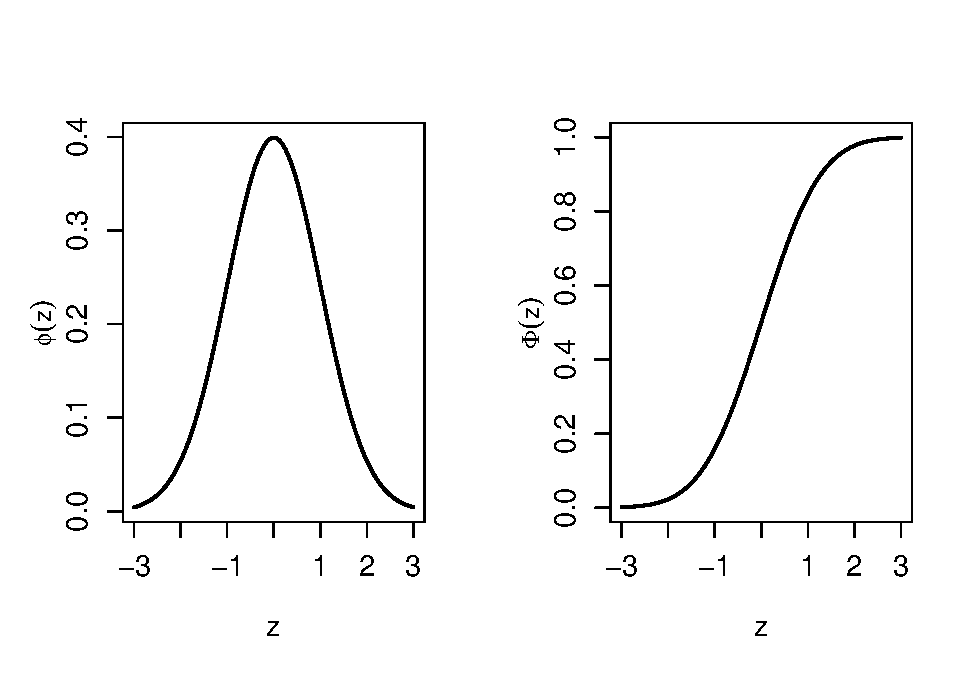
\includegraphics[width=0.7\linewidth]{_main_files/figure-latex/normalpdf-1} \caption{Standard normal, Z~N(0,1), p.d.f. and c.d.f.}\label{fig:normalpdf}
\end{figure}

\leavevmode\vadjust pre{\hypertarget{rv:lem:tranform_normal}{}}%
\textcolor{red}{Lemma 5.7.4.}
{\textbf{Transformation of a Normal random variable.}}

If \(X \sim N(\mu, \sigma^2)\) and \(Y=aX+b\) then
\[ Y \sim N (a \mu +b, a^2 \sigma^2).\]

An immediate Corollary of \protect\hyperlink{rv:lem:tranform_normal}{Lemma 5.7.4} is that if \(X \sim N(\mu, \sigma^2)\), then
\[ \frac{X - \mu}{\sigma} = Z \sim N(0,1).\]
This corresponds to setting \(a=1/\sigma\) and \(b=-\mu/\sigma\) in \protect\hyperlink{rv:lem:tranform_normal}{Lemma 5.7.4}.

Hence, for any \(x \in \mathbb{R}\),

\[ P (X \leq x) = P \left( \frac{X-\mu}{\sigma} \leq \frac{x-\mu}{\sigma} \right) = P \left( Z \leq \frac{x-\mu}{\sigma} \right) = \Phi \left( \frac{x-\mu}{\sigma} \right).\]

\leavevmode\vadjust pre{\hypertarget{rv:def:normal_quantile}{}}%
\textcolor{red}{Definition 5.7.5.}
{\textbf{Percentage points}}

The inverse problem of finding for a given \(q\) \((0<q<1)\), the value of \(z\) such that \(P(Z < z)=q\) is often tabulated for important choices of \(q\). The function \texttt{qnorm} in \textbf{R} performs this function for general \(X \sim N(\mu,\sigma^2)\).

\leavevmode\vadjust pre{\hypertarget{rv:def:normal_sums}{}}%
\textcolor{red}{Definition 5.7.6.}
{\textbf{Sums of Normal random variables}}

Suppose that \(X_1, X_2, \ldots, X_n\) are \emph{independent} normal random variables with \(X_i \sim N(\mu_i, \sigma_i^2)\). Then for \(a_1, a_2, \ldots, a_n \in \mathbb{R}\),

\[ Y = \sum_{i=1}^n a_i X_i \sim N \left( \sum_{i=1}^n a_i \mu_i, \sum_{i=1}^n a_i^2 \sigma_i^2 \right).\]

\hfill\break

\leavevmode\vadjust pre{\hypertarget{rv:exer:lemonade}{}}%
\textcolor{red}{Example 5.7.7.}
{\textbf{Lemonade dispenser}}

Suppose that the amount of lemonade dispensed by a machine into a cup is
normally distributed with mean \(250 \, ml\) and standard deviation \(5\, ml\). Suppose that the cups used for the lemonade are normally
distributed with mean \(260 \, ml\) and standard deviation \(4 \, ml\).

\begin{enumerate}
\def\labelenumi{(\alph{enumi})}
\tightlist
\item
  What is the probability that the lemonade overflows the cup?\\
\item
  What is the probability that the total lemonade in 8 cups exceeds \(1970 ml\)?\\
\end{enumerate}

Attempt \protect\hyperlink{rv:exer:lemonade}{Example 5.7.7 (Lemonade dispenser)} and then watch \protect\hyperlink{video13}{Video 13} for the solutions.

Watch \href{https://mediaspace.nottingham.ac.uk/media/Lemonade+Example+FINAL+VERSION/1_prbx0h86}{\textcolor{blue}{Video 13: Lemonade dispenser}}

Solution to Example 5.7.7

\begin{enumerate}
\def\labelenumi{(\alph{enumi})}
\tightlist
\item
  Let \(L\) and \(C\) denote the amount of lemonade dispensed and the size of a cup (in \(ml\)), respectively. Then \(L \sim N(250,5^2)\) and \(C \sim N(260,4^2)\), and we want:

  \[ P(C <L) = P(C-L <0).\]

  Note that \(C-L\) follows a normal distribution (use \protect\hyperlink{rv:def:normal_sums}{Definition 5.7.6. Sums of Normal random variables} with \(n=2\), \(X_1 =C\), \(X_2=L\), \(a_1 =1\) and \(a_2 =-1\)) with \(C-L \sim N(260-250,25+16) = N(10,41)\).
\end{enumerate}

Therefore, if \(Y \sim N(10,41)\),

\[ P(C<L) = P(Y <0) = P \left( \frac{Y-10}{\sqrt{41}} < \frac{0-10}{\sqrt{41}} \right) = \Phi \left(-1.56 \right) = 0.0594.\]

Note that the answer is given by \texttt{pnorm(-1.56)} and for the answer rounded to 4 decimal places \texttt{round(pnorm(-1.56),4)}.

\begin{enumerate}
\def\labelenumi{(\alph{enumi})}
\setcounter{enumi}{1}
\tightlist
\item
  Let \(L_i \sim N(250,5^2)\) denote the total number of lemonade dispensed into the \(i^{th}\) cup. Then the total amount of lemonade dispensed into 8 cups is \(S = L_1 + L_2 + \ldots + L_8 \sim N (2000,200)\). Therefore

  \[ P(S >1970) = P \left( \frac{S -2000}{\sqrt{200}} >\frac{1970 -2000}{\sqrt{200}} \right) = P(Z>-2.12) = 1 - \Phi (-2.12) = 0.9830. \]
\end{enumerate}

\hfill\break

\hypertarget{prob:lab}{%
\section*{\texorpdfstring{{\textbf{Student Exercises}}}{Student Exercises}}\label{prob:lab}}
\addcontentsline{toc}{section}{{\textbf{Student Exercises}}}

Attempt the exercises below.

\leavevmode\vadjust pre{\hypertarget{exer5:1}{}}%
\textcolor{red}{Exercise 5.1.}\\
Let \(X\) be a continuous random variable with pdf
\[ f_X(x)= \left\{ \begin{array}{ll} k x^3 & \text{if } 0<x<1, \\
k e^{1-x} & \text{if } x \ge 1, \\
0 & \text{otherwise.} \end{array} \right.\]

\begin{enumerate}
\def\labelenumi{(\alph{enumi})}
\tightlist
\item
  Evaluate \(k\) and find the (cumulative) distribution function of \(X\).\\
\item
  Calculate \(P (0.5<X<2)\) and \(P(X>2|X>1)\).
\end{enumerate}

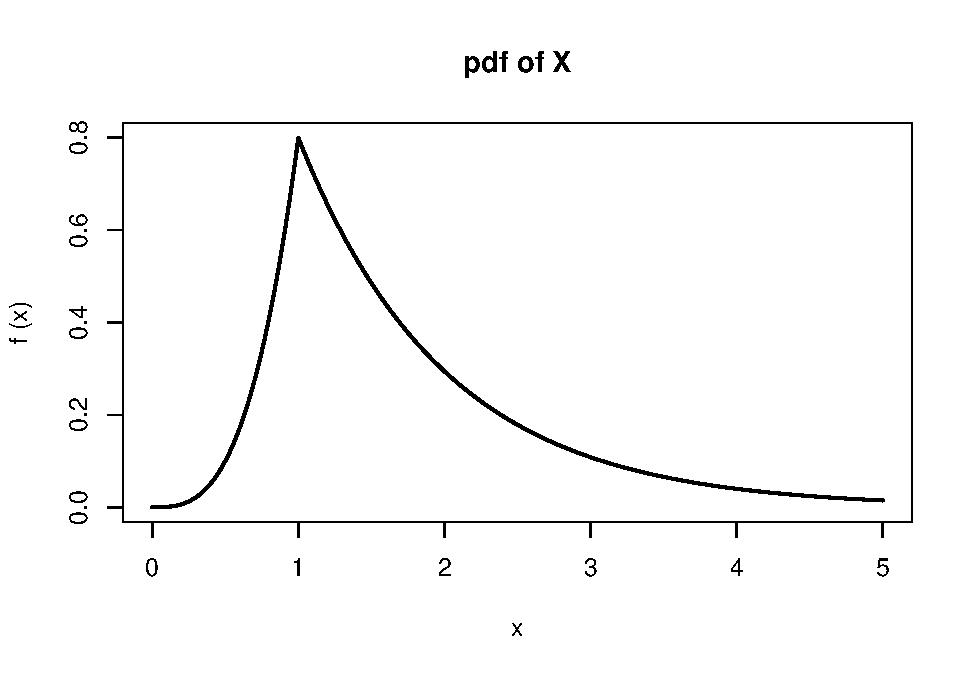
\includegraphics{_main_files/figure-latex/unnamed-chunk-113-1.pdf} 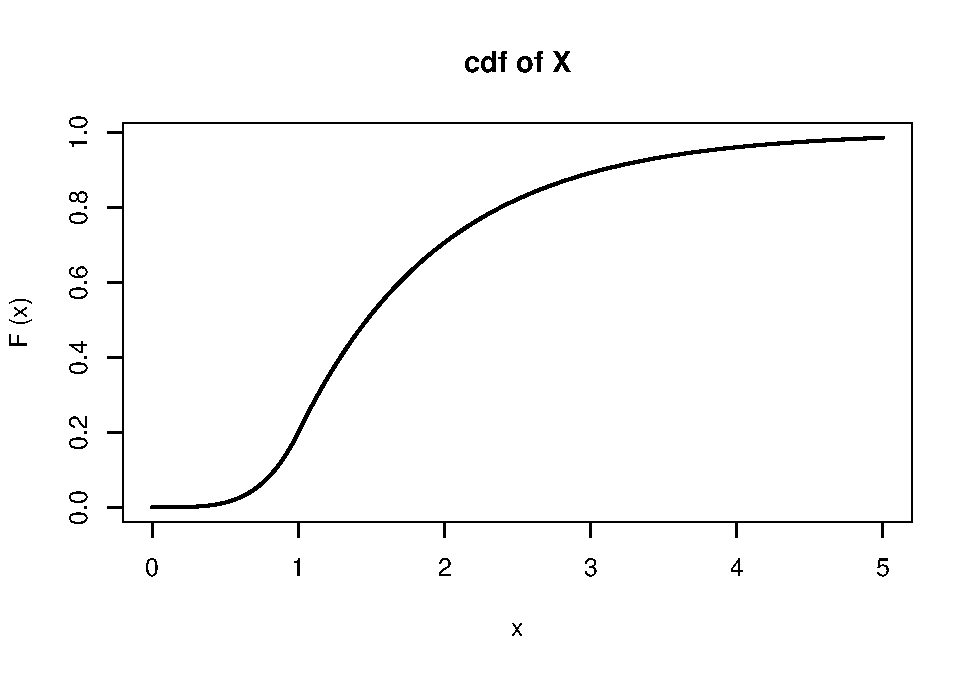
\includegraphics{_main_files/figure-latex/unnamed-chunk-113-2.pdf}

\hfill\break

\leavevmode\vadjust pre{\hypertarget{exer5:2}{}}%
\textcolor{red}{Exercise 5.2.}\\
The time that a butterfly lives after emerging from its chrysalis is a random variable \(T\), and the probability that it survives for more than \(t\) days is equal to \(36/(6+t)^2\) for all \(t>0\).

\begin{enumerate}
\def\labelenumi{(\alph{enumi})}
\tightlist
\item
  What is the probability that it will die within six days of emerging?\\
\item
  What is the probability that it will live for between seven and fourteen days?\\
\item
  If it has lived for seven days, what is the probability that it will live at least seven more days?\\
\item
  If a large number of butterflies emerge on the same day, after how many days would you expect only \(5\%\) to be alive?\\
\item
  Find the pdf of \(T\).\\
\item
  Calculate the mean life of a butterfly after emerging from its chrysalis.\\
\end{enumerate}

\hfill\break

\leavevmode\vadjust pre{\hypertarget{exer5:3}{}}%
\textcolor{red}{Exercise 5.3.}\\
A type of chocolate bar contains, with probability \(0.1\), a prize voucher.
Whether or not a bar contains a voucher is independent of other bars. A hungry
student buys 8 chocolate bars. Let \(X\) denote the number of vouchers that she finds.

\begin{enumerate}
\def\labelenumi{(\alph{enumi})}
\tightlist
\item
  What sort of distribution does \(X\) have?\\
\item
  How likely is it that the student finds no vouchers?\\
\item
  How likely is it that she finds at least two vouchers?\\
\item
  What is the most likely number of vouchers that she finds?
\end{enumerate}

A second student keeps buying chocolate bars until he finds a voucher. Let \(Y\)
denote the number of bars he buys.

\begin{enumerate}
\def\labelenumi{(\alph{enumi})}
\setcounter{enumi}{4}
\tightlist
\item
  What is the probability mass function of \(Y\)?\\
\item
  How likely is it that the student buys more than 5 bars?\\
\item
  What is \(E[Y]\)?
\item
  If each bar costs 35p, what is the expected cost to the student?
\end{enumerate}

A third student keeps buying chocolate bars until they find 4 vouchers. In
doing so, they buys a total of \(W\) bars.

\begin{enumerate}
\def\labelenumi{(\roman{enumi})}
\tightlist
\item
  What is the distribution of \(W\)?\\
\end{enumerate}

\begin{enumerate}
\def\labelenumi{(\alph{enumi})}
\setcounter{enumi}{9}
\tightlist
\item
  What is the probability that this student buys exactly 10 bars?\\
\end{enumerate}

\hfill\break

\leavevmode\vadjust pre{\hypertarget{exer5:4}{}}%
\textcolor{red}{Exercise 5.4.}\\
A factory produces nuts and bolts on two independent machines. The external diameter of the bolts is normally distributed with mean 0.5 cm and the internal diameter of the nuts is normally distributed with mean 0.52 cm. The two machines have the same variance which is determined by the rate of production. The nuts and bolts are produced at rate which corresponds to a standard deviation \(\sigma=0.01\) cm and a third machine fits each nut on to the corresponding bolt as they are produced, provided the diameter of the nut is strictly greater than that of the bolt, otherwise it rejects both.

\begin{enumerate}
\def\labelenumi{(\alph{enumi})}
\tightlist
\item
  Find the probability that a typical pair of nut and bolt is rejected.\\
\item
  If successive pairs of nut and bolt are produced independently, find the probability that in 20 pairs of nut and bolt at least 1 pair is rejected.\\
\item
  The management wishes to reduce the probability that a typical pair of nut and bolt is rejected to 0.01. What is the largest value of \(\sigma\) to achieve this?
\end{enumerate}

\hfill\break

\hypertarget{jointdis}{%
\chapter{Joint Distribution Functions}\label{jointdis}}

\hypertarget{jointdis:intro}{%
\section{Overview}\label{jointdis:intro}}

In \protect\hyperlink{rv}{Section 5} we have introduced the concept of a random variable and a variety of discrete and continuous random variables. However, often in statistics it is important to consider the joint
behaviour of two (or more) random variables. For example:

\begin{enumerate}
\def\labelenumi{(\roman{enumi})}
\tightlist
\item
  Height, Weight.\\
\item
  Degree class, graduate salary.
\end{enumerate}

In this section we explore the joint distribution between two random variables \(X\) and \(Y\).

\hypertarget{jointdis:cdf}{%
\section{Joint c.d.f. and p.d.f.}\label{jointdis:cdf}}

\leavevmode\vadjust pre{\hypertarget{jointdis:def:cdf}{}}%
\textcolor{red}{Definition 6.2.1.}
{\textbf{Joint c.d.f.}}

The \emph{joint (cumulative) probability distribution function} (joint c.d.f.) of \(X\) and \(Y\) is defined by

\begin{align*}
F_{X,Y}(x,y) &= P( \{ \omega: X(\omega) \leq x \text{ and } Y(\omega) \leq y \} )\\
&= P (X \leq x, Y \leq y),
\end{align*}

where \(x,y \in \mathbb{R}\).

\leavevmode\vadjust pre{\hypertarget{jointdis:def:pdf}{}}%
\textcolor{red}{Definition 6.2.2.}
{\textbf{Joint p.d.f.}}

Two r.v.'s \(X\) and \(Y\) are said to be \emph{jointly continuous}, if there exists a function \(f_{X,Y}(x,y) \geq 0\) such that for every ``nice'' set \(C \subseteq {\mathbb R}^2\),

\[P( (X,Y) \in C) = \int\int_C f_{X,Y}(x,y) \,dx \,dy.\]

The function \(f_{X,Y}\) is called the \emph{joint probability density function} (joint p.d.f.) of \(X\) and \(Y\).

If \(X\) and \(Y\) are jointly continuous, then

\begin{align*}
F_{X,Y}(x,y) &= P(X \leq x, Y \leq y) \\
&= \int_{-\infty}^y \int_{-\infty}^x f_{X,Y}(u,v) \,du \,dv.
\end{align*}

Hence we differentiate the c.d.f. \(F_{X,Y}(x,y)\) with respect to both \(x\) and \(y\) to obtain the p.d.f.

\[f_{X,Y}(x,y) = \frac{ \partial^2 \; \; \;\;} {\partial x \partial y} F_{X,Y}(x,y).\]

We note, as in the following example, that often the joint p.d.f. is non-zero on a subset of \(\mathbb{R}^2\).

\hypertarget{jointdis:ex:joint_density_function_ex}{}
\textcolor{red}{Example 6.2.3.}\\
Suppose that

\[f_{X,Y}(x,y) = \begin{cases}
24x(1-x-y) \quad \text{if } x,y \geq 0 \text{ and } x+y \leq 1, \\
0 \qquad \qquad \qquad \quad \text{otherwise.}
\end{cases}\]

\begin{enumerate}
\def\labelenumi{(\alph{enumi})}
\tightlist
\item
  Find \(P(X>Y)\),\\
\item
  Find \(P(X>\frac{1}{2})\).\\
\end{enumerate}

\hypertarget{jointdis:ex:joint_density_function_sol}{}
\begin{enumerate}
\def\labelenumi{(\alph{enumi})}
\tightlist
\item
  Let \(C = \{ (x,y): x>y \}\) and write \(A=\{ (x,y):f_{X,Y}(x,y)>0\}\). Then,
\end{enumerate}

\[ C \cap A = \{ (x,y); x>0, y>0, x+y<1, x>y \}.\]

\hfill\break

Therefore

\begin{align*}
P(X>Y) &= P((X,Y) \in C) \\
&= \int\int_C f_{X,Y}(x,y) \,dx \,dy \\
&= \int\int_{C \cap A} 24x(1-x-y) \,dx \,dy \\
&= \int_0^{1/2} \int_y^{1-y} 24x(1-x-y) \,dx \,dy \\
&= \int_0^{1/2} \left[ 12x^2 - 8x^3 - 12yx^2 \right]_y^{1-y} \,dy \\
&= \int_0^{1/2} \left( 4 - 12y + 16y^3 \right) dy \\
&= \left[ 4y - 6y^2 + 4y^4 \right]_0^{1/2} \\
&= 2 - \frac{3}{2} + \frac{1}{4} = \frac{3}{4}.
\end{align*}

\begin{enumerate}
\def\labelenumi{(\alph{enumi})}
\setcounter{enumi}{1}
\tightlist
\item
  Let \(D = \{ (x,y): x>1/2 \}\), then
\end{enumerate}

\[ D \cap A = \{ (x,y); x>1/2, y>0, x+y<1 \}.\]

Therefore

\begin{align*}
P(X>1/2) &= P((X,Y) \in D) \\
&= \int\int_D f_{X,Y}(x,y) \,dx \,dy \\
&= \int\int_{D \cap A} 24x(1-x-y) \,dx \,dy \\
&= \int_{1/2}^1 \int_0^{1-x} 24x(1-x-y) \,dy \,dx \\
&= \int_{1/2}^1 \left[ 24xy \left( 1 - x - \frac{1}{2}y \right) \right]_0^{1-x} \,dx \\
&= \int_{1/2}^1 12x(1-x)^2 \,dx \\
&= \left[ \frac{12}{2}x^2 - \frac{24}{3}x^3 + \frac{12}{4}x^4 \right]_{1/2}^1 \\
&= 6 - 8 +3 - \frac{3}{2} + 1 - \frac{3}{16} = \frac{5}{16}.
\end{align*}

\hfill\break

\hypertarget{jointdis:marginal}{%
\section{Marginal c.d.f. and p.d.f.}\label{jointdis:marginal}}

There are many situations with bivariate distributions where we are interested in one of the random variables. For example, we might have the joint distribution of height and weight of individuals but only be interested in the weight of individuals. This is known as the \protect\hyperlink{jointdis:def:marginal}{\textbf{marginal distribution}}.

\leavevmode\vadjust pre{\hypertarget{jointdis:def:marginal}{}}%
\textcolor{red}{Definition 6.3.1.}
{\textbf{Marginal c.d.f.}}

Suppose that the c.d.f. of \(X\) and \(Y\) is given by \(F_{X,Y}\), then the c.d.f. of \(X\) can be obtained from \(F_{X,Y}\) since
\begin{align*}
F_X(x) &= P(X \leq x) \\
&=P( X \leq x, Y<\infty ) \\
&= \lim_{y\rightarrow\infty} F_{X,Y}(x,y).
\end{align*}
\(F_X\) is called the \emph{marginal distribution} (marginal c.d.f.) of \(X\).

\leavevmode\vadjust pre{\hypertarget{jointdis:def:marginal:pdf}{}}%
\textcolor{red}{Definition 6.3.2.}
{\textbf{Marginal p.d.f.}}

If \(f_{X,Y}\) is the joint p.d.f. of \(X\) and \(Y\), then the \emph{marginal probability density function} (marginal p.d.f.) of \(X\) is given by
\[f_X(x) = \int_{-\infty}^\infty f_{X,Y}(x,y) \,dy.\]

\leavevmode\vadjust pre{\hypertarget{jointdis:ex:marginal_distributions_ex}{}}%
\textcolor{red}{Example 6.3.3}\\
Consider \protect\hyperlink{jointdis:ex:joint_density_function_ex}{Example 6.2.3}.

Find the marginal p.d.f. and c.d.f of Y.

\hypertarget{jointdis:ex:marginal_distributions_sol}{}
\begin{align*}
f_Y(y) &= \int_{-\infty}^\infty f_{X,Y}(x,y) \,dx \\[9pt]
&= \begin{cases} \int_0^{1-y} 24x(1-x-y) \,dx \quad &0 \leq y \leq 1, \\[5pt]
0 \quad &\text{otherwise.} \end{cases} \\[9pt]
&= \begin{cases} 4(1-y)^3 \quad & 0 \leq y \leq 1, \\[5pt]
0 \quad  &\text{otherwise.} \end{cases}
\end{align*}

Note that marginal distribution of \(Y\) is a \({\rm Beta} (1,4)\) distribution.

Hence,

\begin{align*}
F_Y(y) &= \begin{cases} 0, \quad &y < 0,\\[5pt]
\int_0^y4 (1-u)^3 du = 1-(1-y)^4, \quad &0 \leq y \leq 1,\\[5pt]
1, \quad &y > 1.\end{cases}
\end{align*}

\hfill\break

\hypertarget{jointdis:exer:joint_Z_Exp}{}
\textcolor{red}{Example 6.3.4.}\\
Find the p.d.f. of \(Z=X/Y\), where

\[f_{X,Y}(x,y) =\begin{cases} e^{-(x+y)} \quad &0<x,y<\infty, \\[5pt]
0 \qquad \qquad &\text{otherwise.} \end{cases} \]

Attempt \protect\hyperlink{jointdis:exer:joint_Z_Exp}{Example 6.3.4} and then watch \protect\hyperlink{video14}{Video 14} for the solutions.

Watch \href{https://mediaspace.nottingham.ac.uk/media/Ratio+of+Exponentials+FINAL+VERSION/1_iuf9blt3}{\textcolor{blue}{Video 14: Ratio of Exponentials}}

Solution to Example 6.3.4.

Clearly, \(Z>0\). For \(z>0\),

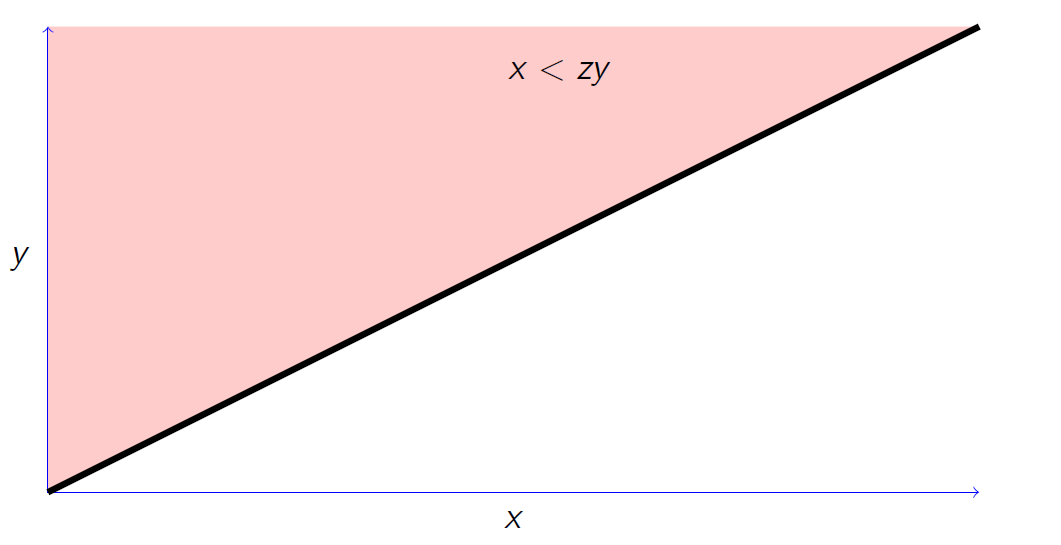
\includegraphics[width=0.7\linewidth]{Images/ratio_exp}

Therefore

\begin{align*}
F_Z(z) &= P( Z \leq z) = P(X/Y \leq z)\\
&= \int\int_{\{(x,y):x/y \leq z\}} f_{X,Y}(x,y) \,dx \,dy \\
&= \int_0^\infty \int_0^{yz} e^{-(x+y)} \,dx\,dy \\
&= \int_0^\infty -e^{-y(1+z)} + e^{-y} \,dy \\
&= 1-\frac{1}{1+z}
\end{align*}

and so

\[ f_Z(z) = \frac{dF_Z(z)}{dz} =\begin{cases} \frac{1}{(1+z)^2}, \quad &z>0, \\
0, \quad  &z \leq 0. \end{cases} \]

\hfill\break

Note that we can extend the notion of joint and marginal distributions to random variables \(X_1,X_2,\dots,X_n\) in a similar fashion.

\hypertarget{jointdis:independent}{%
\section{Independent random variables}\label{jointdis:independent}}

\leavevmode\vadjust pre{\hypertarget{jointdis:def:independent}{}}%
\textcolor{red}{Definition 6.4.1.}
{\textbf{Independent random variables}}

Random variables \(X\) and \(Y\) are said to be \emph{independent} if, for all \(x,y \in \mathbb{R}\),

\[ P(X \leq x, Y \leq y) = P(X \leq x) P(Y \leq y),\]

that is, for all \(x,y\in\mathbb R\), \(F_{X,Y}(x,y) = F_X(x) F_Y(y)\).

If \(X\) and \(Y\) are discrete random variables with joint p.m.f. \(p_{X,Y}(x,y)\) and marginal p.m.f.'s \(p_X(x)\) and \(p_Y(y)\), respectively, then \(X\) and \(Y\) are independent if and only if for all \(x,y\in\mathbb R\),

\[ p_{X,Y}(x,y) = p_X(x)p_Y(y).\]

If \(X\) and \(Y\) are continuous random variables with joint p.d.f. \(f_{X,Y}(x,y)\) and marginal p.d.f.'s \(f_X(x)\) and \(f_Y(y)\), respectively, then \(X\) and \(Y\) are independent if and only if for all \(x,y\in\mathbb R\),

\[ f_{X,Y}(x,y) = f_X(x)f_Y(y).\]

For example, in \protect\hyperlink{jointdis:exer:joint_Z_Exp}{Example 6.3.4} \(X\) and \(Y\) have joint probability density function:

\begin{eqnarray*} f_{X,Y} (x,y) &=& \exp(-\{ x + y\}) \\ &=& \exp (-x) \exp(-y) = f_X (x) f_Y(y), \hspace{0.4cm}(x,y>0),
\end{eqnarray*}

where both \(X\) and \(Y\) are distributed according to \({\rm Exp} (1)\). Thus the distribution \(Z\) given in \protect\hyperlink{jointdis:exer:joint_Z_Exp}{Example 6.3.4} is the ratio of two independent exponential random variables with mean 1.

Note that we can easily extend the notion of independent random variables to random variables \(X_1,X_2,\dots,X_n\).

\leavevmode\vadjust pre{\hypertarget{jointdis:def:iid2}{}}%
\textcolor{red}{Definition 6.4.2.}
{\textbf{Independent and identically distributed}}

The random variables \(X_1,X_2,\dots,X_n\) are said to \emph{independent and identically distributed} (i.i.d.) if,

\begin{itemize}
\item
  \(X_1,X_2,\dots,X_n\) are independent.
\item
  \(X_1,X_2,\dots,X_n\) all have the same distribution, that is, \(X_i \sim F\) for all \(i=1,\dots,n\).
\end{itemize}

\protect\hyperlink{jointdis:def:iid2}{Definition 6.4.2} extends the notion of \emph{i.i.d.} given at the start of \protect\hyperlink{rv:Bernoulli:bin}{Section 5.4.2} for discrete random variables.

\leavevmode\vadjust pre{\hypertarget{jointdis:def:sample}{}}%
\textcolor{red}{Definition 6.4.3.}
{\textbf{Random sample}}

The random variables \(X_1,X_2,\dots,X_n\) are said to be a \emph{random sample} if they are i.i.d.

\textcolor{red}{Definition 6.4.4.}\\
Suppose \(X_1,X_2,\dots,X_n\) are a random sample from the Poisson distribution with mean \(\lambda\). Find the joint p.m.f. of \(X_1,X_2,\dots,X_n\).

\hfill\break

If \(X_i \sim {\rm Po} (\lambda)\), then its p.m.f. is given by

\[ P(X_i = x_i) = p_{X_i}(x_i) = \begin{cases}
\frac{e^{-\lambda} \lambda^{x_i}}{x_i!} \quad &\text{if $x_i=0,1,2,\dots$}, \\
0 \qquad \quad &\text{otherwise.} \end{cases}\]

Since \(X_1,X_2,\dots,X_n\) are independent, their joint p.m.f. is given by,

\begin{align*}
p_{X_1,X_2,\dots,X_n}(x_1,x_2,\dots,x_n) &= \prod_{i=1}^n p_{X_i}(x_i) \\
&= \begin{cases}
\prod_{i=1}^n \frac{ e^{-\lambda} \lambda^{x_i} } {x_i!} \quad &\text{if $x_i=0,1,2,\dots$,} \\
0 \qquad \qquad \quad &\text{otherwise.} \end{cases} \\
&= \begin{cases}
\frac{ e^{-n\lambda} \lambda^{\sum_{i=1}^n x_i} }{\prod_{i=1}^n x_i!} \quad &\text{if $x_i=0,1,2,\dots$,} \\
0 \qquad \qquad \quad &\text{otherwise.} \end{cases}
\end{align*}

\hfill\break

The joint p.m.f. of \(\mathbf{X} = (X_1,X_2, \ldots, X_n)\) tells us how likely we are to observe \(\mathbf{x}= (x_1,x_2,\ldots, x_n)\) given \(\lambda\). This can be used either:

\begin{enumerate}
\def\labelenumi{\arabic{enumi}.}
\tightlist
\item
  To compute \(P (\mathbf{X} = \mathbf{x})\) when \(\lambda\) is known;\\
\item
  Or, more commonly in statistics, to assess what is a \emph{good estimate} of \(\lambda\) given \(\mathbf{x}\) in situations where \(\lambda\) is unknown, see \protect\hyperlink{paraestimate}{Parameter Estimation} in Section 9.
\end{enumerate}

\hypertarget{jointdis:exer}{%
\section*{\texorpdfstring{{\textbf{Student Exercise}}}{Student Exercise}}\label{jointdis:exer}}
\addcontentsline{toc}{section}{{\textbf{Student Exercise}}}

Attempt the exercise below.

\hypertarget{exer6:1}{}
\textcolor{red}{Exercise 6.1.}\\
A theory of chemical reactions suggests that the variation in the quantities \(X\) and \(Y\) of two products \(C_1\) and \(C_2\) of a certain reaction is described by the joint probability density function

\[ f_{X,Y} (x,y) = \frac{2}{(1+x+y)^3} \hspace{1cm} x \geq 0, \; y \geq 0. \]

On the basis of this theory, answer the following questions.

\begin{enumerate}
\def\labelenumi{(\alph{enumi})}
\tightlist
\item
  What is the probability that at least one unit of each product is produced?\\
\item
  Determine the probability that the quantity of \(C_1\) produced is less than half that of \(C_2\).\\
\item
  Find the c.d.f. for the total quantity of \(C_1\) and \(C_2\).\\
\end{enumerate}

\hypertarget{Sec_CLT}{%
\chapter{Central Limit Theorem and law of large numbers}\label{Sec_CLT}}

\hypertarget{Sec_CLT:intro}{%
\section{Introduction}\label{Sec_CLT:intro}}

In this Section we will show why the Normal distribution, introduced in \protect\hyperlink{rv:normal}{Section 5.7}, is so important in probability and statistics. The central limit theorem states that under very weak conditions (almost all probability distributions you will see will satisfy them) the sum of \(n\) \emph{i.i.d.} random variables, \(S_n\), will converge, appropriately \emph{normalised} to a standard Normal distribution as \(n \to \infty\). For finite, but large \(n (\geq 50)\), we can approximate \(S_n\) by a normal distribution and the normal distribution approximation can be used to answer questions concerning \(S_n\). In \protect\hyperlink{Sec_CLT:statement}{Section 7.2} we present the \protect\hyperlink{Sec_CLT:thm:CLT}{\textbf{Central Limit Theorem}} and apply it to an example using exponential random variables. In \protect\hyperlink{Sec_CLT:discrete}{Section 7.3} we explore how a continuous distribution (the Normal distribution) can be used to approximate sums of discrete distributions. Finally, in \protect\hyperlink{Sec_CLT:LLN}{Section 7.4}, we present the \protect\hyperlink{Sec_CLT:thm:LLN}{\textbf{Law of Large Numbers}} which states that the uncertainty in the sample mean of \(n\) observations, \(S_n/n\), decreases as \(n\) increases and converges to the population mean \(\mu\). Both the Central Limit Theorem and the Law of Large Numbers will be important moving forward when considering statistical questions.

\hypertarget{Sec_CLT:statement}{%
\section{Statement of Central Limit Theorem}\label{Sec_CLT:statement}}

Before stating the \protect\hyperlink{Sec_CLT:thm:CLT}{\textbf{Central Limit Theorem}}, we introduce some notation.

\leavevmode\vadjust pre{\hypertarget{Sec_CLT:thm:convd}{}}%
\textcolor{red}{Definition 7.2.1.}
{\textbf{Convergence in distribution}}

A sequence of random variables \(Y_1, Y_2, \ldots\) are said to \textbf{converge in distribution} to a random variable \(Y\), if for all \(y \in \mathbb{R}\),

\[ P(Y_n \leq y) \rightarrow P(Y \leq y) \qquad \qquad \mbox{ as } \; n \to \infty. \]

We write \(Y_n \xrightarrow{\quad D \quad} Y\) as \(n \to \infty\).

\hypertarget{Sec_CLT:thm:CLT}{}
\textcolor{red}{Theorem 7.2.2.}
{\textbf{Central Limit Theorem.}}\\
Let \(X_1,X_2,\dots,X_n\) be independent and identically distributed random variables (i.e.~a random sample) with finite mean \(\mu\) and variance \(\sigma^2\). Let \(S_n = X_1 + \cdots + X_n\). Then

\[ \frac{S_n - n\mu}{\sigma \sqrt{n}} \xrightarrow{\quad D \quad} N(0,1).\]

The central limit theorem is equivalent to

\[\frac{\bar{X} - \mu}{\sigma/\sqrt{n}} \xrightarrow{\quad D \quad} N(0,1).\]

where \(\bar{X} = \frac{1}{n} \sum_{i=1}^n X_i\) is the mean of the distributions \(X_1, X_2, \ldots , X_n\).

Therefore, we have that for large \(n\),

\[ S_n \approx N(n \mu, n \sigma^2) \]

and

\[ \bar{X} \approx N\left(\mu, \frac{\sigma^2}{n} \right). \]

\leavevmode\vadjust pre{\hypertarget{Sec_CLT:ex:clt_exponential}{}}%
\textcolor{red}{Example 7.2.3.}
Suppose \(X_1,X_2,\dots,X_{100}\) are i.i.d. exponential random variables with parameter \(\lambda=4\).

\begin{enumerate}
\def\labelenumi{(\alph{enumi})}
\tightlist
\item
  Find \(P(S_{100} > 30)\).\\
\item
  Find limits within which \(\bar{X}\) will lie with probability \(0.95\).\\
\end{enumerate}

\begin{enumerate}
\def\labelenumi{(\alph{enumi})}
\item
  Since \(X_1,X_2,\dots,X_{100}\) are i.i.d. exponential random variables with parameter \(\lambda=4\), \(E\left[X_i\right]=\frac{1}{4}\) and \(var(X_i) = \frac{1}{16}\). Hence,\\

  \begin{align*}
  E \left[ S_{100} \right] &= 100 \cdot \frac{1}{4} = 25; \\
  var(S_{100}) &= 100 \cdot \frac{1}{16} = \frac{25}{4}.
  \end{align*}

  Since \(n=100\) is sufficiently big, \(S_{100}\) is approximately normally distributed by the central limit theorem (CLT). Therefore,

  \begin{align*}
  P(S_{100} > 30) &= P \left( \frac{S_{100}-25}{\sqrt{\frac{25}{4}}} > \frac{30-25}{\sqrt{\frac{25}{4}}} \right) \\
  &\approx P( N(0,1) >2) \\
  &= 1 - P( N(0,1) \leq 2) \\
  &= 0.0228.
  \end{align*}

  Given that \(S_{100} = \sum_{i=1}^{100} X_i \sim {\rm Gamma} (100,4)\), see \protect\hyperlink{rv:exponential:gamma}{Section 5.6.2}, we can compute exactly \(P(S_{100} >30) = 0.0279\), which shows that the central limit theorem gives a reasonable approximation.
\item
  Since \(X_1,X_2,\dots,X_{100}\) are i.i.d. exponential random variables with parameter \(\lambda=4\), \(E\left[X_i\right]=\frac{1}{4}\) and \(var (X_i) = \frac{1}{16}\). Therefore, \(E\left[\bar{X}\right] = \frac{1}{4}\) and \(var(\bar{X}) = \frac{1/16}{100}\).
\end{enumerate}

Since \(n=100\), \(\bar{X}\) will be approximately normally distributed by the CLT, hence

\begin{align*}
0.95 &= P(a < \bar{X} < b) \\
&= P \left( \frac{a-1/4}{\sqrt{1/1600}} < \frac{\bar{X}-1/4}{\sqrt{1/1600}} < \frac{b-1/4}{\sqrt{1/1600}} \right) \\
&\approx P \left( \frac{a-1/4}{\sqrt{1/1600}} < N(0,1) < \frac{b-1/4}{\sqrt{1/1600}} \right). \\
\end{align*}

There are infinitely many choices for \(a\) and \(b\) but a natural choice is \(P(\bar{X}<a) = P (\bar{X}>b) = 0.025\). That is, we choose \(a\) and \(b\) such that there is equal chance that \(\bar{X}\) is less than \(a\) or greater than \(b\). Thus if for \(0 < q< 1\), \(z_q\) satisfies \(P(Z < z_q)=q\), we have that\\

\begin{align*}
\frac{a-1/4}{\sqrt{1/1600}} &= z_{0.025} = -1.96, \\
\frac{b-1/4}{\sqrt{1/1600}} &= z_{0.975} = 1.96.
\end{align*}

Hence,\\

\begin{align*}
a &= 0.25 - 1.96 \frac{1}{40} = 0.201, \\
b &= 0.25 + 1.96 \frac{1}{40} = 0.299.
\end{align*}

\hfill\break

\hypertarget{Sec_CLT:discrete}{%
\section{Central limit theorem for discrete random variables}\label{Sec_CLT:discrete}}

The central limit theorem can be applied to sums of discrete random variables as well as continuous random variables. Let \(X_1, X_2, \ldots\) be \emph{i.i.d.} copies of a discrete random variable \(X\) with \(E[X] =\mu\) and \(var(X) = \sigma^2\). Further suppose that the support of \(X\) is in the non-negative integers \(\{0,1, \ldots \}\). (This covers all the discrete distributions, we have seen, binomial, negative binomial, Poisson and discrete uniform.)

Let \(Y_n \sim N(n \mu, n \sigma^2)\). Then the central limit theorem states that for large \(n\), \(S_n \approx Y_n\). However, there will exist \(x \in \{0,1,\ldots \}\) such that\\

\[ P(S_n =x) >0 \qquad \qquad \mbox{but} \qquad \qquad P(Y_n =x) =0. \]

The solution is that we approximate\\

\[ P(S_n =x) \qquad \qquad \mbox{by} \qquad \qquad P(x - 0.5 <Y_n \leq x+0.5) =0. \]

This is known as the \textbf{continuity correction}.

\leavevmode\vadjust pre{\hypertarget{Sec_CLT:ex:clt_bernoulli}{}}%
\textcolor{red}{Example 7.3.1.}
Suppose that \(X\) is a Bernoulli random variable with \(P(X=1)=0.6 (=p)\), so \(E[X]=0.6\) and \(var(X) =0.6 \times (1-0.6) =0.24\). Then \[S_n = \sum_{i=1}^n X_i \sim {\rm Bin} (n, 0.6). \]

For \(n=100\), \(S_{100} \sim {\rm Bin} (100, 0.6)\) can be approximated by \(Y\sim N(60,24) (=N(np,np(1-p)))\), see Figure \ref{fig:cltbern}.

\begin{figure}
\includegraphics[width=0.8\linewidth]{_main_files/figure-latex/cltbern-1} \caption{Central limit theorem approximation for the binomial.}\label{fig:cltbern}
\end{figure}

We can see the approximation in Figure \ref{fig:cltbern} in close-up for \(x=54\) to \(56\) in Figure \ref{fig:cltbern55}. The areas marked out by the red lines (normal approximation) are approximately equal to the areas of the bars in the histogram (binomial probabilities).

\begin{figure}
\includegraphics[width=0.8\linewidth]{_main_files/figure-latex/cltbern55-1} \caption{Central limit theorem approximation for the binomial for x=54 to 56.}\label{fig:cltbern55}
\end{figure}

\hypertarget{Sec_CLT:LLN}{%
\section{Law of Large Numbers}\label{Sec_CLT:LLN}}

We observed that
\[ \bar{X} \approx N\left(\mu, \frac{\sigma^2}{n} \right), \]
and the variance is decreasing as \(n\) increases.

Given that \[var (S_n) = var \left(\sum_{i=1}^n X_i \right) = \sum_{i=1}^n var \left( X_i \right) = n \sigma^2,\] we have in general that \[var (\bar{X}) = var \left(\frac{S_n}{n} \right) = \frac{1}{n^2} var (S_n) = \frac{\sigma^2}{n}.\]

A random variable \(Y\) which has \(E[Y]=\mu\) and \(var(Y)=0\) is the \emph{constant}, \(Y \equiv \mu\), that is, \(P(Y=\mu) =1\). This suggests that as \(n \to \infty\), \(\bar{X}\) converges in some sense to \(\mu\). We can make this convergence rigorous.

\leavevmode\vadjust pre{\hypertarget{Sec_CLT:def:convp}{}}%
\textcolor{red}{Definition 7.4.1.}
{\textbf{Convergence in probability}}

A sequence of random variables \(Y_1, Y_2, \ldots\) are said to \textbf{converge in probability} to a random variable \(Y\), if for any \(\epsilon >0\),
\[ P(|Y_n - Y|> \epsilon) \to 0 \qquad \qquad \mbox{ as } \; n \to \infty. \] We write \(Y_n \xrightarrow{\quad p \quad} Y\) as \(n \to \infty\).

We will often be interested in convergence in probability where \(Y\) is a constant.

A useful result for proving convergence in probability to a constant \(\mu\) is Chebychev's inequality. Chebychev's inequality is a special case of the Markov inequality which is helpful in bounding probabilities in terms of expectations.

\leavevmode\vadjust pre{\hypertarget{Sec_CLT:thm:Cheby}{}}%
\textcolor{red}{Theorem 7.4.2.}
{\textbf{Chebychev's inequality.}}\\
Let \(X\) be a random variable with \(E[X] =\mu\) and \(var(X)=\sigma^2\). Then for any \(\epsilon >0\),
\[ P(|X - \mu| > \epsilon) \leq \frac{\sigma^2}{\epsilon^2}. \]

\leavevmode\vadjust pre{\hypertarget{Sec_CLT:thm:LLN}{}}%
\textcolor{red}{Theorem 7.4.3.}
{\textbf{Law of Large Numbers.}}\\
Let \(X_1, X_2, \ldots\) be \emph{i.i.d.} according to a random variable \(X\) with \(E[X] = \mu\) and \(var(X) =\sigma^2\). Then
\[\bar{X} = \frac{1}{n} \sum_{i=1}^n X_i \xrightarrow{\quad p \quad} \mu \qquad \qquad \mbox{ as } \; n \to \infty. \]

First, note that

\[E[\bar{X}] = E \left[ \frac{1}{n} \sum_{i=1}^n X_i \right]= \frac{1}{n} \sum_{i=1}^n E \left[ X_i \right] = \frac{1}{n} (n \mu) = \mu.\]

For any \(\epsilon >0\), we have by \protect\hyperlink{Sec_CLT:thm:Cheby}{Chebychev's inequality} that\\

\[ P(|\bar{X}- \mu| > \epsilon) \leq \frac{1}{\epsilon^2} var (\bar{X}) = \frac{\sigma^2}{n \epsilon^2} \to 0 \qquad \qquad \mbox{ as } n \to \infty, \]

and the Theorem follows.

\leavevmode\vadjust pre{\hypertarget{Sec_clt:exer:clt_dice}{}}%
\textcolor{red}{Example 7.4.4.}
{\textbf{Central limit theorem for dice}}

\begin{figure}
\includegraphics[width=0.8\linewidth]{Images/dice1} \caption{Dice picture.}\label{fig:dice1}
\end{figure}

Let \(D_1, D_2, \ldots\) denote the outcomes of successive rolls of a fair six-sided dice.

Let \(S_n = \sum_{i=1}^n D_i\) denote the total score from \(n\) rolls of the dice and let \(M_n = \frac{1}{n} S_n\) denote the mean score from \(n\) rolls of the dice.

\begin{enumerate}
\def\labelenumi{(\alph{enumi})}
\tightlist
\item
  What is the approximate distribution of \(S_{100}\)?\\
\item
  What is the approximate probability that \(S_{100}\) lies between \(330\) and \(380\), inclusive?\\
\item
  How large does \(n\) need to be such that \(P(|M_n - E[D]|>0.1) \leq 0.01\)?\\
\end{enumerate}

Attempt \protect\hyperlink{Sec_clt:exer:clt_dice}{Example 7.4.4} and then watch \protect\hyperlink{video15}{Video 15} for the solutions.

Watch \href{https://mediaspace.nottingham.ac.uk/media/Dice+CLT+FINAL+VERSION/1_f2v50ix1}{\textcolor{blue}{Video 15: Central limit theorem for dice}}

Solution to Example 7.4.4.

Note that \(D_1\) is a discrete uniform distribution with probability mass function

\[ P(D_1 =x) = \left\{ \begin{array}{ll} \frac{1}{6} \qquad \qquad & x=1,2,\ldots, 6, \\ 0 & \mbox{otherwise}. \end{array} \right. \]

Then \(E[D_1] = \frac{7}{2} =3.5\) and \(Var (D_1) = \frac{35}{12}\).

\begin{enumerate}
\def\labelenumi{(\alph{enumi})}
\item
  Since the rolls of the dice are independent,\\

  \begin{eqnarray*} 
  E[S_{100}] &=& E \left[ \sum_{i=1}^{100} D_i \right] =  \sum_{i=1}^{100}E \left[ D_i \right] \\ &=& 100 E[D_1] = 350. \end{eqnarray*}

  and

  \begin{eqnarray*} 
  var(S_{100}) &=& var \left( \sum_{i=1}^{100} D_i \right) =  \sum_{i=1}^{100}var \left(  D_i \right) \\ &=& 100 var(D_1)= \frac{875}{3}. \end{eqnarray*}

  Thus by the central limit theorem, \(S_{100} \approx Y \sim N \left(350, \frac{875}{3} \right)\).
\item
  Using the CLT approximation above, and the continuity correction\\

  \begin{eqnarray*}P(330 \leq S_{100} \leq 380)  &\approx& P(329.5 \leq Y \leq 380.5) \\
  &=& P(Y \leq 380.5) - P(Y \leq 329.5) \\
  &=& 0.9629 - 0.115 = 0.8479. \end{eqnarray*}

  If using Normal tables, we have that\\

  \[ P\left( Y \leq 380.5 \right) = P \left( Z = \frac{Y-350}{\sqrt{875/3}} \leq \frac{380.5-350}{\sqrt{875/3}} \right) = \Phi (1.786)\]

  and\\

  \[ P\left( Y \leq 329.5 \right) = P \left( Z = \frac{Y-350}{\sqrt{875/3}} \leq \frac{329.5-350}{\sqrt{875/3}} \right) = \Phi (-1.200).\]
\item
  Using the Central Limit Theorem, \(M_n \approx W_n \sim N \left(\frac{7}{2}, \frac{35}{12 n} \right)\).
\end{enumerate}

We know by the law of large numbers that \(M_n \xrightarrow{\quad p \quad} \frac{7}{2}\) as \(n \to \infty\), but how large does \(n\) need to be such that there is a \(99\%\) (or greater) chance of \(M_n\) being within \(0.1\) of \(3.5\)?

Using the approximation \(W_n\), we want:\\

\[ P \left(\left| W_n - \frac{7}{2} \right| > 0.1 \right) \leq  0.01. \]

Now equivalently we want \(n\) such that

\begin{eqnarray*}
0.99 &\geq & P(3.4 \leq W_n \leq 3.6) \\
&= & P \left( \frac{3.4 -3.5}{\sqrt{35/(12n)}} \leq Z \leq  \frac{3.6 -3.5}{\sqrt{35/(12n)}} \right) \\
&=& P \left( - 0.058554 \sqrt{n} < Z < 0.58554 \sqrt{n} \right)  \\
&=& P(|Z| < 0.058554 \sqrt{n}) = 1- P(|Z| > 0.058554 \sqrt{n}). \end{eqnarray*}

Consider \(P(|Z| > 0.058554 \sqrt{n}) =0.01\).\\
Note that\\

\[ P(|Z| >c) =\alpha \hspace{1cm} \Leftrightarrow \hspace{1cm} P (Z >c) = \frac{\alpha}{2} \hspace{1cm} \Leftrightarrow \hspace{1cm} P (Z \leq c) = 1-\frac{\alpha}{2}. \]

We have \(\alpha =0.01\), and using \texttt{qnorm} function in \textbf{R} \texttt{qnorm(0.995)} gives \(c =\) 2.5758293.\\
Therefore

\[ P(|Z| > 0.058554 \sqrt{n}) =0.01 = P(|Z|>2.5758), \]

or equivalently

\[0.058554 \sqrt{n} = 2.5758 \hspace{1cm} \Rightarrow \hspace{1cm} \sqrt{n} = 43.99 \hspace{1cm} \Rightarrow \hspace{1cm} n = 1935.2. \]

Given that we require \(n \geq 1935.2\), we have that \(n=1936\).

\hfill\break

\hypertarget{Sec_clt:lab}{%
\section*{\texorpdfstring{{\textbf{Task: Session 4}}}{Task: Session 4}}\label{Sec_clt:lab}}
\addcontentsline{toc}{section}{{\textbf{Task: Session 4}}}

Attempt the \textbf{R Markdown} file for Session 4:\\
\href{https://moodle.nottingham.ac.uk/course/view.php?id=134982\#section-2}{Session 4: Convergence and the Central Limit Theorem}

\hypertarget{Sec_clt:exer}{%
\section*{\texorpdfstring{{\textbf{Student Exercises}}}{Student Exercises}}\label{Sec_clt:exer}}
\addcontentsline{toc}{section}{{\textbf{Student Exercises}}}

Attempt the exercises below.

\hypertarget{exer7:1}{}
\textcolor{red}{Exercise 7.1.}\\
Let \(X_1, X_2, \dots, X_{25}\) be independent Poisson random variables each having mean 1. Use the central limit theorem to approximate

\[ P\left( \sum_{i=1}^{25} X_i > 20 \right).\]

\hfill\break

\leavevmode\vadjust pre{\hypertarget{exer7:2}{}}%
\textcolor{red}{Exercise 7.2.}\\
The lifetime of a Brand X TV (in years) is an exponential random variable with
mean 10. By using the central limit theorem, find the approximate probability
that the average lifetime of a random sample of 36 TVs is at least 10.5.

\hfill\break

\leavevmode\vadjust pre{\hypertarget{exer7:3}{}}%
\textcolor{red}{Exercise 7.3.}\\
Prior to October 2015,
in the UK National Lottery gamblers bought a ticket on which they mark six different numbers from
\(\{ 1,2,\ldots,49 \}\). Six balls were drawn uniformly at random without replacement from a set of \(49\) similarly numbered balls. A ticket won the jackpot if the six numbers marked are the same as the six numbers drawn.

\begin{enumerate}
\def\labelenumi{(\alph{enumi})}
\tightlist
\item
  Show that the probability a given ticket won the jackpot is \(1/13983816\).\\
\item
  In Week 9 of the UK National Lottery \(69,846,979\) tickets were sold and there were \(133\) jackpot winners. If all gamblers chose their numbers independently and uniformly at random, use the central limit theorem to determine the approximate distribution of the number of jackpot winners that week. Comment on this in the light of the actual number of jackpot winners.\\
\end{enumerate}

\hfill\break

\hypertarget{motivate}{%
\chapter{Motivation for Statistical Inference}\label{motivate}}

\hypertarget{motivate:intro}{%
\section{Introduction}\label{motivate:intro}}

In \protect\hyperlink{intro}{Section 1}, we introduced the statistical paradigm and the concepts of a population and a sample (see \protect\hyperlink{intro_population}{Section 1.2}). We have seen a range of statistics, in particular, those for measuring \protect\hyperlink{summary_location}{location} (mean, median, mode) and those for measuring \protect\hyperlink{summary_spread}{spread} (variance, interquartile range, range) derived from a sample. In the proceeding sections we have introduced \protect\hyperlink{prob}{probability} as a means for measuring and encapsulating uncertainty. We now begin to combine these ideas to link \emph{sample} statistics to \emph{population} statistics.

\hypertarget{motivate:example}{%
\section{Motivating example}\label{motivate:example}}

From a sample of \(52\) university students, four individuals were found to be left-handed. We can easily summarise the sample information as the proportion \(\frac{4}{52} = \frac{1}{13}\). However:

\begin{itemize}
\tightlist
\item
  What are we able to say about the population?\\
\item
  What proportion of all university students are left-handed?\\
\item
  Is \(\frac{1}{13}\) a good estimate and what do we mean by \emph{`good'}?
\end{itemize}

We identify the important features of statistical inference in this example. Here, the \emph{population} are all university students. The population has some \emph{parameter} or characteritic, \(\theta\), which we wish to estimate. In this example, \(\theta\) is the probability of an individual being left-handed.

From the population we take a \emph{random sample} which means each member of the population has an equal chance of being chosen. The sample gives rise to \emph{data} \(x_1, x_2, \ldots, x_n\). We estimate the parameter \(\theta\) by means of a \emph{statistic} \(T(x_1, x_2, \ldots, x_n)\).

\hypertarget{motivate:assumption}{%
\section{Modelling assumptions}\label{motivate:assumption}}

\begin{enumerate}
\def\labelenumi{\arabic{enumi}.}
\item
  \textbf{Identically distributed assumption:} Every sample observation (data point) \(x\) is the outcome of a random variable \(X\) which has an identical distribution (either discrete or continuous) for every member of the population.
\item
  \textbf{Independence assumption:} The random variables \(X_1, X_2, \ldots, X_n\) which give rise to the data points \(x_1, x_2, \ldots, x_n\) are independent.
\end{enumerate}

Note that we defined a random sample to be a set of i.i.d. random variables. See \protect\hyperlink{jointdis:independent}{Section 6.4} for further details on independence and identically distributed.

The subtle point here is that we are treating the observed data as just one possible outcome from the many different outcomes that could occur.

\hypertarget{motivate:parametric}{%
\section{Parametric models}\label{motivate:parametric}}

In the parametric approach to statistics (inference), we assume that the random sample that we collect was generated by some specific probability distribution which is completely known, except for a small number of parameters. For example:

\begin{itemize}
\tightlist
\item
  we could assume that the annual income in the U.K. is normally distributed but we don't know its mean, \(\mu\), or its variance, \(\sigma^2\);\\
\item
  in studying the effectiveness of a certain drug's ability to decrease the size of tumours in laboratory rats, we assume that the outcome of the tumour size being decreased (or not) has a Binomial distribution where \(n\) is the known sample size and \(p\) is the unknown probability of a successful treatment of one tumour.
\end{itemize}

There are a number of approaches to determine the underlying model that should be used:

\begin{itemize}
\tightlist
\item
  Physical argument, \emph{e.g.} counts of events from a Poisson process follow a Poisson distribution;\\
\item
  Mathematical argument, \emph{e.g.} central limit theorem leading to a normal distribution;\\
\item
  Flexible model which fairly arbitrarily covers a wide range of possibilities.
\end{itemize}

\hypertarget{paraestimate}{%
\chapter{Parameter Estimation}\label{paraestimate}}

\hypertarget{paraestimate:intro}{%
\section{Introduction}\label{paraestimate:intro}}

In this section, we consider the general definition of a statistic as a summary of a random sample. Statistics are used as \protect\hyperlink{paraestimate:def:estimator}{\emph{estimators}} of population quantities with an \protect\hyperlink{paraestimate:def:estimate}{\emph{estimate}} denoting a given realisation of an estimator. We explore key properties that we wish estimators to have such as \protect\hyperlink{paraestimate:def:def_unbiased}{\emph{unbiasedness}}, \protect\hyperlink{paraestimate:def:efficient}{\emph{efficiency}} and \protect\hyperlink{paraestimate:def:consistent}{\emph{consistency}}. We study the properties of the sample mean and sample variance as estimators of the population mean and variance, respectively.

\hypertarget{paraestimate:prelim}{%
\section{Preliminaries}\label{paraestimate:prelim}}

\leavevmode\vadjust pre{\hypertarget{paraestimate:def:statistic}{}}%
\textcolor{red}{Definition 9.2.1.}
{\textbf{Statistic}}

A \emph{statistic}, \(T(\mathbf{X})\), is any function of the random sample.

Note that since \(T(\mathbf{X})\) is a function of random variables, it is also a random variable. Hence it will also have all the properties of a random variable. Most importantly, it has a distribution associated with it.

\leavevmode\vadjust pre{\hypertarget{paraestimate:def:estimator}{}}%
\textcolor{red}{Definition 9.2.2.}
{\textbf{Estimator}}

A statistic that is used for the purpose of estimating an unknown population parameter is called an \emph{estimator}.

\leavevmode\vadjust pre{\hypertarget{paraestimate:def:estimate}{}}%
\textcolor{red}{Definition 9.2.3.}
{\textbf{Estimate}}

A realised value of an estimator, \(T(\mathbf{x})\), that is the value of \(T(\mathbf{X})\) evaluated at a particular outcome of the random sample, is called an \emph{estimate}.

That is, if we let \(Y = T (\mathbf{X})\) then \(Y\) is a random variable and \(y= T (\mathbf{x})\) is a realisation of the random variable \(Y\) based on the sample \(\mathbf{x} = (x_1, x_2, \ldots, x_n)\). The properties of the estimator \(T (\mathbf{X})\) will typically depend upon \(n\), the number of observations in the random sample.

\leavevmode\vadjust pre{\hypertarget{paraestimate:ex:income_ex}{}}%
\textcolor{red}{Example 9.2.4.}
{\textbf{Average Income}}

Suppose that we want to estimate the average annual income in the U.K. Let \(X_1,X_2,\dots,X_n\) be a random sample of annual incomes. Possible estimators might include:

\begin{itemize}
\tightlist
\item
  \(T_1(\mathbf{X}) = \frac{X_1 + X_2 + \cdots + X_n}{n}\);
\item
  \(T_2(\mathbf{X}) = \min \{X_1,X_2,\dots,X_n\}\);
\item
  \(T_3(\mathbf{X}) = X_1\).
\end{itemize}

Which of these is the best choice of estimator?

\hypertarget{paraestimate:judge}{%
\section{Judging estimators}\label{paraestimate:judge}}

Let \(\theta\) be a population parameter we wish to estimate. Since any function of the sample data is a potential estimator of \(\theta\), how should we determine whether an estimator is good or not? What qualities should our estimator have?

{\textbf{Quality 1:} Unbiasedness}

\leavevmode\vadjust pre{\hypertarget{paraestimate:def:def_unbiased}{}}%
\textcolor{red}{Definition 9.3.1.}
{\textbf{Unbiased}}

The estimator \(T(\mathbf{X})\) is an \emph{unbiased} estimate of \(\theta\) if
\[E \left[ T(\mathbf{X}) \right] = \theta.\]
Otherwise, we say that the estimator \(T(\mathbf{X})\) is biased and we define \[B(T) = E \left[  T(\mathbf{X}) \right] - \theta\] to be the \emph{bias} of \(T\).

\leavevmode\vadjust pre{\hypertarget{paraestimate:def:asym_unbiased}{}}%
{\textbf{Asymptotically unbiased}}\\
\textcolor{red}{Definition 9.3.2.}
If \(B(T) \rightarrow 0\) as the sample size \(n \rightarrow \infty\), then we say that \(T(\mathbf{X})\) is \emph{asymptotically unbiased} for \(\theta\).

{\textbf{Quality 2:} Small variance}

\leavevmode\vadjust pre{\hypertarget{paraestimate:def:efficient}{}}%
\textcolor{red}{Definition 9.3.3.}
{\textbf{Efficiency}}

If two estimators \(T_1(\mathbf{X})\) and \(T_2(\mathbf{X})\) are both unbiased for \(\theta\), then \(T_1(\mathbf{X})\) is said to be \emph{more efficient} than \(T_2(\mathbf{X})\) if

\[var \left( T_1(\mathbf{X}) \right) < var \left( T_2(\mathbf{X}) \right).\]

We would ideally like an estimator that is unbiased with a small variance. So given multiple unbiased estimators, we choose the most efficient estimator (the estimator with the smallest variance).

For comparing an estimator with a biased estimator, we can use the mean-square error to quantify the trade-off between bias and variance:

\leavevmode\vadjust pre{\hypertarget{paraestimate:def:MSE}{}}%
\textcolor{red}{Definition 9.3.1.}
{\textbf{Mean-square error}}

The \emph{mean-square error} of an estimator is defined by

\[\text{MSE}(T) = E \left[ \left( T(\mathbf{X}) - \theta \right) ^2 \right].\]

\leavevmode\vadjust pre{\hypertarget{paraesimate:exer:MSE}{}}%
\textcolor{red}{Example 9.3.5.}
Prove \(\text{MSE}(T) = \text{var} (T) + \left( B(T) \right)^2\).

Watch \protect\hyperlink{video16}{Video 16} for the proof of \protect\hyperlink{paraesimate:exer:MSE}{Example 9.3.5}.

Watch \href{https://mediaspace.nottingham.ac.uk/media/Mean+Square+Error+FINAL+VERSION/1_l2469xgp}{\textcolor{blue}{Video 16: Derivation of MSE}}

Proof of Example 9.3.5.

The first step is to note that we can write\\

\begin{eqnarray*} 
T (\mathbf{X}) - \theta &=& T (\mathbf{X}) - E[T (\mathbf{X})] + E[T (\mathbf{X})] - \theta \\ 
&=& T (\mathbf{X}) - E[T (\mathbf{X})] + B(T). 
\end{eqnarray*}

Therefore\\

\begin{eqnarray*} E \left[ \left( T(\mathbf{X}) - \theta \right) ^2 \right] &=& 
E \left[ \left( T (\mathbf{X}) - E[T (\mathbf{X})] + B(T) \right) ^2 \right] \\
&=& 
E \left[ \left( T (\mathbf{X}) - E[T (\mathbf{X})] \right)^2 + 2 B(T) \left( T (\mathbf{X}) - E[T (\mathbf{X})] \right) + B(T)^2\right] \\
&=& E \left[ \left( T (\mathbf{X}) - E[T (\mathbf{X})] \right)^2 \right] + 2 E \left[ B(T) \left( T (\mathbf{X}) - E[T (\mathbf{X})] \right) \right] + E \left[ B(T)^2\right]. 
\end{eqnarray*}

Since \(B(T)\) is a constant, the middle term in the above equation is\\

\begin{eqnarray*} 
2 E \left[ B(T) \left( T (\mathbf{X}) - E[T (\mathbf{X})] \right) \right]  &=& 2 B(T) E \left[ T (\mathbf{X}) - E[T (\mathbf{X})] \right] \\ &=& 2 B(T) \left\{E[T (\mathbf{X})] -E[T (\mathbf{X})] \right\} =0. 
\end{eqnarray*}

Therefore, since \(E \left[ \left( T (\mathbf{X}) - E[T (\mathbf{X})] \right)^2 \right] = var (T (\mathbf{X}))\), we have that\\

\[ E \left[ \left( T(\mathbf{X}) - \theta \right) ^2 \right]  = var (T (\mathbf{X})) + 0 + B(T)^2 \]

as required.

{\textbf{Quality 3:} Consistency}

\leavevmode\vadjust pre{\hypertarget{paraestimate:def:consistent}{}}%
\textcolor{red}{Definition 9.3.6.}
{\textbf{Consistency}}

An estimator \(T(\mathbf{X})\) is said to be a \emph{consistent} estimator for \(\theta\) if

\[T(\mathbf{X}) \stackrel{p}{\longrightarrow} \theta, \qquad \text{ as } n \rightarrow \infty.\]

Remember convergence in probability (\(\stackrel{p}{\longrightarrow}\)) is defined in \protect\hyperlink{Sec_CLT:LLN}{Section 7.4}, and the definition of \protect\hyperlink{paraestimate:def:consistent}{consistency} implies that, for any \(\epsilon >0\),\\

\[ P (|T (\mathbf{X})- \theta|> \epsilon) \rightarrow 0 \qquad \text{ as } n \rightarrow \infty.\]

That is, as \(n\) becomes large the probability that \(T(\mathbf{X})\) differs from \(\theta\) by more than \(\epsilon\), for any positive \(\epsilon\), becomes small and goes to 0 as \(n \rightarrow \infty\).

This third desirable property can sometimes be established using the following theorem:

\leavevmode\vadjust pre{\hypertarget{paraestimate:thm:consistent_estimator_thm}{}}%
\textcolor{red}{Theorem 9.3.7.}
{\textbf{Consistency Theorem}}

If \(E \left[ T(\mathbf{X}) \right] \rightarrow \theta\) and \(\text{Var} \left( T(\mathbf{X}) \right) \rightarrow 0\) as \(n \rightarrow \infty\), then \(T(\mathbf{X})\) is a consistent estimator for \(\theta\).

Note that the \protect\hyperlink{paraestimate:thm:consistent_estimator_thm}{\textbf{Consistency Theorem}} gives sufficient but not necessary conditions for consistency. Since by \protect\hyperlink{paraesimate:exer:MSE}{Example 9.3.5} \(\text{MSE}(T) = \text{var} (T) + \left( B(T) \right)^2\), the \protect\hyperlink{paraestimate:thm:consistent_estimator_thm}{\textbf{Consistency Theorem}} implies that if \(\text{MSE}(T) \rightarrow 0\) as \(n \rightarrow \infty\), then \(T(\mathbf{X})\) is a consistent estimator for \(\theta\).

\leavevmode\vadjust pre{\hypertarget{paraestimate:exer:xbar}{}}%
\textcolor{red}{Example 9.3.8.}\\
Suppose \(X_1,X_2,\ldots,X_n\) is a random sample from any population with mean \(\mu\) and variance \(\sigma^2\). The sample mean is \(\bar{X} = \frac{1}{n} \sum_{i=1}^n X_i\) and is an estimator of \(\mu\). What are the properties of \(\bar{X}\)?

Firstly, we can show that \(\bar{X}\) is unbiased:

\begin{align*}
E[\bar{X}] &= E \left[ \frac{1}{n} \left( X_1 + X_2 + \ldots + X_n \right) \right] \\
&= \frac{1}{n} \left\{ E [X_1] + E[X_2] + \ldots + E[X_n] \right\} \\
&= \frac{1}{n} \left\{ \mu + \mu + \ldots + \mu \right\} \\
&= \frac{1}{n} n \mu \\
&= \mu.
\end{align*}

The variance of \(\bar{X}\) is \(\frac{\sigma^2}{n}\) since:\\

\begin{align*}
var(\bar{X}) &= var \left( \frac{1}{n} \sum_{i=1}^n X_i \right) \\ 
&= \frac{1}{n^2} \sum_{i=1}^n \text{Var}(X_i) \\
&= \frac{1}{n^2} \sum_{i=1}^n \sigma^2 \\
&= \frac{1}{n^2} n\sigma^2 \\
&= \frac{\sigma^2}{n}.
\end{align*}

Given that \(\bar{X}\) is an unbiased estimator the mean-square error of \(\bar{X}\) is equal to \(var(\bar{X})=\frac{\sigma^2}{n}\).

Since \(E[\bar{X}] \rightarrow \mu\) and \(var(\bar{X}) \rightarrow 0\) as \(n \rightarrow \infty\), it follows from the \protect\hyperlink{paraestimate:thm:consistent_estimator_thm}{\textbf{Consistency Theorem}} that \(\bar{X}\) is a consistent estimator for \(\mu\).

\hfill\break

We return to \protect\hyperlink{paraestimate:ex:income_ex}{Average Income Example} concerning the average annual income in the UK.

It follows from \protect\hyperlink{paraestimate:exer:xbar}{Example 9.3.8} that\\

\[T_1 (\mathbf{X}) = \frac{X_1 + X_2 +\ldots + X_n}{n}\]

is an unbiased and consistent estimator of the mean annual income.

Let \(L\) denote the lowest annual income in the UK. Then

\[ T_2 (\mathbf{X}) = \min \{ X_1, X_2, \ldots, X_n \} \rightarrow L \qquad \mbox{ as } n \rightarrow \infty. \]

Except in the case \(n=1\), the mean of \(T_2 (\mathbf{X})\) will be below the mean annual income (the exact value will depend on the distribution of annual incomes) and will become smaller as \(n\) increases with the limit \(L\) as \(n \rightarrow \infty\).

The final estimator \(T_3 (\mathbf{X}) =X_1\) is unbiased as \(E[X_1]\) is the average annual income. However, for all \(n =1,2,\ldots\), \(var (T_3 (\mathbf{X})) = var (X_1)\) and unless the annual income is constant, \(var (X_1)>0\). Therefore \(T_3 (\mathbf{X})\) is not a consistent estimator since the estimator, and hence its variance, does not change as we increase the sample size.

\hypertarget{paraestimate:variance}{%
\section{Sample Variance}\label{paraestimate:variance}}

\leavevmode\vadjust pre{\hypertarget{paraestimate:ex:variance_estimator_ex}{}}%
\textcolor{red}{Example 9.4.1.}
{\textbf{Variance Estimator}}

Suppose \(X_1,X_2,\ldots,X_n\) is a random sample from any population with mean \(\mu\) and variance \(\sigma^2\). Consider the estimator\\

\[ \hat{\sigma}^2\ = \frac{1}{n} \sum\limits_{i=1}^{n} \left( X_i - \bar{X} \right)^2.\]

Before considering the estimator \(\hat{\sigma}^2\) in \protect\hyperlink{paraestimate:ex:variance_estimator_ex}{Example 9.4.1} we prove \protect\hyperlink{paraestimate:lem:square_split}{Lemma 9.4.2} which is useful in manipulating sums of squares.

\leavevmode\vadjust pre{\hypertarget{paraestimate:lem:square_split}{}}%
\textcolor{red}{Lemma 9.4.2.}
{\textbf{Splitting square}}

\begin{eqnarray*}
\sum\limits_{i=1}^{n} (X_i - \mu)^2 &=& \sum\limits_{i=1}^{n} (X_i - \bar{X})^2 + \sum\limits_{i=1}^{n} (\bar{X} - \mu)^2 \\ &=& \sum\limits_{i=1}^{n} (X_i - \bar{X})^2 + n (\bar{X} - \mu)^2.
\end{eqnarray*}

\hypertarget{paraestimate:lemprf:square_split}{}
The proof uses the same approach to that given for the \(MSE (T)\) in \protect\hyperlink{paraesimate:exer:MSE}{Example 9.3.5} in that we can write

\begin{eqnarray*} \sum\limits_{i=1}^{n} (X_i - \mu)^2 &=& \sum\limits_{i=1}^{n} (X_i - \bar{X} + \bar{X} - \mu)^2  \\
&=& \sum\limits_{i=1}^{n} \left\{ (X_i - \bar{X})^2 + 2 (X_i - \bar{X}) (\bar{X}-\mu) + (\bar{X} - \mu)^2 \right\} \\
&=& \sum\limits_{i=1}^{n}  (X_i - \bar{X})^2 + 2 (\bar{X} - \mu ) \sum\limits_{i=1}^{n} (X_i - \bar{X}) + \sum\limits_{i=1}^{n} (\bar{X} - \mu )^2.
\end{eqnarray*}

Note that

\[ \sum\limits_{i=1}^{n} (X_i - \bar{X}) = \sum\limits_{i=1}^{n} X_i - n \bar{X} = n \bar{X} - n \bar{X} =0,\]

and the Lemma follows.

\hfill\break

\protect\hyperlink{paraestimate:lem:square_split}{Lemma 9.4.2} is an example of a common trick in statistics. Suppose that we have \(A_i = B_i +K\) \((i=1,2,\ldots, n)\) such that \(\sum_{i=1}^n B_i=0\), then\\

\[ \sum_{i=1}^n A_i^2 = \sum_{i=1}^n (B_i +K)^2 = \sum_{i=1}^n B_i^2 + n K^2.\]

We check whether the \protect\hyperlink{paraestimate:ex:variance_estimator_ex}{variance estimator} \(\hat{\sigma}^2\) is biased or unbiased:

\begin{align*}
E[\hat{\sigma}^2] &= E \left[ \frac{1}{n} \sum\limits_{i=1}^{n} (X_i - \bar{X})^2 \right] \\
&= E\left[\frac{1}{n} \sum\limits_{i=1}^{n} (X_i - \mu)^2 - \frac{1}{n} \sum\limits_{i=1}^{n} (\bar{X} - \mu)^2 \right] \\
&= \frac{1}{n} \sum\limits_{i=1}^{n} E \left[ (X_i - \mu)^2 \right] - \frac{1}{n} \sum\limits_{i=1}^{n} E \left[ (\bar{X} - \mu)^2 \right] \\
&= \frac{1}{n} \sum\limits_{i=1}^{n} \text{Var} (X_i) - \frac{1}{n} \sum\limits_{i=1}^{n} \text{Var} (\bar{X}) \\
&= \frac{1}{n} n\sigma^2 - \frac{1}{n} n \frac{\sigma^2}{n} \\
&= \frac{(n-1)\sigma^2}{n}.
\end{align*}

Hence \(E[\hat{\sigma}^2] \neq \sigma^2 = Var(X_i)\) and so \(\hat{\sigma}^2\) is a \textbf{biased}, although asymptotically unbiased, estimator for \(\sigma^2\). Under weak additional conditions, such as \(E [X_1^4] < \infty\), it can be shown that \(\hat{\sigma}^2\) is a consistent estimator.

It follows from \protect\hyperlink{paraestimate:ex:variance_estimator_ex}{Variance Estimator} that given a random sample \(X_1, X_2, \ldots, X_n\), the quantity,\\

\[s^2 = \frac{n}{n-1} \hat{\sigma}^2 = \frac{1}{n-1} \sum\limits_{i=1}^n (X_i - \bar{X})^2\]

is an unbiased estimator of \(\sigma^2\). This is the definition of the sample variance that we gave in \protect\hyperlink{summary_spread}{Section 2.3}.

It can be shown that
\[ s^2 = \frac{1}{n-1} \left( \sum_{i=1}^n X_i^2 - \frac{\left( \sum_{i=1}^n X_i \right)^2}{n} \right) = \frac{1}{n-1}  \left( \sum_{i=1}^n X_i^2 - n \bar{X}^2 \right). \]

\hypertarget{paraestimate:def:var_cov}{}
\textcolor{red}{Definition 9.4.3.}
{\textbf{Sample variance and covariance}}\\
\strut \\
Given observed data \(x_1, x_2, \ldots, x_n\), then we define the \emph{sample variance} by\\

\[ s_{x}^2 = \frac{1}{n-1} \sum\limits_{i=1}^n (\bar{x}_i - \bar{x})^2 = \frac{1}{n-1} \left( \sum\limits_{i=1}^n x_i^2 - \frac{\left( \sum\limits_{i=1}^n x_i \right)^2}{n} \right) = \frac{1}{n-1} \left(\sum\limits_{i=1}^n x_i^2 - n \bar{x}^2 \right).\]

Similarly, if we have data pairs \((x_1, y_1), (x_2, y_2), \ldots, (x_n,y_n)\) we define the \emph{sample covariance} by:

\[ s_{xy} = \frac{1}{n-1} \sum\limits_{i=1}^n (x_i - \bar{x})(y_i -\bar{y}). \]

\hypertarget{paraestimate:lab}{%
\section*{\texorpdfstring{{\textbf{Task: Session 5}}}{Task: Session 5}}\label{paraestimate:lab}}
\addcontentsline{toc}{section}{{\textbf{Task: Session 5}}}

Attempt the \textbf{R Markdown} file for Session 5:\\
\href{https://moodle.nottingham.ac.uk/course/view.php?id=134982\#section-2}{Session 5: Estimators}

\hfill\break

\hypertarget{paraestimate:exer}{%
\section*{\texorpdfstring{{\textbf{Student Exercises}}}{Student Exercises}}\label{paraestimate:exer}}
\addcontentsline{toc}{section}{{\textbf{Student Exercises}}}

Attempt the exercises below.

\leavevmode\vadjust pre{\hypertarget{exer9:1}{}}%
\textcolor{red}{Exercise 9.1.}\\
Suggest a reasonable statistical model for each of the following situations, and say which parameter or function of the parameter(s) in the model is likely to be of main interest:

\begin{enumerate}
\def\labelenumi{(\alph{enumi})}
\tightlist
\item
  The number of reportable accidents that occur in the University in the month of October is ascertained, with a view to estimating the overall accident rate for the academic year;\\
\item
  In a laboratory test the times to failure of 10 computer hard disk units are measured, to enable the manufacturer to quote for the \emph{mean time to failure} in sales literature.
\end{enumerate}

Of course in practice one needs to check whether the suggested models are reasonable, e.g.~by examining a histogram.

\hfill\break

\hypertarget{exer9:2}{}
\textcolor{red}{Exercise 9.2.}\\
Suppose that a surveyor is trying to determine the area of a rectangular field, in which the measured length \(Y_1\) and the measured width \(Y_2\) are independent random variables taking
values according to the following distributions:

\[ \begin{array}{l|lll}
y_1 & 8 & 10 & 11 \\ \hline
p(y_1) & 0.25 & 0.25 & 0.5
\end{array} \hspace{2cm} \begin{array}{l|ll}
y_2 & 4 & 6 \\ \hline
p(y_2) & 0.5 & 0.5
\end{array} \]

The calculated area \(A = Y_1 Y_2\) is also a random variable, and is used to estimate the true area.
If the true length and width are 10 and 5, respectively.

\begin{enumerate}
\def\labelenumi{(\alph{enumi})}
\tightlist
\item
  Is \(Y_1\) an unbiased estimator of the true length?\\
\item
  Is \(Y_2\) an unbiased estimator of the true width?\\
\item
  Is \(A\) an unbiased estimator of the true area?\\
\end{enumerate}

\hypertarget{MLE}{%
\chapter{Techniques for Deriving Estimators}\label{MLE}}

\hypertarget{MLE:intro}{%
\section{Introduction}\label{MLE:intro}}

In this Section we introduce two techniques for deriving estimators:

\begin{itemize}
\tightlist
\item
  \protect\hyperlink{MLE:moments}{Method of Moments}\\
\item
  \protect\hyperlink{MLE:MLE}{Maximum Likelihood Estimation}
\end{itemize}

The \protect\hyperlink{MLE:moments}{Method of Moments} is a simple, intuitive approach, which has its limitations beyond simple random sampling (\emph{i.i.d.} observations). \protect\hyperlink{MLE:MLE}{Maximum Likelihood Estimation} is an approach which can be extended to complex modelling scenarios and likelihood based estimation will be central to statistical inference procedures throughout not only this module but the whole course.

\hypertarget{MLE:moments}{%
\section{Method of Moments}\label{MLE:moments}}

Let \(X\) be a random variable.

\leavevmode\vadjust pre{\hypertarget{MLE:def:moments}{}}%
\textcolor{red}{Definition 10.2.1.}
{\textbf{Moments}}

If \(E[X^k]\) exists in the sense that it is finite, then \(E[X^k]\) is said to be the \(k^{th}\) \emph{moment} of the random variable \(X\).

For example,

\begin{itemize}
\item
  \(E[X] = \mu\) is the first moment of \(X\);
\item
  \(E[X^2]\) is the second moment of \(X\).
\end{itemize}

Note that \(var(X) = E[X^2] - (E[X])^2\) is a function of the first and second moments.

\leavevmode\vadjust pre{\hypertarget{MLE:def:sample_moments}{}}%
\textcolor{red}{Definition 10.2.2.}
{\textbf{Sample moments}}

Let \(X_1, X_2, \ldots, X_n\) be a random sample. The \(k^{th}\) \emph{sample moment} is

\[\hat{\mu}_k = \frac{1}{n} \sum_{i=1}^n X_i^k.\]

Since,

\begin{align*}
E[\hat{\mu}_k] &= E\left[ \frac{1}{n} \sum\limits_{i=1}^n X_i^k \right] \\
&= \frac{1}{n} \sum_{i=1}^n E\left[ X_i^k \right] \\ 
&= E\left[ X_i^k \right],
\end{align*}

it follows that the \(k^{th}\) sample moment is an unbiased estimator of the \(k^{th}\) moment of a distribution. Therefore, if one wants to estimate the parameters from a particular distribution, one can write the parameters as a function of the moments of the distribution and then estimate them by their corresponding sample moments. This is known as the \textbf{method of moments}.

\leavevmode\vadjust pre{\hypertarget{MLE:lem:moments}{}}%
\textcolor{red}{Lemma 10.2.3.}
{\textbf{Method of Moments: Mean and Variance}}

Let \(X_1,X_2,\dots,X_n\) be a random sample from any distribution with mean \(\mu\) and variance \(\sigma^2\).\\
The method of moments estimators for \(\mu\) and \(\sigma^2\) are:

\[ \hat{\mu} = \bar{X} \qquad \mbox{ and } \qquad \hat{\sigma}^2 = \frac{1}{n} \sum_{i=1}^n (X_i - \bar{X})^2. \]

\hypertarget{MLE:lemprf:moments}{}
The method of moments estimator for \(\mu\) is\\

\begin{align*}
\hat{\mu} &= \hat{\mu}_1 \\
&= \frac{1}{n} \sum\limits_{i=1}^n X_i \\
&= \bar{X}, \end{align*}

Given that \(\sigma^2 = E[X^2] - E[X]^2\), the method of moments estimator for \(\sigma^2\) is\\

\begin{align*}
\hat{\sigma}^2 &= \hat{\mu}_2 - (\hat{\mu}_1)^2 \\ 
&= \frac{1}{n} \sum\limits_{i=1}^n X_i^2 - \left( \frac{1}{n} \sum\limits_{i=1}^n X_i \right)^2 \\
&= \frac{1}{n} \sum\limits_{i=1}^n (X_i - \bar{X})^2.
\end{align*}

\hfill\break
Note that \(E[\hat{\mu}] = E[\bar{X}] =\mu\) is an unbiased estimator, whilst

\[E[\hat{\sigma}^2] = E \left[\frac{1}{n} \sum\limits_{i=1}^n (X_i - \bar{X})^2 \right] = \frac{n-1}{n} \sigma^2\]

is a biased estimator, but is asymptotically unbiased. See \protect\hyperlink{paraestimate:variance}{Section 9.4} where the properties of \(\hat{\sigma}^2\) are explored further.

\leavevmode\vadjust pre{\hypertarget{MLE:ex:bin_moments}{}}%
\textcolor{red}{Example 10.2.4.}
{\textbf{Method of Moments: Binomial distribution}}

Let \(X_1,X_2,\ldots,X_n \sim \text{Bin}(m,\theta)\) where \(m\) is known. Find the method of moments estimator for \(\theta\).

The first moment (mean) of the Binomial distribution is \(m \theta\). Therefore,

\[\hat{\theta} = \frac{\hat{\mu}_1}{m} = \frac{\bar{X}}{m}.\]

\hfill\break

\leavevmode\vadjust pre{\hypertarget{MLE:ex:exp_moments}{}}%
\textcolor{red}{Example 10.2.5.}
{\textbf{Method of Moments: Exponential distribution}}

Let \(X_1,X_2,\ldots,X_n \sim \text{Exp}(\theta)\). Find the method of moments estimator for \(\theta\).

For \(x>0\) and \(\theta>0\),

\[f(x|\theta) = \theta e^{-\theta x}. \]

Therefore \(E[X] = 1/\theta\), so \(1/\hat{\theta} = \bar{X}\) and\\

\[\hat{\theta} = 1/\bar{X}.\]

The sampling properties of the \(k^{th}\) sample moment are fairly desirable:

\begin{itemize}
\tightlist
\item
  \(\hat{\mu}_k\) is an unbiased estimator of \(E[X^k]\);\\
\item
  By the Central Limit Theorem, \(\hat{\mu}_k\) is asymptotically normal if \(E[X^{2k}]\) exists;\\
\item
  \(\hat{\mu}_k\) is a consistent estimator of \(E[X^k]\).
\end{itemize}

If \(h\) is a continuous function, then \(\hat{\theta} = h(\hat{\mu}_1, \hat{\mu}_2, \dots, \hat{\mu}_k)\) is a consistent estimator of \(\theta = h(\mu_1,\mu_2,\dots,\mu_k)\), but it may not be an unbiased or an asymptotically normal estimator.

There are often difficulties with the method of moments:

\begin{itemize}
\tightlist
\item
  Finding \(\theta\) as a function of theoretical moments is not always simple;\\
\item
  For some models, moments may not exist.
\end{itemize}

\hypertarget{MLE:MLE}{%
\section{Maximum likelihood estimation}\label{MLE:MLE}}

In the study of probability, for random variables \(X_1,X_2,\dots,X_n\) we consider the joint probability mass function or probability density function as just a function of the random variables \(X_1,X_2,\dots,X_n\). Specifically we assume that the parameter value(s) are completely known.

For example, if \(X_1,X_2,\dots,X_n\) is a random sample from a Poisson distribution with mean \(\lambda\), then

\[P (X_1 =x_1, X_2 = x_2, \ldots, X_n = x_n) = p_{X_1,X_2,\dots,X_n}(x_1,x_2,\dots,x_n) = \frac{ e^{-n\lambda} \lambda^{\left( \sum\limits_{i=1}^n x_i \right)} }{\prod\limits_{i=1}^n x_i!}\]

for \(\lambda > 0\). See \protect\hyperlink{jointdis:independent}{Section 6.4} for derivation.

However, in the study of statistics, we assume the parameter values are \textbf{unknown}. Therefore, if we are given a specific random sample \(x_1,x_2,\dots,x_n\), then \(p(x_1,x_2,\dots,x_n)\) will take on different values for each possible value of the parameters (\(\lambda\) in the Poisson example). Hence, we can consider \(p(x_1,x_2,\dots,x_n)\) to also be a function of the unknown parameter and write \(p(x_1,x_2,\dots,x_n|\lambda)\) to make the dependence on \(\lambda\) explicit. In \textbf{maximum likelihood estimation} we choose \(\hat{\lambda}\) to be the value of \(\lambda\) which most likely produced the random sample \(x_1,x_2,\dots,x_n\), that is, the value of \(\lambda\) which maximises \(p(x_1, x_2, \ldots, x_n |\lambda)\) for the observed \(x_1,x_2,\dots,x_n\).

\hypertarget{MLE:def:like}{}
\textcolor{red}{Definition 10.3.1.}
{\textbf{Likelihood function}}\\
\strut \\
The \emph{likelihood function} of the random variables \(X_1,X_2,\dots,X_n\) is the joint p.m.f. (discrete case) or joint p.d.f. (continuous case) of the observed data given the parameter \(\theta\), that is\\

\[L(\theta) = f(x_1,x_2,\dots,x_n | \theta).\]

Note that if \(X_1,X_2,\ldots,X_n\) are a random sample from a distribution with probability function \(f(x|\theta)\) then\\

\[ L(\theta) = \prod_{i=1}^n f(x_i|\theta).\]

\leavevmode\vadjust pre{\hypertarget{MLE:def:MLE}{}}%
\textcolor{red}{Definition 10.3.2.}
{\textbf{Maximum likelihood estimator}}

The \emph{maximum likelihood estimator}, denoted shorthand by MLE or m.l.e., of \(\theta\) is the value \(\hat{\theta}\) which maximises \(L(\theta)\).

\leavevmode\vadjust pre{\hypertarget{MLE:ex:Poisson}{}}%
\textcolor{red}{Example 10.3.3.}
Suppose that we collect a random sample from a Poisson distribution such that \(X_1=1\), \(X_2=2\), \(X_3=3\) and \(X_4=4\). Find the maximum likelihood estimator of \(\lambda\).

\hfill\break

The likelihood function is\\

\begin{align*}
L(\lambda) &= p(x_1, x_2, x_3, x_4 |\lambda) \\
&= p(1,2,3,4| \lambda) \\
&= \frac{e^{-4\lambda}\lambda^{10}}{1!2!3!4!}.
\end{align*}

Since \(\log x\) is a monotonic increasing function, the value \(\hat{\lambda}\) that maximises \(\log L(\lambda)\) will also maximise \(L(\lambda)\). Hence calculate,\\

\[\log L(\lambda) = -4 \lambda + 10 \log \lambda - \log (1!2!3!4!).\]

To maximise \(\log L(\lambda)\) we solve\\

\[\frac{d \log L(\lambda)}{d\lambda}=0.\]

Now, \(\frac{d \log L(\lambda)}{d\lambda} = -4 + \frac{10}{\lambda} = 0\). Hence, \(\hat{\lambda} = \frac{5}{2} = 2.5\).

\leavevmode\vadjust pre{\hypertarget{MLE:def:log_like}{}}%
\textcolor{red}{Definition 10.3.4.}
{\textbf{Log likelihood function}}

If \(L(\theta)\) is the likelihood function of \(\theta\), then \(l(\theta)=\log L(\theta)\) is called the \emph{log likelihood function} of \(\theta\).

\leavevmode\vadjust pre{\hypertarget{MLE:exer:bin_mle}{}}%
\textcolor{red}{Example 10.3.5.}
{\textbf{Binomial MLE}}

Let \(X \sim \text{Bin}(m,\theta)\). Find the MLE of \(\theta\) given observation \(x\).

Attempt \protect\hyperlink{MLE:exer:bin_mle}{Example 10.3.5: Binomial MLE} and then watch \protect\hyperlink{video17}{Video 17} for the solutions.

We will use the case \(m=10\) and \(x=3\) to illustrate the calculations.

Watch \href{https://mediaspace.nottingham.ac.uk/media/Binomial+MLE+FINAL+VERSION/1_5slobzch}{\textcolor{blue}{Video 17: Binomial MLE}}

Solution to Example 10.3.5: Binomial MLE

Given \(x\) is sampled from the random variable \(X\), we have that

\[L(\theta) = {m \choose x} \theta^x (1-\theta)^{m-x}, \qquad 0 \leq \theta \leq 1.\]

In the case \(m=10\) and \(x=3\) the likelihood becomes \(L(\theta) = 120 \theta^3 (1-\theta)^7\) and this is illustrated in Figure \ref{fig:binmle1}.

\begin{figure}
\includegraphics[width=0.7\linewidth]{_main_files/figure-latex/binmle1-1} \caption{Likelihood function.}\label{fig:binmle1}
\end{figure}

Take the derivative of \(L(\theta)\) (using the product rule):

\begin{align*}
\frac{d L(\theta)}{d\theta} &= {m \choose x} x \theta^{x-1} (1-\theta)^{m-x} - {m \choose x} \theta^{x} (m-x) (1-\theta)^{m-x-1} \\[3pt]
&= {m \choose x} \theta^{x-1} (1-\theta)^{m-x-1} \left[ x(1-\theta) - (m-x)\theta \right].
\end{align*}

Setting \(\frac{d L(\theta)}{d\theta} = 0\), we obtain

\[\left[ x(1-\theta) - (m-x)\theta \right] = 0.\]

Hence, \(\hat{\theta} = \frac{x}{m}\) is a possible value for the MLE of \(\theta\).

Since \(L(\theta)\) is a continuous function over \([0,1]\), the maximum must exist at either the stationary point or at one of the endpoints of the interval. Given, \(L(0) = 0\), \(L(1) = 0\), and \(L\left(\frac{x}{m}\right)>0\), it follows that \(\hat{\theta}=\frac{x}{m}\) is the MLE of \(\theta.\)

In the illustrative example, \(m=10\) and \(x=3\) giving \(\hat{\theta} = \frac{3}{10} =0.3\). In Figure \ref{fig:binmle2} the MLE is marked on the plot of the likelihood function.

\begin{figure}
\includegraphics[width=0.7\linewidth]{_main_files/figure-latex/binmle2-1} \caption{Likelihood function with MLE at 0.3.}\label{fig:binmle2}
\end{figure}

It is easier to use the log-likelihood \(l(\theta)\) to derive the MLE.

We have that

\[l(\theta) = \log \left[ \binom{m}{x} \theta^x (1-\theta)^{m-x} \right] = \log \left[ \binom{m}{x}\right] + x \log \theta + (m-x) \log (1-\theta).\]

In the case \(m=10\) and \(x=3\) the likelihood becomes \(l(\theta) = \log 120 + 3 \log \theta + 7 \log (1-\theta)\) and this is illustrated in Figure \ref{fig:binmle3}.

\begin{figure}
\includegraphics[width=0.7\linewidth]{_main_files/figure-latex/binmle3-1} \caption{Log-likelihood function.}\label{fig:binmle3}
\end{figure}

Take the derivative of \(l(\theta)\):

\begin{align*}
\frac{d l(\theta)}{d\theta} &= 0 +\frac{x}{\theta} - \frac{m-x}{1-\theta} \\[3pt]
&= \frac{x (1-\theta) - (m-x) \theta}{\theta (1-\theta)}.
\end{align*}

Setting \(\frac{d l(\theta)}{d\theta} = 0\), again requires solving

\[\left[ x(1-\theta) - (m-x)\theta \right] = 0.\]

Giving \(\hat{\theta} = \frac{x}{m}\).

In the illustrative example, \(m=10\) and \(x=3\) giving \(\hat{\theta} = \frac{3}{10} =0.3\). In Figure \ref{fig:binmle4} the MLE is marked on the plot of the likelihood function.

\begin{figure}
\includegraphics[width=0.7\linewidth]{_main_files/figure-latex/binmle4-1} \caption{Log-likelihood function with MLE at 0.3.}\label{fig:binmle4}
\end{figure}

\hfill\break
The following \textbf{R} shiny app allows you to investigate the MLE for data from a geometric distribution, \(X \sim {\rm Geom} (p)\). The success probability of the geometric distribution can be varied from 0.01 to 1. The likelihood, log-likelihood and relative likelihood (likelihood divided by its maximum) functions can be plotted. Note that as the number of observations become large the likelihood becomes very small, and equal to, 0 to computer accuracy. You will observe that the likelihood function becomes more focussed about the MLE as the sample size increases. Also the MLE will generally be closer to the \emph{true} value of \(p\) used to generate the data as the sample size increases.

R Shiny app: \href{https://shiny-new.maths.nottingham.ac.uk/pmzpn/MLE/}{MLE Geometric Distribution}\\

\leavevmode\vadjust pre{\hypertarget{MLE:ex:poisson_mle}{}}%
\textcolor{red}{Example 10.3.6.}
{\textbf{Poisson MLE}}

Let \(X_1,X_2, \ldots, X_n\) be a random sample from a Poisson distribution with mean \(\lambda\). Find the MLE of \(\lambda\).

\hfill\break

We have\\

\begin{align*}
L(\lambda) &= p(x_1,x_2, \ldots, x_n | \lambda) \\[3pt]
&= \frac{ \text{e}^{-n\lambda} \lambda^{\sum_{i=1}^n x_i}}{\prod_{i=1}^n x_i!},
\end{align*}

where \(\lambda>0\). So,

\[ l ( \lambda ) = -n \lambda + \sum\limits_{i=1}^n x_i \log \lambda - \log \prod\limits_{i=1}^n x_i!.\]

Now

\[ \frac{dl(\lambda)}{d\lambda} = -n + \frac{\sum_{i=1}^n x_i}{\lambda}. \]

Setting \(\frac{dl(\lambda)}{d\lambda} =0\) and solving yields

\[ \hat{\lambda} = \frac{\sum_{i=1}^n x_i}{n} = \bar{x}.\]

Since \(\frac{d^2 l(\lambda)}{d\lambda ^2} = \frac{-\sum_{i=1}^n x_i}{\lambda^2} < 0\), it follows that \(\hat{\lambda}=\bar{X}\) is a maximum, so is the MLE of \(\lambda\).

\hfill\break

In both \protect\hyperlink{MLE:exer:bin_mle}{Example 10.3.5} and \protect\hyperlink{MLE:ex:pois_mle}{Example 10.3.6}, we note that terms in the likelihood which do not involve the parameter of interest play no role in the calculating of the MLE. For example, \(\binom{m}{x}\) in the binomial and \(\left[\prod\limits_{i=1}^n x_i!\right]^{-1}\) in the Poisson. Therefore it is sufficient to consider a function \(H(\theta)\) which is proportional to the likelihood, that is, there exists \(K >0\) such that

\[ L(\theta) = K H(\theta) \qquad \mbox{for all } \theta. \]

We write \(L(\theta) \propto H(\theta)\) and note that if \(h(\theta) = \log H (\theta)\), then\\

\[ l(\theta) = \log K + h (\theta)\]

and\\

\[ \frac{d \;}{d \theta} l (\theta) = \frac{d \;}{d \theta} h (\theta).\]

\leavevmode\vadjust pre{\hypertarget{MLE:ex:normal_mean}{}}%
\textcolor{red}{Example 10.3.7.}
{\textbf{MLE of mean of a Normal random variable}}

Let \(X_1,X_2, \ldots, X_n\) be a random sample of \(N(\theta,1)\) with mean \(\theta\). Find the MLE of \(\theta\) given observations \(x_1, x_2, \ldots, x_n\).

\hfill\break

For each of the \(x_i\):\\

\[ f(x_i|\theta) = \frac{1}{\sqrt{2\pi}} \exp \left\{ -\frac{1}{2} \left(x_i-\theta\right)^2 \right\}.\]

Thus:

\[ L(\theta) = \left( 2 \pi\right)^{-n/2} \prod \limits_{i=1}^n \exp \left\{ -\frac{1}{2} \left(x_i-\theta\right)^2 \right\} \]

and so,

\[ L(\theta) \propto \prod \limits_{i=1}^n \exp \left\{ -\frac{1}{2} \left(x_i-\theta\right)^2 \right\} = \exp \left\{ -\frac{1}{2} \sum_{i=1}^n (x_i-\theta)^2\right\} \]

and

\[ l(\theta) = \log L(\theta) = -\frac{1}{2} \sum _{i=1}^n \left(x_i-\theta\right)^2 +
\text{constant}.\]

Hence

\[ \frac{dl(\theta)}{d\theta} = \sum _{i=1}^n (x_i-\theta) = 0\]

gives the stationary point of the likelihood, with

\begin{equation}
\hat{\theta} = \frac{\sum x_i}{n} = \bar{x},
\label{eq:theta}  
\end{equation}

It is easily verified that \(\hat{\theta}\) given in \eqref{eq:theta} is a maximum
since

\[ \frac{d^2 l(\theta)}{d\theta^2} = -n < 0 .\]

So \(\hat{\theta}= \bar{x}\) is the MLE of \(\theta\).\\

In \protect\hyperlink{MLE:exer:bin_mle}{Example 10.3.5}, \protect\hyperlink{MLE:ex:pois_mle}{Example 10.3.6} and \protect\hyperlink{MLE:ex:normal_mean}{Example 10.3.7} the maximum likelihood estimators correspond with the method of moment estimators. In \protect\hyperlink{MLE:ex:unif_mle}{Example 10.3.8} we consider a situation where the maximum likelihood estimator is very different from the method of moments estimator.

\leavevmode\vadjust pre{\hypertarget{MLE:exer:unif_mle}{}}%
\textcolor{red}{Example 10.3.8.}
{\textbf{MLE for Uniform random variables}}

Let \(U_1,U_2, \ldots, U_n\) be i.i.d. samples of \(U[0,\theta]\). Given observations \(u_1, u_2, \ldots, u_n\):

\begin{enumerate}
\def\labelenumi{(\alph{enumi})}
\tightlist
\item
  Find the MLE of \(\theta\).\\
\item
  Find the method of moments estimator of \(\theta\).
\end{enumerate}

Attempt \protect\hyperlink{MLE:exer:bin_mle}{Example 10.3.8: MLE for Uniform random variables} and then watch \protect\hyperlink{video18}{Video 18} for the solutions.

We will data \(\mathbf{u}= (u_1, u_2, \ldots, u_5)= (1.30,2.12,2.40,0.98,1.43)\) as an illustrative example. These 5 observations were simulated from \(U(0,3)\).

Watch \href{https://mediaspace.nottingham.ac.uk/media/Uniform+MLE+FINAL+VERSION/1_w4cepvo9}{\textcolor{blue}{Video 18: MLE for Uniform random variables}}

Solution to Example 10.3.8: MLE for Uniform random variables

\hypertarget{MLE:exerprf:unif_mle}{}
\begin{enumerate}
\def\labelenumi{(\alph{enumi})}
\tightlist
\item
  If \(U_i \sim U[0,\theta]\), then its p.d.f. is given by\\

  \[f(u|\theta) = \begin{cases} \frac{1}{\theta}, & \text{if } 0 \leq u \leq \theta, \\[3pt]
  0, & \text{otherwise.} \end{cases}\]

  Note that if \(\theta< u_i\) for some \(i\), then \(L(\theta)=0\). Since \(L(\theta)\) is always positive and we want to maximise L, we can assume \(0 \leq u_i \leq \theta\) for all \(i=1,\dots,n\), then

  \[L(\theta) = \prod_{i=1}^n f(u_i|\theta) = \prod_{i=1}^n \frac{1}{\theta} = \frac{1}{\theta^n}.\]

  Hence, \(L(\theta)\) is a decreasing function of \(\theta\) and its maximum must exist at the smallest value that \(\theta\) can obtain. Since \(\theta > \max \{u_1,u_2,\dots,u_n\}\), the MLE of \(\theta\) is \(\hat{\theta} = \max \{u_1,u_2,\dots,u_n\}\).
\end{enumerate}

Figure \ref{fig:unifmle1} shows the likelihood function \(L(\theta)\) using the data \(\mathbf{u}= (1.30,2.12,2.40,0.98,1.43)\).

\begin{figure}
\includegraphics[width=0.7\linewidth]{_main_files/figure-latex/unifmle1-1} \caption{Likelihood function for u = (1.30,2.12,2.40,0.98,1.43).}\label{fig:unifmle1}
\end{figure}

\begin{enumerate}
\def\labelenumi{(\alph{enumi})}
\setcounter{enumi}{1}
\tightlist
\item
  By comparison the method of moments estimator, \(\check{\theta}\), of \(\theta\) uses \(E[U]= \frac{0 +\theta}{2}\) and hence is given by
  \[ \check{\theta} = 2 \bar{u}. \]
  Note that if \(2 \bar{u} < \max \{u_1,u_2,\dots,u_n\}\) then \(\check{\theta}\) will not be consistent with the data, \emph{i.e.} \(L(\check{\theta})=0\).
\end{enumerate}

To observe the difference between the MLE and the method of moments estimator, using \(\mathbf{u}= (1.30,2.12,2.40,0.98,1.43)\):

\begin{itemize}
\tightlist
\item
  MLE: \(\hat{\theta} = \max \{1.30,2.12,2.40,0.98,1.43 \} =2.40\);\\
\item
  Method of Moments: \(\check{\theta} =2 \bar{u} = 2 (1.646) =3.292\).\\
\end{itemize}

\hfill\break

\hypertarget{MLE:comments}{%
\section{Comments on the Maximum Likelihood Estimator}\label{MLE:comments}}

The following points on the maximum likelihood estimator are worth noting:

\begin{enumerate}
\def\labelenumi{\arabic{enumi}.}
\tightlist
\item
  When finding the MLE you want to maximise the likelihood function. However it is often more convenient to maximise the log likelihood function instead. Both functions will be maximised by the same parameter values;\\
\item
  MLEs may not exist, and if they do, they may not be unique;\\
\item
  The likelihood function is \textbf{NOT} the probability distribution for \(\theta\). The correct interpretation of the likelihood function is that it is the probability of obtaining the observed data if \(\theta\) were the true value of the parameter. We assume \(\theta\) is an unknown constant, not a random variable. In Bayesian statistics we will consider the parameter to be random;\\
\item
  The MLE has some nice large sample properties, including consistency, asymptotic normality and other optimality properties;\\
\item
  The MLE can be used for non-independent data or non-identically distributed data as well;\\
\item
  Often the MLE cannot be found using calculus techniques and must be found numerically. It is often useful, if we can, to plot the likelihood function to find good starting points to find the MLE numerically;\\
\item
  The MLE satisfies a useful invariance property. Namely, if \(\phi = h(\theta)\), where \(h(\theta)\) is a one-to-one function of \(\theta\), then the MLE of \(\phi\) is given by \(\hat{\phi} = h (\hat{\theta})\). For example, if \(\phi = \frac{1}{\theta}\) and \(\hat{\theta}=\bar{X}\) then \(\hat{\phi} = \frac{1}{\hat{\theta}} = \frac{1}{\bar{X}}\).
\end{enumerate}

\hypertarget{MLE:exer}{%
\section*{\texorpdfstring{{\textbf{Student Exercises}}}{Student Exercises}}\label{MLE:exer}}
\addcontentsline{toc}{section}{{\textbf{Student Exercises}}}

Attempt the exercises below.

\leavevmode\vadjust pre{\hypertarget{exer10:1}{}}%
\textcolor{red}{Exercise 10.1.}\\
Let \(X_1, X_2, \dots, X_n\) be independent random variables, each with pdf
\[ f(x | \theta) = \theta^2 x \exp(-\theta x),\]
for \(x > 0\). Use the method of moments to determine an estimator of \(\theta\).

Remember that if \(X \sim \text{Gamma}(\alpha,\beta)\) then \(E[X]=\alpha/\beta\).

\hfill\break

\hypertarget{exer10:2}{}
\textcolor{red}{Exercise 10.2.}\\
Let \(X_1, X_2, \dots, X_n\) be a random sample from the distribution with p.d.f.

\[ f(x|\theta) = \theta e^{-(x-1)\theta}, \qquad x>1,\]

where \(\theta > 0\) is an unknown parameter. Find the MLE of \(\theta\).

\hfill\break

\hypertarget{exer10:3}{}
\textcolor{red}{Exercise 10.3.}\\
(a) Let \(X_1, X_2, \dots, X_n\) be a random sample from the distribution having pdf
\[ f(x|\theta) = \frac{1}{2} (1+ \theta x), \qquad -1<x<1,\]
where \(\theta \in (-1,1)\) is an unknown parameter. Show that the method of moments estimator for \(\theta\) is

\[\tilde{\theta}_1 = 3 \bar{X}\]

where \(\bar{X} = \frac{1}{n} \sum_{i=1}^n X_i.\)\\
(b) Suppose instead that it is observed only whether a given observation is positive or negative. For \(i=1,2,\dots,n\), let\\

\[ Y_i = \begin{cases} 1 & \text{if } X_i \geq 0 \\ 0 & \text{if } X_i < 0. \end{cases} \]

Show that the method of moments estimator for \(\theta\) based on \(Y_1, Y_2, \dots, Y_n\) is\\

\[\tilde{\theta}_2 = 4 \bar{Y} - 2,\]

where \(\bar{Y} = \frac{1}{n} \sum_{i=1}^n Y_i.\)\\
(c) Justifying your answers,

\begin{enumerate}
\def\labelenumi{\roman{enumi}.}
\tightlist
\item
  which, if either, of the estimators \(\tilde{\theta}_1\) and \(\tilde{\theta}_2\) are unbiased?\\
\item
  which of the estimators \(\tilde{\theta}_1\) and \(\tilde{\theta}_2\) is more efficient?\\
\item
  which, if either, of the estimators \(\tilde{\theta}_1\) and \(\tilde{\theta}_2\) are mean-square
  consistent?\\
\end{enumerate}

\hypertarget{MLEprop}{%
\chapter{Additional Properties of Estimators}\label{MLEprop}}

\hypertarget{MLEprop:intro}{%
\section{Introduction}\label{MLEprop:intro}}

In this section, we introduce four key concepts associated with estimators, especially maximum likelihood estimators (MLE):

\begin{itemize}
\tightlist
\item
  \protect\hyperlink{MLEprop:sufficient}{Sufficiency}
\item
  \protect\hyperlink{MLEprop:MVE}{Minimum variance estimators}
\item
  \protect\hyperlink{MLEprop:asymptotic}{Asymptotic normality of the MLE}\\
\item
  \protect\hyperlink{MLEprop:invariance}{Invariance principle}
\end{itemize}

Sufficiency considers the question of what information from the data, \(\mathbf{x} = (x_1,x_2,\ldots,x_n)\) is \textbf{sufficient} to estimate a population parameter, \(\theta\), without loss of information. Often sufficient statistics will take the form of a summary statistic, for example, the mean.

Minimising the mean square error (MSE) of estimators is a desirable property. For unbiased estimators minimising the variance of the estimator is equivalent to minimising the MSE. We introduce the Cramer-Rao lower bound which is the minimum variance obtainable by an unbiased estimator and the concept of \textbf{minimum variance unbiased estimators} (MVUE) as estimators which obtain the Cramer-Rao lower bound.

For large \(n\), the MLE, \(\hat{\theta}\) is approximately normally distributed about the true population parameter \(\theta\) with variance determined by the second derivative of the likelihood. The variance of the asymptotic normal distribution coincides with the Cramer-Rao lower bound providing further support for using maximum likelihood estimation.

\hypertarget{MLEprop:sufficient}{%
\section{Sufficiency}\label{MLEprop:sufficient}}

\leavevmode\vadjust pre{\hypertarget{MLEprop:def:sufficient}{}}%
\textcolor{red}{Definition 11.2.1.}
{\textbf{Sufficient Statistic}}

Let \(\mathbf{X} = (X_1,X_2,\dots,X_n)\) where \(X_1, X_2, \ldots, X_n\) are i.i.d. random variables dependent on a parameter \(\theta\). A statistic \(T(\mathbf{X}) = T\) is \textbf{sufficient} for \(\theta\) if the conditional distribution of \(\mathbf{X}|T\) does not depend on \(\theta\), that is
\[ f(x_1,x_2,\dots,x_n|T=t,\theta) = u(x_1,x_2,\dots,x_n|T=t),\]
where \(u\) is a function of \(x_1,x_2,\dots,x_n\) only. Thus, \(T\) contains all the information about \(\theta\).

The key point is that a \textbf{sufficient} statistic, as the name suggests, is sufficient for the estimation of a parameter \(\theta\). This is particularly useful if the sufficient statistic is a low-dimensional summary statistic of the data. As the following examples show in many cases there is a one-dimensional summary statistic of the data \(\mathbf{x} = (x_1,x_2,\ldots,x_n)\) which is sufficient to estimate the population parameter of interest, \(\theta\). The \protect\hyperlink{MLEprop:thm:Neyman-Fisher}{Neyman-Fisher factorisation criterion} provides easy to check conditions for sufficiency.

\leavevmode\vadjust pre{\hypertarget{MLEprop:thm:Neyman-Fisher}{}}%
\textcolor{red}{Theorem 11.2.2.}
{\textbf{Neyman-Fisher factorisation criterion}}

The statistic \(T(\mathbf{X})\) is sufficient for \(\theta\) if and only if one can factor the likelihood function such that
\[L(\theta) = h (\mathbf{x}) g(t,\theta),\]
where \(h(\mathbf{x})\) does not depend on \(\theta\) (whenever \(L(\theta)>0\)) and \(g\) is a non-negative function of \(t\) and \(\theta\).

The Neyman-Fisher factorisation criterion is equivalent to the log-likelihood function being expressible in the form:
\[l(\theta) = \log h(\mathbf{x}) + \log g (T(\mathbf{x}),\theta ) = H(\mathbf{x}) + G( T(\mathbf{x}),\theta ). \] Then if we differentiate \(l (\theta)\) with respect to \(\theta\), we have that
\[ l^\prime (\theta) = \frac{d \;}{d \theta} l (\theta) = \frac{d \;}{d \theta}\left\{H(\mathbf{x}) + G( T(\mathbf{x}),\theta ) \right\} = \frac{d \;}{d \theta}G( T(\mathbf{x}),\theta ). \]
Setting \(l^\prime (\theta)=0\) and solving to obtain the MLE \(\hat{\theta}\) is equivalent to solving
\[ \frac{d \;}{d \theta}G( T(\mathbf{x}),\theta ) =0.\] We observe that \(H(\mathbf{x})\) plays no role in the computation of the MLE and the function \(G (\cdot, \cdot)\) is a function of the sufficient statistic, \(T(\mathbf{x})\) and \(\theta\) only.

\leavevmode\vadjust pre{\hypertarget{MLEprop:ex:normal}{}}%
\textcolor{red}{Example 11.2.3.}
Let \(X_1,X_2,\dots,X_n\) be a random sample from \(N(\theta,1)\). Show that \(\bar{X}\)
is sufficient for \(\theta\).

Consider the likelihood function:

\begin{align*}
L(\theta) &= f(x_1,x_2,\dots,x_n|\theta) \\
&= \prod\limits_{i=1}^n \frac{1}{(2 \pi)^{1/2}} \exp \left(-\frac{1}{2} (x_i-\theta)^2 \right) \\
&= \frac{1}{(2 \pi)^{n/2}} \exp \left(-\frac{1}{2} \sum_{i=1}^n (x_i -\theta)^2 \right) \\
&= (2 \pi)^{-n/2} \exp \left(-\frac{1}{2} \sum\limits_{i=1}^n \left( x_i^2 -2 \theta x_i + \theta^2 \right) \right) \\
&= (2 \pi)^{-n/2} \exp \left(-\frac{1}{2} \left( \sum\limits_{i=1}^n x_i^2 - 2 \theta \sum\limits_{i=1}^n x_i + n \theta^2 \right) \right) \\
&= (2 \pi)^{-n/2} \exp \left(-\frac{1}{2} \left( \sum\limits_{i=1}^n x_i^2 \right) \right) \times \exp \left(-\frac{1}{2} \left( -2 \theta n \bar{x} + n \theta^2 \right) \right).
\end{align*}

Therefore, letting \(h(\mathbf{x}) = (2 \pi)^{-n/2} \exp \left(-\frac{1}{2} \left( \sum_{i=1}^n x_i^2 \right) \right)\) and \(g(\bar{X},\theta) = \exp \left(-\frac{1}{2} \left( -2 \theta n \bar{x} + n \theta^2 \right) \right)\) we can factor the likelihood function. So, by the \protect\hyperlink{MLEprop:thm:Neyman-Fisher}{Neyman-Fisher factorisation criterion}, \(\bar{X}\) is a sufficient statistic for \(\theta\).

~

Remember in \protect\hyperlink{MLE:MLE}{Section 10.3}, Example 10.3.7, we have shown that the sample mean is the MLE of \(\theta\) for \(N(\theta,1)\).

\leavevmode\vadjust pre{\hypertarget{MLEprop:ex:poisson}{}}%
\textcolor{red}{Example 11.2.4.}\\
Let \(X_1,X_2,\dots,X_n\) be i.i.d. random variables from a Poisson distribution with parameter \(\lambda\). Show that \(\bar{X}\) is a sufficient statistic for \(\lambda\) using the \protect\hyperlink{MLEprop:thm:Neyman-Fisher}{Neyman-Fisher factorisation criterion}.

Consider\\

\begin{align*}  
L(\lambda) &= f(x_1,x_2,\dots,x_n|\lambda) \\
&= \prod\limits_{i=1}^n \frac{ e^{-\lambda}\lambda^{x_i} }{x_i!} \\
&= \frac{ e^{-n\lambda} \lambda^{\sum\limits_{i=1}^n x_i} }{ \prod\limits_{i=1}^n x_i!} \\
&= \frac{1}{\prod\limits_{i=1}^n x_i !} e^{-n\lambda} \lambda^{n \bar{x}}.
\end{align*}

If we let \(h(\mathbf{x}) = \left\{\prod\limits_{i=1}^n x_i ! \right\}^{-1}\) and \(g(\bar{X},\theta) = e^{-n\lambda} \lambda^{n \bar{x}}\), then we have factorised the likelihood function according to the \protect\hyperlink{MLEprop:thm:Neyman-Fisher}{Neyman-Fisher factorisation criterion}. So, \(\bar{X}\) must be a sufficient statistic of \(\lambda\).

\hfill\break

Note that

\begin{itemize}
\tightlist
\item
  Generally we prefer to use a sufficient statistic as an estimator for \(\theta\) since the sufficient statistic uses all of the sample information to estimate \(\theta\).\\
\item
  Sufficient statistics always exist, since \(T(\mathbf{X}) = (X_1,X_2,\dots,X_n)\) is itself a sufficient statistic. However, we would prefer a statistic that has as low a dimension as possible. A sufficient statistic with the lowest possible dimensionality is called a \emph{minimal sufficient statistic}.\\
\item
  The MLE, if it exists, will always be a function of a sufficient statistic.
\end{itemize}

\hypertarget{MLEprop:MVE}{%
\section{Minimum variance estimators}\label{MLEprop:MVE}}

Given a population parameter does there exist a best estimator in general?

Recall that in our previous discussions in \protect\hyperlink{paraestimate:judge}{Section 9.3} on qualities of estimators we said we would prefer an estimator with as small an MSE as possible. Unfortunately, if we consider the class of all estimators for a particular parameter, there does not exist such an optimality criterion. If we decide to limit ourselves to particular classes of estimators then there do exist certain optimality criterion.

Let's constrain ourselves to the class of unbiased estimators. Suppose that the random variables and their distributions satisfy the following regularity conditions:

\begin{itemize}
\tightlist
\item
  The range of the random variables does not depend on \(\theta\). The random variable \(X \sim U(0,\theta)\) is an example that does not satisfy this condition.\\
\item
  The likelihood function is sufficiently smooth to allow us to interchange the operations of differentiation and integration.\\
\item
  The second derivatives of the log-likelihood function exists.
\end{itemize}

\leavevmode\vadjust pre{\hypertarget{MLEprop:thm:Cramer_Rao}{}}%
\textcolor{red}{Theorem 11.3.1.}
{\textbf{Cramér-Rao inequality}}

Under the above regularity conditions if \(T(\mathbf{X})\) is an unbiased estimator of \(\theta\), then
\[var( T(\mathbf{X}) ) \geq \frac{1}{I(\theta)},\]
where \(I(\theta) = E \left[ - \frac{d^2 l(\theta)}{d\theta^2} \right]\).

\leavevmode\vadjust pre{\hypertarget{MLEprop:def:Fisher}{}}%
\textcolor{red}{Definition 11.3.2.}
{\textbf{Fisher's information}}

\(I(\theta)\) is called the \emph{expected information} or \emph{Fisher's information}.

\leavevmode\vadjust pre{\hypertarget{MLEprop:def:CRLB}{}}%
\textcolor{red}{Definition 11.3.3.}
{\textbf{Cramér-Rao lower bound}}

\(\frac{1}{I(\theta)}\) is called the \emph{Cramér-Rao lower bound}.

The Cramér-Rao inequality implies that the smallest the variance of any unbiased estimator can become is \(1/I(\theta)\).

\leavevmode\vadjust pre{\hypertarget{MLEprop:def:MVUE}{}}%
\textcolor{red}{Definition 11.3.4.}
{\textbf{Minimum variance unbiased estimator (MVUE)}}

If any unbiased estimator \(T(\mathbf{X})\) is such that \(\text{Var}(T(\mathbf{X}))=1/I(\theta)\), then we say that \(T(\mathbf{X})\) is a \textbf{minimum variance unbiased estimator} (MVUE) as no other unbiased estimator will be able to obtain a smaller variance.

\leavevmode\vadjust pre{\hypertarget{MLEprop:ex:Poisson_CRLB}{}}%
\textcolor{red}{Example 11.3.5.}
Suppose \(X_1,X_2,\dots,X_n\) are i.i.d. random variables from a Poisson distribution with parameter \(\lambda\). Does the maximum likelihood estimator \(\hat{\lambda} = \bar{X}\) achieve the Cramér-Rao lower bound?

Firstly note that

\[E[\bar{X}] = \frac{1}{n} \sum\limits_{i=1}^n E[X_i] = \frac{1}{n} \sum\limits_{i=1}^n \lambda = \lambda.\]

Therefore \(\bar{X}\) is an unbiased estimator. Now

\[ L(\lambda) = \frac{ e^{-n\lambda} \lambda^{\sum\limits_{i=1}^n x_i} }{ \prod\limits_{i=1}^n x_i!}.\]

This implies,\\

\[ l(\lambda)  = -n\lambda + \sum\limits_{i=1}^n x_i \log \lambda - \log \left( \prod\limits_{i=1}^n x_i! \right).\]

Therefore,\\

\begin{align*}
\frac{dl(\lambda)}{d\lambda} &= -n + \frac{\sum_{i=1}^n x_i}{\lambda}, \\[3pt]
\frac{d^2 l(\lambda)}{d\lambda^2} &= - \frac{\sum_{i=1}^n x_i}{\lambda^2}.
\end{align*}

Computing Fisher's information,

\begin{align*}
I(\lambda) &= E \left[ -\frac{d^2 l(\lambda)}{d\lambda^2} \right] \\%[3pt]
&= E \left[ - \left( - \frac{\sum_{i=1}^n X_i}{\lambda^2} \right) \right] \\%[3pt]
&= \frac{ \sum\limits_{i=1}^n E[X_i] }{\lambda^2} \\%[3pt]
&= \frac{n\lambda}{\lambda^2} \\%[3pt]
&= \frac{n}{\lambda}.
\end{align*}

Hence, according to the Cramér-Rao inequality,

\[\text{Var}(\bar{X}) \geq \frac{1}{I(\lambda)} = \frac{\lambda}{n}.\]

Now, since \(X_i \sim \text{Poi}(\lambda)\), \(\text{Var}(\bar{X}) = \frac{\lambda}{n}\). Therefore, \(\bar{X}\) is a MVUE for \(\lambda\).

\hfill\break

\hypertarget{MLEprop:asymptotic}{%
\section{Asymptotic normality of the MLE}\label{MLEprop:asymptotic}}

\leavevmode\vadjust pre{\hypertarget{MLEprop:thm:normal_MLE}{}}%
\textcolor{red}{Theorem 11.4.1.}
{\textbf{Asymptotic normality of the MLE}}

If \(\hat{\theta}\) is the MLE of \(\theta\), then under certain regularity conditions it can be shown that
\[\sqrt{n}(\hat{\theta}-\theta) \longrightarrow N \left( 0, \frac{n}{I(\theta)} \right), \qquad \text{as } n \rightarrow \infty.\]
Hence, approximately for sufficiently large sample sizes,
\[\hat{\theta} \sim N \left( \theta, \frac{1}{I(\theta)} \right).\]

As a consequence the MLE has the following asymptotic properties:

\begin{itemize}
\tightlist
\item
  \(\hat{\theta}\) is asymptotically unbiased;\\
\item
  \(\hat{\theta}\) is asymptotically fully efficient, that is the variance of \(\hat{\theta}\) approaches the Cramér-Rao lower bound:\\

  \[\text{Var}(\hat{\theta}) \rightarrow I(\theta)^{-1}, \qquad \text{as } n \rightarrow \infty;\]
\item
  \(\hat{\theta}\) is asymptotically normally distributed.
\end{itemize}

Despite the fact that \(var(\hat{\theta}) \approx \frac{1}{I(\theta)}\) for large \(n\), when \(\theta\) is unknown then \(I(\theta)\) is also unknown. Consequently, if we need to know the variance we may need to estimate it as well. To do this it may be convenient to replace the expected information \(I(\theta)\) with the observed Fisher information

\[I_O(\hat{\theta}) = - \frac{ d^2 l(\theta) }{ d\theta^2 } \bigg|_{\theta = \hat{\theta}}.\]

Although the asymptotic properties of the MLE are quite good, the properties are only true for sufficiently large samples. The properties do not necessarily hold for small samples and for any finite sample they are approximations. The asymptotic normality of the MLE is an example of the \protect\hyperlink{Sec_CLT:statement}{Central Limit Theorem}, and consequently the quality of the approximation will depend on the underlying distribution.

\hypertarget{MLEprop:invariance}{%
\section{Invariance property}\label{MLEprop:invariance}}

If \(\phi = g(\theta)\), where \(g\) is one-to-one monotonic function of \(\theta\), then \(\hat{\phi} = g(\hat{\theta})\) is the MLE of \(\phi\), and for large \(n\):
\[ \hat{\phi} \approx N \left( \phi, \frac{ [g'(\theta)]^2 }{I(\theta)} \right),\]
where \(g'(\theta) = \frac{d \;}{d\theta} g(\theta)\).

Note that for \(\hat{\phi} = g(\hat{\theta})\) to be the MLE of \(\phi\) it is not necessary for \(g\) to be strictly one-to-one. It is sufficient for the range of \(g\) to be an interval.

\leavevmode\vadjust pre{\hypertarget{MLEprop:exer:Poisson}{}}%
\textcolor{red}{Example 11.5.1.}
{\textbf{Properties of Poisson MLE}}

Let \(X_1,X_2,\dots,X_n\) be a random sample from a Poisson distribution with parameter \(\lambda\). We have shown \(\hat{\lambda}=\bar{X}\) is the MLE of \(\lambda\).

\begin{enumerate}
\def\labelenumi{(\alph{enumi})}
\tightlist
\item
  What is its asymptotic distribution?\\
\item
  Compute \(p= P(X_1 = 0)\).\\
\item
  Find the MLE for \(P(X_1 = 0)\) and its asymptotic distribution.\\
\item
  An alternative approach to estimate \(p=P(X_1=0)\) is the proportion of observations \(X_1, X_2, \ldots, X_n\) which are equal to 0, \[\tilde{p} =  \frac{1}{n} \sum_{i=1}^n I(X_i =0), \] where \(I(A)=1\) if the event \(A\) occurs and 0 otherwise. Show that \(\tilde{p}\) is unbiased and find its asymptotic distribution.\\
\end{enumerate}

Attempt \protect\hyperlink{MLEprop:exer:Poisson}{Example 11.5.1: Properties of Poisson MLE} and then watch \protect\hyperlink{video19}{Video 19} for the solutions.

Watch \href{https://mediaspace.nottingham.ac.uk/media/Poisson+MLE+FINAL+VERSION/1_jo1eknzh}{\textcolor{blue}{Video 19: Properties of Poisson MLE}}

Solution to Example 11.5.1: MLE for Properties of Poisson MLE.

\begin{enumerate}
\def\labelenumi{(\alph{enumi})}
\tightlist
\item
  According to the \protect\hyperlink{MLEprop:thm:normal_MLE}{Asymptotic normality of the MLE Theorem}, since \(\hat{\lambda}\) is the MLE of \(\lambda\), then \(\hat{\lambda} \rightarrow N\left( \lambda, \frac{1}{I(\lambda)} \right)\). We have shown that \(I(\lambda) = \frac{n}{\lambda}\), therefore, \(\hat{\lambda} \rightarrow N \left( \lambda, \frac{\lambda}{n} \right)\).\\
\item
  We calculate\\

  \[p= P(X_1 = 0) = \frac{e^{-\lambda} \lambda^0 }{0!} = e^{-\lambda}.\]
\item
  Set \(p = P(X_1 = 0) = e^{-\lambda} = g(\lambda)\). Then since the range of \(g\) is an interval, specifically \((0,\infty)\), the MLE of \(p\) is given by\\

  \[\hat{p} = g(\hat{\lambda}) = e^{-\hat{\lambda}} = e^{-\bar{X}}.\]

  By the invariance property,\\

  \[\hat{p} \rightarrow N \left(p, \frac{ \left[ g'(\lambda) \right]^2 }{I(\lambda)} \right),\]

  where \(g'(\lambda) = -e^{-\lambda}\). Therefore \(\hat{p} \rightarrow N \left( p, \frac{e^{-2\lambda}}{n/\lambda} \right)\). Using \(p = e^{-\lambda}\), then \(\lambda = -\log(p)\) and by substitution\\

  \[\hat{p} \rightarrow N \left( p, \frac{ -p^2 \log(p) }{n} \right), \qquad \text{as } n \rightarrow \infty.\]
\item
  For an event \(A\) the function \(1_{\{A\}}\) (known as the indicator function of \(A\)) takes the value 1 if \(A\) occurs and 0 otherwise. Thus \(E[1_{\{A\}}] = P(A)\), the expectation for how likely the event \(A\) is to occur is simply the probability that the event \(A\) occurs. Compare with the Bernoulli distribution.\\
  Therefore\\

  \begin{eqnarray*} 
  E[ \tilde{p}] &=& E \left[ \frac{1}{n} \sum_{i=1}^n 1_{\{ X_i=0\}} \right] \\ &=& \frac{1}{n} \sum_{i=1}^n E[1_{\{ X_i=0\}}] \\ &=& \frac{1}{n} n P(X_1 =0) = p, 
  \end{eqnarray*}

  and \(\tilde{p}\) is an unbiased estimator.\\
  Moreover, if \(Y = \sum_{i=1}^n 1_{\{ X_i=0\}}\), the number of observations equal to 0, then \(Y \sim {\rm Bin} (n,p)\). For large \(n\), the Central Limit Theorem (\protect\hyperlink{Sec_CLT:statement}{Section 7.2}) states \(Y \approx N (np, np(1-p))\) and hence\\

  \[ \tilde{p} = \frac{Y}{n} \approx N \left( p, \frac{p(1-p)}{n} \right).\]

  Comparing the asymptotic variances of \(\hat{p}\) and \(\tilde{p}\) as \(p = \exp(-\lambda)\) varies in Figure \ref{fig:invar1} we note that the asymptotic variance of \(\hat{p}\) is always smaller. That is, it is better to use information about the whole distribution \((\bar{X})\) rather than simply which observations are equal to 0 and those which are not. Note that as \(p \to 1\) corresponding to \(\lambda \to 0\) the difference between the variances becomes smaller.

  \begin{figure}
  \includegraphics[width=0.8\linewidth]{_main_files/figure-latex/invar1-1} \caption{Asymptotic variance times sample size, n, for varying p.}\label{fig:invar1}
  \end{figure}
\end{enumerate}

\hfill\break

\hypertarget{MLEprop:lab}{%
\section*{\texorpdfstring{{\textbf{Task: Session 6}}}{Task: Session 6}}\label{MLEprop:lab}}
\addcontentsline{toc}{section}{{\textbf{Task: Session 6}}}

Attempt the \textbf{R Markdown} file for Session 6:\\
\href{https://moodle.nottingham.ac.uk/course/view.php?id=134982\#section-2}{Session 6: Properties of MLEs}

\hypertarget{MLEprop:exer}{%
\section*{\texorpdfstring{{\textbf{Student Exercises}}}{Student Exercises}}\label{MLEprop:exer}}
\addcontentsline{toc}{section}{{\textbf{Student Exercises}}}

Attempt the exercises below.

\hypertarget{exer11:1}{}
\textcolor{red}{Exercise 11.1.}\\
Consider the situation where Bernoulli trials are available. The number of trials required before 5 successes are obtained can be modelled by the negative binomial distribution with parameters \(r=5\) and \(\theta\). The probability mass function of a negative binomial is:\\

\[ p(x) = {{x-1} \choose {r-1}} \theta^r (1 - \theta)^{x-r}, \qquad x = r, r+1, \dots. \]

Find the maximum likelihood estimator \(\hat{\theta}\) of \(\theta\) based on a random sample of \(n\) sets of trials. What are the maximum likelihood estimators of:\\
(a) the mean of the distribution \(5/\theta\), and,\\
(b) the quantity \(\theta^5\)?

\hfill\break

\leavevmode\vadjust pre{\hypertarget{exer11:2}{}}%
\textcolor{red}{Exercise 11.2.}\\
To determine the amount that a particular type of bacteria is present in water one finds out whether or not \emph{any} is present in multiple samples. Let \(\theta\) be the average number of bacteria per unit volume in the river, and assume that the bacteria are distributed at random in the water. Some \(n\) test tubes each containing a volume \(v\) of river water are incubated and tested. A negative test shows no bacteria whereas a positive test shows that at least one bacterium is present. If \(y\) tubes out of \(n\) tested give negative results, what is
the m.l.e. of \(\theta\)?

\hypertarget{CondDis}{%
\chapter{Conditional Distribution and Conditional Expectation}\label{CondDis}}

In this section, we consider further the joint behaviour of two random variables \(X\) and \(Y\), and in particular, studying the conditional distribution of one random variable given the other. We start with discrete random variables and then move onto continuous random variables.

\hypertarget{CondDis:CondDis}{%
\section{Conditional distribution}\label{CondDis:CondDis}}

Recall that for any two events \(E\) and \(F\) such that \(P(F)>0\), we defined in \protect\hyperlink{prob:Conditional_Probability}{Section 4.6} that
\[ P(E|F) = \frac{P(E \cap F)}{P(F)}.\]

Can we extend this idea to random variables?

\leavevmode\vadjust pre{\hypertarget{CondDis:def:pmf}{}}%
\textcolor{red}{Definition 12.1.1.}
{\textbf{Conditional p.m.f.}}

If \(X\) and \(Y\) are discrete random variables, the \emph{conditional probability mass function} of \(X\) given \(Y=y\) is

\begin{align*}
p_{X|Y}(x|y) &= P(X=x|Y=y) \\
&= \begin{cases} \frac{p_{X,Y}(x,y)}{p_Y(y)} \quad \text{if } p_Y(y)>0 \\
0 \qquad \qquad \text{otherwise.} \end{cases}
\end{align*}

where \(p_{X,Y}(x,y)\) is the joint p.m.f. of \(X\) and \(Y\) and \(p_Y(y)\) is the marginal p.m.f. of \(Y\) for any \(x\) and \(y\) such that \(p_Y(y)>0\).

Note that

\begin{itemize}
\tightlist
\item
  Conditional probabilities are non-negative:\\

  \[P(X=x|Y=y)=\frac{p_{X,Y}(x,y)}{p_Y(y)} \geq 0.\]
\item
  The sum of conditional probabilities over all values of \(x\) for some fixed value of \(y\) is \(1\):\\

  \begin{align*}
  \sum_x P(X=x|Y=y) &= \sum\limits_x \frac{p_{X,Y}(x,y)}{p_Y(y)} \\
  &= \frac{1}{p_Y(y)} \sum\limits_x p_{X,Y}(x,y) \\
  &= \frac{1}{p_Y(y)}p_Y(y) \\
  &= 1.
  \end{align*}

  This implies that \(P(X=x|Y=y)\) is itself a p.m.f.
\end{itemize}

\leavevmode\vadjust pre{\hypertarget{CondDis:def:cdf_discrete}{}}%
\textcolor{red}{Definition 12.1.2.}
{\textbf{Conditional c.d.f. (discrete random variable)}}

If \(X\) and \(Y\) are discrete random variables, the \emph{conditional (cumulative) probability distribution function} of \(X\) given \(Y=y\) is

\[F_{X|Y}(x|y) = P(X \leq x|Y=y) = \sum_{x' \leq x} p_{X|Y}(x'|y).\]

\leavevmode\vadjust pre{\hypertarget{CondDis:ex:cond_pmf}{}}%
\textcolor{red}{Example 12.1.3.}\\
Suppose the joint p.m.f. of \(X\) and \(Y\) is given by the following probability table.

\begin{longtable}[]{@{}
  >{\centering\arraybackslash}p{(\columnwidth - 8\tabcolsep) * \real{0.1538}}
  >{\centering\arraybackslash}p{(\columnwidth - 8\tabcolsep) * \real{0.2308}}
  >{\centering\arraybackslash}p{(\columnwidth - 8\tabcolsep) * \real{0.2051}}
  >{\centering\arraybackslash}p{(\columnwidth - 8\tabcolsep) * \real{0.2051}}
  >{\centering\arraybackslash}p{(\columnwidth - 8\tabcolsep) * \real{0.2051}}@{}}
\toprule\noalign{}
\begin{minipage}[b]{\linewidth}\centering
X/Y
\end{minipage} & \begin{minipage}[b]{\linewidth}\centering
y=0
\end{minipage} & \begin{minipage}[b]{\linewidth}\centering
y=1
\end{minipage} & \begin{minipage}[b]{\linewidth}\centering
y=2
\end{minipage} & \begin{minipage}[b]{\linewidth}\centering
y=3
\end{minipage} \\
\midrule\noalign{}
\endhead
\bottomrule\noalign{}
\endlastfoot
\textbf{x=0} & 0 & \(\frac{1}{42}\) & \(\frac{2}{42}\) & \(\frac{3}{42}\) \\
\textbf{x=1} & \(\frac{2}{42}\) & \(\frac{3}{42}\) & \(\frac{4}{42}\) & \(\frac{5}{42}\) \\
\textbf{x=2} & \(\frac{4}{42}\) & \(\frac{5}{42}\) & \(\frac{6}{42}\) & \(\frac{7}{42}\) \\
\end{longtable}

Determine the conditional p.m.f. of \(Y\) given \(X=1\).

\hypertarget{CondDis:ex:cond_pmf_sol}{}
\[p_{Y|X}(y|x=1) = \frac{p_{X,Y}(x=1,y)}{p_X(x=1)} = \frac{p_{X,Y}(x=1,y)}{14/42}.\]

The conditional p.m.f. of \(Y\) given \(X=1\) is therefore

\[p_{Y|X}(y|x=1) = \begin{cases}
\frac{2/42}{14/42} = \frac{2}{14}, \quad \text{if } y=0, \\
\frac{3/42}{14/42} = \frac{3}{14}, \quad \text{if } y=1, \\
\frac{4/42}{14/42} = \frac{4}{14}, \quad \text{if } y=2, \\
\frac{5/42}{14/42} = \frac{5}{14}, \quad \text{if } y=3. \end{cases}\]

We cannot extend this idea to the continuous case directly since for a continuous random variable \(Y\), and for any fixed value \(y\), one has \(P_Y(Y=y)=0\).

\leavevmode\vadjust pre{\hypertarget{CondDis:def:pdf}{}}%
\textcolor{red}{Definition 12.1.4.}
{\textbf{Conditional p.d.f.}}

If \(X\) and \(Y\) have a joint p.d.f. \(f_{X,Y}\), then the \emph{conditional probability density function} of \(X\), given that \(Y=y\), is defined by\\

\[f_{X|Y}(x|y) = \left\{ \begin{array}{ll} \frac{f_{X,Y}(x,y)}{f_Y(y)}, \quad &\text{if } f_Y(y)>0, \\[5pt]
0, \quad &\text{otherwise.} \end{array} \right.\]

\leavevmode\vadjust pre{\hypertarget{CondDis:def:cdf_continuous}{}}%
\textcolor{red}{Definition 12.1.5.}
{\textbf{Conditional c.d.f. (continuous random variable)}}

Furthermore, we can define the \emph{conditional (cumulative) probability distribution function} of \(X\), given \(Y=y\), as
\[ F_{X|Y}(x|y) = P(X \leq x|Y=y) = \int_{-\infty}^x f_{X|Y}(u|y)du.\]

\hypertarget{CondDis:ex:cond_pdf}{}
\textcolor{red}{Example 12.1.6.}\\
Suppose that the joint p.d.f. of \(X\) and \(Y\) is given by\\

\[ f_{X,Y}(x,y) = \begin{cases} 24x(1-x-y), \quad \text{if } x \geq 0, y \geq 0, x+y \leq 1, \\[5pt]
0, \quad \text{otherwise.} \end{cases}\]

Find

\begin{enumerate}
\def\labelenumi{(\alph{enumi})}
\tightlist
\item
  the conditional p.d.f. of \(X\) given \(Y=y\);\\
\item
  the conditional p.d.f. of \(X\) given \(Y=\frac{1}{2}\).\\
\end{enumerate}

\hypertarget{CondDis:ex:cond_pdf_sol}{}
\begin{enumerate}
\def\labelenumi{(\alph{enumi})}
\tightlist
\item
  In \protect\hyperlink{jointdis:cdf}{Section 6.2}, Example 6.2.3, we found\\

  \[f_Y(y) = \begin{cases} 4(1-y)^3, \quad 0 \leq y \leq 1, \\[5pt]
  0, \quad \text{otherwise.} \end{cases}\]

  Therefore,\\

  \begin{align*}
  f_{X|Y}(x|y) &= \frac{f_{X,Y}(x,y)}{f_Y(y)} \\[9pt]
  &= \begin{cases}
  \frac{24x(1-x-y)}{4(1-y)^3}, \quad \text{if } x \geq 0, y \geq 0, x+y \leq 1, \\[5pt]
  0, \quad \text{otherwise.} \end{cases}
  \end{align*}

  \hfill\break
\item
  Therefore setting \(y=1/2\),\\

  \begin{align*}
  f_{X|Y}\left(x \left|\frac{1}{2} \right. \right) &= \frac{f_{X,Y}(x,\frac{1}{2})}{f_Y(\frac{1}{2})} \\[9pt]
  &= \begin{cases} \frac{24x(1/2-x)}{4(1/2)^3} = 48x\left(\frac{1}{2}-x \right) , & \text{if } 0 \leq x \leq \frac{1}{2} \\[5pt]
  0, & \text{otherwise.} \end{cases}
  \end{align*}
\end{enumerate}

\hfill\break

Note that conditional pdf's are themselves pdf's and have all the properties associated with pdf's.

\hypertarget{CondDis:CondExpect}{%
\section{Conditional expectation}\label{CondDis:CondExpect}}

\leavevmode\vadjust pre{\hypertarget{CondDis:def:CondExpect}{}}%
\textcolor{red}{Definition 12.2.1.}
{\textbf{Conditional Expectation}}

The \emph{conditional expectation} of \(X\), given \(Y=y\), is defined by\\

\[E[X|Y=y] = \begin{cases} \sum\limits_x xp_{X|Y}(x|y), & \text{if $X$ is discrete,} \\
\int_{-\infty}^\infty xf_{X|Y}(x|y) \,dx, & \text{if $X$ is continuous.} \end{cases} \]

Since \(f_{X|Y}(x|y) = \frac{f_{X,Y}(x,y)}{f_Y(y)}\), then \(f_{X,Y}(x,y) = f_{X|Y}(x|y)f_Y(y)\). Consequently, we can reconstruct the joint p.d.f. (p.m.f.) if we are given either:

\begin{itemize}
\item
  the conditional p.d.f. (p.m.f.) of \(X\) given \(Y=y\) and the marginal p.d.f. (p.m.f.) of \(Y\);
\item
  the conditional p.d.f. (p.m.f.) of \(Y\) given \(X=x\) and the marginal p.d.f. (p.m.f.) of \(X\).
\end{itemize}

\hypertarget{CondDis:exer:cond_example}{}
\textcolor{red}{Example 12.2.2.}\\
Suppose that the joint p.d.f. of \(X\) and \(Y\) is given by\\

\[ f_{X,Y}(x,y)= \begin{cases} e^{-(\frac{x}{y}+y)}y^{-1} & 0<x,y<\infty, \\ 0 & \text{otherwise.}\end{cases} \]

For \(y>0\), find

\begin{enumerate}
\def\labelenumi{(\alph{enumi})}
\tightlist
\item
  \(P(X>1|Y=y)\);\\
\item
  \(E[X|Y=y]\).\\
\end{enumerate}

Attempt \protect\hyperlink{CondDis:exer:cond_example}{Example 12.2.2} and then watch \protect\hyperlink{video20}{Video 20} for the solutions.

Watch \href{https://mediaspace.nottingham.ac.uk/media/Conditional+Distribution+and+Expectation+FINAL+VERSION/1_aaq1gryx}{\textcolor{blue}{Video 20: Conditional Distribution and Expectation}}

Solution to Example 12.2.2.

\hypertarget{cond_example_sol}{}
\begin{enumerate}
\def\labelenumi{(\alph{enumi})}
\tightlist
\item
  For \(y>0\),\\

  \begin{align*}
  f_Y(y) &= \int_{-\infty}^\infty f_{X,Y}(x,y) \,dx \\
  &= \int_0^\infty e^{-(\frac{x}{y}+y)}y^{-1} \,dx \\ 
  &= y^{-1} e^{-y} \left[ -\frac{1}{y} e^{-\frac{x}{y}} \right]_0^\infty \\ 
  &= e^{-y}
  \end{align*}

  That is, the marginal distribution of \(Y\) is \(Y \sim {\rm Exp} (1)\).\\
  Hence, for \(y>0\),\\

  \begin{align*}
  f_{X|Y}(x|y) &= \frac{f_{X,Y}(x,y)}{f_Y(y)} \\
  &= \begin{cases} e^{-x/y}y^{-1} & \text{if } x>0,\\ 0, & \text{if } x \leq 0. \end{cases}
  \end{align*}

  Therefore the conditional distribution of \(X|Y=y\) is \({\rm Exp} (1/y)\).\\
  Thus,\\

  \begin{align*}
  P(X>1|Y=y) &= \int_1^\infty f_{X|Y}(x|y) \,dx \\
  &= \int_1^\infty e^{-x/y}y^{-1} \,dx \\
  &= e^{-1/y},
  \end{align*}

  which is the probability an \({\rm Exp} (1/y)\) random variable takes a value greater than 1.\\
\item
  Furthermore\\

  \begin{align*}
  E[X|Y=y] &= \int_{-\infty}^\infty x f_{X|Y}(x|y) \,dx \\  
  &= \int_0^\infty\frac{x}{y}e^{-x/y} \,dx \\  
  &=y.  
  \end{align*}

  As expected since if \(W \sim {\rm Exp} (1/\theta)\), then \(E[W] = \theta\).\\
\end{enumerate}

\hfill\break

In \protect\hyperlink{CondDis:exer:cond_example}{Example 12.2.2}, we can write down the joint distribution of \(X\) and \(Y\) as\\

\[ \begin{array}{l}  Y \sim {\rm Exp} (1); \\
X|Y=y \sim {\rm Exp} (1/y). \end{array} \]

Many joint distributions are constructed in a similar manner, the marginal distribution of the first random variable along with the conditional distribution of the second random variable with respect to the first random variable. Such constructions are particularly common in Bayesian statistics. It enables us to understand key properties of the distribution such as conditional means and also to simulate values from the joint distribution.

The marginal distribution of \(X\) does not take a nice form with \(f_X (x) \rightarrow \infty\) as \(x \downarrow 0\), see Figure \ref{fig:condx}.\\

\begin{figure}
\includegraphics[width=0.8\linewidth]{_main_files/figure-latex/condx-1} \caption{Plot of the p.d.f. of $X$.}\label{fig:condx}
\end{figure}

\hfill\break

We consider the link between the conditional expectation of \(X\) given \(Y\) and the expectation of (the marginal distribution of) \(X\).

\leavevmode\vadjust pre{\hypertarget{prob:thm:towerprop}{}}%
\textcolor{red}{Theorem 12.2.3.}
{\textbf{Tower Property.}}

Let \(X\) and \(Y\) be a continuous bivariate distribution with joint p.d.f., \(f_{X,Y} (x,y)\). Then

\[ E [X] = \int_{-\infty}^\infty E[X|Y=y] f_Y (y) \, dy. \]

\hypertarget{prob:prf:towerprop}{}
Note that

\begin{eqnarray*}
E [X] &=& \int_{-\infty}^\infty \int_{-\infty}^{\infty} x f_{X,Y} (x,y) \, dx \, dy \\
&=& \int_{-\infty}^\infty \left[ \int_{-\infty}^{\infty} x f_{X|Y} (x|y) f_Y (y) \, dx \right] \, dy  \\  
&=& \int_{-\infty}^\infty \left[ \int_{-\infty}^{\infty} x f_{X|Y} (x|y) \, dx \right] f_Y (y) \, dy  \\  
&=& \int_{-\infty}^\infty E[X|Y=y] f_Y (y) \, dy,  \\  
\end{eqnarray*}

as required.

Therefore in \protect\hyperlink{CondDis:exer:cond_example}{Example 12.2.2},

\begin{eqnarray*}
E [X] 
&=& \int_{-\infty}^\infty E[X|Y=y] f_Y (y) \, dy,  \\  
&=& \int_0^\infty y f_Y (y) \, dy  \\  
&=& E[Y] =1.
\end{eqnarray*}

This is far simpler than trying to obtain the marginal distribution of \(X\) to compute \(E[X]\).

\hypertarget{CondDis:Independence}{%
\section{Independent random variables}\label{CondDis:Independence}}

Recall the definition of independence for random variables given in \protect\hyperlink{jointdis:independent}{Section 6.4}. If \(X\) and \(Y\) are independent continuous random variables, then for any \(y\) such that \(f_Y(y)>0\):\\

\[f_{X|Y}(x|y) = \frac{f_{X,Y}(x,y)}{f_Y(y)} = \frac{f_X(x)f_Y(y)}{f_Y(y)} = f_X(x), \qquad  \mbox{for all }\,x\in\mathbb R. \]

\hypertarget{CondDis:exer}{%
\section*{\texorpdfstring{{\textbf{Student Exercise}}}{Student Exercise}}\label{CondDis:exer}}
\addcontentsline{toc}{section}{{\textbf{Student Exercise}}}

Attempt the exercise below.

\hypertarget{exer12:1}{}
\textcolor{red}{Exercise 12.1.}\\
Suppose that the joint probability density function of \(X\) and \(Y\) is\\

\[ f_{X,Y}(x,y) = \begin{cases} 3y(x+\frac{1}{4}y) & 0 \leq x,y \leq 1 \\ 0 & \text{otherwise.} \end{cases} \]

Find

\begin{enumerate}
\def\labelenumi{(\alph{enumi})}
\tightlist
\item
  the conditional probability density function of \(X\) given \(Y=y\), where \(y \in (0,1]\),\\
\item
  \(E[X|Y=y],\) for \(y \in (0,1]\),\\
\item
  \(P(X>\frac{1}{2} | Y=1)\).\\
\end{enumerate}

\hypertarget{Correlation}{%
\chapter{Expectation, Covariance and Correlation}\label{Correlation}}

In this section, we study further properties of expectations of random variables. We move on from the expectation of a single random variable to consider the expectation of the function of a collection of random variables, \(X_1, X_2, \ldots, X_n\). We pay particular attention to the expectation of functions of two random variables \(X\) and \(Y\), say. We define the \protect\hyperlink{Correlation:Covariance}{\textbf{covariance}} as a measure of how the random variables \(X\) and \(Y\) vary together and the \protect\hyperlink{Correlation:Correlation}{\textbf{correlation}} which provides a measure of linear dependence between two random variables \(X\) and \(Y\).

\hypertarget{Correlation:Expectation}{%
\section{Expectation of a function of random variables}\label{Correlation:Expectation}}

\hypertarget{Correlation:def:expectation}{}
\textcolor{red}{Definition 13.1.1.}\\
If \(X_1,X_2,\dots,X_n\) are jointly continuous, then the \textbf{expectation of the function} \(g(X_1,X_2,\dots,X_n)\) is given by\\

\[ E[g(X_1,\dots,X_n)] = \int\cdots\int_{\mathbb{R}^n} g(x_1,\dots,x_n) f_{X_1,\dots,X_n}(x_1,\dots,x_n) \,dx_1 \cdots \,dx_n \]

Note that if \(X_1,X_2,\dots,X_n\) are discrete, we replace the integrals by summations and the joint p.d.f. with the joint p.m.f.

Expectation has the following important properties:

\begin{itemize}
\tightlist
\item
  The expectation of a sum is equal to the sum of the expectations (see \protect\hyperlink{rv:expect}{Section 5.3}):\\

  \[ E \left[ \sum\limits_{i=1}^{n} X_i \right] = \sum\limits_{i=1}^{n} E[X_i];\]
\item
  If \(X\) and \(Y\) are \textbf{independent}, then\\

  \[E[XY] = E[X]E[Y];\]
\item
  If \(X\) and \(Y\) are \textbf{independent} and \(g\) and \(h\) are any real functions, then\\

  \[E[g(X)h(Y)]=E[g(X)]E[h(Y)].\]
\end{itemize}

\hypertarget{Correlation:Covariance}{%
\section{Covariance}\label{Correlation:Covariance}}

\leavevmode\vadjust pre{\hypertarget{Correlation:def:covariance}{}}%
\textcolor{red}{Definition 13.2.1.}
{\textbf{Covariance}}

The \emph{covariance} of two random variables, \(X\) and \(Y\), is defined by\\

\[\text{Cov}(X,Y) = E\left[(X-E[X])(Y-E[Y])\right]\]

Covariance has the following important properties:

\begin{itemize}
\tightlist
\item
  Covariance is equal to the expected value of the product minus the product of the expected values.\\

  \[\text{Cov} (X,Y) = E[XY]-E[X]E[Y].\]
\item
  If \(X\) and \(Y\) are independent, then \(cov(X,Y)\) = 0. The converse is \textbf{NOT} true.\\
\item
  The covariance of two equal random variables is equal to the variance of that random variable.\\

  \[\text{Cov}(X,X) = \text{Var}(X).\]
\item
  The covariance of a scalar multiple of a random variable (in either argument) is equal to the scalar multiple of the covariance. Additionally covariance is invariant under the addition of a constant in either argument.\\

  \[\text{Cov} (aX+b,cY+d) = ac \text{Cov}(X,Y).\]
\item
  The covariance of a linear combination of random variables is equal to a linear combination of the covariances.\\

  \[\text{Cov} \left( \sum_{i=1}^m a_iX_i, \sum_{j=1}^n b_jY_j \right) = \sum_{i=1}^m \sum_{j=1}^n a_ib_j \text{Cov}(X_i,Y_j).\]
\item
  There is a further relationship between variance and covariance:\\

  \[\text{Var}(X+Y) = \text{Var}(X) + \text{Var}(Y) + 2\text{Cov}(X,Y).\]
\item
  More generally this relationship between variance and covariance becomes:\\

  \[ \text{Var} \left( \sum_{i=1}^n a_iX_i \right) = \sum_{i=1}^n a_i^2 \text{Var}(X_i) + 2 \sum_{1 \leq i < j \leq n} a_ia_j\text{Cov}(X_i,X_j). \]
\item
  Consider the above identity if \(X_1,X_2,\dots,X_n\) are independent, and each \(a_i\) is equal to \(1\) (see \protect\hyperlink{rv:expect}{Section 5.3}). Then we have:\\

  \[\text{Var} \left( \sum_{i=1}^n X_i \right) = \sum_{i=1}^n \text{Var} (X_i).\]
\end{itemize}

\leavevmode\vadjust pre{\hypertarget{Correlation:ex:circle}{}}%
\textcolor{red}{Example 13.2.2.}
{\textbf{Density on a circle} }

Suppose that \(X\) and \(Y\) have joint probability density function

\[f_{X,Y} (x,y) = \left\{ \begin{array}{ll} \frac{1}{\pi} \qquad \qquad & x^2 + y^2 \leq 1 \\ 0 & \mbox{otherwise}. \end{array} \right. \]

Then \(\text{Cov} (X,Y) =0\) but \(X\) and \(Y\) are not independent.

\begin{figure}
\includegraphics[width=0.5\linewidth]{Images/dart1} \caption{ Example: Point at $(x,y) =(-0.25,0.15)$.}\label{fig:circle1}
\end{figure}

Watch \protect\hyperlink{video21}{Video 21} for an explanation of \protect\hyperlink{Correlation:ex:circle}{Example 13.2.2: Density on a circle} or see the written explanation below.

Watch \href{https://mediaspace.nottingham.ac.uk/media/Density+on+a+Circle+FINAL+VERSION/1_l9dnkjmm}{\textcolor{blue}{Video 21: Density on a circle}}

Explanation - Example 13.2.2: Density on a circle.

We begin by computing \(E[X]\), \(E[Y]\) and \(E[XY]\).\\
To compute \(E[X]\), we first find \(f_X (x)\).\\
Note that if \(X=x\), then\\

\[ x^2 + y^2 \leq 1 \hspace{1cm} \Leftrightarrow \hspace{1cm} y^2 \leq 1-x^2 \hspace{1cm} \Leftrightarrow \hspace{1cm} 
- \sqrt{1-x^2} \leq y \leq \sqrt{1-x^2}. \]

Hence, for \(-1 < x< 1\),\\

\begin{eqnarray*}
f_X (x) &=& \int_{-\sqrt{1-x^2}}^{\sqrt{1-x^2}} f_{X,Y} (x,y) \, dy  \\
&=& \int_{-\sqrt{1-x^2}}^{\sqrt{1-x^2}} \frac{1}{\pi} \, dy  \\
&=& \left[ \frac{y}{\pi} \right]_{-\sqrt{1-x^2}}^{\sqrt{1-x^2}} \\
&=& \frac{\sqrt{1-x^2}}{\pi} - \frac{-\sqrt{1-x^2}}{\pi} = \frac{2 \sqrt{1- x^2}}{\pi}. \end{eqnarray*}

Thus\\

\[ f_X (x) = \left\{ \begin{array}{ll}  \frac{2 \sqrt{1- x^2}}{\pi} \qquad \qquad & -1 < x < 1 \\ 0 & \mbox{otherwise}. \end{array} \right.  \]

see Figure \ref{fig:circle}.\\

\begin{figure}
\includegraphics[width=0.8\linewidth]{_main_files/figure-latex/circle-1} \caption{Plot of the p.d.f. of $X$.}\label{fig:circle}
\end{figure}

Therefore \(E[X]\) is given by\\

\begin{eqnarray*}
E[X] &=& \int_{-\infty}^\infty x f_X (x) \, dx \\
&=& \int_{-1}^1 x  \frac{2 \sqrt{1- x^2}}{\pi} \, dx \\
&=& \int_{-1}^0 x  \frac{2 \sqrt{1- x^2}}{\pi} \, dx  +  \int_0^1 x  \frac{2 \sqrt{1- x^2}}{\pi} \, dx \end{eqnarray*}

Using a change of variable \(v=-x\) in the first integral:\\

\begin{eqnarray*}
 \int_{-1}^0 x  \frac{2 \sqrt{1- x^2}}{\pi} \, dx &=& \int_1^0 (-v) \frac{2 \sqrt{1- (-v)^2}}{\pi} \, (-dv) \\
 &=& - \int_0^1 v \frac{2 \sqrt{1- (v)^2}}{\pi} \, dv.
\end{eqnarray*}

Hence, the red and blue integrals below are equal:\\

\begin{eqnarray*}
E[X] &=&  - \color{red}{\int_0^1 v \frac{2 \sqrt{1- v^2}}{\pi} \, dv} + \color{blue}{\int_0^1 x  \frac{2 \sqrt{1- x^2}}{\pi} \, dx} \nonumber \\
&=& 0. 
\end{eqnarray*}

A symmetry argument gives that\\

\[ f_Y (y) = \left\{ \begin{array}{ll}  \frac{2 \sqrt{1- y^2}}{\pi} \qquad \qquad & -1 < y < 1 \\ 0 & \mbox{otherwise}, \end{array} \right. \]

and \(E[Y]=0\).\\
Now\\

\begin{eqnarray*}
E[XY]&=& \int \int_{x^2+y^2 \leq 1} xy \frac{1}{\pi} \, dy \, dx \\
&=& \int_{-1}^1 \int_{-\sqrt{1-x^2}}^{\sqrt{1-x^2}} xy \frac{1}{\pi} \, dy \, dx \\  % Condition on the size of x,  then y needs to be in the given range.
&=& \int_{-1}^1 \frac{x}{\pi} \left[ \frac{y^2}{2} \right]_{-\sqrt{1-x^2}}^{\sqrt{1-x^2}} \, dx \\
&=& \int_{-1}^1 \frac{x}{2\pi} \left[ 1-x^2 - (1-x^2)\right] \, dx \\
&=&  \int_{-1}^1 \frac{x}{2\pi} (0) \, dx =0. \end{eqnarray*}

Therefore\\

\[ cov (X,Y) = E[XY] - E[X] E[Y] = 0 - 0\times 0 =0. \]

However, \(X\) and \(Y\) are \textbf{not independent}.\\
Note that for \(x=0.8\) and \(y=0.8\), \(x^2 + y^2 = 0.8^2 + 0.8^2 = 1.28 >1\), so\\

\[ f_{X,Y} (0.8,0.8) =0.\]

However, \(f_X(0.8) = \frac{2}{\pi} \sqrt{1-0.8^2} = 0.382\) and also \(f_Y(0.8)=0.382\) giving\\

\[ f_X(0.8) f_Y(0.8) =0.382 \times 0.382 \neq 0 =  f_{X,Y} (0.8,0.8). \]

\hfill\break

\hypertarget{Correlation:Correlation}{%
\section{Correlation}\label{Correlation:Correlation}}

\leavevmode\vadjust pre{\hypertarget{Correlation:def:Correlation}{}}%
\textcolor{red}{Definition 13.3.1.}
{\textbf{Correlation}}

If \(\text{Var}(X)>0\) and \(\text{Var}(Y)>0\), then the \emph{correlation} of \(X\) and \(Y\) is defined by\\

\[\rho(X,Y) = \frac{\text{Cov}(X,Y)}{\sqrt{\text{Var}(X)\text{Var}(Y)}}.\]

Correlation has the following important properties:

\begin{itemize}
\tightlist
\item
  \(-1 \leq \rho(X,Y) \leq 1\).\\
\item
  If \(X\) and \(Y\) are independent, then \(\rho(X,Y)=0\). Note, again, that the converse is not true.\\
\item
  Correlation is invariant under a scalar multiple of a random variable (in either argument) up to a change of sign. Additionally correlation is invariant under the addition of a constant in either argument.\\

  \[ \rho (aX+b,cY+d) = \begin{cases} \rho(X,Y), & \text{if } ac>0, \\[3pt]
  -\rho(X,Y), & \text{if } ac<0. \end{cases} \]
\end{itemize}

For example, the correlation between height and weight of individuals will not be effected by the choice of units of measurement for height (cm, mm, feet) and weight (kg, pounds, grammes) but the covariance (and variance) will change depending upon the choice of units.

\hfill\break

\hypertarget{Correlation:lab}{%
\section*{\texorpdfstring{{\textbf{Task: Session 7}}}{Task: Session 7}}\label{Correlation:lab}}
\addcontentsline{toc}{section}{{\textbf{Task: Session 7}}}

Attempt the \textbf{R Markdown} file for Session 7:\\
\href{https://moodle.nottingham.ac.uk/course/view.php?id=134982\#section-2}{Session 7: Joint distributions}

\hfill\break

\hypertarget{Correlation:exer}{%
\section*{\texorpdfstring{{\textbf{Student Exercises}}}{Student Exercises}}\label{Correlation:exer}}
\addcontentsline{toc}{section}{{\textbf{Student Exercises}}}

Attempt the exercises below.

\leavevmode\vadjust pre{\hypertarget{exer13:1}{}}%
\textcolor{red}{Exercise 13.1.}\\
Show that if \(X\) and \(Y\) are two independent random variables then \(\text{Cov} (X,Y) =0\).

\hfill\break

\leavevmode\vadjust pre{\hypertarget{exer13:2}{}}%
\textcolor{red}{Exercise 13.2.}\\
Assume that \(X\) and \(Y\) are two random variables with \(\text{Var}(X) = \text{Var}(Y) = \frac{11}{144}\) and \(\text{Cov}(X,Y) = -\frac{1}{144}\). Find the variance of \(\frac{1}{2} X + Y\).

\hypertarget{Transform}{%
\chapter{Transformations of random variables}\label{Transform}}

\hypertarget{Transform:intro}{%
\section{Introduction}\label{Transform:intro}}

In this section we will consider transformations of random variables. Transformations are useful for:

\begin{itemize}
\tightlist
\item
  Simulating random variables.\\
  For example, computers can generate \emph{pseudo random numbers} which represent draws from \(U(0,1)\) distribution and transformations enable us to generate random samples from a wide range of more general (and exciting) probability distributions.\\
\item
  Understanding functions of random variables.\\
  Suppose that £\(P\) is invested in an account with continuously compounding interest rate \(r\). Then the amount £\(A\) in the account after \(t\) years is\\

  \[
  A=P \text{e}^{r t}.
  \]

  Suppose that \(P=1,000\) and \(r\) is a realisation of a continuous random variable \(R\) with pdf \(f(r)\). What is the p.d.f. of the amount \(A\) after one year? \emph{i.e.} What is the p.d.f. of\\

  \[
  A=1000 \text{e}^{R}?
  \]
\end{itemize}

We will consider both univariate and bivariate transformations with the methodology for bivariate transformations extending to more general multivariate transformations.

\hypertarget{Transform:univariate}{%
\section{Univariate case}\label{Transform:univariate}}

Suppose that \(X\) is a continuous random variable with p.d.f. \(f(x)\). Let \(g\) be a continuous function, then \(Y=g(X)\) is a continuous random variable. Our aim is to find the p.d.f. of \(Y\).

We present the distribution function method which has two steps:

\begin{enumerate}
\def\labelenumi{\arabic{enumi}.}
\tightlist
\item
  Compute the c.d.f. of \(Y\), that is\\

  \[F_Y(y)=P(Y \leq y).\]
\item
  Derive the p.d.f. of \(Y\), \(f_Y(y)\), using the fact that\\

  \[f_Y(y)=\dfrac{dF_Y(y)}{dy}.\]
\end{enumerate}

\leavevmode\vadjust pre{\hypertarget{Transform:ex:normal_square}{}}%
\textcolor{red}{Example 14.2.1.}
{\textbf{Square of a Standard Normal}}\\
\strut \\
Let \(Z\sim N(0,1)\). Find the p.d.f. of \(Y=Z^2\).

For \(y>0\), the c.d.f. of \(Y=Z^2\) can be expressed in terms of the c.d.f. of \(Z\),

\begin{align*}
F_Y(y) &= P(Y \leq y) \\
&= P(Z^2 \leq y) \\
&= P(-\sqrt{y} \leq Z \leq \sqrt{y}) \\
&= P(Z \leq \sqrt{y}) - P(Z \leq -\sqrt{y}) \\
&= F_Z(\sqrt{y}) - F_Z(-\sqrt{y}).
\end{align*}

Note that if we want a specific formula for \(F_Y\), then we can evaluate the resulting c.d.f.'s. In this case:\\

\[ F_Z(\sqrt{y}) = \int_{-\infty}^{\sqrt{y}} \frac{1}{\sqrt{2\pi}} e^{-\frac{z^2}{2}}dz.\]

Therefore, using the chain rule for differentiation,\\

\begin{align*}
f_Y(y) &= \frac{dF_Y(y)}{dy} \\
&= \frac{d}{dy}F_Z(\sqrt{y}) - \frac{d}{dy} F_Z(-\sqrt{y}) \\
&= \frac{d}{dz} F_Z(z) \frac{d}{dy}(z) - \frac{d}{dz} F_Z(-z) \frac{d}{dy}(-z)
\end{align*}

where \(z=y^{1/2}\).\\
Now \(\frac{d}{dz} F_Z(z) = \frac{1}{\sqrt{2\pi}} e^{-\frac{z^2}{2}}\), so

\begin{align*}
f_Y(y) &= \frac{1}{\sqrt{2\pi}} e^{-\frac{(\sqrt{y})^2}{2}} \frac{1}{2\sqrt{y}} - \frac{1}{\sqrt{2\pi}} e^{-\frac{(-\sqrt{y})^2}{2}} \frac{-1}{2\sqrt{y}} \\
&= \frac{1}{2\sqrt{2 \pi y}} e^{-\frac{y}{2}} + \frac{1}{2\sqrt{2 \pi y}} e^{-\frac{y}{2}} \\
&= \frac{1}{\sqrt{2 \pi y}} e^{-\frac{y}{2}}.
\end{align*}

Therefore \(Y\) has probability density function:\\

\[ f_Y (y) = \left\{ \begin{array}{ll} \frac{y^{-1/2}}{\sqrt{2 \pi}} \exp \left( - \frac{y}{2} \right) \qquad & y>0, \\
0 & \mbox{otherwise.} \end{array} \right.\]

Thus \(Y \sim {\rm Gamma} \left( \frac{1}{2},\frac{1}{2} \right)\), otherwise known as a \protect\hyperlink{rv:exponential:chi}{Chi-squared distribution} with \(1\) degree of freedom.
:::

\hypertarget{Transform:bivariate}{%
\section{Bivariate case}\label{Transform:bivariate}}

Suppose that \(X_1\) and \(X_2\) are continuous random variables with joint p.d.f. given by \(f_{X_1,X_2}(x_1,x_2)\). Let \((Y_1,Y_2)=T(X_1,X_2)\). We want to find the joint p.d.f. of \(Y_1\) and \(Y_2\).

\leavevmode\vadjust pre{\hypertarget{Transform:def:Jacobian}{}}%
\textcolor{red}{Definition 14.3.1.}
{\textbf{Jacobian}}

Suppose \(T:(x_1,x_2) \rightarrow (y_1,y_2)\) is a one-to-one transformation in some region of \(\mathbb{R}^2\), such that \(x_1 = H_1(y_1,y_2)\) and \(x_2 = H_2(y_1,y_2)\). The \emph{Jacobian} of \(T^{-1}=(H_1,H_2)\) is defined by\\

\[ J(y_1,y_2) = \begin{vmatrix} \frac{\partial H_1}{\partial y_1} & \frac{\partial H_1}{\partial y_2} \\[4pt]
\frac{\partial H_2}{\partial y_1} & \frac{\partial H_2}{\partial y_2} \end{vmatrix} .\]

\leavevmode\vadjust pre{\hypertarget{Transform:thm:transform}{}}%
\textcolor{red}{Theorem 14.3.2.}
{\textbf{Transformation of random variables.}}

Let \((Y_1,Y_2)=T(X_1,X_2)\) be some transformation of random variables. If \(T\) is a one-to-one function and the Jacobian of \(T^{-1}\) is non-zero in \(T(A)\) where\\

\[A=\{(x_1,x_2): f_{X_1,X_2}(X_1, X_2)>0\},\]

then the joint p.d.f. of \(Y_1\) and \(Y_2\), \(f_{Y_1,Y_2}(y_1,y_2)\), is given by\\

\[f_{X_1,X_2}(H_1(y_1,y_2),H_2(y_1,y_2)) |J(y_1,y_2)|\]

if \((y_1, y_2) \in T(A)\), and \(0\) otherwise.

\leavevmode\vadjust pre{\hypertarget{Transform:ex:uniform}{}}%
\textcolor{red}{Example 14.3.3.}
{\textbf{Transformation of uniforms.}}

Let \(X_1 \sim U(0,1)\), \(X_2 \sim U(0,1)\) and suppose that \(X_1\) and \(X_2\) are independent. Let

\[ Y_1=X_1+X_2, \quad Y_2=X_1-X_2.\]

Find the joint p.d.f. of \(Y_1\) and \(Y_2\).

The joint p.d.f. of \(X_1\) and \(X_2\) is\\

\begin{align*}
f_{X_1,X_2}(x_1,x_2) &= f_{X_1}(x_1)f_{X_2}(x_2) \\
&= \begin{cases} 1, \quad & \text{if } 0 \leq x_1 \leq 1 \text{ and } 0 \leq x_2 \leq 1,\\[3pt]
0, \quad & \text{otherwise.}\end{cases}
\end{align*}

Now \(T:(x_1,x_2) \mapsto (y_1,y_2)\) is defined by\\

\[ y_1=x_1+x_2,\quad y_2=x_1-x_2.\]

Hence,\\

\begin{align*}
x_1 &= H_1(y_1,y_2) = \frac{y_1+y_2}{2}, \\
x_2 &= H_2(y_1,y_2) = \frac{y_1-y_2}{2}.
\end{align*}

The Jacobian of \(T^{-1}\) is

\[ J(y_1,y_2) =
\begin{vmatrix} \frac{\partial H_1}{\partial y_1} &
\frac{\partial H_1}{\partial y_2} \\
\frac{\partial H_2}{\partial y_1} &
\frac{\partial H_2}{\partial y_2} \end{vmatrix}
=\begin{vmatrix} \frac{1}{2} & \frac{1}{2} \\ \frac{1}{2} & -\frac{1}{2} \end{vmatrix} = -\frac{1}{2}.\]

Since \(A=\{(x_1,x_2): 0 \leq x_1 \leq 1, 0 \leq x_2 \leq 1\}\) and since the lines \(x_1=0\), \(x_1=1\), \(x_2=0\) and \(x_2=1\) map to the lines \(y_1+y_2=0\), \(y_1+y_2=2\), \(y_1-y_2=0\) and \(y_1-y_2=2\) respectively, it can be checked that\\

\[ T(A)= \left\{ (y_1,y_2): 0\leq y_1+y_2 \leq 2, 0 \leq y_1-y_2 \leq 2 \right\}.\]

\begin{figure}
\includegraphics[width=1\linewidth]{Images/Transform1} \caption{Transformation}\label{fig:transform1}
\end{figure}

Thus,

\begin{align*}
f_{Y_1,Y_2}(y_1,y_2) &= \begin{cases} \frac{1}{2} f_{X_1,X_2}(H_1(y_1,y_2),H_2(y_1,y_2)), & \text{if } (y_1,y_2) \in T(A),\\ 0, & \text{otherwise.}\end{cases} \\[3pt]
&= \begin{cases} \frac{1}{2}, & \text{if } 0 \leq y_1+y_2 \leq 2 \text{ and } 0 \leq y_1-y_2 \leq 2,\\ 0, & \text{otherwise.}\end{cases}
\end{align*}

\hfill\break

\leavevmode\vadjust pre{\hypertarget{Transform:exer:expo}{}}%
\textcolor{red}{Example 14.3.4.}
{\textbf{Transformation of Exponentials.}}

Suppose that \(X_1\) and \(X_2\) are i.i.d. exponential random variables with parameter \(\lambda\). Let \(Y_1 = \frac{X_1}{X_2}\) and \(Y_2=X_1+X_2\).

\begin{enumerate}
\def\labelenumi{(\alph{enumi})}
\tightlist
\item
  Find the joint p.d.f. of \(Y_1\) and \(Y_2\).\\
\item
  Find the p.d.f. of \(Y_1\).\\
\end{enumerate}

Attempt \protect\hyperlink{Transform:exer:expo}{Example 14.3.4: Transformation of Exponentials} and then watch \protect\hyperlink{video22}{Video 22} for the solutions.

Watch \href{https://mediaspace.nottingham.ac.uk/media/Transformation+FINAL+VERSION/1_33aakq3q}{\textcolor{blue}{Video 22: Transformation of Exponentials}}

Solution to Example 14.3.4

Remember from previous results that \(Y_2 = X_1 + X_2 \sim {\rm Gamma} (2,\lambda)\).

\begin{enumerate}
\def\labelenumi{(\alph{enumi})}
\tightlist
\item
  Since \(X_1\) and \(X_2\) are i.i.d. exponential random variables with parameter \(\lambda\), the joint p.d.f. of \(X_1\) and \(X_2\) is given by\\

  \begin{align*}
  f_{X_1,X_2}(x_1,x_2) &= f_{X_1}(x_1)f_{X_2}(x_2) \\[3pt]
  &= \begin{cases} \lambda e^{-\lambda x_1} \lambda e^{-\lambda x_2}, & \text{if } x_1,x_2 > 0, \\ 0, & \text{otherwise.} \end{cases} \\[3pt]
  &= \begin{cases} \lambda^2 e^{-\lambda(x_1+x_2)}, & \text{if } x_1,x_2 > 0, \\ 0, & \text{otherwise.} \end{cases}
  \end{align*}

  Solving simultaneously for \(X_1\) and \(X_2\) in terms of \(Y_1\) and \(Y_2\), gives \(X_1=Y_1X_2\) and\\

  \[Y_2 = X_1+X_2 = Y_1X_2 + X_2 = X_2(Y_1+1).\]

  Rearranging gives \(X_2 = \frac{Y_2}{Y_1+1} (=H_2 (Y_1,Y_2))\), and then \(X_1 = Y_1X_2 = \frac{Y_1Y_2}{Y_1+1} (=H_1 (Y_1,Y_2))\).\\
  Computing the Jacobian of \(T^{-1}\), we get\\

  \begin{align*}
  J(y_1,y_2) &= \begin{vmatrix} \frac{\partial H_1}{\partial y_1} & \frac{\partial H_1}{\partial y_2} \\ \frac{\partial H_2}{\partial y_1} & \frac{\partial H_2}{\partial y_2} \end{vmatrix} \\[3pt]
  &= \begin{vmatrix} \frac{y_2}{(y_1+1)^2} & \frac{y_1}{y_1+1} \\ -\frac{y_2}{(y_1+1)^2} & \frac{1}{y_1+1} \end{vmatrix} \\[3pt]
  &= \frac{y_2}{(y_1+1)^3} + \frac{y_1y_2}{(y_1+1)^3} \\[3pt]
  &= \frac{y_2}{(y_1+1)^2}.
  \end{align*}
\end{enumerate}

Now,

\begin{align*}
A &= \left\{ (x_1,x_2):f_{X_1,X_2}(x_1,x_2)>0 \right\} \\
&= \left\{ (x_1,x_2):x_1>0,x_2>0 \right\}.
\end{align*}

Therefore, \(T(A) \subseteq \left\{(y_1, y_2):y_1>0, y_2>0\right\}\). Since \(x_1>0\) and \(x_2>0\), \(y_1=\frac{x_1}{x_2}>0.\) Furthermore, since \(x_1=\frac{y_1y_2}{y_1+1}>0\), then \(y_1y_2>0\) implies \(y_2>0\). Therefore,

\[T(A)=\left\{ (y_1,y_2):y_1>0,y_2>0 \right\}.\]

Consequently, the joint p.d.f. of \(Y_1\) and \(Y_2\), \(f=f_{Y_1,Y_2}(y_1,y_2)\) is given by

\begin{align*}
f &= f_{X_1,X_2} \left( H_1(y_1,y_2),H_2(y_1,y_2) \right) \left| J(y_1,y_2) \right| \\[3pt]
&= f_{X_1,X_2} \left( \frac{y_1y_2}{1+y_1},\frac{y_2}{1+y_1} \right) \left|\frac{y_2}{(1+y_1)^2} \right| \\[3pt]
&= \lambda^2 e^{-\lambda \left( \frac{y_1y_2}{(1+y_1)} + \frac{y_2}{(1+y_1)} \right)} \frac{y_2}{(1+y_1)^2} \\[3pt]
&= \lambda^2 e^{-\lambda y_2} \frac{y_2}{(1+y_1)^2}, \quad \text{if } y_1,y_2>0.
\end{align*}

If either \(y_1<0\) or \(y_2<0\), then \(f_{Y_1,Y_2}(y_1,y_2)=0\).\\

\begin{enumerate}
\def\labelenumi{(\alph{enumi})}
\setcounter{enumi}{1}
\tightlist
\item
  The p.d.f. of \(Y_1\) is the marginal p.d.f. of \(Y_1\) coming from the joint p.d.f \(f_{Y_1,Y_2}(y_1,y_2)\). Therefore, for \(y_1 >0\),\\

  \begin{align*}
  f_{Y_1}(y_1) &= \int_0^{\infty} \lambda^2 e^{-\lambda y_2} \frac{y_2}{(1+y_1)^2} dy_2 \\
  &= \frac{1}{(1+y_1)^2} \int_0^{\infty} \lambda^2 y_2 e^{-\lambda y_2} dy_2 \\
  &= \frac{1}{(1+y_1)^2}.
  \end{align*}

  (In the above integration remember that \(\lambda^2 y_2 e^{-\lambda y_2}\) is the p.d.f. of \({\rm Gamma} (2,\lambda)\).)\\
  So,\\

  \[ f_{Y_1}(y_1) = \begin{cases} \frac{1}{(1+y_1)^2} & \text{if } y_1>0, \\[3pt] 0 & \text{otherwise.} \end{cases} \]

  The distribution \(Y_1\) is an example of a probability distribution for which the expectation is not defined.\\

  \begin{figure}
  \includegraphics[width=0.8\linewidth]{_main_files/figure-latex/transform2-1} \caption{Plot of the p.d.f. of $Y_1$.}\label{fig:transform2}
  \end{figure}
\end{enumerate}

\hfill\break

Note that one can extend the method of transformations to the case of \(n\) random variables.\\

\hypertarget{Transform:exer}{%
\section*{\texorpdfstring{{\textbf{Student Exercise}}}{Student Exercise}}\label{Transform:exer}}
\addcontentsline{toc}{section}{{\textbf{Student Exercise}}}

Attempt the exercise below.

\leavevmode\vadjust pre{\hypertarget{exer14:1}{}}%
\textcolor{red}{Exercise 14.1.}\\
Let \(X\) and \(Y\) be independent random variables, each having probability density function
\[ f(x) = \begin{cases} \lambda e^{-\lambda x} & \text{if } x>0, \\ 0 & \text{otherwise} \end{cases} \]
and let \(U=X+Y\) and \(V=X-Y\).

\begin{enumerate}
\def\labelenumi{(\alph{enumi})}
\tightlist
\item
  Find the joint probability density function of \(U\) and \(V\).\\
\item
  Hence derive the marginal probability density functions of \(U\) and \(V\).\\
\item
  Are \(U\) and \(V\) independent? Justify your answer.\\
\end{enumerate}

\begin{figure}
\includegraphics[width=0.7\linewidth]{Images/Transform2} \end{figure}

\hypertarget{MV_Normal}{%
\chapter{Multivariate Normal Distribution}\label{MV_Normal}}

\hypertarget{MV_Normal:intro}{%
\section{Introduction}\label{MV_Normal:intro}}

In previous sections we have introduced joint distributions between random variables \(X\) and \(Y\) and considered their marginal and conditional distributions. In this section, we study the special case where the joint distribution of \(X_1, X_2, \ldots, X_n\) is a multivariate normal distribution. In this case both marginal and conditional distributions are (multivariate) normal distributions. We pay particular attention to the special case, \(n=2\), the bivariate normal distribution. Multivariate normal distributions appear in many areas of statistics and being able to manipulate multivariate normal distributions is an important skill.

\hypertarget{MV_Normal:multi}{%
\section{\texorpdfstring{\(n\)-Dimensional Normal Distribution}{n-Dimensional Normal Distribution}}\label{MV_Normal:multi}}

\leavevmode\vadjust pre{\hypertarget{MV_Normal:def:multi}{}}%
\textcolor{red}{Definition 15.2.1.}
{\textbf{Multivariate normal distribution}}

A random vector \(\mathbf{X} = (X_1,X_2,\dots,X_n)^T\) is said to have an \(\mathit{n}\)\emph{-dimensional normal distribution} with parameters \(\mathbf{\mu}\) and \(\mathbf{\Sigma}\) if the joint p.d.f. of \(\mathbf{X}\) is given by
\[ f_{\mathbf{X}}(\mathbf{x}) = (2\pi)^{-\frac{n}{2}} \left| \mathbf{\Sigma} \right|^{-\frac{1}{2}} \exp \left\{ -\frac{1}{2} (\mathbf{x}-\mathbf{\mu})^T \mathbf{\Sigma}^{-1} (\mathbf{x}-\mathbf{\mu}) \right\},\]
where \(\mathbf{\mu} = (\mu_1,\mu_2,\dots,\mu_n)^T\) and \(\mathbf{\Sigma} = (\sigma_{ij})\) is an \(n \times n\) real, symmetric, positive definite matrix with all positive eigenvalues. It is denoted by
\[\mathbf{X} \sim N_n(\mathbf{\mu},\mathbf{\Sigma}).\]

The multivariate normal distribution has the following important properties:

\begin{itemize}
\tightlist
\item
  If \(\mathbf{D}\) is a \(p \times n\) matrix and \(\mathbf{X} \sim N_n(\mathbf{\mu},\mathbf{\Sigma})\), then \(\mathbf{Z} = \mathbf{D}\mathbf{X} \sim N_p (\mathbf{D} \mathbf{\mu}, \mathbf{D} \mathbf{\Sigma} \mathbf{D}^T)\).\\
\item
  The marginal distribution of each component \(X_i\) is normal with \(E[X_i]=\mu_i\) and \(\text{Var}(X_i)=\sigma_{ii}\). Note that this is a direct consequence of the first property taking \(\mathbf{D}=(0,\dots,0,1,0,\dots,0)\), that is, the \(i\)th component equal to \(1\).\\
\item
  The components \(X_1,X_2,\dots,X_n\) of a multivariate normal random vector are independent of each other if and only if \(X_1, X_2,\ldots,X_n\) are uncorrelated, i.e.~\(\sigma_{ij} = \text{Cov}(X_i,X_j) = 0\) for all \(i \neq j\).\\
  That is, for normal random variables uncorrelated (zero covariance) implies independence.\\
\item
  Conditional distributions derived from joint normal distributions are normal.
\end{itemize}

\leavevmode\vadjust pre{\hypertarget{MV_Normal:def:bi}{}}%
\textcolor{red}{Definition 15.2.2.}
{\textbf{Bivariate normal distribution}}

The \emph{bivariate normal distribution} is the special case \(n=2\) for the \(n\)-dimensional normal distribution.

\leavevmode\vadjust pre{\hypertarget{MV_Normal:def:bi_main}{}}%
\textcolor{red}{Definition 15.2.3.}
{\textbf{Bivariate normal distribution}}

The random variables \(X_1\) and \(X_2\) are said to have a \emph{bivariate normal distribution} with mean \(\mathbf{\mu} = (\mu_1,\mu_2)\) and variance-covariance matrix \(\mathbf{\Sigma} = \begin{pmatrix} \sigma_1^2 & \rho \sigma_1 \sigma_2 \\ \rho \sigma_1 \sigma_2 & \sigma_2^2 \end{pmatrix}\) if their joint p.d.f. is given by
\begin{align*}
f_{X_1,X_2}(x_1,x_2) = \frac{1}{2\pi\sigma_1\sigma_2\sqrt{1-\rho^2}} &\exp \left\{ -\frac{1}{2(1-\rho^2)} \left[ \left( \frac{x_1-\mu_1}{\sigma_1} \right)^2 \right. \right. \\
& \left. \left. -2\rho \left( \frac{x_1-\mu_1}{\sigma_1} \right) \left( \frac{x_2-\mu_2}{\sigma_2} \right) + \left( \frac{x_2-\mu_2}{\sigma_2} \right)^2 \right] \right\}.
\end{align*}

For \(X_1\) and \(X_2\) with a bivariate normal distribution, we have:

\begin{itemize}
\item
  \(X_1 \sim N(\mu_1, \sigma_1^2)\) and \(X_2 \sim N(\mu_2, \sigma_2^2)\) and \(\text{Cov}(X_1,X_2) = \rho \sigma_1 \sigma_2\).
\item
  \((X_1 | X_2 = x_2) \sim N \left( \mu_1 + \rho \frac{\sigma_1}{\sigma_2} (x_2-\mu_2), \sigma_1^2 (1-\rho^2) \right)\).
\item
  \((X_2 | X_1 = x_1) \sim N \left( \mu_2 + \rho \frac{\sigma_2}{\sigma_1} (x_1-\mu_1), \sigma_2^2 (1-\rho^2) \right)\).
\end{itemize}

Suppose that \(\mathbf{Z} =(Z_1,Z_2)\), where \(Z_1\) and \(Z_2\) are independent \(N(0,1)\) random variables, that is,
\[\mathbf{Z} \sim N_2 ( \mathbf{0}, \mathbf{I}_2),\]
where \(\mathbf{I}_2\) is the \(2 \times 2\) identity matrix.

Then for any \(\mu =(\mu_1,\mu_2) \in \mathbb{R}^2\) and variance-covariance matrix
\[ \Sigma = \begin{pmatrix} \sigma_1^2 & \rho \sigma_1 \sigma_2 \\
\rho \sigma_1 \sigma_2 & \sigma_2^2\end{pmatrix}, \] with \(\sigma_1, \sigma_2 >0\) and \(-1 < \rho <1\), \[\mathbf{X} \sim N_2 ( \mu, \Sigma)\] can be expressed as a transformation of \(\mathbf{Z}\). Specifically,
\[ \mathbf{X} = \mu + \mathbf{L} \mathbf{Z}, \]
where \[ \mathbf{L} =  \begin{pmatrix} \sigma_1 & 0 \\
\rho \sigma_2 & \sqrt{1-\rho^2} \sigma_2\end{pmatrix}. \]
Note that
\[ \Sigma = \mathbf{L} \mathbf{L}^\top \]
and this is known as the \textbf{Cholesky} decomposition.

The Cholesky decomposition extends to \(n \times n\) variance-covariance matrix, \(\Sigma\) and is a common approach to convert \(n\) independent univariate normal distributions into a multivariate normal distribution.

\leavevmode\vadjust pre{\hypertarget{MV_Normal:exer:tri}{}}%
\textcolor{red}{Example 15.2.4.}
{\textbf{Trivariate normal.}}

Suppose \(\mathbf{X}=(X_1,X_2,X_3)^T \sim N_3(\mathbf{0},\mathbf{\Sigma})\), where

\[\mathbf{\Sigma} = \begin{pmatrix} 2 & 1 & 0 \\ 1 & 4 & 0 \\ 0 & 0 & 5 \end{pmatrix}.\]

\begin{enumerate}
\def\labelenumi{(\alph{enumi})}
\item
  Find the distribution of \(Y=X_1+X_2\).
\item
  Determine the constant \(c\) such that \(Y_1 = 2X_1 + cX_2\) and \(Y_2 = 2X_1 + cX_3\) are independent.
\end{enumerate}

Attempt \protect\hyperlink{MV_Normal:exer:tri}{Example 15.2.4: Trivariate Normal} and then watch \protect\hyperlink{video23}{Video 23} for the solutions.

Watch \href{https://mediaspace.nottingham.ac.uk/media/Multivariate+Normal+FINAL+VERSION/1_092gq067}{\textcolor{blue}{Video 23: Trivariate Normal}}

Solution to Example 15.2.4.

\begin{enumerate}
\def\labelenumi{(\alph{enumi})}
\tightlist
\item
  Writing \(Y = X_1+X_2\), in the form \(\mathbf{DX}\) requires \(\mathbf{D} = (1\ 1\ 0)\). By the properties of a multivariate normal distribution\\
  \[Y \sim N(\mathbf{D0}, \mathbf{D \Sigma D}^T),\]\\
  where \(\mathbf{D0}=\mathbf{0}\) and\\
  \begin{align*}
  \mathbf{D} \mathbf{\Sigma} \mathbf{D}^T &= \begin{pmatrix} 1 & 1 & 0 \end{pmatrix} \begin{pmatrix} 2 & 1 & 0 \\ 1 & 4 & 0 \\ 0 & 0 & 5 \end{pmatrix} \begin{pmatrix} 1 \\ 1 \\ 0 \end{pmatrix} \\
  &= \begin{pmatrix} 3 & 5 & 0 \end{pmatrix} \begin{pmatrix} 1 \\ 1 \\ 0 \end{pmatrix} \\
  &= 8.
  \end{align*}\\
  Therefore, \(Y \sim N(0,8)\).\\
\item
  Let \(\mathbf{Y} = \begin{pmatrix} Y_1 \\ Y_2 \end{pmatrix} = \mathbf{DX}\). Choose\\
  \[\mathbf{D} = \begin{pmatrix} 2 & c & 0 \\ 2 & 0 & c \end{pmatrix}.\]\\
  By the properties of a multivariate normal distribution, \(\mathbf{Y} \sim N_2(\mathbf{D0}, \mathbf{D \Sigma D}^T)\), where \(\mathbf{D0} = \mathbf{0}\) and\\
  \begin{align*}
  \mathbf{D \Sigma D}^T &= \begin{pmatrix} 2 & c & 0 \\ 2 & 0 & c \end{pmatrix} \begin{pmatrix} 2 & 1 & 0 \\ 1 & 4 & 0 \\ 0 & 0 & 5 \end{pmatrix} \begin{pmatrix} 2 & 2 \\ c & 0 \\ 0 & c \end{pmatrix} \\[3pt]
  &= \begin{pmatrix} 4+c & 2+4c & 0 \\ 4 & 2 & 5c \end{pmatrix} \begin{pmatrix} 2 & 2 \\ c & 0 \\ 0 & c \end{pmatrix} \\[3pt]
  &= \begin{pmatrix} 8+4c+4c^2 & 8+2c \\ 8+2c & 8+5c^2 \end{pmatrix}.
  \end{align*}
\end{enumerate}

For \(Y_1\) to be independent of \(Y_2\), necessarily \(\text{Cov}(Y_1,Y_2) = 8+2c = 0\). Therefore \(c=-4\).

\hypertarget{MV_Normal:lab}{%
\section*{\texorpdfstring{{\textbf{Task: Session 8}}}{Task: Session 8}}\label{MV_Normal:lab}}
\addcontentsline{toc}{section}{{\textbf{Task: Session 8}}}

Attempt the \textbf{R Markdown} file for Session 8:\\
\href{https://moodle.nottingham.ac.uk/course/view.php?id=134982\#section-2}{Session 8: Transformations and Multivariate Normal Distribution}

\hypertarget{Sec_LinearI}{%
\chapter{Introduction to Linear Models}\label{Sec_LinearI}}

\hypertarget{Sec_LinearI:intro}{%
\section{Introduction}\label{Sec_LinearI:intro}}

In this section we present an introduction to Linear Models. Linear Models are the most common type of statistical model and is a wider class of model than is perhaps apparent at first. In \protect\hyperlink{Sec_LinearI:stat}{Section 16.2},
we introduce the concept of constructing a \emph{statistical model}. In \protect\hyperlink{Sec_LinearI:linear}{Section 16.3} we identify the key (linear) elements for a Linear Model and in \protect\hyperlink{Sec_LinearI:gauss}{Section 16.4} introduce the Normal (Gaussian) linear model. In \protect\hyperlink{Sec_LinearI:residuals}{Section 16.5} we define residuals the differences between the \emph{observations} and what we \emph{expect} to observe given the model. In \protect\hyperlink{Sec_LinearI:line}{Section 16.6} we consider \emph{least squares estimation} for the parameters of linear models and show that for the Normal (Gaussian) linear model that this is equivalent to \emph{maximum likelihood estimation}. In \protect\hyperlink{Sec_LinearI:Examples}{Section 16.7} we study two examples and consider how the residuals of the model can help us assess the appropriateness of the model. In \protect\hyperlink{Sec_LinearI:Prediction}{Section 16.8} we briefly consider using the linear model for prediction which is one of the main purposes for constructing linear modeals. Finally in \protect\hyperlink{Sec_LinearI:Nested}{Section 16.9} we introduce the concept of nested models where a \emph{simpler} model is \emph{nested} within (a special case of) a \emph{more complex} model. Whether to choose a simple or more complex model is a challenging statistical question and in this section we begin to study some of the considerations needed in making our choice.

\hypertarget{Sec_LinearI:stat}{%
\section{Statistical models}\label{Sec_LinearI:stat}}

One of the tasks of a statistician is the analysis of data. Statistical analysis usually involves one or more of the following:

\begin{itemize}
\tightlist
\item
  Summarising data;\\
\item
  Estimation;\\
\item
  Inference;\\
\item
  Prediction.
\end{itemize}

In general, we statistically model the relationship between two or more random variables by considering models of the form:
\[Y = f(\mathbf{X},\mathbf{\beta})+\epsilon,\]
where,

\begin{itemize}
\tightlist
\item
  \(Y\) is the response variable;\\
\item
  \(f\) is some mathematical function;\\
\item
  \(\mathbf{X}\) is some matrix of predictor (input) variables;\\
\item
  \(\mathbf{\beta}\) are the model parameters;\\
\item
  \(\epsilon\) is the random error term (residual).
\end{itemize}

If we assume that \(E[\epsilon]=0\), then \(E[Y] = f(\mathbf{X},\mathbf{\beta})\) if \(\mathbf{X}\) is assumed to be non-random. Otherwise \(E[Y|\mathbf{X}] = f(\mathbf{X},\mathbf{\beta})\).

Consider the following examples where such modelling theory could be applied.

\leavevmode\vadjust pre{\hypertarget{LinearI:ex:cars}{}}%
\textcolor{red}{Example 16.2.1.}
{\textbf{Cars on an intersection}}\\
\strut \\
We observe the number of cars passing an intersection over a one minute interval. We want to estimate the average rate at which cars pass this intersection.

If \(Y\) is the number of cars passing the intersection over a one minute interval, then \(Y\) is likely to have a Poisson distribution with mean \(\lambda\). We want to estimate \(\lambda\), the model parameter.

\hfill\break

\leavevmode\vadjust pre{\hypertarget{LinearI:ex:econ}{}}%
\textcolor{red}{Example 16.2.2.}
{\textbf{Industrial producivity}}\\
\strut \\
In economics, the production of an industry, \(Y\), is modelled to be a function of the amount of labour available, \(L\), and the capital input, \(K\). In particular, the Cobb-Douglas Production Function is given to be \(Y = C_0 L^\alpha K^\beta\).

Furthermore if \(\alpha + \beta = 1\), then an industry is said to operate under constant returns to scale, that is, if capital and labour increase by a factor of \(t\), then production also increases by a factor of \(t\).

As a consultant to an economic researcher, you collect production, labour and capital data for a specific industry and want to estimate the functional relationship and test whether \(\alpha + \beta = 1\) in this industry. The problem will have the following components:

\begin{itemize}
\tightlist
\item
  A theoretical model: \(Y = C_0 L^\alpha K^\beta\);\\
\item
  A statistical model: \(\log Y = C^\ast + \alpha \log L + \beta \log K + \epsilon\);\\
\item
  Some estimations: \(C^\ast\), \(\alpha\) and \(\beta\);\\
\item
  A test: does \(\alpha + \beta = 1\)?\\
\end{itemize}

\hfill\break

\leavevmode\vadjust pre{\hypertarget{LinearI:ex:blood}{}}%
\textcolor{red}{Example 16.2.3.}
{\textbf{Blood pressure}}\\
\strut \\
Suppose we are interested in studying what factors affect a person's blood pressure. We have a proposed statistical model, where blood pressure depends on a large number of factors:

\[ \text{Blood pressure} = f \left( \begin{array}{c c c}  \text{age}, & \text{weight}, & \text{gender}, \\ \text{activity level}, & \text{personality type}, & \text{time of day}, \\ & \text{genetic predisposition} & \end{array} \right) + \epsilon. \]

We want to estimate the functional relationship \(f\) and potentially test which of the factors has a significant influence on a person's blood pressure.

\hypertarget{Sec_LinearI:linear}{%
\section{The linear model}\label{Sec_LinearI:linear}}

Suppose that \(Y_1, Y_2, \ldots Y_n\) are a collection of response variables, with \(Y_i\) dependent on the predictor variables \(\mathbf{X}_i = \begin{pmatrix} 1 & X_{1,i} & \cdots & X_{p,i} \end{pmatrix}\). Assume that, for \(i=1,2,\ldots, n\),\\

\[Y_i = f(\mathbf{X}_i,\mathbf{\beta}) + \epsilon_i = \beta_0 + \beta_1X_{1i} + \dots + \beta_p X_{pi} + \epsilon_i.  \]

A matrix representation of the model is \(\mathbf{Y} = \mathbf{Z} \mathbf{\beta} + \mathbf{\epsilon}\), where\\

\begin{eqnarray*}  
\mathbf{Y} = \left[ \begin{array}{c} Y_1 \\ Y_2 \\ \vdots \\ Y_n \end{array} \right], &\qquad \qquad \qquad&
\mathbf{Z} = \left[ \begin{array}{cccc} 1 & X_{11} & \cdots & X_{p1} \\ 1 & X_{12} & \cdots & X_{p2} \\
\vdots & \vdots & \ddots & \vdots \\ 1 & X_{1n} & \cdots & X_{pn} \end{array} \right], \\
\mathbf{\beta} = \left[ \begin{array}{c} \beta_0 \\ \beta_1 \\ \vdots \\ \beta_p \end{array} \right], &\quad \qquad \qquad&
\mathbf{\epsilon} = \left[ \begin{array}{c} \epsilon_1 \\ \epsilon_2 \\ \vdots \\ \epsilon_n \end{array} \right].
\end{eqnarray*}

Here \(\mathbf{Z}\) is called the \emph{design matrix} and in models with a constant term includes a column of ones as well as the \emph{data matrix} \(\mathbf{X}\) and possibly functions of \(\mathbf{X}\). If no constant or functions are included in the model, \(\mathbf{Z}\) and \(\mathbf{X}\) are equivalent.

It is common to represent linear models in matrix form. As we shall observe in \protect\hyperlink{Sec_Linear_LSE}{Section 17} using matrices allows for concise representations of key quantities such as parameter estimates and calculating residuals. Familiarity with core concepts from linear algebra is essential in understanding and manipulating linear models.

\leavevmode\vadjust pre{\hypertarget{Sec_LinearI:def:linear}{}}%
\textcolor{red}{Definition 16.3.1.}
{\textbf{Linear Model}}\\
\strut \\
A model is considered to be \emph{linear} if it is linear in its \emph{parameters}.

Consider the following models, and why they are linear/non-linear:

\begin{itemize}
\tightlist
\item
  \(Y_i = \beta_0 + \beta_1 X_{1i} + \beta_2 X_{2i} + \epsilon_i\) is linear;\\
\item
  \(Y_i = \beta_0 + \beta_1 X_{1i} + \beta_2 X_{2i}^2 + \epsilon_i\) is linear;\\
\item
  \(\log Y = \log C_0 L^\alpha K^\beta + \epsilon\) is considered linear since we can transform the model into \(\log Y = C_0 + \alpha \log L + \beta \log K + \epsilon\);\\
\item
  \(Y = \frac{\beta_1}{\beta_1 - \beta_2} \left[ e^{-\beta_2 X} - e^{\beta_1 X} \right] + \epsilon\) is non-linear.
\end{itemize}

A linear model therefore has the following underlying assumptions:

\begin{itemize}
\tightlist
\item
  The model form can be written \(Y_i = \beta_0 + \beta_1 X_{1i} + \cdots + \beta_p X_{pi} + \epsilon_i\) for all \(i\);\\
\item
  \(E[\epsilon_i]=0\) for all \(i\);\\
\item
  \(\text{Var}(\epsilon_i) = \sigma^2\) for all \(i\);\\
\item
  \(\text{Cov}(\epsilon_i, \epsilon_j) = 0\) for all \(i \ne j\).
\end{itemize}

\hypertarget{Sec_LinearI:Gauss}{%
\section{The Normal (Gaussian) linear model}\label{Sec_LinearI:Gauss}}

\leavevmode\vadjust pre{\hypertarget{Sec_LinearI:def:normal}{}}%
\textcolor{red}{Definition 16.4.1.}
{\textbf{Normal Linear Model}}\\
\strut \\
A \emph{normal linear model} assumes:

\begin{itemize}
\tightlist
\item
  A model form given by \(Y_i = \beta_0 + \beta_1 X_{1i} + \cdots + \beta_p X_{pi} + \epsilon_i\) for all \(i\);\\
\item
  \(\epsilon_i \sim N(0,\sigma^2)\) are independent and identically distributed (i.i.d.).\\
\end{itemize}

There are two key implications of these assumptions:

\begin{itemize}
\tightlist
\item
  \(Y_i \sim N(\beta_0 + \beta_1 X_{1i} + \cdots + \beta_p X_{pi},\sigma^2)\) for all \(i=1,\dots,n\). Equivalently writing this in matrix form, \(\mathbf{Y} \sim N_n \left( \mathbf{Z} \mathbf{\beta}, \sigma^2 \mathbf{I}_n \right)\) where \(N_n\) is the \(n\)-dimensional multivariate normal distribution. Note that if two random variables \(X\) and \(Y\) are normally distributed, then \(\text{Cov}(X,Y)=0\) if and only if \(X\) and \(Y\) are independent.\\
\item
  Since \(\text{Cov}(\epsilon_i,\epsilon_j)=0\) for all \(i \ne j\), then \(\text{Cov}(Y_i,Y_j)=0\) for all \(i \ne j\), and \(Y_1, Y_2,\dots,Y_n\) are independent. (Remember that for Normal (Gaussian) random variables \(X\) and \(Y\) are independent if and only if they are uncorrelated \(Cov (X,Y) =0\), see \protect\hyperlink{MV_Normal:multi}{Section 15.2}.)
\end{itemize}

\hypertarget{Sec_LinearI:residuals}{%
\section{Residuals}\label{Sec_LinearI:residuals}}

We have the statistical model:

\[ Y = f (\mathbf{X},\beta) + \epsilon, \]

which satisfies \(E[\epsilon] =0\), and hence, \(E[Y]=f(\mathbf{X},\beta)\). The above equation can be rewritten as

\[ \epsilon = Y  - f (\mathbf{X},\beta). \]

Suppose that we have \textbf{observed} responses \(y_1, y_2, \ldots, y_n\), where observation \(i\) has predictors \(\mathbf{x}_i\). Then given parameters \(\beta\), the \textbf{expected} value for the \(i^{th}\) response is \(f (\mathbf{x}_i,\beta)\), and is often denoted \(\hat{y}_i\). The residual \(\epsilon_i\) is the difference between the observed response and its expected value:\\

\[ \epsilon_i = y_i - \hat{y}_i = y_i - f (\mathbf{x}_i,\beta). \]

Note that if \(f(\mathbf{x}_i, \beta) = \alpha + \beta x_i\), then\\

\[ \epsilon_i = y_i - \{ \alpha + \beta x_i \}. \]

An assumption of the Normal linear model is that \(\epsilon_i \sim N(0,\sigma^2)\), independent of the value of \(f(x_i, \beta) = \alpha +\beta x_i\). Therefore plotting residual values against expected values is one way of testing the appropriateness of the model.

\hypertarget{Sec_LinearI:line}{%
\section{Straight Line, Horizontal Line and Quadratic Models}\label{Sec_LinearI:line}}

In this section we look at three types of linear model that we might choose to assume to fit some data \(X_i\) and \(Y_i\). Making this choice appropriately is a key part of the statistical analysis process.

\leavevmode\vadjust pre{\hypertarget{Sec_Linear:def:straight}{}}%
\textcolor{red}{Definition 16.6.1.}
{\textbf{Straight line model}}\\
\strut \\
The \textbf{straight line model} is the simple linear regression model given by

\[y_{i} = \alpha + \beta x_i + \epsilon_i, \qquad \text{for all  } i =1,\ldots n.\]

Given a straight line model, we have \(E[Y] = \alpha + \beta X\). The key part of using a straight line model is to estimate the values of \(\alpha\) and \(\beta\).

\leavevmode\vadjust pre{\hypertarget{Sec_Linear:def:estimate}{}}%
\textcolor{red}{Definition 16.6.2.}\\
Let \(\hat{\alpha}\) and \(\hat{\beta}\) be the estimated values of \(\alpha\) and \(\beta\), respectively. We call \(y_i\) the \(i^{th}\) \emph{observed value} and \(\hat{y}_i = \hat{\alpha} + \hat{\beta} x_i\) the \(i^{th}\) \emph{fitted value} (expected value).

\leavevmode\vadjust pre{\hypertarget{Sec_Linear:def:deviance}{}}%
\textcolor{red}{Definition 16.6.3.}
{\textbf{Model deviance}}\\
\strut \\
\(D = \sum_{i=1}^{n} \left(y_{i}-\hat{y}_i\right)^{2}\) is called the \emph{model deviance}.

Since \(\epsilon_i = y_{i}-\hat{y}_i\), the model deviance is the sum of the squares of the residuals,
\[ D = \sum_{i=1}^n \epsilon_i^2.\]

For the estimated line to fit the data well, one wants an estimator of \(\alpha\) and \(\beta\) that minimises the model deviance. So, choose \(\hat{\alpha}\) and \(\hat{\beta}\) to minimise

\[D = \sum\limits_{i=1}^{n} \left(y_{i}-\hat{y}_i\right)^{2} = \sum\limits_{i=1}^n \left( y_i-\alpha-\beta x_i \right)^2.\]

To minimise \(D\) we calculate the stationary points of \(D\), that is, the values of \(\alpha\) and \(\beta\) for which the two first order partial derivatives vanish.\\

\begin{align*}
\frac{\partial D}{\partial \alpha} &= -2 \sum\limits_{i=1}^n \left(y_i- \left( \hat{\alpha} + \hat{\beta}x_i \right) \right) = 0 \\[3pt]
\frac{\partial D}{\partial \beta} &= -2 \sum\limits_{i=1}^n x_i \left(y_i - \left( \hat{\alpha} + \hat{\beta} x_i \right) \right) = 0
\end{align*}

Solving these equations simultaneously gives\\

\begin{align*}
\hat{\beta} &= \frac{ \sum\limits_{i=1}^n \left( x_i-\bar{x} \right) \left( y_i-\bar{y} \right) }{ \sum\limits_{i=1}^n  \left( x_i-\bar{x} \right)^2} = \frac{(n-1)s_{xy}}{(n-1)s_x^2} = \frac{s_{xy}}{s_x^2}, \\[3pt]
\hat{\alpha} &= \bar{y} - \hat{\beta}\bar{x}.
\end{align*}

Note that \(\hat{\alpha}\) and \(\hat{\beta}\) are called \emph{least squares estimators} of \(\alpha\) and \(\beta\). We did not use the normality assumption in our derivation, so the least squares estimators are invariant to the choice of distribution for the error terms.

If we include the assumption of normality, then it can be shown that \(\hat{\alpha}\) and \(\hat{\beta}\) are also the MLEs of \(\alpha\) and \(\beta\) respectively.

\hypertarget{Sec_LinearI:lem:MLE}{}
\textcolor{red}{Lemma 16.6.4.}\\
Let \(y_1, y_2, \ldots, y_n\) be observations from a normal linear model:\\

\[ y= \alpha + \beta x + \epsilon, \]

where \(\epsilon \sim N(0,\sigma^2)\) and \(x_1,x_2, \ldots, x_n\) are the predictor variables. Then\\

\[  \hat{\beta} = \frac{s_{xy}}{s_x^2} \qquad \qquad \mbox{and} \qquad \qquad \hat{\alpha} =  \bar{y} - \hat{\beta}\bar{x}, \]

are the maximum likelihood estimates of \(\beta\) and \(\alpha\), respectively.

\hypertarget{Sec_LinearI:prf:MLE}{}
First, note that\\

\[ y_i \sim N (\alpha + \beta x_i, \sigma^2). \]

Therefore the likelihood is given by\\

\begin{eqnarray*}  L (\alpha,\beta, \sigma^2) &=& \prod_{i=1}^n f(y_i | \alpha, \beta, x_i, \sigma^2) \\
&=& \prod_{i=1}^n \frac{1}{\sqrt{2 \pi \sigma^2}} \exp \left( - \frac{1}{2 \sigma^2} \left\{ y_i - (\alpha +\beta x_i) \right\}^2 \right) \\
&=& (2 \pi \sigma^2)^{-\frac{n}{2}} \exp \left( -\frac{1}{2 \sigma^2} \sum_{i=1}^n \left\{ y_i - (\alpha +\beta x_i) \right\}^2 \right).
\end{eqnarray*}

The log-likelihood is\\

\[ l (\alpha,\beta, \sigma^2) = - \frac{n}{2} \log \left(2 \pi \sigma^2 \right) -\frac{1}{2 \sigma^2} \sum_{i=1}^n \left\{ y_i - (\alpha +\beta x_i) \right\}^2. \]

In order to maximise the log-likelihood with respect to \(\alpha\) and \(\beta\), we note that:

\begin{itemize}
\tightlist
\item
  \(- \frac{n}{2} \log \left(2 \pi \sigma^2 \right)\) does not involve \(\alpha\) and \(\beta\), so can be treated as a constant;\\
\item
  Since \(\sigma^2 >0\), \(-\frac{1}{2 \sigma^2} \sum_{i=1}^n \left\{ y_i - (\alpha +\beta x_i) \right\}^2\) will reach its maximum when \(\sum_{i=1}^n \left\{ y_i - (\alpha +\beta x_i) \right\}^2\) is minimised.
\end{itemize}

Therefore the parameter values \(\hat{\alpha}\) and \(\hat{\beta}\) which maximise \(l (\alpha,\beta, \sigma^2)\) are the parameter values which minimise \(\sum_{i=1}^n \left\{ y_i - (\alpha +\beta x_i) \right\}^2\), \emph{i.e.} the \emph{least squares estimates}.

Note that the maximum likelihood estimates of \(\hat{\alpha}\) and \(\hat{\beta}\) do not depend on the value of \(\sigma^2\).

\leavevmode\vadjust pre{\hypertarget{Sec_Linear:def:horizontal}{}}%
\textcolor{red}{Definition 16.6.5.}
{\textbf{Horizontal line model}}\\
\strut \\
The \textbf{horizontal line model} is the simple linear regression model given by

\[y_i = \mu + \epsilon_i, \qquad \text{for } i=1,\dots,n.\]

Given a horizontal line model, we have \(E[Y]=\mu\). Specifically in this model, we assume the predictor variable has no ability to explain the variance in the response variable.

To estimate \(\mu\) by least squares we minimise \(D = \sum\limits_{i=1}^n (y_i - \mu)^2\). Setting \(\frac{\partial D}{\partial \mu} = 0\) and solving, we get \(\hat{\mu} = \bar{y}\).

Let \(D_1\) be the deviance of the straight line model and \(D_2\) be the deviance of the horizontal line model. The straight line model does a better job of explaining the variance in \(Y\) if \(D_1 \leq D_2\), in which case we say that the straight line model \emph{fits} the data better.

\leavevmode\vadjust pre{\hypertarget{Sec_Linear:def:quadratic}{}}%
\textcolor{red}{Definition 16.6.6.}
{\textbf{Quadratic line model}}\\
\strut \\
The \textbf{quadratic model} is the simple linear regression model given by

\[y_i = \alpha + \beta x_i + \gamma x_i^2 + \epsilon_i, \qquad \text{for } i=1,\dots,n.\]

To estimate \(\alpha\), \(\beta\) and \(\gamma\) by least squares we minimise\\

\[D = \sum\limits_{i=1}^n \left( y_i - (\alpha + \beta x_i + \gamma x_i^2) \right)^2.\]

If we let \(D_3 = \sum\limits_{i=1}^n \left( y_i - (\hat{\alpha} + \hat{\beta} x_i + \hat{\gamma} x_i^2) \right)^2\) be the model deviance, then the quadratic model \emph{fits} the data better than the straight line model if \(D_3 \leq D_1\).

\hypertarget{Sec_LinearI:Examples}{%
\section{Examples}\label{Sec_LinearI:Examples}}

\leavevmode\vadjust pre{\hypertarget{Sec_LinearI:ex:example_mileage}{}}%
\textcolor{red}{Example 16.7.1.}
{\textbf{Tyre experiment}}\\
\strut \\
A laboratory tests tyres for tread wear by conducting an experiment where tyres from a particular manufacturer are mounted on a car. The tyres are rotated from wheel to wheel every 1000 miles, and the groove depth is measured in mils (0.001 inches) initially and after every 4000 miles giving the following data (Tamhane and Dunlap, 2000):

\begin{longtable}[]{@{}cc@{}}
\toprule\noalign{}
Mileage (1000 miles) & Groove Depth (mils) \\
\midrule\noalign{}
\endhead
\bottomrule\noalign{}
\endlastfoot
0 & 394.23 \\
4 & 329.50 \\
8 & 291.00 \\
12 & 255.17 \\
16 & 229.33 \\
20 & 204.83 \\
24 & 179.00 \\
28 & 163.83 \\
32 & 150.33 \\
\end{longtable}

Watch \protect\hyperlink{video24}{Video 24} for a work through fitting linear models to the tyre experiment in \textbf{R} and a discussion of choosing the most appropriate linear model. A work through of the analysis is presented below.

Watch \href{https://mediaspace.nottingham.ac.uk/media/Tyre+Experiment+FINAL+VERSION/1_scmp85zy}{\textcolor{blue}{Video 24: Tyre Experiment}}

Firstly we have to determine which is the response variable and which is the predictor (or controlled) variable. Secondly, we have to hypothesise a functional relationship between the two variables, using either
theoretical relationships or exploratory data analysis.

Let the response variable, \(Y\), be groove depth and let the predictor variable, \(X\), be mileage. Consider a plot of mileage vs.~depth:

\includegraphics{_main_files/figure-latex/unnamed-chunk-268-1.pdf}

\hfill\break

Note that as mileage increases, the groove depth decreases.

The straight line model for the data is

\includegraphics{_main_files/figure-latex/unnamed-chunk-269-1.pdf}

\hfill\break
The straight line model is:\\

\[ y= 360.599  -7.279 x + \epsilon \]

and the deviance for the model is 2524.8.

A plot of the residuals for the straight line model shows a relationship with \(x\) (mileage), possibly quadratic. This informs us that there is a relationship between mileage and groove depth which is not captured by the linear model.

\includegraphics{_main_files/figure-latex/unnamed-chunk-270-1.pdf}

The horizontal line model for the data is

\includegraphics{_main_files/figure-latex/unnamed-chunk-271-1.pdf}

The horizontal line model is:
\[ y= 244.136 +  \epsilon. \]

The deviance for the model is 53388.7, which is much higher than the deviance for the straight line model suggesting it is a considerably worse fit to the data. In this case the poorness of the fit of the horizontal line model is obvious, but later will explore ways of making rigorous the comparison between models.

A plot of the residuals for the horizontal line model shows a very clear downward trend with \(x\) (mileage) confirming that the horizontal line model does not capture the relationship between mileage and groove depth.

\includegraphics{_main_files/figure-latex/unnamed-chunk-272-1.pdf}

The quadratic model for the data is

\includegraphics{_main_files/figure-latex/unnamed-chunk-273-1.pdf}

\hfill\break
The quadratic model is
\[ y= 386.199  -12.765 x + 0.171 x^2 + \epsilon \]
and the deviance for the model is 207.65. This is a substantial reduction on the deviance of the straight line model suggesting that it offers a substantial improvement.

A plot of the residuals for the quadratic model shows no obvious pattern. This suggests that the model could be appropriate in capturing the relationship between mileage and groove depth, with the differences between \emph{observed} and \emph{expected} values due to randomness.

\includegraphics{_main_files/figure-latex/unnamed-chunk-274-1.pdf}

\leavevmode\vadjust pre{\hypertarget{Sec_LinearI:ex:drug}{}}%
\textcolor{red}{Example 16.7.2.}
{\textbf{Drug effectiveness}}\\
\strut \\
Suppose we are interested in the effect a certain drug has on the weight of an organ. An experiment is designed in which rats are randomly assigned to different treatment groups in which each group contains \(J\) rats and receives the drug at one of 7 distinct levels. Upon completion of the treatment, the organs are harvested from the rats and weighed.\\

Let \(Y_{ij}\) be the weight of the organ (response variable) of the \(j^{th}\) rat in the \(i^{th}\) treatment,\\

\[Y_{ij} = \mu_i + \epsilon_{ij}, \qquad \text{for all } i=1,\dots,7 \text{ and } j=1,\dots,J.\]

The model is linear in the parameters \(\mu_1, \mu_2,\dots,\mu_7\). Specifically our aim is to test whether \(\mu_1 = \mu_2 = \cdots = \mu_7\). Estimating using least squares minimises
\[D = \sum\limits_{i=1}^7 \sum\limits_{j=1}^J (y_{ij} - \mu_i)^2,\]

and least squares estimators are given by:

\[\hat{\mu}_i = \bar{y}_{i.} = \frac{1}{J} \sum\limits_{i=1}^J y_{ij}.\]

The estimate of the mean for level \(i\) is the sample mean of the \(J\) rats receiving treatment level \(i\).

\hypertarget{Sec_LinearI:Prediction}{%
\section{Prediction}\label{Sec_LinearI:Prediction}}

A linear model identifies a relationship between the response variable \(y\) and the predictor variable(s), \(\mathbf{x}\). We can then use the linear model to predict \(y^\ast\) given predictor variables \(\mathbf{x}^\ast\).

Given the model,

\[ Y = f (\mathbf{x},\beta) + \epsilon\]

where \(E[\epsilon]=0\), we have that our best estimate of \(y^\ast\) given \(\mathbf{x}^\ast\) and model parameters \(\hat{\beta}\) is\\

\[ y^\ast = E[Y | \mathbf{x}^\ast, \hat{\beta}]= f(\mathbf{x}^\ast, \hat{\beta}) = \hat{\beta}_0 + \sum_{j=1}^p \hat{\beta}_j x_j^\ast. \]

We will discuss later the uncertainty in the prediction of \(y^\ast\) which depends upon the variance of \(\epsilon\), uncertainty in the estimation of \(\hat{\beta}\) and how far the \(x_j^\ast\)s are from the mean of the \(x_j\)s.

For \protect\hyperlink{Sec_LinearI:ex:example_mileage}{Example 16.7.1 (Tyre experiment)}, we can use the three models (straight line, horizontal line, quadratic) to predict the groove depth (mils) of the tyres after 18,000 miles. The predicted values are:

\begin{itemize}
\tightlist
\item
  Straight line model - \(y^\ast = 360.599 -7.279 (18) = 229.577\).\\
\item
  Horizontal line model - \(y^\ast = 244.136\).\\
\item
  Quadratic model - \(y^\ast = 386.199 -12.765 (18) + 0.171 (18^2) = 211.833\).
\end{itemize}

\hypertarget{Sec_LinearI:Nested}{%
\section{Nested Models}\label{Sec_LinearI:Nested}}

In \protect\hyperlink{Sec_LinearI:ex:example_mileage}{Example 16.7.1 (Tyre experiment)}, we considered three models:

\begin{itemize}
\tightlist
\item
  Straight line model: \(y = \alpha + \beta x + \epsilon\).\\
\item
  Horizontal line model: \(y = \mu + \epsilon\).\\
\item
  Quadratic model: \(y = \alpha + \beta x + \gamma x^2+ \epsilon\).
\end{itemize}

The quadratic model is the most general of the three models. We note that if \(\gamma =0\), then the quadratic model reduces to the straight line model. Similarly letting \(\beta= \gamma =0\) in the quadratic model and with \(\mu = \alpha\), the quadratic model reduces to the horizontal model. That is, the horizontal line and straight line models are special cases of the quadratic model, and we say that the horizontal line and straight line models are \textbf{nested models} in the quadratic model. Similarly the horizontal line model is a \textbf{nested model} in the straight line model.

\leavevmode\vadjust pre{\hypertarget{Sec_LinearI:def:nested}{}}%
\textcolor{red}{Definition 16.9.1.}
{\textbf{Nested model}}\\
\strut \\
Model \(A\) is a nested model of Model \(B\) if the parameters of Model \(A\) are a subset of the parameters of Model \(B\).

\hypertarget{Sec_LinearI:lem:nested}{}
\textcolor{red}{Lemma 16.9.2.}\\
Let \(D_A\) and \(D_B\) denote the deviances of Models \(A\) and \(B\), respectively. Then if Model \(A\) is a nested model of Model \(B\),

\[ D_B \leq D_A.\]

That is, the more complex model with additional parameters will fit the data better.

Let \(\alpha = (\alpha_1, \alpha_2, \ldots, \alpha_K)\) denote the \(K\) parameters of Model \(A\) and let \(\beta = (\alpha_1, \alpha_2, \ldots, \alpha_K,\delta_1, \ldots, \delta_M)\) denote the \(K+M\) parameters of Model \(B\).

If \(\hat{\alpha} = (\hat{\alpha}_1, \hat{\alpha}_2, \ldots, \hat{\alpha}_K)\) minimise the deviance under Model \(A\), then the parameters \((\hat{\alpha}_1, \hat{\alpha}_2, \ldots, \hat{\alpha}_K,0, \ldots, 0)\), where \(\delta_i =0\) will achieve the deviance \(D_A\) under Model \(B\). Thus \(D_B\) can be at most equal to \(D_A\).

\hfill\break
Since more complex models will better fit data (smaller deviance), why not choose the most complex model possible?

There are many reasons and these include \emph{interpretability}, can you interpret the relation between \(x_i\) and \(y_i\) (for example, the time taken to run 100 metres is unlikely to be a good predictor for performance on a maths test) and \emph{predictive power}, given a new predictor observation \(x^\ast\) can we predict \(y^\ast\).

\hypertarget{Sec_LinearI:exer}{%
\section*{\texorpdfstring{{\textbf{Student Exercise}}}{Student Exercise}}\label{Sec_LinearI:exer}}
\addcontentsline{toc}{section}{{\textbf{Student Exercise}}}

Attempt the exercise below.

\leavevmode\vadjust pre{\hypertarget{exer16:1}{}}%
\textcolor{red}{Exercise 16.1.}\\
Given the following theoretical relationships between \(Y\) and \(X\), with \(\alpha\) and \(\beta\) unknown, can you find ways of expressing the relationship in a \textbf{linear} manner?

\begin{enumerate}
\def\labelenumi{(\alph{enumi})}
\tightlist
\item
  \(Y = \alpha e^{\beta X}\),\\
\item
  \(Y = \alpha X^{\beta}\),\\
\item
  \(Y = \log(\alpha+e^{\beta X})\).\\
\end{enumerate}

\hypertarget{Sec_Linear_LSE}{%
\chapter{Least Squares Estimation for Linear Models}\label{Sec_Linear_LSE}}

\hypertarget{Sec_Linear_LSE:intro}{%
\section{Introduction}\label{Sec_Linear_LSE:intro}}

In \protect\hyperlink{Sec_LinearI}{Section 16} we introduced linear models with particular emphasis on Normal linear models. We derived the \emph{least square estimates} of the model parameters for the straight line model:

\[ y = \alpha +  \beta x + \epsilon, \]

and showed that if \(\epsilon \sim N(0,\sigma^2)\) then the least square estimates coincide with the \emph{maximum likelihood estimates} of the parameters. In this section we consider the mathematics behind least squares estimation for general linear models. This relies heavily on linear algebra (matrix manipulation) and we give a review of key linear algebra results in \protect\hyperlink{Sec_Linear_LSE:algebra}{Section 17.2}. The main message is that we can concisely express key quantities such as least square parameter estimates, \(\hat{\beta}\), fitted values, \(\hat{y}\) and residuals, \(\epsilon\) as functions of matrices.

\hypertarget{Sec_Linear_LSE:algebra}{%
\section{Linear algebra review}\label{Sec_Linear_LSE:algebra}}

\leavevmode\vadjust pre{\hypertarget{Sec_Linear_LSE:def:rank}{}}%
\textcolor{red}{Definition 17.2.1.}
{\textbf{Rank of a matrix}}\\
Let \(\mathbf{M}\) be any \(n \times m\) matrix. Then the \emph{rank} of \(\mathbf{M}\) is the maximum number of linearly independent column vectors of \(\mathbf{M}\).

\leavevmode\vadjust pre{\hypertarget{Sec_Linear_LSE:def:tranpose}{}}%
\textcolor{red}{Definition 17.2.2.}
{\textbf{Transpose of a matrix}}\\
If \(\mathbf{M}=(m_{ij})\), then \(\mathbf{M}^T=(m_{ji})\) is said to be the \emph{transpose} of the matrix \(\mathbf{M}\).

\leavevmode\vadjust pre{\hypertarget{Sec_Linear_LSE:def:property}{}}%
\textcolor{red}{Definition 17.2.3.}
{\textbf{Properties of square matrices}}\\
Suppose \(\mathbf{A}\) is a square \(n \times n\) matrix, then

\begin{itemize}
\tightlist
\item
  \(\mathbf{A}\) is \emph{symmetric} if and only if \(\mathbf{A}^T=\mathbf{A}\);\\
\item
  \(\mathbf{A}^{-1}\) is the \emph{inverse} of \(\mathbf{A}\) if and only if \(\mathbf{A}\mathbf{A}^{-1}=\mathbf{A}^{-1}\mathbf{A}=\mathbf{I}_n\);\\
\item
  The matrix \(\mathbf{A}\) is \emph{nonsingular} if and only if \(\text{rank}(\mathbf{A})=n\);\\
\item
  \(\mathbf{A}\) is \emph{orthogonal} if and only if \(\mathbf{A}^{-1}=\mathbf{A}^T\);\\
\item
  \(\mathbf{A}\) is \emph{idempotent} if and only if \(\mathbf{A}^2=\mathbf{A}\mathbf{A}=\mathbf{A}\);\\
\item
  \(\mathbf{A}\) is \emph{positive definite} if and only if \(\mathbf{x}^T \mathbf{A} \mathbf{x} > 0\) for all non-zero vectors \(\mathbf{x}\).\\
\end{itemize}

Note the following two important results:

\begin{itemize}
\tightlist
\item
  \(\mathbf{A}\) has an inverse if and only if \(\mathbf{A}\) is nonsingular, that is the rows and columns are linearly independent;\\
\item
  \(\mathbf{A}^T \mathbf{A}\) is positive definite if \(\mathbf{A}\) has an inverse.
\end{itemize}

The following computational results are also useful:

\begin{itemize}
\tightlist
\item
  Let \(\mathbf{N}\) be an \(n \times p\) matrix and \(\mathbf{P}\) be a \(p \times n\) matrix, then

  \[(\mathbf{N}\mathbf{P})^T = \mathbf{P}^T \mathbf{N}^T;\]
\item
  Suppose \(\mathbf{A}\) and \(\mathbf{B}\) are two invertible \(n \times n\) matrices, then\\

  \[(\mathbf{A}\mathbf{B})^{-1} = \mathbf{B}^{-1} \mathbf{A}^{-1};\]
\item
  We can write the sum of squares \(\sum\limits_{i=1}^n x_i^2 = \mathbf{x}^T \mathbf{x}\), where \(\mathbf{x}^T=[x_1, x_2,\dots,x_n]\) is a \(1 \times n\) row vector.
\end{itemize}

Given \(n\)-dimensional vectors \(\mathbf{x}\) and \(\mathbf{y} = \mathbf{y}(\mathbf{x})\), we define\\

\[
\frac{d \mathbf{y}}{d \mathbf{x}} = \left(
\begin{array}{ccc}
\frac{\partial y_1}{\partial x_1} & \cdots & \frac{\partial y_n}{\partial x_1}\\
\frac{\partial y_1}{\partial x_2 }& \cdots & \frac{\partial y_n}{\partial x_2}\\
\vdots & \vdots & \vdots\\
\frac{\partial y_1}{\partial x_n }& \cdots & \frac{\partial y_n}{\partial x_n}\\
\end{array}
\right) .
\]

Then the following results hold in the calculus of matrices:

\begin{itemize}
\tightlist
\item
  \(\frac{d}{d\mathbf{x}}(\mathbf{A}\mathbf{x}) = \mathbf{A}^T\), where \(\mathbf{A}\) is a matrix of constants;\\
\item
  \(\frac{d}{d\mathbf{x}}(\mathbf{x}^T \mathbf{A} \mathbf{x}) = (\mathbf{A}+\mathbf{A}^T)\mathbf{x} = 2\mathbf{A}\mathbf{x}\) whenever \(\mathbf{A}\) is symmetric;\\
\item
  If \(f(\mathbf{x})\) is a function of several variables the necessary condition to maximise or minimise \(f(\mathbf{x})\) is

  \[\frac{\partial f(\mathbf{x}) }{ \partial \mathbf{x} } = 0.\]
\item
  Let \(\mathbf{H}=\frac{\partial^2 f(\mathbf{x}) }{ \partial \mathbf{x} \partial \mathbf{x}^T}\) be the Hessian of \(f\), that is the matrix of second derivatives. Then a maximum will occur if \(\mathbf{H}\) is negative definite, and a minimum will occur if \(\mathbf{H}\) is positive definite.
\end{itemize}

Let \(\mathbf{A}\) be a matrix of constants and \(\mathbf{Y}\) be a random vector, then we have the following expectation and variance results:

\begin{itemize}
\tightlist
\item
  \(E[\mathbf{A}\mathbf{Y}] = \mathbf{A}E[\mathbf{Y}]\);\\
\item
  \(\text{Var}(\mathbf{A}\mathbf{Y}) = \mathbf{A} \text{Var}(\mathbf{Y}) \mathbf{A}^T\).
\end{itemize}

\hypertarget{Sec_Linear_LSE:derive}{%
\section{Deriving the least squares estimator}\label{Sec_Linear_LSE:derive}}

Recall that a linear model is given in matrix form by \(\mathbf{Y}=\mathbf{Z}\mathbf{\beta}+\mathbf{\epsilon}\), where\\

\begin{eqnarray*}
\mathbf{Y} = \begin{pmatrix} Y_1 \\ Y_2 \\ \vdots \\ Y_n \end{pmatrix}, &\qquad&
\mathbf{Z} = \begin{pmatrix}
1 & X_{11} & \cdots & X_{(p-1)1} \\
1 & X_{12} & \cdots & X_{(p-1)2} \\
\vdots & \vdots & \ddots & \vdots \\
1 & X_{1n} & \cdots & X_{(p-1)n} \end{pmatrix}, \\
\mathbf{\beta} =\begin{pmatrix} \beta_0 \\ \beta_1 \\ \vdots \\ \beta_{p-1} \end{pmatrix}, &\qquad&
\mathbf{\epsilon} = \begin{pmatrix} \epsilon_1 \\ \epsilon_2 \\ \vdots \\ \epsilon_n \end{pmatrix},
\end{eqnarray*}

where

\begin{itemize}
\tightlist
\item
  \(\mathbf{Y}\) is an \(n \times 1\) column vector of observations of the response variable;\\
\item
  \(\mathbf{Z}\) is the \(n \times p\) design matrix whose first column is a column of \(1\)'s, if there is a constant in the model. The other columns are the observations on the explanatory variables \((X_1,X_2,\dots,X_{p-1})\);\\
\item
  \(\mathbf{\beta}\) is a \(p \times 1\) column vector of the unknown parameters;\\
\item
  \(\mathbf{\epsilon}\) is an \(n \times 1\) column vector of the random error terms.
\end{itemize}

The general linear regression model assumes that \(E[\mathbf{\epsilon}]=\mathbf{0}\) and \(\text{Var}(\mathbf{\epsilon}) = \sigma^2 \mathbf{I}_n\).

Our aim is to estimate the unknown vector of parameters, \(\mathbf{\beta}\).

\hypertarget{Sec_Linear_LSE:thm:lse}{}
\textcolor{red}{Theorem 17.3.1.}
{\textbf{Least squares estimate}}\\
The least squares estimate of \(\mathbf{\beta}\) is\\

\[\mathbf{\hat{\beta}} =(\mathbf{Z}^T\mathbf{Z})^{-1} \mathbf{Z}^T\mathbf{y}.\]

\leavevmode\vadjust pre{\hypertarget{Sec_Linear_LSE:prf:lse}{}}%
The least squares estimator is the value of \(\mathbf{\beta}\) that minimises the model deviance \(D\). Consider

\begin{align*}
D &= \sum\limits_{i=1}^n (\mathbf{y}_i - (\mathbf{Z}\mathbf{\beta})_i)^2 \\[3pt]
&= (\mathbf{y} - \mathbf{Z} \mathbf{\beta})^T (\mathbf{y} - \mathbf{Z} \mathbf{\beta}) \\[3pt]
&= \mathbf{y}^T\mathbf{y} - \mathbf{y}^T\mathbf{Z}\mathbf{\beta} - \mathbf{\beta}^T\mathbf{Z}^T\mathbf{y} + \mathbf{\beta}^T\mathbf{Z}^T\mathbf{Z}\mathbf{\beta} \\[3pt]
&= \mathbf{y}^T\mathbf{y} - 2\mathbf{y}^T\mathbf{Z}\mathbf{\beta} + \mathbf{\beta}^T\mathbf{Z}^T\mathbf{Z}\mathbf{\beta}.
\end{align*}

Taking the derivative of \(D\) with respect to \(\mathbf{\beta}\) and noticing that \(\mathbf{Z}^T\mathbf{Z}\) is a symmetric matrix, we have that

\begin{align*}
\frac{\partial D}{\partial \mathbf{\beta}} &= (-2\mathbf{y}^T\mathbf{Z})^T + 2\mathbf{Z}^T\mathbf{Z}\mathbf{\beta} \\
&= -2\mathbf{Z}^T\mathbf{y} + 2\mathbf{Z}^T\mathbf{Z}\mathbf{\beta}.
\end{align*}

Therefore the least squares estimator \(\mathbf{\hat{\beta}}\) of \(\mathbf{\beta}\) will satisfy \(\mathbf{Z}^T\mathbf{Z}\mathbf{\hat{\beta}} =\mathbf{Z}^T\mathbf{y}\). This system of equations are the \emph{normal equations} for the general linear regression model. To be able to isolate \(\mathbf{\hat{\beta}}\) it is necessary for \(\mathbf{Z}^T\mathbf{Z}\) to be invertible. Therefore we need \(\mathbf{Z}\) to be of full rank, that is, \(\text{rank}(\mathbf{Z})=p\). If \(\text{rank}(\mathbf{Z})=p\), then

\[ \mathbf{\hat{\beta}} = (\mathbf{Z}^T\mathbf{Z})^{-1} \mathbf{Z}^T\mathbf{y}.\]

We know that \(\mathbf{\hat{\beta}}\) minimising \(D\) is equivalent to the Hessian of \(D\) will be positive definite. If \(\mathbf{Z}\) has full rank, then since \(\mathbf{Z}^T\mathbf{Z}\) is a symmetric matrix, we have that

\begin{align*} 
\mathbf{H} &= \frac{\partial^2 D}{\partial \mathbf{\beta}^2} \\[3pt] 
&= (2\mathbf{Z}^T\mathbf{Z})^T \\[3pt]
&= 2\mathbf{Z}^T\mathbf{Z}.
\end{align*}

We know \(\mathbf{Z}^T\mathbf{Z}\) is positive definite and hence, \(\mathbf{\hat{\beta}}\) is the least squares estimator of \(\mathbf{\beta}\).

\hfill\break
Let \(\mathbf{\hat{y}} = \mathbf{Z}\mathbf{\hat{\beta}}\) be the \(n \times 1\) vector of \emph{fitted values} of \(\mathbf{y}\). Note that\\

\[\mathbf{\hat{y}} = \mathbf{Z} \mathbf{\hat{\beta}} = \mathbf{Z} (\mathbf{Z}^T\mathbf{Z})^{-1} \mathbf{Z}^T \mathbf{y}.\]

If we set \(\mathbf{P}=\mathbf{Z}(\mathbf{Z}^T\mathbf{Z})^{-1}\mathbf{Z}^T\), then we can write \[\mathbf{\hat{y}} = \mathbf{P} \mathbf{y}.\] The matrix \(\mathbf{P}\) is therefore often referred to as the \emph{hat matrix}. Note that \(P\) is symmetric and idempotent because \(\mathbf{P}^T=\mathbf{P}\) and \(\mathbf{P}^2=\mathbf{P}\).

The residuals, \(\epsilon\), satisfy\\

\[ \epsilon = \mathbf{y} - \hat{\mathbf{y}} = \mathbf{I}_n \mathbf{y} -  \mathbf{P}\mathbf{y} = (\mathbf{I}_n -  \mathbf{P})\mathbf{y}, \]

where \(\mathbf{I}_n\) is the \(n \times n\) identify matrix.

Therefore the sum of the square of the residuals is given by\\

\begin{eqnarray*} \sum_{i=1}^n \epsilon^2_i &=& (\mathbf{y} - \mathbf{Z} \mathbf{\hat{\beta}})^T(\mathbf{y} - \mathbf{Z} \mathbf{\hat{\beta}}) \\ &=& ((\mathbf{I}_n -  \mathbf{P})\mathbf{y})^T (\mathbf{I}_n -  \mathbf{P})\mathbf{y} \\ &=& \mathbf{y}^T (\mathbf{I}_n -  \mathbf{P})^T (\mathbf{I}_n -  \mathbf{P}) \mathbf{y}. 
\end{eqnarray*}

\hypertarget{Sec_Linear_LSE:thm:var}{}
\textcolor{red}{Theorem 17.3.2.}\\
The quantity

\[s^2 = \frac{1}{n-p} \sum_{i=1}^n \epsilon_i^2= \frac{1}{n-p}(\mathbf{y} - \mathbf{Z} \mathbf{\hat{\beta}})^T(\mathbf{y} - \mathbf{Z} \mathbf{\hat{\beta}})\]

is an unbiased estimator of \(\sigma^2\).

Note that to obtain an unbiased estimator of \(\sigma^2\), we divide the sum of the square of the residuals by \(n-p\). That is, the \textbf{number of observations} \((n)\) minus the \textbf{number of parameters} \((p)\) estimated in \(\beta\). This is in line with the divisor \(n-1\) in estimating the variance of a random variable \(X\) from data \(x_1, x_2, \ldots, x_n\) with \(\mu = E[X]\) (one parameter) estimated by \(\bar{x} = \frac{1}{n} \sum_{i=1}^n x_i\).

\hypertarget{Sec_Linear_LSE:examples}{%
\section{Examples}\label{Sec_Linear_LSE:examples}}

\leavevmode\vadjust pre{\hypertarget{Sec_Linear_LSE:ex:simple}{}}%
\textcolor{red}{Example 17.4.1.}\\
Suppose we have two observations such that

\begin{align*}
y_1 &= \theta + \epsilon, \\ 
y_2 &= 2\theta + \epsilon.
\end{align*}

Calculate the least squares estimator of \(\theta\).

Writing the given linear model in a matrix format, one obtains

\[ \mathbf{Z} = \begin{pmatrix} 1 \\ 2 \end{pmatrix}, \qquad \text{and} \qquad \mathbf{y} = \begin{pmatrix} y_1 \\ y_2 \end{pmatrix} \]

Then \((\mathbf{Z}^T\mathbf{Z})^{-1} = \frac{1}{5}\) and by applying \protect\hyperlink{Sec_Linear_LSE:thm:lse}{Theorem 17.3.1 (Least squares estimate)}:

\[\hat{\theta} = (\mathbf{Z}^T\mathbf{Z})^{-1}\mathbf{Z}^T \mathbf{Y} = \frac{1}{5}(y_1 + 2y_2).\]

\hfill\break

\hypertarget{Sec_Linear_LSE:ex:reg}{}
\textcolor{red}{Example 17.4.2.}
{\textbf{Simple Linear Regression}}\\
Consider the simple regression model, \(y_i =a +b x_i + \epsilon\), for \(i \in \{ 1,\ldots ,n \}\). Then in matrix terms \(\mathbf{Y} = \mathbf{Z} \mathbf{\beta} + \mathbf{\epsilon}\) where,\\

\begin{align*}
\mathbf{Y} = \begin{pmatrix} y_1 \\ y_2 \\ \vdots \\ y_n \end{pmatrix}, &\quad& \mathbf{Z} = \begin{pmatrix} 1 & x_1 \\ 1 & x_2 \\ \vdots & \vdots \\ 1 & x_n \end{pmatrix}, \\[5pt]
\mathbf{\beta} = \begin{pmatrix} a \\ b \end{pmatrix}, &\quad& \mathbf{\epsilon} = \begin{pmatrix} \epsilon_1 \\ \epsilon_2 \\ \vdots \\ \epsilon_n \end{pmatrix}.
\end{align*}

Calculate the least squares estimator of \(\mathbf{\beta}\).

The least squares estimators of \(\mathbf{\beta}\) will be given by,

\[ \mathbf{\hat{\beta}} = (\mathbf{Z}^T\mathbf{Z})^{-1}\mathbf{Z}^T\mathbf{y},\]

where,

\begin{align*}
\mathbf{Z}^T\mathbf{Z} &= \begin{pmatrix} 1 & 1 & \cdots 1 \\ x_1 & x_2 & \cdots x_n \end{pmatrix} \begin{pmatrix} 1 & x_1 \\ 1 & x_2 \\ \vdots & \vdots \\ 1 & x_n \end{pmatrix} \\[5pt]
&=\begin{pmatrix} n & \sum\limits_{i=1}^n x_i \\ \sum\limits_{i=1}^n x_i & \sum\limits_{i=1}^n x_i^2 \end{pmatrix}, \\[5pt]
\mathbf{Z}^T \mathbf{y} &= \begin{pmatrix} \sum\limits_{i=1}^n y_i \\ \sum\limits_{i=1}^n x_iy_i \end{pmatrix}.
\end{align*}

Therefore, the inverse of \(\mathbf{Z}^T\mathbf{Z}\) is

\[ \left( \mathbf{Z}^T\mathbf{Z} \right) ^{-1} = \frac{1}{\sum\limits_{i=1}^n (x_i-\bar{x})^2} \begin{pmatrix} \frac{1}{n} \sum\limits_{i=1}^{n} x_i^2 & -\bar{x} \\ -\bar{x} & 1 \end{pmatrix},\]

and so

\begin{align*}
\mathbf{\hat{\beta}} &= \left( \mathbf{Z}^T\mathbf{Z} \right) ^{-1}\mathbf{Z}^T\mathbf{y} \\[5pt]
&= \frac{1}{\sum\limits_{i=1}^n (x_i-\bar{x})^2} \begin{pmatrix} \frac{1}{n} \sum\limits_{i=1}^{n} x_i^2 & -\bar{x} \\ -\bar{x} & 1 \end{pmatrix} \begin{pmatrix} \sum\limits_{i=1}^n y_i \\ \sum\limits_{i=1}^n x_iy_i \end{pmatrix} \\[5pt]
&= \frac{1}{\sum\limits_{i=1}^{n} (x_i - \bar{x})^2} \begin{pmatrix} \frac{1}{n} \sum\limits_{i=1}^{n} x_i^2 \sum\limits_{i=1}^{n} y_i - \bar{x} \sum\limits_{i=1}^{n} x_i y_i \\ -\bar{x} \sum\limits_{i=1}^{n} y_i + \sum\limits_{i=1}^{n} x_i y_i \end{pmatrix} \\[5pt]
&= \frac{1}{\sum\limits_{i=1}^{n} (x_i - \bar{x})^2} \begin{pmatrix} \bar{y} \sum\limits_{i=1}^{n} x_i^2 - \bar{x} \sum\limits_{i=1}^{n} x_i y_i \\ \sum\limits_{i=1}^{n} y_i (x_i - \bar{x}) \end{pmatrix} \\[5pt]
&= \frac{1}{\sum\limits_{i=1}^{n} (x_i - \bar{x})^2} \begin{pmatrix} \bar{y} \sum\limits_{i=1}^{n} (x_i - \bar{x})^2 - \bar{x} \sum\limits_{i=1}^{n} (x_i - \bar{x})(y_i - \bar{y}) \\ \sum\limits_{i=1}^{n} (x_i - \bar{x})(y_i - \bar{y}) \end{pmatrix} \\[5pt]
&= \begin{pmatrix} \bar{y} - \bar{x} \frac{ \sum\limits_{i=1}^n (x_i - \bar{x})(y_i - \bar{y}) }{ \sum\limits_{i=1}^n (x_i - \bar{x})^2 } \\ \frac{ \sum\limits_{i=1}^n (x_i - \bar{x})(y_i - \bar{y}) }{ \sum\limits_{i=1}^n (x_i - \bar{x})^2 } \end{pmatrix}.
\end{align*}

So,

\[\begin{pmatrix} \hat{a} \\ \hat{b} \end{pmatrix} = \begin{pmatrix} \bar{y} - \hat{b} \bar{x} \\ \frac{s_{xy}}{s_x^2} \end{pmatrix}.\]

The least square estimates agree with the estimates we obtained in \protect\hyperlink{Sec_LinearI:line}{Section 16.6}.

\hypertarget{Sec_Linear_LSE:beta}{%
\section{\texorpdfstring{Properties of the estimator of \(\mathbf{\beta}\)}{Properties of the estimator of \textbackslash mathbf\{\textbackslash beta\}}}\label{Sec_Linear_LSE:beta}}

In this section we give a collection of results about the properties of the estimator of \(\mathbf{\beta}\). The properties are given with proofs. It is not important to know the proofs but to know what the key properties are and have an understanding of why they are important.

\leavevmode\vadjust pre{\hypertarget{Sec_Linear_LSE:lem:unbiased}{}}%
\textcolor{red}{Lemma 17.5.1.}
{\textbf{Unbiasedness of LSE}}\\
\(\mathbf{\hat{\beta}}\) is an unbiased estimator of \(\beta\).

Since \((\mathbf{Z}^T\mathbf{Z})^{-1}\mathbf{Z}^T\) is a constant,

\begin{align*}
E \left[ \mathbf{\hat{\beta}} \right] &= E \left[ (\mathbf{Z}^T\mathbf{Z})^{-1}\mathbf{Z}^T\mathbf{y} \right] \\
&= (\mathbf{Z}^T \mathbf{Z})^{-1} \mathbf{Z}^T E[\mathbf{y}]. 
\end{align*}

Substituting in \(\mathbf{Z}\mathbf{\beta} + \mathbf{\epsilon}\) for \(\mathbf{y}\)

\begin{align*}
E \left[ \mathbf{\hat{\beta}} \right]
&= (\mathbf{Z}^T \mathbf{Z})^{-1} \mathbf{Z}^T E[\mathbf{Z}\mathbf{\beta} + \mathbf{\epsilon}] \\
&= (\mathbf{Z}^T \mathbf{Z})^{-1} \mathbf{Z}^T (\mathbf{Z}\mathbf{\beta} + E[\mathbf{\epsilon}]) \\
&= (\mathbf{Z}^T \mathbf{Z})^{-1} \mathbf{Z}^T (\mathbf{Z}\mathbf{\beta} + \mathbf{0}) \\
&= \mathbf{I}_p \mathbf{\beta} \\ 
&= \mathbf{\beta}.
\end{align*}

\hfill\break

\hypertarget{Sec_Linear_LSE:lem:var}{}
\textcolor{red}{Lemma 17.5.2.}
{\textbf{Variance of LSE}}\\
The variance of \(\mathbf{\hat{\beta}}\) is given by

\[ \text{Var}(\mathbf{\hat{\beta}}) = \sigma^2 \left( \mathbf{Z}^T \mathbf{Z} \right)^{-1}. \]

Since for a constant matrix \(\mathbf{A}\), we have that \(\text{Var} (\mathbf{A} \mathbf{Y}) = \mathbf{A} \text{Var} ( \mathbf{Y}) \mathbf{A}^T\), it follows that

\begin{align*}
\text{Var}(\mathbf{\hat{\beta}}) &= \text{Var} \left( (\mathbf{Z}^T\mathbf{Z})^{-1} \mathbf{Z}^T \mathbf{y} \right) \\
&= (\mathbf{Z}^T \mathbf{Z})^{-1} \mathbf{Z}^T \text{Var}(\mathbf{y}) \left( (\mathbf{Z}^T \mathbf{Z})^{-1} \mathbf{Z}^T \right)^T 
\end{align*}

Substituting in \(\mathbf{Z}\mathbf{\beta} + \mathbf{\epsilon}\) for \(\mathbf{y}\), and noting that \(\mathbf{Z}\mathbf{\beta}\) is a constant, we have that

\begin{align*}
\text{Var}(\mathbf{\hat{\beta}})  &= (\mathbf{Z}^T \mathbf{Z})^{-1} \mathbf{Z}^T \text{Var}(\mathbf{Z}\mathbf{\beta}+\mathbf{\epsilon})  \mathbf{Z}(\mathbf{Z}^T\mathbf{Z})^{-1} \\
&= (\mathbf{Z}^T \mathbf{Z})^{-1} \mathbf{Z}^T \text{Var}(\mathbf{\epsilon}) \mathbf{Z} (\mathbf{Z}^T\mathbf{Z})^{-1} \\
&= (\mathbf{Z}^T \mathbf{Z})^{-1} \mathbf{Z}^T \sigma^2 \mathbf{I}_n \mathbf{Z} (\mathbf{Z}^T\mathbf{Z})^{-1} \\
&= \sigma^2 (\mathbf{Z}^T \mathbf{Z})^{-1} \mathbf{Z}^T \mathbf{Z} (\mathbf{Z}^T\mathbf{Z})^{-1} \\
&= \sigma^2 (\mathbf{Z}^T \mathbf{Z})^{-1}.
\end{align*}

\hfill\break

Note that \(\text{Var}(\mathbf{\hat{\beta}})\) is the \(p \times p\) variance-covariance matrix of the vector \(\mathbf{\hat{\beta}}\). Specifically the \(i^{th}\) diagonal entry is \(\text{Var}(\hat{\beta}_i)\) and the \((i,j)^{th}\) entry is \(\text{Cov}(\hat{\beta}_i,\hat{\beta}_j)\).

\hypertarget{Sec_Linear_LSE:ex:uncertain}{}
\textcolor{red}{Example 17.5.3.}
{\textbf{Uncertainty in simple linear regression}}\\
Consider the straight line model:

\[ y_i= \alpha + \beta x_i + \epsilon, \qquad \qquad i=1,2,\ldots, n, \]

where \(\epsilon \sim N(0,\sigma^2)\).

Watch \protect\hyperlink{video25}{Video 25} for a run through uncertainty in the estimates of the parameters of a simple linear regression model. A summary of the results are presented after the video.

Watch \href{https://mediaspace.nottingham.ac.uk/media/Uncertainty+in+Simple+Linear+Regression+FINAL+VERSION/1_7hbhop79}{\textcolor{blue}{Video 25: Uncertainty in simple linear regression}}

Then\\

\[ \mathbf{Z} = \begin{pmatrix} 1 & x_1 \\ 1 & x_2 \\ \vdots & \vdots \\ 1 & x_n \end{pmatrix}, \qquad \qquad \mathbf{\beta} = \begin{pmatrix} \alpha \\ \beta \end{pmatrix}.\]

We have shown in \protect\hyperlink{Sec_Linear_LSE:ex:reg}{Example 17.4.2 (Simple Linear Regression)} that\\

\[ \left( \mathbf{Z}^T\mathbf{Z} \right)^{-1} = \frac{1}{ \sum\limits_{i=1}^n (x_i - \bar{x})^2 } \begin{pmatrix}
\frac{1}{n} \sum\limits_{i=1}^n x_i^2 & -\bar{x} \\
-\bar{x} & 1 \end{pmatrix}. \]

Therefore,\\

\begin{align*}
\text{Var} \left( \mathbf{\hat{\beta}} \right) &= \sigma^2 \left( \mathbf{Z}^T \mathbf{Z} \right)^{-1} \\
&= \frac{\sigma^2}{ \sum\limits_{i=1}^n (x_i - \bar{x})^2 } \begin{pmatrix} \frac{1}{n} \sum\limits_{i=1}^n x_i^2 & -\bar{x} \\ -\bar{x} & 1 \end{pmatrix},
\end{align*}

and so,\\

\begin{align*}
\text{Var}(\hat{\alpha}) &= \frac{ \sigma^2 \sum\limits_{i=1}^n x_i^2 }{ n \sum\limits_{i=1}^n (x_i-\bar{x})^2 }, \\[5pt]
\text{Var}(\hat{\beta}) &= \frac{\sigma^2}{ \sum\limits_{i=1}^n (x_i-\bar{x})^2 }, \\[5pt]
\text{Cov}(\hat{\alpha},\hat{\beta}) &= \frac{ - \sigma^2 \bar{x} }{ \sum\limits_{i=1}^n (x_i-\bar{x})^2 }.
\end{align*}

The variance of the \(\hat{\beta}\) does not depend on the values of \(\alpha\) and \(\beta\) but on \(\sigma^2\) (the variance of \(\epsilon\)) and the design matrix \(\mathbf{Z}\). This tells us that if we have input in choosing \(x_i\) (constructing the design matrix) then we can construct the design matrix to reduce the variance of the estimator. In particular, the larger \(\sum_{i=1}^n (x_i - \bar{x})^2\) (variability in the \(x_i\)s), the smaller the variance of the estimates. Note that there will often be scientific and practical reasons for choosing \(x_i\) within a given range.

Observe that the covariance between \(\hat{\alpha}\) and \(\hat{\beta}\) has the opposite sign to \(\bar{x}\) and becomes larger as \(|\bar{x}|\) increases. The correlation between \(\hat{\alpha}\) and \(\hat{\beta}\) is\\

\[ \text{Cor} (\hat{\alpha},\hat{\beta}) = \frac{\text{Cov}(\hat{\alpha},\hat{\beta})}{\sqrt{\text{Var}(\hat{\alpha}) \text{Var}(\hat{\beta})}}
=  \frac{- \sqrt{n} \bar{x}}{\sqrt{\sum_{i=1}^n x_i^2}}. \]

The correlation in the estimates is larger, in absolute value, the larger \(\bar{x}^2\) is relative to \(\sum_{i=1}^n x_i^2\).

To illustrate the variability in \(\hat{\beta}\) we use an example. Suppose that we have ten observations from the model:\\

\[ y = 2 + 0.6 x + \epsilon \]

where \(\epsilon \sim N(0,1)\) and for \(i=1,2,\ldots, 10\), \(x_i =i\).

Then\\

\begin{eqnarray*} \text{Var} (\hat{\beta}) &=& \frac{1}{\sum_{i=1}^n (x_i -\bar{x})^2} \begin{pmatrix} \frac{1}{n} \sum_{i=1}^n x_i^2 & - \bar{x} \\ -\bar{x} & 1 
\end{pmatrix} \\ &=& \frac{1}{82.5}  \begin{pmatrix} 38.5 & - 5.5 \\ -5.5 & 1 
\end{pmatrix}\\  &=&  \begin{pmatrix} 0.46667 & -0.06667 \\ -0.06667 & 0.01212 
\end{pmatrix}
\end{eqnarray*}

We simulated 100 sets of data from the model and for each set of data calculate \(\hat{\alpha}\) and \(\hat{\beta}\). In Figure \ref{fig:linearvar1}, the estimates of \(\hat{\beta}\) against \(\hat{\alpha}\) are plotted along with the true parameter values \(\beta =0.6\) and \(\alpha =2\). The estimates show negative correlation.

\begin{figure}
\centering
\includegraphics{_main_files/figure-latex/linearvar1-1.pdf}
\caption{\label{fig:linearvar1}Plot of estimates of straight line model parameters with true parameter values denoted by a red dot}
\end{figure}

In Figure \ref{fig:linearvar2}, the fitted line \(\hat{\alpha}+\hat{\beta} x\) is plotted for each simulated data set along with the true line \(2 + 0.6 x\). Observe that the lines with the highest intercepts tend to have the smallest slope and visa-versa. Also note that there is more variability in the estimated lines at the end points (\(x=1\) and \(x=10\)) rather than in the middle of the range (close to \(x=5.5\)).

\begin{figure}
\centering
\includegraphics{_main_files/figure-latex/linearvar2-1.pdf}
\caption{\label{fig:linearvar2}Estimated lines from 100 simulations with true line in red}
\end{figure}

\leavevmode\vadjust pre{\hypertarget{Sec_Linear_LSE:lem:dist}{}}%
\textcolor{red}{Lemma 17.5.4.}
{\textbf{Distribution of LSE}}\\
If additionally \(\mathbf{\epsilon} \sim N_n(\mathbf{0},\sigma^2 \mathbf{I}_n)\), then
\[\mathbf{\hat{\beta}} \sim N_p \left( \mathbf{\beta},\sigma^2(\mathbf{Z}^T\mathbf{Z})^{-1} \right).\]

\leavevmode\vadjust pre{\hypertarget{Sec_Linear_LSE:prf:dist}{}}%
Note,

\begin{align*}
\mathbf{\hat{\beta}} &= (\mathbf{Z}^T\mathbf{Z})^{-1} \mathbf{Z}^T\mathbf{y} \\
&= (\mathbf{Z}^T\mathbf{Z})^{-1} \mathbf{Z}^T (\mathbf{Z}\mathbf{\beta}+\mathbf{\epsilon}) \\
&= (\mathbf{Z}^T\mathbf{Z})^{-1} \mathbf{Z}^T\mathbf{Z}\mathbf{\beta} + (\mathbf{Z}^T\mathbf{Z})^{-1} \mathbf{Z}^T \mathbf{\epsilon} \\
&= \mathbf{\beta} + (\mathbf{Z}^T\mathbf{Z})^{-1} \mathbf{Z}^T \mathbf{\epsilon}.
\end{align*}

Hence \(\mathbf{\hat{\beta}}\) is a linear function of a normally distributed random variable. Using the identities \(E[A \mathbf{x} + b] = A E[\mathbf{x}] + b\) and \(\text{Var}(A \mathbf{x} + b) = A \text{Var}(\mathbf{x}) A^{T}\), consequently \(\mathbf{\hat{\beta}}\) has a normal distribution with mean and variance as required.

\hfill\break

Note that since \(\mathbf{\hat{\beta}} \sim N_p(\mathbf{\beta},\sigma^2(\mathbf{Z}^T\mathbf{Z})^{-1})\), then each of the individual parameters has a distribution

\[\hat{\beta}_i \sim N \left( \beta_i, \sigma^2 ((\mathbf{Z}^T\mathbf{Z})^{-1})_{ii} \right),\]

However the individual \(\hat{\beta}_i\) are not independent as we saw in \protect\hyperlink{Sec_Linear_LSE:ex:uncertain}{Example 17.5.3 (Uncertainty in simple linear regression)}.

\hypertarget{Sec_Linear_LSE:GaussMarkov}{%
\section{Gauss-Markov Theorem}\label{Sec_Linear_LSE:GaussMarkov}}

The \protect\hyperlink{Sec_Linear_LSE:thm:GaussMarkov}{Gauss-Markov Theorem} shows that a good choice of estimator for \(\mathbf{a}^T \beta\), a linear combination of the parameters, is \(\mathbf{a}^T\mathbf{\hat{\beta}}\).

\leavevmode\vadjust pre{\hypertarget{Sec_Linear_LSE:thm:GaussMarkov}{}}%
\textcolor{red}{Theorem 17.6.1.}
{\textbf{Gauss-Markov Theorem}}\\
If \(\mathbf{\hat{\beta}}\) is the least squares estimator of \(\mathbf{\beta}\), then \(\mathbf{a}^T \mathbf{\hat{\beta}}\) is the \emph{unique linear unbiased estimator} of \(\mathbf{a}^T\mathbf{\beta}\) with minimum variance.

The details of the proof of \protect\hyperlink{Sec_Linear_LSE:thm:GaussMarkov}{Theorem 17.6.1 (Gauss-Markov Theorem)} are provided but can be omitted.

Proof of Gauss-Markov Theorem.

Consider \(\mathbf{\hat{\beta}} = (\mathbf{Z}^T\mathbf{Z})^{-1} \mathbf{Z}^T\mathbf{y}\), the LSE of \(\mathbf{\beta}\). Hence,

\[\mathbf{a}^T\mathbf{\hat{\beta}} = \mathbf{a}^T (\mathbf{Z}^T\mathbf{Z})^{-1} \mathbf{Z}^T \mathbf{y} = \mathbf{C}\mathbf{y},\]

where \(\mathbf{C} = \mathbf{a}^T(\mathbf{Z}^T\mathbf{Z})^{-1} \mathbf{Z}^T\). It follows that \(\mathbf{a}^T \mathbf{\hat{\beta}}\) is a linear function of \(\mathbf{y}\).

Note that \(\mathbf{a}^T \mathbf{\hat{\beta}}\) is an unbiased estimator of \(\mathbf{a}^T\mathbf{\beta}\) because,\\

\begin{align*}
E[\mathbf{a}^T \mathbf{\hat{\beta}}] &= E[\mathbf{C}\mathbf{y}] \\ 
&= \mathbf{C} E[\mathbf{Z} \mathbf{\beta} + \mathbf{\epsilon}] \\
&= \mathbf{C} \mathbf{Z} \mathbf{\beta} + \mathbf{C} E[\mathbf{\epsilon}] \\
&= \mathbf{a}^T(\mathbf{Z}^T\mathbf{Z})^{-1} \mathbf{Z}^T\mathbf{Z} \mathbf{\beta} + \mathbf{0} \\
&= \mathbf{a}^T\mathbf{\beta}.
\end{align*}

Suppose there exists another linear unbiased estimator of \(\mathbf{a}^T\mathbf{\beta}\), denoted \(\mathbf{b}^T\mathbf{y}\). By definition\\

\[E[\mathbf{b}^T\mathbf{y}] = \mathbf{a}^T \mathbf{\beta}.\]

However we can also calculate\\

\begin{align*}
E[\mathbf{b}^T\mathbf{y}] &= \mathbf{b}^T E[\mathbf{Z}\mathbf{\beta} + \mathbf{\epsilon}] \\
&= \mathbf{b}^T \mathbf{Z} \mathbf{\beta}.
\end{align*}

It follows that

\[\mathbf{b}^T \mathbf{Z} \mathbf{\beta} = \mathbf{a}^T \mathbf{\beta}, \qquad \text{for all } \mathbf{\beta},\]

so

\[\mathbf{a}^T = \mathbf{b}^T\mathbf{Z}.\]

Now\\

\begin{align*}
\text{Var}(\mathbf{b}^T\mathbf{y}) &= \mathbf{b}^T\text{Var}(\mathbf{Z}\mathbf{\beta}+\mathbf{\epsilon})\mathbf{b} \\
&= \mathbf{b}^T\text{Var}(\mathbf{\epsilon})\mathbf{b} \\
&= \mathbf{b}^T\sigma^2\mathbf{I}_n\mathbf{b} = \sigma^2 \mathbf{b}^T\mathbf{b},
\end{align*}

and\\

\begin{align*}
\text{Var}(\mathbf{a}^T\mathbf{\hat{\beta}}) &= \text{Var}(\mathbf{C}\mathbf{y}) \\
&= \mathbf{C}\text{Var}(\mathbf{Z}\mathbf{\beta}+\mathbf{\epsilon})\mathbf{C}^T \\
&= \mathbf{C}\text{Var}(\mathbf{\epsilon})\mathbf{C}^T \\
&= \mathbf{C} \sigma^2 \mathbf{I}_n \mathbf{C}^T \\
&= \sigma^2 \mathbf{C}\mathbf{C}^T \\
&= \sigma^2 (\mathbf{a}^T(\mathbf{Z}^T\mathbf{Z})^{-1}\mathbf{Z}^T) (\mathbf{a}^T(\mathbf{Z}^T\mathbf{Z})^{-1}\mathbf{Z}^T)^T \\
&= \sigma^2 \mathbf{a}^T(\mathbf{Z}^T\mathbf{Z})^{-1}\mathbf{Z}^T\mathbf{Z}(\mathbf{Z}^T\mathbf{Z})^{-1}\mathbf{a} \\
&= \sigma^2 \mathbf{a}^T(\mathbf{Z}^T\mathbf{Z})^{-1}\mathbf{a}.
\end{align*}

Substituting \(\mathbf{a}^T=\mathbf{b}^T\mathbf{Z}\), we can rewrite

\begin{eqnarray*}
\text{Var}(\mathbf{a}^T\mathbf{\hat{\beta}})
&=& \sigma^2 \mathbf{b}^T\mathbf{Z}(\mathbf{Z}^T\mathbf{Z})^{-1}(\mathbf{b}^T\mathbf{Z})^T \\
&=& \sigma^2 \mathbf{b}^T\mathbf{Z}(\mathbf{Z}^T\mathbf{Z})^{-1}\mathbf{Z}^T\mathbf{b} \\
&=& \sigma^2\mathbf{b}^T\mathbf{P}\mathbf{b}.
\end{eqnarray*}

Comparing \(\text{Var}(\mathbf{b}^T\mathbf{y})\) and \(\text{Var}(\mathbf{a}^T\mathbf{\hat{\beta}})\), we get

\begin{eqnarray*}
\text{Var}(\mathbf{b}^T\mathbf{y}) - \text{Var}(\mathbf{a}^T\mathbf{\hat{\beta}})
&=& \sigma^2 \mathbf{b}^T\mathbf{b} - \sigma^2 \mathbf{b}^T\mathbf{P}\mathbf{b} \\
&=& \sigma^2 \mathbf{b}^T (\mathbf{I}_n-\mathbf{P})\mathbf{b} \\
&=& \sigma^2 \mathbf{b}^T(\mathbf{I}_n-\mathbf{P})^2\mathbf{b} \\
&=& \sigma^2 \mathbf{b}^T(\mathbf{I}_n-\mathbf{P})^T (\mathbf{I}_n-\mathbf{P})\mathbf{b} \\
&=& \sigma^2 \mathbf{D}^T\mathbf{D},
\end{eqnarray*}

where \(\mathbf{D} = (\mathbf{I}_n-\mathbf{P})\mathbf{b}\). Therefore,

\[\text{Var}(\mathbf{b}^T\mathbf{y})-\text{Var}(\mathbf{a}^T\mathbf{\hat{\beta}}) = \sigma^2 \mathbf{D}^T\mathbf{D} \geq 0, \]

so \(\mathbf{a}^T\mathbf{\hat{\beta}}\) has the smallest variance of any other linear unbiased estimator.

Finally suppose that \(\mathbf{b}^T\mathbf{y}\) is another linear unbiased estimator such that \(\text{Var}(\mathbf{b}^T\mathbf{y}) = \text{Var}(\mathbf{a}^T\mathbf{\hat{\beta}})\), then

\begin{align*}
\text{Var}(\mathbf{b}^T\mathbf{y}) - \text{Var}(\mathbf{a}^T\mathbf{\hat{\beta}}) &= \sigma^2 \mathbf{D}^T\mathbf{D}=0 \\
\implies \qquad \mathbf{D}&=\mathbf{0}
\end{align*}

Since \(\mathbf{D}=(\mathbf{I}_n-\mathbf{P})\mathbf{b}=\mathbf{0}\), it follows that

\begin{align*}
\mathbf{b} &= \mathbf{P}\mathbf{b} \\ 
&= \mathbf{Z}(\mathbf{Z}^T\mathbf{Z})^{-1}\mathbf{Z}^T\mathbf{b} \\
&= \mathbf{Z}(\mathbf{Z}^T\mathbf{Z})^{-1}\mathbf{a} \\
\implies \qquad \mathbf{b}^T &= \mathbf{a}^T(\mathbf{Z}^T\mathbf{Z})^{-1}\mathbf{Z}^T,
\end{align*}

So

\begin{align*}
\mathbf{b}^T\mathbf{y} &= \mathbf{a}^T(\mathbf{Z}^T\mathbf{Z})^{-1}\mathbf{Z}^T\mathbf{y} \\
&=\mathbf{a}^T\mathbf{\hat{\beta}}.
\end{align*}

Therefore \(\mathbf{a}^T\mathbf{\hat{\beta}}\) is the \emph{unique linear unbiased estimator} of \(\mathbf{a}^T\mathbf{\beta}\).

\hfill\break

\leavevmode\vadjust pre{\hypertarget{Sec_Linear_LSE:cor:BLUE}{}}%
\textcolor{red}{Theorem 17.6.2.}
{\textbf{Best linear unbiased estimator (BLUE)}}\\
If \(\mathbf{a}^T=(0,0,\dots,1,0,\dots,0)\) where the \(1\) is in the \(i\)th position, then \(\hat{\beta}_i\) is the
\emph{best linear unbiased estimator}, shorthand BLUE, of \(\beta_i\).

The following \textbf{R shiny} app generates data and fits a regression line, \(y = \alpha + \beta x\). It allows for variability in the coefficients and how the covariates \(x\) are generated. Predicted values can also be plotted with confidence intervals, see \protect\hyperlink{Interval_Estimation}{Section 18, Interval Estimation} for an introduction to confidence intervals and \protect\hyperlink{Sec_Linear_ANOVA:lab}{Lab 12: Linear Models II} for a discussion of confidence intervals for predicted values.

R Shiny app: \href{https://shiny-new.maths.nottingham.ac.uk/pmzpn/Linear_Model_Intro/}{Linear Model}

\hypertarget{Sec_Linear_LSE:lab}{%
\section*{\texorpdfstring{{\textbf{Task: Session 9}}}{Task: Session 9}}\label{Sec_Linear_LSE:lab}}
\addcontentsline{toc}{section}{{\textbf{Task: Session 9}}}

Attempt the \textbf{R Markdown} file for Session 9:\\
\href{https://moodle.nottingham.ac.uk/course/view.php?id=134982\#section-2}{Session 9: Linear Models I}

\hypertarget{Sec_Linear_LSE:exer}{%
\section*{\texorpdfstring{{\textbf{Student Exercises}}}{Student Exercises}}\label{Sec_Linear_LSE:exer}}
\addcontentsline{toc}{section}{{\textbf{Student Exercises}}}

Attempt the exercises below.

\hypertarget{exer17:1}{}
\textcolor{red}{Exercise 17.1.}\\
Suppose that a model states that

\[ E[Y_1] = \theta, \qquad E[Y_2] = 2 \theta - \phi, \qquad E[Y_3] = \theta + 2 \phi.\]

Find the least squares estimates of \(\theta\) and \(\phi\).

\hfill\break

\leavevmode\vadjust pre{\hypertarget{exer17:2}{}}%
\textcolor{red}{Exercise 17.2.}\\

The marks of 8 students are presented below. For student \(i\), \(x_i\) denotes their mark in a mid-term test and \(y_i\) denotes their mark in the final exam.

Mid-term test marks:

\[ \mathbf{x} = (x_1, x_2, \ldots, x_{8}) = ( 75, 68, 60, 58, 70, 67, 64, 65 ) \]

Final exam marks:

\[ \mathbf{y} = (y_1, y_2, \ldots, y_{8}) = ( 62, 54, 55, 43, 59, 59, 56, 50 ). \]

Note that:

\begin{eqnarray*}
\bar{x} &=& \frac{1}{8} \sum_{i=1}^{8} x_i = 65.875 \\
\bar{y} &=& \frac{1}{8} \sum_{i=1}^{8} y_i = 54.75 \\
s_{xy} &=&  \frac{1}{8 -1} \left\{\sum_{i=1}^{8} x_iy_i - n \bar{x} \bar{y} \right\} = 25.679 \\
s_x^2 &=&  \frac{1}{8 -1} \left\{\sum_{i=1}^{8} x_i^2 - n \bar{x}^2 \right\} = 29.554 \\
s_y^2 &=&  \frac{1}{8 -1} \left\{\sum_{i=1}^{8} y_i^2 - n \bar{y}^2 \right\} = 35.929
\end{eqnarray*}

\begin{enumerate}
\def\labelenumi{(\alph{enumi})}
\tightlist
\item
  Calculate the correlation between the mid-term test marks and the final exam marks.\\
\item
  Fit a straight line linear model \(y = \alpha + \beta x + \epsilon\), where \(\epsilon \sim N(0,\sigma^2)\) with the final exam mark, \(y\), as the response and the mid-term test mark, \(x\), as the predictor variable. Include estimation of \(\sigma^2\) in the model fit.\\
\item
  Find the expected final exam mark of a student who scores 79 in the mid-term test.\\
\end{enumerate}

\hypertarget{Interval_Estimation}{%
\chapter{Interval Estimation}\label{Interval_Estimation}}

\hypertarget{Interval_Estimation:intro}{%
\section{Introduction}\label{Interval_Estimation:intro}}

In this section, we will explore the concept of an interval estimate. We have seen how the \protect\hyperlink{MLE:moments}{Method of Moments}, \protect\hyperlink{MLE:MLE}{Maximum Likelihood Estimation} and \protect\hyperlink{Sec_LinearI:line}{Least Squares} can be used to find \emph{point} estimates of parameters. These estimates often have desirable properties such as unbiasedness (the average value of the sample estimate of the parameter is the true population parameter) and consistency (the sample estimate of the parameter converges to the true population parameter as the sample size tends to infinity). However, for finite samples our sample estimate of the parameter will rarely be equal to the true population parameter. Therefore we construct interval estimates, which allow us to quantify our (un)certainty about parameters.

We start with an exercise for you to attempt to construct intervals which you believe contain the true answer. This will provide motivation for the construction of \protect\hyperlink{Interval_Estimation:CI}{\textbf{confidence intervals}}.

\hypertarget{Interval_Estimation:confident}{%
\section{Confident?}\label{Interval_Estimation:confident}}

The board game \textbf{Confident?} gets players to give an interval for a numerical answer.

The player with the \textbf{shortest} interval containing the \textbf{correct} answer wins a point.

Do you think you would be good at this?

Attempt the following four questions: \href{https://forms.office.com/r/LckVnbns6s}{Confident? Questions}

After you have attempted the questions, watch \protect\hyperlink{video26}{Video 26} for the answers. The video includes discussion of steps for constructing intervals and how we begin to construct confidence intervals.

Watch \href{https://mediaspace.nottingham.ac.uk/media/Confident+FINAL+VERSION/1_19m8fvez}{\textcolor{blue}{Video 26: Confident?}}

\hypertarget{Interval_Estimation:CI}{%
\section{Confidence intervals}\label{Interval_Estimation:CI}}

If we are interested in estimating a given parameter \(\theta\) we can find some estimator \(T(\mathbf{X})\) using some appropriate method, for example \protect\hyperlink{MLE:moments}{Method of Moments}, \protect\hyperlink{MLE:MLE}{Maximum Likelihood Estimation} or \protect\hyperlink{Sec_LinearI:line}{Least Squares Estimation}. \(T(\mathbf{X})\) is called a point estimator since the estimate of \(\theta\) that we report is one particular point in the parameter space.

For example, when we are interested in estimating the percentage of UK residents who are in favour of the Government's policies, we can collect a random sample of UK residents and compute the sample proportion of the people in favour of the policies. We then report that the Government has, say, a 54\% approval rating.

The difficulty that arises, though, is what does 54\% mean? How exact is our estimate? The point estimator does not give us that information. Instead it is helpful to also include information about the variability of the estimate given, and that will depend both upon the true underlying variance of the population and the sampling distribution of the estimator that we use.

We have 2 options:

\begin{enumerate}
\def\labelenumi{\arabic{enumi}.}
\tightlist
\item
  Report the value of the estimate and the standard deviation of the estimate, which is often called the \textbf{standard error} of the estimate. For example, the Government has a 54\% approval rating with a 2\% standard error.\\
\item
  Construct an interval estimate for the parameter which incorporates both information about the point estimate, its standard error, and the sampling distribution of the estimator. For example, a 95\% confidence interval for the Government's approval rating is 52.4\% to 55.6\%.
\end{enumerate}

\leavevmode\vadjust pre{\hypertarget{Interval_Estimation:def:CI}{}}%
\textcolor{red}{Definition 18.3.1.}
{\textbf{Confidence Interval}}

Let \(\alpha \in [0,1]\) be a fixed value. A \(100(1-\alpha)\%\) \emph{confidence interval} for the parameter \(\theta\) is an interval constructed from a random sample such that if we were to repeat the experiment a large number of times the interval would contain the true value of \(\theta\) in \(100(1-\alpha)\%\) of the cases.

Note that the interval will depend on the value of the estimate and the sampling distribution of the estimator.

\leavevmode\vadjust pre{\hypertarget{Interval_Estimation:ex:CI_normal_known}{}}%
\textcolor{red}{Example 18.3.2.}\\
Suppose that \(x_1,x_2,\dots,x_n\) is a random sample from a normal distribution with mean \(\theta\) and known variance \(\sigma_0^2\). Construct a \(100(1-\alpha)\%\) confidence interval for \(\theta\).

Watch \protect\hyperlink{video27}{Video 27} for the construction of the confidence interval for \(\theta\).

Watch \href{https://mediaspace.nottingham.ac.uk/media/Confidence+Interval+FINAL+VERSION/1_ff9ijz9t}{\textcolor{blue}{Video 27: Confidence interval for $\theta$}}

Construction of confidence interval for \(\theta\).

First, we need a point estimator for \(\theta\), the mean of the normal distribution. The Method of Moments estimator and MLE for \(\theta\) are both \(\hat{\theta}=\bar{x}\), the sample mean.

Next we determine the sampling distribution of the estimator \(\hat{\theta}\). Since \(X_1,X_2,\dots,X_n\) is a random sample from a normal distribution, it follows that\\

\[\hat{\theta} = \frac{1}{n} \sum_{i=1}^n X_i = \bar{X} \sim N \left( \theta, \frac{\sigma_0^2}{n} \right).\]

We want to find endpoints \(\hat{\theta}_1\) and \(\hat{\theta}_2\) such that

\[P \left( \hat{\theta}_1 \leq \theta \leq \hat{\theta}_2 \right) = 1-\alpha. \]

Note that \(\hat{\theta}_1\) and \(\hat{\theta}_2\) are random values which are determined by the random sample.

Note that there exist an infinite number of \(100(1-\alpha)\%\) confidence intervals for \(\theta\). We would like to chose the one that is \emph{best}, that is, the one for which the length of the interval \(\hat{\theta}_2-\hat{\theta}_1\) is the shortest. This will be the interval which is symmetric around \(\theta\) if the distribution of \(\hat{\theta}\) is symmetric.\\

Since \(\hat{\theta} = \bar{X} \sim N \left( \theta, \frac{\sigma_0^2}{n} \right)\), if we standardise, then we can obtain the normal distribution\\

\[ \frac{\bar{X}-\theta}{\sigma_0/\sqrt{n}} \sim N \left( 0,1 \right)\]

and so

\[ P \left( -z_{\alpha/2} \leq \frac{\bar{X}-\theta}{\sigma_0/\sqrt{n}} \leq z_{\alpha/2} \right) =1-\alpha, \]

where \(z_\beta\) satisfies \(P (Z > z_\beta) = \beta\). The symmetry of the normal distribution means that also \(P(Z < - z_\beta) = \beta\).

Solving for \(\theta\) we get,

\begin{align*}
P \left( -z_{\alpha/2} \cdot \frac{\sigma_0}{\sqrt{n}} \leq \bar{X} - \theta \leq z_{\alpha/2} \cdot \frac{\sigma_0}{\sqrt{n}} \right) &= 1-\alpha \\[3pt]
P \left( -\bar{X} -z_{\alpha/2} \cdot \frac{\sigma_0}{\sqrt{n}} \leq -\theta \leq -\bar{X} +z_{\alpha/2} \cdot \frac{\sigma_0}{\sqrt{n}} \right) &= 1-\alpha \\[3pt]
P \left( \bar{X} -z_{\alpha/2} \cdot \frac{\sigma_0}{\sqrt{n}} \leq \theta \leq \bar{X} +z_{\alpha/2} \cdot \frac{\sigma_0}{\sqrt{n}} \right) &= 1-\alpha
\end{align*}

Therefore, a \(100(1-\alpha)\%\) confidence interval for \(\theta\), where \(\theta\) is the mean of a normal distribution with known variance \(\sigma_0^2\) is\\

\[ \left( \bar{x} -z_{\alpha/2} \cdot \frac{\sigma_0}{\sqrt{n}}, \bar{x} +z_{\alpha/2} \cdot \frac{\sigma_0}{\sqrt{n}} \right).\]

\hfill\break

\leavevmode\vadjust pre{\hypertarget{Interval_Estimation:ex:CI_normal_unknown}{}}%
\textcolor{red}{Example 18.3.3.}\\
Suppose that \(x_1,x_2,\dots,x_n\) is a random sample from a normal distribution with mean \(\theta\) and unknown variance \(\sigma^2\). Construct a \(100(1-\alpha)\%\) confidence interval for \(\theta\).

Again we use \(\hat{\theta} = \bar{x}\), since \(\bar{x}\) is the minimum variance unbiased estimator of \(\theta\).

We know that \(\bar{X} \sim N \left( \theta, \frac{\sigma^2}{n} \right)\), so

\[\frac{\bar{X}-\theta}{\sigma/\sqrt{n}} \sim N(0,1),\]

but now the variance \(\sigma^2\) is unknown. Hence if we want to find the confidence interval for \(\theta\), we need to estimate \(\sigma\). It is known that \(\frac{\bar{X}-\theta}{s/\sqrt{n}} \sim t_{n-1}\) where \(s^2\) is the sample variance. Therefore\\

\[ P \left( -t_{n-1,\alpha/2} \leq \frac{\bar{X}-\theta}{s/\sqrt{n}} \leq t_{n-1,\alpha/2} \right) = 1-\alpha.\]

Isolating \(\theta\) we get,

\[ P \left( \bar{X} -t_{n-1,\alpha/2} \cdot \frac{s}{\sqrt{n}} \leq \theta \leq \bar{X} +t_{n-1,\alpha/2} \cdot \frac{s}{\sqrt{n}} \right) = 1-\alpha.\]

Therefore a \(100(1-\alpha)\%\) confidence interval for \(\theta\), where \(\theta\) is the mean of the normal distribution with unknown variance \(\sigma^2\), is given by

\[\left( \bar{x} - t_{n-1,\alpha/2} \frac{s}{\sqrt{n}}, \bar{x} + t_{n-1,\alpha/2} \cdot \frac{s}{\sqrt{n}} \right). \]

We make a few observations about the confidence intervals constructed in \protect\hyperlink{Interval_Estimation:ex:CI_normal_known}{Example 18.3.2} and \protect\hyperlink{Interval_Estimation:ex:CI_normal_unknown}{Example 18.3.3}

\begin{itemize}
\tightlist
\item
  The sample mean \(\bar{x}\) (maximum likelihood estimator/method of moments estimator) is contained in our confidence intervals and in these cases the confidence interval is symmetric about \(\bar{x}\).\\
\item
  The confidence intervals become smaller with \(n\). That is, the more data (information) we have, the smaller the confidence interval becomes. Specifically, the confidence intervals decrease at rate \(1/\sqrt{n}\). Therefore if we increase the sample size to \(4 n\) we will (approximately) half the length of the confidence interval. The exact impact on the confidence interval will depend on the sample mean, and if the variance is unknown, sample variance.\\
\item
  As \(\alpha\) becomes smaller, \(z_{\alpha/2}\) (\(t_{n-1,\alpha/2}\)) and \(1- \alpha\) become larger. That is, the width of the confidence interval increases as we increase the level of confidence. We will explore in \protect\hyperlink{Sec_Hypo_Test:lab}{Session 10: Confidence intervals and hypothesis testing} the effect of \(\alpha\) on the confidence interval.\\
\item
  The \(t\)-distribution has \emph{fatter} tails than the normal distribution and has \emph{fatter} tails for smaller values of \(n\). Mathematically, for any \(0 < \alpha <1\) and for any \(n < m\), we have that\\

  \[ z_{\alpha/2} < t_{m-1,\alpha/2} < t_{n-1,\alpha/2}. \]

  That is, the confidence intervals are wider the smaller \(n\) is in the case of an unknown variance. This is a consequence of us being less certain about the population variance for smaller values of \(n\). Note that as \(n \to \infty\), \(t_{n-1,\alpha/2} \to z_{\alpha/2}\) as the uncertainty in the variance decreases.
\end{itemize}

\hypertarget{Interval_Estimation:MLE}{%
\section{Asymptotic distribution of the MLE}\label{Interval_Estimation:MLE}}

Let \(\hat{\theta}\) be the MLE of \(\theta\). Recall that \(\hat{\theta} \rightarrow N \left( \theta, \frac{1}{I(\theta)} \right)\) as \(n \rightarrow \infty\). Consequently we can construct an approximate \(100(1-\alpha)\%\) confidence interval for \(\theta\), however since \(\theta\) is unknown we will also need to approximate \(\frac{1}{I(\theta)}\) with the observed information \[I_0(\hat{\theta}) = E \left[ - \frac{d^2 l(\theta)}{d \theta^2}\right] \Bigg|_{\theta = \hat{\theta}}.\]

Consequently,

\[ P\left(-z_{\alpha/2} \leq \frac{\hat{\theta}-\theta}{ \sqrt{ \frac{1}{I_0(\hat{\theta})} }} \leq z_{\alpha/2} \right) = 1-\alpha ,\]

and an approximate \(100(1-\alpha)\%\) confidence interval for \(\theta\) is given by\\

\[ \left( \hat{\theta} - z_{\alpha/2} \sqrt{ \frac{1}{I_0(\hat{\theta})} }, \hat{\theta} + z_{\alpha/2} \sqrt{ \frac{1}{I_0(\hat{\theta})} } \right).\]

This method is extremely useful since it is often quite straightforward to evaluate the MLE and the observed information. Nonetheless it is an approximation, and should only be trusted for large values of \(n\), though the quality of the approximation will vary from model to model.

\leavevmode\vadjust pre{\hypertarget{Interval_Estimation:ex:CI_mle_exponential}{}}%
\textcolor{red}{Example 18.4.1.}\\
Consider \(Y_1,Y_2,\dots,Y_n \sim \text{Exp}(\theta^{-1})\) independently. Construct an approximate 95\% confidence interval for \(\theta\).

For each of the \(Y_i\), some \(y_i>0\) is observed and we have

\[ f(y_i|\theta) = \theta^{-1} e^{-y_i/\theta}. \]

Thus calculating the likelihood and log-likelihood functions:

\begin{align*}
L(\theta) &= \prod\limits_{i=1}^n f(y_i | \theta)  \\
&= \theta^{-n} e^{-\sum\limits_{i=1}^n y_i/\theta} \\
l(\theta) &= -n\log\theta - \sum\limits_{i=1}^n \frac{y_i}{\theta}
\end{align*}

which is maximised by

\[ \hat{\theta}=\sum_{i=1}^n \frac{y_i}{n}=\bar{y}. \]

Now,

\[ \frac{d^2l(\theta)}{d\theta^2} = \frac{n}{\theta^2} - \frac{2\sum_{i=1}^n y_i}{\theta^3} \]

so that

\[ I_0(\hat{\theta}) = -\left(\frac{n}{\bar{y}^2}-\frac{2n\bar{y}}{\bar{y}^3}\right)
=\frac{n}{\bar{y}^2}.\]

Hence, an approximate 95\% confidence interval for \(\theta\) is

\[ \left( \bar{y} - 1.96 \times \sqrt{\frac{\bar{y}^2}{n}}, \bar{y}+ 1.96 \times \sqrt{\frac{\bar{y}^2}{n}} \right)  = \bar{y} \left( 1- \frac{1.96}{\sqrt{n}}, 1+ \frac{1.96}{\sqrt{n}} \right).\]

\hfill\break

\leavevmode\vadjust pre{\hypertarget{Interval_Estimation:ex:CI_mle_normal}{}}%
\textcolor{red}{Example 18.4.2.}\\
Consider \(Y_1,Y_2,\ldots,Y_n \sim N(\theta,1)\) independently. Construct an approximate 95\% confidence interval for \(\theta\).

As noted in \protect\hyperlink{MLE:MLE}{Section 10.3, Example 10.3.7}, we showed that \(\hat{\theta} = \bar{y}\) and

\[ \frac{d^2l(\theta)}{d\theta^2}=-n.\]

Hence, \(I_0(\hat{\theta})=n\), and a 95\% confidence interval for \(\theta\) is

\[ \left( \bar{y} - 1.96 \times \sqrt{\frac{1}{n}}, \bar{y} + 1.96 \times \sqrt{\frac{1}{n}} \right). \]

\hfill\break

Note that the confidence interval constructed in \protect\hyperlink{Interval_Estimation:ex:CI_mle_normal}{Example 18.4.2} coincides with the confidence interval constructed in \protect\hyperlink{Interval_Estimation:ex:CI_normal_known}{Example 18.3.2} with \(\sigma_0^2 =1\). This is because the MLE, \(\hat{\theta}\), satisfies \(\hat{\theta} = \bar{Y} \sim N(\theta, 1/n)\).

\hypertarget{Sec_Hypo_Test}{%
\chapter{Hypothesis Testing}\label{Sec_Hypo_Test}}

\hypertarget{Sec_Hypo_Test:intro}{%
\section{Introduction to hypothesis testing}\label{Sec_Hypo_Test:intro}}

In estimation, we are interested in asking ourselves the question what is the value of some particular parameter of interest in the population. For example, what is the average annual income of residents in the UK?

Often there are times in statistics when we are not interested in the specific value of the parameter, but rather are interested in asserting some statement regarding the parameter of interest. Some examples:

\begin{itemize}
\tightlist
\item
  We want to claim that the average annual income of UK residents is more than or equal to \(£35,000\).\\
\item
  We want to assess whether the average annual income of men in academia in the UK is the same as that of women in similar ranks.\\
\item
  We want to determine whether the number of cars crossing a certain intersection follows a Poisson distribution or whether it is more likely to come from a geometric distribution.
\end{itemize}

To perform a statistical hypothesis test, one needs to specify two disjoint hypotheses in terms of the parameters of the distribution that are of interest. They are

\begin{itemize}
\tightlist
\item
  \(H_0:\) Null Hypothesis,\\
\item
  \(H_1:\) Alternative Hypothesis.
\end{itemize}

Traditionally, we choose \(H_0\) to be the claim that we would like to assert.

Returning to our examples:

\begin{itemize}
\tightlist
\item
  We want to claim that the average annual income of UK residents is more than or equal to \(£35,000\). We test\\

  \[ H_0: \mu \geq 35,000 \quad \text{vs.} \quad H_1: \mu < 35,000. \]
\item
  We want to assess whether the average annual income of men in academia in the UK is the same as that of women at similar ranks. We test\\

  \[ H_0: \mu_{\text{men}} = \mu_{\text{women}} \quad \text{vs.} \quad H_1: \mu_{\text{men}} \neq \mu_{\text{women}}.\]
\item
  We want to determine whether the number of cars crossing a certain intersection follows a Poisson distribution or whether it is more likely to come from a geometric distribution. We test\\

  \[ H_0: X \sim {\rm Po} (2) \quad \text{vs.} \quad H_1: X \sim {\rm Geom} (0.5).\]
\end{itemize}

Hypotheses where the distribution is completely specified are called simple hypotheses. For example, \(H_0\) and \(H_1\) in the car example and \(H_0\) in the gender wage example are all simple hypotheses.

Hypotheses where the distribution is not completely specified are called composite hypotheses. For example, \(H_0\) and \(H_1\) in the average annual income example and \(H_1\) in the gender wage example are all composite hypotheses.

Note that in the average annual income and gender wage examples, the null and alternative hypotheses cover all possibilities, whereas for the car example there are many other choices of distributions which could be hypothesized.

\leavevmode\vadjust pre{\hypertarget{Sec_Hypo_Test:def:conc}{}}%
\textcolor{red}{Definition 19.1.1.}
{\textbf{The conclusion of a hypothesis test}}\\
We will \textbf{reject} \(H_0\) if there is sufficient information from our sample that indicates that the null hypothesis cannot be true thereby concluding the alternative hypothesis is true.

We will \textbf{not reject} \(H_0\) if there is not sufficient information in the sample to refute our claim.

The remainder of this section is structured as follows. We define \protect\hyperlink{Sec_Hypo_Test:errors}{Type I and Type II errors}, which are the probability of making the wrong decision in a hypothesis test. In \href{\%7B\#Sec_Hypo_Test:normal_known\%7D}{Section 19.3} we show how to construct hypothesis tests starting with hypothesis tests for the mean of a normal distribution with known variance. This is extended to the case where the variance is unknown and where we have two samples we want to compare. We introduce \protect\hyperlink{Sec_Hypo_Test:p_values}{\(p\)-values} which give a measure of how likely (unlikely) the observed data are if the null hypothesis is true.We then consider hypothesis testing in a wide range of scenarios:-

\begin{itemize}
\tightlist
\item
  \protect\hyperlink{Sec_Hypo_Test:normal_unknown}{Normal means with unknown variance}
\item
  \protect\hyperlink{Sec_Hypo_Test:twosided}{Confidence intervals and two-sided tests}
\item
  \protect\hyperlink{Sec_Hypo_Test:variance}{Distribution of Variance}\\
\item
  \protect\hyperlink{Sec_Hypo_Test:other}{Other types of hypothesis tests}\\
\item
  \protect\hyperlink{Sec_Hypo_Test:samplesize}{Sample size calculations}
\end{itemize}

\hypertarget{Sec_Hypo_Test:errors}{%
\section{Type I and Type II errors}\label{Sec_Hypo_Test:errors}}

\leavevmode\vadjust pre{\hypertarget{Sec_Hypo_Test:def:Type_I_error}{}}%
\textcolor{red}{Definition 19.2.1.}
{\textbf{Type I error}}\\
A \emph{Type I error} occurs when one chooses to incorrectly reject a true null hypothesis.

A Type I error is also commonly referred to as a \emph{false positive}.

\leavevmode\vadjust pre{\hypertarget{Sec_Hypo_Test:def:Type_II_error}{}}%
\textcolor{red}{Definition 19.2.2.}
{\textbf{Type II error}}\\
A \emph{Type II error} occurs when one fails to reject a false null hypothesis.

A Type II error is also commonly referred to as a \emph{false negative}.

\protect\hyperlink{Sec_Hypo_Test:def:Type_I_error}{Type I error} and \protect\hyperlink{Sec_Hypo_Test:def:Type_II_error}{Type II error} are summarised in the following decision table.

\begin{longtable}[]{@{}
  >{\centering\arraybackslash}p{(\columnwidth - 4\tabcolsep) * \real{0.3333}}
  >{\centering\arraybackslash}p{(\columnwidth - 4\tabcolsep) * \real{0.3333}}
  >{\centering\arraybackslash}p{(\columnwidth - 4\tabcolsep) * \real{0.3333}}@{}}
\toprule\noalign{}
\begin{minipage}[b]{\linewidth}\centering
\end{minipage} & \begin{minipage}[b]{\linewidth}\centering
One accepts the Null
\end{minipage} & \begin{minipage}[b]{\linewidth}\centering
One rejects the Null
\end{minipage} \\
\midrule\noalign{}
\endhead
\bottomrule\noalign{}
\endlastfoot
\textbf{Null hypothesis is true} & Correct Conclusion & Type I Error \\
\textbf{Null hypothesis is false} & Type II Error & Correct Conclusion \\
\end{longtable}

\leavevmode\vadjust pre{\hypertarget{Sec_Hypo_Test:def:sig}{}}%
\textcolor{red}{Definition 19.2.3.}
{\textbf{Significance level}}\\
The \emph{significance level} or \emph{size} of the test is

\begin{align*}
\alpha &= P(\text{Type I error}) \\
&= P(\text{Reject } H_0 | H_0 \text{ true}).
\end{align*}

Typical choices for \(\alpha\) are 0.01, 0.05 and 0.10.

\leavevmode\vadjust pre{\hypertarget{Sec_Hypo_Test:def:probII}{}}%
\textcolor{red}{Definition 19.2.4.}
{\textbf{Probability of Type II error}}\\
The probability of a Type II error is

\begin{align*}
\beta &= P(\text{Type II error}) \\
&= P(\text{Do Not Reject } H_0 | H_1 \text{ true}).
\end{align*}

Consider the following properties of \(\alpha\) and \(\beta\):

\begin{itemize}
\tightlist
\item
  It can be shown that there is an inverse relationship between \(\alpha\) and \(\beta\), that is as \(\alpha\) increases, \(\beta\) decreases and vice versa. Therefore for a fixed sample size one can only choose to control one of the types of error. In hypothesis testing we choose to control Type I error and select our hypotheses initially so the ``worse'' error is the Type II error.\\
\item
  The value of both \(\alpha\) and \(\beta\) depend on the value of the underlying parameters. Consequently, we can control \(\alpha\) by first choosing \(H_0\) to include an equality of the parameter, and then showing that the largest the Type I error can be is at this point of equality. Therefore we may as well choose the parameter to be the size. To illustrate in the average annual income example above
  \begin{align*}
  \alpha &= P (\text{rejecting } H_0 | \mu = 35,000) \\
  &\geq P(\text{rejecting } H_0 | \mu \geq 35,000).
  \end{align*}
  Therefore \(H_0: \mu \geq 35,000\) is often just written as \(H_0: \mu = 35,000\).\\
\item
  Because \(H_0\) describes an equality, \(H_1\) is therefore a composite hypothesis. Therefore \(\beta = P(\text{Type II error})\) is a function of the parameter within the alternative parameter space.
\end{itemize}

\leavevmode\vadjust pre{\hypertarget{Sec_Hypo_Test:def:power}{}}%
\textcolor{red}{Definition 19.2.5.}
{\textbf{Power of a Test}}\\
The \emph{power} of the test is

\begin{align*}
1-\beta &= 1-P(\text{Type II error}) \\
&= P(\text{Reject }H_0 | H_1 \text{ true}).
\end{align*}

The power of a test can be thought of as the probability of making a correct decision.

\hypertarget{Sec_Hypo_Test:normal_known}{%
\section{\texorpdfstring{Tests for normal means, \(\sigma\) known}{Tests for normal means, \textbackslash sigma known}}\label{Sec_Hypo_Test:normal_known}}

In this section we study a number of standard hypothesis tests that one might perform on a random sample.

We assume throughout this section that \(x_1, x_2, \ldots, x_n\) are i.i.d. samples from \(X\) with \(E[X]=\mu\), where \(\mu\) is unknown and \(var(X) = \sigma^2\) is known.

\leavevmode\vadjust pre{\hypertarget{Sec_Hypo_Test:test1}{}}%
{\textbf{Test 1:}} \(H_0: \mu = \mu_0\) vs.~\(H_1: \mu < \mu_0\); \(\sigma^2\) known.

Watch \protect\hyperlink{video28}{Video 28} for the construction Hypothesis \protect\hyperlink{Sec_Hypo_Test:test1}{Test 1}.

Watch \href{https://mediaspace.nottingham.ac.uk/media/Hypothesis+Testing+FINAL+VERSION/1_9oauwn25}{\textcolor{blue}{Video 28: Hypothesis Test 1}}

A summary of the construction of Hypothesis \protect\hyperlink{Sec_Hypo_Test:test1}{Test 1} is given below.

\textbf{Data assumptions.} We assume either

\begin{itemize}
\tightlist
\item
  \(X_1,X_2,\dots,X_n\) are a random sample from a normal distribution with known variance \(\sigma^2\);\\
\item
  The sample size \(n\) is sufficiently large so that we can assume \(\bar{X}\) is approximately normally distributed by the Central Limit Theorem, and that either the variance is known or that the sample variance \(s^2 \approx \sigma^2\).
\end{itemize}

\textbf{Step 1:} Choose a {\textbf{test statistic}} based upon the random sample for the parameter we want to base our claim on. For example, we are interested in \(\mu\) so we want to choose a good estimator of \(\mu\) as our test statistic. That is, \(\hat{\mu} = \bar{X}\).

\textbf{Step 2:} Specify a {\textbf{decision rule}}. The smaller \(\bar{X}\) is, the more the evidence points towards the alternative hypothesis \(\mu < \mu_0\). Therefore our decision rule is to reject \(H_0\) if \(\bar{X} < c\), where \(c\) is called the {\textbf{cut-off}} value for the test.

\textbf{Step 3:} Based upon the sampling distribution of the test statistic and the specified significance level of the test, solve for the specific value of the {\textbf{cut-off}} value \(c\). To find \(c\),\\

\begin{align*}
\alpha &= P(\text{Type I error}) \\
&= P(\text{Reject } H_0 | H_0 \text{ true}) \\
&= P(\bar{X} < c | \mu = \mu_0) \\
&= P\left(\bar{X} < c | \bar{X} \sim N\left(\mu_0, \frac{\sigma^2}{n}\right)\right) \\
&= P\left( \frac{\bar{X} - \mu_0}{\sigma/\sqrt{n}} < \frac{c-\mu_0}{\sigma/\sqrt{n}} \right) \\
&= P\left( Z < \frac{c-\mu_0} {\sigma/\sqrt{n}} \right).
\end{align*}

Since \(P(Z < -z_\alpha )=\alpha\), where \(z_\alpha\) can be found using \texttt{qnorm(1-alpha)} (\(P(Z < z_\alpha) =1 - \alpha\)) or statistical tables, then
\[ -z_\alpha = \frac{c-\mu_0}{\sigma/\sqrt{n}} \]
and \(c = \mu_0 -z_\alpha \cdot \frac{\sigma}{\sqrt{n}}\).

So, the \textbf{decision rule} is to reject \(H_0\) if \(\bar{X} < \mu_0 -z_\alpha \cdot \frac{\sigma}{\sqrt{n}}\) or, equivalently,
\[Z = \frac{\bar{X} - \mu_0}{\sigma\sqrt{n}} < -z_\alpha.\]

\leavevmode\vadjust pre{\hypertarget{Sec_Hypo_Test:test2}{}}%
{\textbf{Test 2:}} \(H_0: \mu = \mu_0\) vs.~\(H_1: \mu < \mu_0\); \(\sigma^2\) known.

This is similar to the previous test, except the {\textbf{decision rule}} is to reject \(H_0\) if \(\bar{X} > \mu_0 + z_\alpha \frac{\sigma}{\sqrt{n}}\) or, equivalently,
\[Z = \frac{\bar{X} - \mu_0}{\sigma/\sqrt{n}} > z_\alpha.\]

Note that both these tests are called {\textbf{one-sided tests}}, since the rejection region falls on only one side of the outcome space.

\leavevmode\vadjust pre{\hypertarget{Sec_Hypo_Test:test3}{}}%
{\textbf{Test 3:}} \(H_0: \mu = \mu_0\) vs.~\(H_1: \mu \neq \mu_0\); \(\sigma^2\) known.

The test statistic \(\bar{X}\) does not change but the decision rule will.
The {\textbf{decision rule}} is to reject \(H_0\) if \(\bar{X}\) is sufficiently far (above or below) from \(\mu_0\). Specifically, reject \(H_0\) if \(\bar{X} < \mu_0 -z_{\alpha/2} \cdot \frac{\sigma}{\sqrt{n}}\) or \(\bar{X} > \mu_0 + z_{\alpha/2} \cdot \frac{\sigma}{\sqrt{n}}\). Equivalent to both of these is
\[|Z| = \left| \frac{\bar{X}-\mu_0}{\sigma/\sqrt{n}} \right| > z_{\alpha/2}.\]

This is called a {\textbf{two-sided test}} because the decision rule partitions the outcome space into two disjoint intervals.

\leavevmode\vadjust pre{\hypertarget{Sec_Hypo_Test:ex:coffee_machine}{}}%
\textcolor{red}{Example 19.3.1.}
{\textbf{Coffee machine.}}\\
Suppose that a coffee machine is designed to dispense 6 ounces of coffee per cup with a standard deviation \(\sigma=0.2\), where we assume the amount of coffee dispensed is normally distributed. A random sample of \(n=20\) cups gives \(\bar{x}=5.94\).Test whether the machine is correctly filling the cups.

We test \(H_0: \mu = 6.0\) vs.~\(H_1: \mu \neq 6.0\) at significance level \(\alpha = 0.05\).

Using a two-sided test with known variance, the decision rule is to reject \(H_0\) if \(|Z| = \left| \frac{\bar{x}-6.0}{0.2/\sqrt{20}} \right| > z_{0.05/2}= z_{0.025} = 1.96\). Now\\

\[ |Z| = \left| \frac{5.94 - 6.0}{0.2/\sqrt{20}} \right| = |-1.34| < 1.96.\]

Therefore, we conclude that there is not enough statistical evidence to reject \(H_0\) at \(\alpha=0.05\).

\hfill\break

\hypertarget{Sec_Hypo_Test:p_values}{%
\section{\texorpdfstring{\(p\) values}{p values}}\label{Sec_Hypo_Test:p_values}}

When our sample information determines a particular conclusion to our hypothesis test, we only report that we either reject or do not reject \(H_0\) at a particular significance level \(\alpha\). Hence when we report our conclusion the reader doesn't know how sensitive our decision is to the choice of \(\alpha\).

To illustrate, in \protect\hyperlink{Sec_Hypo_Test:ex:coffee_machine}{Example 19.3.1 (Coffee Machine)} we would have reached the same conclusion that there is not enough statistical evidence to reject \(H_0\) at \(\alpha=0.05\) if \(|Z| = 1.95\) rather than \(|Z| = 1.34\). Whereas, if the significance level was \(\alpha = 0.10\), we would have rejected \(H_0\) if \(|Z| = 1.95 > z_{0.10/2} = 1.6449\), but we would not reject \(H_0\) if \(|Z| = 1.34 < z_{0.10/2} = 1.6449\).

Note that the choice of \(\alpha\) should be made before the test is performed; otherwise, we run the risk of inducing experimenter bias!

\leavevmode\vadjust pre{\hypertarget{Sec_Hypo_Test:def:probII}{}}%
\textcolor{red}{Definition 19.4.1.}
{\textbf{\(p\)-value}}\\
The {\(p\)\emph{-value}} of a test is the probability of obtaining a test statistic at least as extreme as the observed data, given \(H_0\) is true.

So the p-value is the probability of rejecting \(H_0\) with the value of the test statistic obtained from the data given \(H_0\) is true. That is, it is the critical value of \(\alpha\) with regards to the hypothesis test decision.

If we report the conclusion of the test, as well as the \(p\) value then the reader can decide how sensitive our result was to our choice of \(\alpha\).

\leavevmode\vadjust pre{\hypertarget{Sec_Hypo_Test:ex:coffee_machineII}{}}%
\textcolor{red}{Definition 19.4.2.}
{\textbf{Coffee machine (continued).}}\\
Compute the \(p\) value for the test in \protect\hyperlink{Sec_Hypo_Test:ex:coffee_machine}{Example 19.3.1}.

In \protect\hyperlink{Sec_Hypo_Test:ex:coffee_machine}{Example 19.3.1 (Coffee machine)}, we were given \(\bar{x}=5.94\), \(n=20\) and \(\sigma=0.2\). Our decision rule was to reject \(H_0\) if \(|Z| = \left| \frac{\bar{x}-6.0}{0.2/\sqrt{20}} \right| > z_{0.025}\).

To compute the \(p\)-value for the test assume \(H_0\) is true, that is, \(\mu=6.0\). We want to find,\\

\begin{align*}
P \big( \left| \bar{x} - \mu \right| > \left| 5.94 - \mu \right| \big)  &= P \left( |Z| = \left| \frac{\bar{x}-6.0}{0.2/\sqrt{20}} \right| > \left| \frac{5.94 - 6.0}{0.2/\sqrt{20}} \right| \right) \\
&= P(\left| Z \right| > 1.34 ) \\
&= 2 P (Z > 1.34) \\
&= 2 \times 0.0901 \\
&= 0.1802.
\end{align*}

Consider the following remarks on \protect\hyperlink{Sec_Hypo_Test:ex:coffee_machineII}{Example 19.4.2}.

\begin{itemize}
\tightlist
\item
  The multiplication factor of 2 has arisen since we are computing the \(p\) value for a two-sided test, so there is an equal-sized rejection region at both tails of the distribution. For a one-tailed test we only need to compute the probability of rejecting in one direction.\\
\item
  The \(p\) value implies that if we had chosen an \(\alpha\) of at least \(0.1802\) then we would have been able to reject \(H_0\).\\
\item
  In applied statistics, the \(p\) value is interpreted as the sample providing:\\

  \[ \begin{cases} \text{strong evidence against $H_0$}, & \text{if } p \leq 0.01, \\
  \text{evidence against $H_0$}, & \text{if } p \leq 0.05, \\
  \text{slight evidence against $H_0$}, & \text{if } p \leq 0.10, \\
  \text{no evidence against $H_0$}, & \text{if } p > 0.10. \end{cases}\]
\end{itemize}

\hypertarget{Sec_Hypo_Test:normal_unknown}{%
\section{\texorpdfstring{Tests for normal means, \(\sigma\) unknown}{Tests for normal means, \textbackslash sigma unknown}}\label{Sec_Hypo_Test:normal_unknown}}

Assume \(X_1,X_2,\dots,X_n\) is a random sample from a normal distribution with unknown variance \(\sigma^2\).

\leavevmode\vadjust pre{\hypertarget{Sec_Hypo_Test:test4}{}}%
{\textbf{Test 4:}} \(H_0: \mu = \mu_0\) vs.~\(H_1: \mu < \mu_0\); \(\sigma^2\) unknown.

As before the decision rule is to reject \(H_0\) if \(\bar{X} < c\) for some cut off value \(c\) that we need to find. We have

\begin{align*}
\alpha &= P(\text{Type I error}) \\[3pt]
&= P(\text{Reject } H_0 | H_0 \text{ true}) \\[3pt]
&= P(\bar{X} < c | \mu = \mu_0) \\[3pt]
&= P\left(\bar{X} <c | \bar{X} \sim N\left(\mu_0, \frac{\sigma^2}{n}\right)\right).
\end{align*}

However, now \(\sigma^2\) is unknown. We have seen before that\\

\[ \frac{\bar{X} - \mu_0}{s/\sqrt{n}} \sim t_{n-1},\]

where \(s^2\) is the sample variance.

Hence,\\

\begin{align*}
\alpha &= P\left(\bar{X} <c | \bar{X} \sim N\left(\mu_0, \frac{\sigma^2}{n}\right)\right) \\ 
&= P \left( \frac{\bar{X} - \mu_0}{s/\sqrt{n}} < \frac{c-\mu_0}{s/\sqrt{n}} \right) \\
&= P \left( T < \frac{c-\mu_0}{s/\sqrt{n}} \right).
\end{align*}

Now, \(P(T < -t_{n-1,\alpha})=\alpha\), where \(t_{n-1,\alpha}\) can be found by using the \texttt{qt} function in \textbf{R} with \(t_{n-1,\alpha} =\) \texttt{qt(alpha,n-1)} or using statistical tables similar to those of the normal tables in \protect\hyperlink{rv:normal}{Section 5.7}. Therefore

\[ -t_{n-1,\alpha} = \frac{c-\mu_0}{s/\sqrt{n}} \]

and \(c = \mu_0 -t_{n-1,\alpha} \cdot \frac{s}{\sqrt{n}}\). Therefore, the {\textbf{decision rule}} is to reject \(H_0\) if \(\bar{X} < \mu_0 -t_{n-1,\alpha} \cdot \frac{s}{\sqrt{n}}\) or, equivalently if

\[T = \frac{\bar{X}-\mu_0}{s/\sqrt{n}} < -t_{n-1,\alpha}.\]

\leavevmode\vadjust pre{\hypertarget{Sec_Hypo_Test:test5}{}}%
{\textbf{Test 5:}} \(H_0: \mu = \mu_0\) vs.~\(H_1: \mu > \mu_0\); \(\sigma^2\) unknown.

This is similar to \protect\hyperlink{Sec_Hypo_Test:test4}{Test 4}, except the {\textbf{decision rule}} is to reject \(H_0\) if \(\bar{X} > \mu_0 + t_{n-1,\alpha} \cdot \frac{s}{\sqrt{n}}\) or, equivalently if\\

\[T = \frac{\bar{X} - \mu_0}{s/\sqrt{n}} > t_{n-1,\alpha}.\]

\leavevmode\vadjust pre{\hypertarget{Sec_Hypo_Test:test6}{}}%
{\textbf{Test 6:}} \(H_0: \mu = \mu_0\) vs.~\(H_1: \mu \neq \mu_0\); \(\sigma^2\) unknown.

Similarly deduced to \protect\hyperlink{Sec_Hypo_Test:test3}{Test 3}, the {\textbf{decision rule}} here is to reject \(H_0\) if\\

\[|T| = \left| \frac{\bar{X}-\mu_0}{s/\sqrt{n}} \right| > t_{n-1,\alpha/2}.\]

\leavevmode\vadjust pre{\hypertarget{Sec_Hypo_Test:ex:coffee_machineIII}{}}%
\textcolor{red}{Example 19.5.1.}
{\textbf{Coffee machine (continued).}}\\
Suppose that \(\sigma\) is unknown in \protect\hyperlink{coffee_machine_ex}{Example 19.3.1}, though we still assume the amount of coffee dispensed is normally distributed. A random sample of \(n=20\) cups gives mean \(\bar{x} = 5.94\) and sample standard deviation \(s = 0.1501\).\\
Test whether the machine is correctly filling the cups.

We test \(H_0: \mu = 6.0\) vs.~\(H_1: \mu \neq 6.0\) at significance level \(\alpha = 0.05\).

The decision rule is to reject \(H_0\) if \(|T| = \left| \frac{\bar{x}-6.0}{0.1501/\sqrt{20}} \right| > t_{20-1,0.05/2}= t_{19,0.025} = 2.093\).

Now

\[ |T| = \left| \frac{5.94 - 6.0}{0.1501/\sqrt{20}} \right| = |-1.7876| < 2.093.\]

Therefore, we do not reject \(H_0\) at \(\alpha=0.05\). The \(p\) value is

\begin{align*}
p &= P \big( \lvert \bar{x} - 6.0 \rvert > |5.94 - 6.0| \big) \\ 
&= 2 P(t_{19} > |-1.7876|) \\ 
&= 2 \times 0.0449 \\
&= 0.0898.
\end{align*}

\hfill\break

\hypertarget{Sec_Hypo_Test:twosided}{%
\section{Confidence intervals and two-sided tests}\label{Sec_Hypo_Test:twosided}}

Consider the two-sided \(t\)-test of size \(\alpha\). We reject \(H_0\) if \(|T| = \left| \frac{\bar{X} - \mu_0}{s/\sqrt{n}} \right| > t_{n-1,\alpha/2}\). This implies we do not reject \(H_0\) if

\[
|T| = \left| \frac{\bar{X} - \mu_0}{s/\sqrt{n}} \right| \leq t_{n-1,\alpha/2} 
\]

or equivalently,

\begin{eqnarray*}
&-t_{n-1,\alpha/2} \cdot \frac{s}{\sqrt{n}} \leq \bar{X} - \mu_0 \leq t_{n-1,\alpha/2} \cdot \frac{s}{\sqrt{n}}& \\
& \bar{X}-t_{n-1,\alpha/2} \cdot \frac{s}{\sqrt{n}} \leq \mu_0 \leq \bar{X} + t_{n-1,\alpha/2} \cdot \frac{s}{\sqrt{n}}. &
\end{eqnarray*}

But\\

\[\left( \bar{X}-t_{n-1,\alpha/2} \frac{s}{\sqrt{n}} , \bar{X}+t_{n-1,\alpha/2} \frac{s}{\sqrt{n}} \right)\]

is a \(100(1-\alpha)\%\) confidence interval for \(\mu\). Consequently, if \(\mu_0\), the value of \(\mu\) under \(H_0\), falls within the \(100(1-\alpha)\%\) confidence interval for \(\mu\), then we will \textbf{not} reject \(H_0\) at significance level \(\alpha\).

In general, therefore, there is a correspondence between the ``acceptance region'' of a statistical test of size \(\alpha\) and the related \(100(1-\alpha)\%\) confidence interval. Therefore, we will \textbf{not} reject \(H_0 : \theta = \theta_0\) vs.~\(H_1: \theta \neq \theta_0\) at level \(\alpha\) if and only if \(\theta_0\) lies within the \(100(1-\alpha)\%\) confidence interval for \(\theta\).

\leavevmode\vadjust pre{\hypertarget{Sec_Hypo_Test:ex:coffee_machineIV}{}}%
\textcolor{red}{Definition 19.6.1.}
{\textbf{Coffee machine (continued).}}\\
For the coffee machine in \protect\hyperlink{Sec_Hypo_Test:ex:coffee_machineIII}{Example 19.5.1 (Coffee machine - continued)} we wanted to test \(H_0 : \mu = 6.0\) vs.~\(H_1: \mu \neq 6.0\) at significance level \(\alpha = 0.05\). We were given a random sample of \(n=20\) cups with \(\bar{x} = 5.94\) and \(s^2 = 0.1501^2\).\\
Construct a \(95\%\) confidence interval for \(\mu\).

The limits of a 95\% confidence interval for \(\mu\) are

\begin{eqnarray*}
\bar{x} \pm t_{n-1,\alpha/2} \frac{s}{\sqrt{n}} &=& 5.94 \pm t_{20-1,0.05/2}\frac{0.1501}{\sqrt{20}} \\
&=& 5.94 \pm 2.093 \frac{0.1501}{\sqrt{20}}
\end{eqnarray*}

so the 95\% confidence interval for \(\mu\) is

\[(5.8698, 6.0102).\]

If we use the confidence interval to perform our test, we see that

\[\mu_0 = 6.0 \in (5.8698, 6.0102),\]

so we will not reject \(H_0\) at \(\alpha =0.05\).

\hfill\break

\hypertarget{Sec_Hypo_Test:variance}{%
\section{Distribution of the variance}\label{Sec_Hypo_Test:variance}}

Thus far we have considered hypothesis testing for the mean but we can also perform hypothesis tests for the variance of a normal distribution. However, first we need to consider the distribution of the sample variance.

Suppose that \(Z_1, Z_2, \ldots, Z_n \sim N(0,1)\). Then we have shown that

\[ Z_1^2 \sim \chi^2_1 = {\rm Gamma} \left( \frac{1}{2}, \frac{1}{2} \right),\]

in \protect\hyperlink{Transform:univariate}{Section 14.2}.

This can be extended to show that\\

\[ \sum_{i=1}^n Z_i^2 \sim \chi^2_n = {\rm Gamma} \left( \frac{n}{2}, \frac{1}{2} \right).\]

More generally, if \(X_1, X_2, \ldots, X_n \sim N(\mu, \sigma^2) = \mu + \sigma Z\), then

\[ \frac{1}{\sigma^2} \sum_{i=1}^n \left( X_i - \bar{X}\right)^2 \sim \chi_{n-1}^2. \]

Note that the \emph{degrees of freedom} of \(\chi^2\) is \(n-1\), the number of observations \(n\) minus 1 for the estimation of \(\mu\) by \(\bar{X}\).

It follows that\\

\[ (n-1) \frac{s^2}{\sigma^2}  \sim \chi^2_{n-1}.\]

\hypertarget{Sec_Hypo_Test:other}{%
\section{Other types of tests}\label{Sec_Hypo_Test:other}}

\leavevmode\vadjust pre{\hypertarget{Sec_Hypo_Test:test7}{}}%
{\textbf{Test 7:}} \(H_0: \sigma_1^2 = \sigma_2^2\) vs.~\(H_1: \sigma_1^2 \neq \sigma_2^2\).

Let \(X_1,X_2,\dots,X_m \sim N(\mu_1, \sigma^2_1)\) and \(Y_1,Y_2,\dots,Y_n \sim N(\mu_2, \sigma^2_2)\)
be two independent random samples from normal populations.

The test statistic is \(F=\frac{s_1^2}{s_2^2}\), where

\[ s_1^2 = \frac{1}{m-1} \sum\limits_{i=1}^m (X_i - \bar{X})^2, \qquad \text{and } \qquad s_2^2 = \frac{1}{n-1} \sum\limits_{i-1}^n (Y_i - \bar{Y})^2.\]

Recall that\\

\[ (m-1) \frac{s_1^2}{\sigma_1^2} \sim \chi_{m-1}^2, \qquad \text{and } \qquad (n-1) \frac{s_2^2}{\sigma_2^2} \sim \chi_{n-1}^2.\]

Since the samples are independent, \(s_1^2\) and \(s_2^2\) are independent. Therefore,\\

\[\frac{s_1^2/\sigma_1^2}{s_2^2/\sigma_2^2} \sim \frac{\chi_{m-1}^2/(m-1) }{ \chi_{n-1}^2/(n-1)} \sim F_{m-1,n-1}. \]

Under \(H_0 : \sigma_1^2 = \sigma_2^2\), it follows\\

\[F= \frac{s_1^2}{s_2^2} \sim F_{m-1,n-1}.\]

The {\textbf{decision rule}} is to reject \(H_0\) if

\[F = \frac{s_1^2}{s_2^2} < F_{m-1,n-1,\alpha/2}, \qquad \text{or } \qquad F = \frac{s_1^2}{s_2^2} > F_{m-1,n-1,1-\alpha/2}.\]

The critical values \(F_{m-1,n-1,\alpha/2}\) and \(F_{m-1,n-1,1-\alpha/2}\) are given using \texttt{qf(alpha/2,m-1,n-1)} and \texttt{qf(1-alpha/2,m-1,n-1)}. Alternatively, Statistical Tables can be used. For the latter you may need to use the identity

\[ F_{\nu_1,\nu_2,q} = \frac{1}{F_{\nu_2,\nu_1,1-q}},\]

to obtain the required values from the table.

\leavevmode\vadjust pre{\hypertarget{Sec_Hypo_Test:test8}{}}%
{\textbf{Test 8:}} \(H_0: \mu_1 = \mu_2\) vs.~\(H_1: \mu_1 \neq \mu_2\); \(\sigma^2\) unknown.

Assume \(X_1,X_2,\dots,X_m \sim N(\mu_1, \sigma^2)\) and \(Y_1,Y_2,\dots,Y_n \sim N(\mu_2, \sigma^2)\) are two independent random samples with unknown but equal variance \(\sigma^2\).

Note that

\begin{itemize}
\tightlist
\item
  \((\bar{X} - \bar{Y}) \sim N \Big( (\mu_1 -\mu_2), \sigma^2 \left( \frac{1}{m} + \frac{1}{n} \right) \Big)\) which implies

  \[\frac{(\bar{X} - \bar{Y}) - (\mu_1 - \mu_2) }{ \sqrt{ \sigma^2 \left( \frac{1}{m} + \frac{1}{n} \right) }} \sim N(0,1);\]
\item
  \((m+n-2) \frac{s_p^2}{\sigma^2} \sim \chi_{m+n-2}^2\);\\
\item
  \(s_p^2\) is independent of \(\bar{X} - \bar{Y}\).
\end{itemize}

Therefore,

\[\frac{ (\bar{X}-\bar{Y}) - (\mu_1-\mu_2) }{ \sqrt{s_p^2 \left( \frac{1}{m} + \frac{1}{n} \right)} }= \frac{ \frac{(\bar{X}-\bar{Y}) - (\mu_1-\mu_2)}{\sqrt{\sigma^2 \left( \frac{1}{m} + \frac{1}{n} \right) }} }{ \sqrt{\frac{(m+n-2)s_p^2}{(m+n-2)\sigma^2}} } \sim t_{m+n-2}.\]

Under \(H_0\), \(\mu_1-\mu_2=0\), this becomes\\

\[T = \frac{\bar{X} - \bar{Y} }{ \sqrt{s_p^2 \left( \frac{1}{m} + \frac{1}{n} \right) }} \sim t_{m+n-2}.\]

Therefore the {\textbf{decision rule}} is to reject \(H_0\) if

\[|T| = \left| \frac{\bar{X} - \bar{Y}}{\sqrt{ s_p^2 \left( \frac{1}{m} + \frac{1}{n} \right) }} \right| > t_{m+n-2,\alpha/2},\]

where \(s_p^2 = \frac{(m-1)s_X^2 + (n-1)s_Y^2}{m+n-2}\) is the pooled sample variance.

\leavevmode\vadjust pre{\hypertarget{Sec_Hypo_Test:exer:bloodbank}{}}%
\textcolor{red}{Example 19.8.1.}
{\textbf{Blood bank.}}\\
Suppose that one wants to test whether the time it takes to get from a blood bank to a hospital via two different routes is the same on average. Independent random samples are selected from each of the different routes and we obtain the following information:

\begin{longtable}[]{@{}cccc@{}}
\toprule\noalign{}
\endhead
\bottomrule\noalign{}
\endlastfoot
\textbf{Route X} & \(m=10\) & \(\bar{x}=34\) & \(s_X^2 = 17.111\) \\
\textbf{Route Y} & \(n=12\) & \(\bar{y}=30\) & \(s_Y^2 = 9.454\) \\
\end{longtable}

\begin{figure}
\includegraphics[width=0.8\linewidth]{Images/Blood_bank} \caption{Routes from blood bank to hospital.}\label{fig:blood}
\end{figure}

Test \(H_0: \mu_X = \mu_Y\) vs.~\(H_1: \mu_X \neq \mu_Y\) at significance level \(\alpha=0.05\), where \(\mu_1\) and \(\mu_2\) denote the mean travel times on routes X and Y, respectively.

Attempt \protect\hyperlink{Sec_Hypo_Test:exer:bloodbank}{Example 19.8.1: Blood bank} and then watch \protect\hyperlink{video29}{Video 29} for the solutions.

Watch \href{https://mediaspace.nottingham.ac.uk/media/Blood+Bank+Example+FINAL+VERSION/1_04t6341p}{\textcolor{blue}{Video 29: Blood bank}}

Solution to Example 19.8.1: Blood bank

To perform the \(t\)-test we need the variances to be equal, so we test \(H_0: \sigma_X^2 = \sigma_Y^2\) vs.~\(H_1: \sigma_X^2 \neq \sigma_Y^2\) at significance level \(\alpha=0.05\). The decision rule is to reject \(H_0\) if\\

\[F = \frac{s_X^2}{s_Y^2} < F_{m-1,n-1,\alpha/2} \qquad \text{or} \qquad F = \frac{s_X^2}{s_Y^2} > F_{m-1,n-1,1-\alpha/2}.\]

Compute

\begin{itemize}
\tightlist
\item
  \(F = \frac{s_X^2}{s_Y^2} = \frac{17.111}{9.454} = 1.81\);\\
\item
  \(F_{9,11,0.975} = \frac{1}{F_{11,9,0.025}} = \frac{1}{3.915} = 0.256\);\\
\item
  \(F_{9,11,0.025} = 3.588\).
\end{itemize}

Hence \(F_{9,11,0.975} < F < F_{9,11,0.025}\), so we do not reject \(H_0\) at \(\alpha = 0.05\). Therefore we can assume the variances from the two samples are the same.

Now we test \(H_0: \mu_X = \mu_Y\) vs.~\(H_1: \mu_X \neq \mu_Y\) at significance level \(\alpha = 0.05\)

The decision rule is to reject \(H_0\) if

\[|T| = \left| \frac{\bar{X} - \bar{Y} }{ \sqrt{s_p^2 \left(\frac{1}{m} + \frac{1}{n} \right) }} \right| > t_{m+n-2,\alpha/2}.\]

Computing, the pooled variance,

\[s_p^2 = \frac{9 \times 17.111 + 11 \times 9.454}{10+12-2} = 12.9\]

giving\\

\[T = \left| \frac{34-30}{ \sqrt{ 12.9 \left( \frac{1}{10} + \frac{1}{12} \right) }} \right| = 2.601 > t_{20,0.025} = 2.086.\]

Therefore we reject \(H_0\) that the journey times are the same on average at \(\alpha = 0.05\). The \(p\) value is\\

\[P(|T| > 2.601) = 2 P(T> 2.601) = 2 \times 0.00854 = 0.01708.\]

\hfill\break

\leavevmode\vadjust pre{\hypertarget{Sec_Hypo_Test:test9}{}}%
{\textbf{Test 9:}} \(H_0: \mu_1 = \mu_2\) vs.~\(H_1: \mu_1 \neq \mu_2\); non-independent samples.

Suppose that we have two groups of observations \(X_1,X_2,\dots,X_n\) and \(Y_1,Y_2,\dots,Y_n\) where there is an obvious pairing between the observations. For example consider before and after studies or comparing different measuring devices. This means the samples are no longer independent.

An equivalent hypothesis test to the one stated is \(H_0: \mu_d = \mu_1 - \mu_2 = 0\) vs.~\(H_1: \mu_d = \mu_1 - \mu_2 \neq 0\). With this in mind define \(D_i = X_i - Y_i\) for \(i=1,\dots,n\), and assume \(D_1,D_2,\dots,D_n \sim N(\mu_d, \sigma_d^2)\) and are i.i.d.

The {\textbf{decision rule}} is to reject \(H_0\) if\\

\[\left| \frac{\bar{D}}{s_d/\sqrt{n}} \right| > t_{n-1,\alpha/2}.\]

\leavevmode\vadjust pre{\hypertarget{Sec_Hypo_Test:ex:drugtrial}{}}%
\textcolor{red}{Example 19.8.2.}
{\textbf{Drug Trial.}}\\
In a medical study of patients given a drug and a placebo, sixteen patients were paired up with members of each pair having a similar age and being the same sex. One of each pair received the drug and the other recieved the placebo. The response score for each patient was found.

\begin{longtable}[]{@{}
  >{\centering\arraybackslash}p{(\columnwidth - 16\tabcolsep) * \real{0.1111}}
  >{\centering\arraybackslash}p{(\columnwidth - 16\tabcolsep) * \real{0.1111}}
  >{\centering\arraybackslash}p{(\columnwidth - 16\tabcolsep) * \real{0.1111}}
  >{\centering\arraybackslash}p{(\columnwidth - 16\tabcolsep) * \real{0.1111}}
  >{\centering\arraybackslash}p{(\columnwidth - 16\tabcolsep) * \real{0.1111}}
  >{\centering\arraybackslash}p{(\columnwidth - 16\tabcolsep) * \real{0.1111}}
  >{\centering\arraybackslash}p{(\columnwidth - 16\tabcolsep) * \real{0.1111}}
  >{\centering\arraybackslash}p{(\columnwidth - 16\tabcolsep) * \real{0.1111}}
  >{\centering\arraybackslash}p{(\columnwidth - 16\tabcolsep) * \real{0.1111}}@{}}
\toprule\noalign{}
\endhead
\bottomrule\noalign{}
\endlastfoot
\textbf{Pair Number} & \(1\) & \(2\) & \(3\) & \(4\) & \(5\) & \(6\) & \(7\) & \(8\) \\
\textbf{Given Drug} & \(0.16\) & \(0.97\) & \(1.57\) & \(0.55\) & \(0.62\) & \(1.12\) & \(0.68\) & \(1.69\) \\
\textbf{Given Placebo} & \(0.11\) & \(0.13\) & \(0.77\) & \(1.19\) & \(0.46\) & \(0.41\) & \(0.40\) & \(1.28\) \\
\end{longtable}

Are the responses for the drug and placebo significantly different?

This is a ``matched-pair'' problem, since we expect a relation between the values of each pair. The difference within each pair is

\begin{longtable}[]{@{}
  >{\centering\arraybackslash}p{(\columnwidth - 16\tabcolsep) * \real{0.1111}}
  >{\centering\arraybackslash}p{(\columnwidth - 16\tabcolsep) * \real{0.1111}}
  >{\centering\arraybackslash}p{(\columnwidth - 16\tabcolsep) * \real{0.1111}}
  >{\centering\arraybackslash}p{(\columnwidth - 16\tabcolsep) * \real{0.1111}}
  >{\centering\arraybackslash}p{(\columnwidth - 16\tabcolsep) * \real{0.1111}}
  >{\centering\arraybackslash}p{(\columnwidth - 16\tabcolsep) * \real{0.1111}}
  >{\centering\arraybackslash}p{(\columnwidth - 16\tabcolsep) * \real{0.1111}}
  >{\centering\arraybackslash}p{(\columnwidth - 16\tabcolsep) * \real{0.1111}}
  >{\centering\arraybackslash}p{(\columnwidth - 16\tabcolsep) * \real{0.1111}}@{}}
\toprule\noalign{}
\endhead
\bottomrule\noalign{}
\endlastfoot
\textbf{Pair Number} & \(1\) & \(2\) & \(3\) & \(4\) & \(5\) & \(6\) & \(7\) & \(8\) \\
\(\mathbf{D_i=y_i-x_i}\) & \(0.05\) & \(0.84\) & \(0.80\) & \(-0.64\) & \(0.16\) & \(0.71\) & \(0.28\) & \(0.41\) \\
\end{longtable}

We consider the \(D_i\)'s to be a random sample from \(N(\mu_D, \sigma_D^2)\). We can calculate that \(\bar{D} = 0.326\), \(s_D^2 = 0.24\) so \(s_D = 0.49\).

To test \(H_0: \mu_D = 0\) vs \(H_1: \mu_D \neq 0\), the decision rule is to reject \(H_0\) if

\[\left| \frac{\bar{D}}{s_D/\sqrt{n}} \right| = 1.882 > t_{n-1, \alpha/2}.\]

Now \(t_{7,0.05} = 1.895\), so we would not reject \(H_0\) at the \(10\%\) level (just).

\hypertarget{Sec_Hypo_Test:samplesize}{%
\section{Sample size calculation}\label{Sec_Hypo_Test:samplesize}}

We have noted that for a given sample \(x_1, x_2,\ldots, x_n\), if we decrease the Type \(I\) error \(\alpha\) then we increase the Type \(II\) error \(\beta\), and visa-versa.

To control for both Type \(I\) and Type \(II\) error, ensure that \(\alpha\) and \(\beta\) are both sufficiently small, we need to choose an appropriate sample size \(n\).

Sample size calculations are appropriate when we have two simple hypotheses to compare. For example, we have a random variable \(X\) with unknown mean \(\mu = E[X]\) and known variance \(\sigma^2 = \text{Var} (X)\). We compare the hypotheses:

\begin{itemize}
\tightlist
\item
  \(H_0: \mu = \mu_0\),\\
\item
  \(H_1: \mu = \mu_1\).
\end{itemize}

Without loss of generality we will assume that \(\mu_0 < \mu_1\).

Suppose that \(x_1, x_2, \ldots, x_n\) represent i.i.d. samples from \(X\). Then by the central limit theorem\\

\[ \bar{X}= \frac{1}{n} \sum_{i=1}^n X_i \approx N \left( \mu, \frac{\sigma^2}{n} \right). \]

We reject \(H_0\) at an \(\alpha\) significance level if

\[ \frac{\bar{x} - \mu_0}{\sigma/\sqrt{n}} > z_{\alpha}. \]

That is, we reject the null hypothesis \(\mu =\mu_0\) in favour of the alternative hypothesis \(\mu = \mu_1\) if

\[\bar{x} > \mu_0 + z_{\alpha} \frac{\sigma}{\sqrt{n}}. \]

Note that as \(n\) increases, the cut-off for rejecting \(H_0\) decreases towards \(\mu_0\).

We now consider the choice of \(n\) to ensure that the Type \(II\) error is at most \(\beta\), or equivalently, that the power of the test is at least \(1-\beta\).

The Power of the test is:\\

\[\mbox{Power} = {\rm P} (\mbox{Reject $H_0$}|\mbox{$H_0$ is false}). \]

Rewriting in terms of the test statistic and \(H_0\) is false (\(H_1\) is true):\\

\begin{eqnarray*}
\mbox{Power}&=& {\rm P} \left( \left. \frac{\bar{X} -\mu_0}{\sigma/\sqrt{n}} > z_{\alpha} \right| \mu=\mu_1\right)
\\ &=& 1-\beta. \end{eqnarray*}

\protect\hyperlink{Sec_Hypo_Test:lem:sample_size}{Lemma 19.9.1 (Sample size calculation)} gives the smallest sample size \(n\) to bound Type \(I\) and \(II\) errors by \(\alpha\) and \(\beta\) in the case where the variance, \(\sigma^2\) is known.

\leavevmode\vadjust pre{\hypertarget{Sec_Hypo_Test:lem:sample_size}{}}%
\textcolor{red}{Lemma 19.9.1.}
{\textbf{Sample size calculation.}}\\
Suppose that \(X\) is a random variable with unknown mean \(\mu\) and known variance \(\sigma^2\).
The required sample size, \(n\), to ensure significance level \(\alpha\) and power \(1-\beta\) for comparing hypotheses:

\begin{itemize}
\tightlist
\item
  \(H_0: \mu = \mu_0\)\\
\item
  \(H_1: \mu = \mu_1\)
\end{itemize}

is:
\[ n = \left( \frac{\sigma}{\mu_1 - \mu_0} (z_\alpha - z_{1-\beta}) \right)^2. \]

The details of the proof of \protect\hyperlink{Sec_Hypo_Test:lem:sample_size}{Lemma 19.9.1 (Sample size calculation)} are provided but can be omitted.

Proof of Sample Size calculations.

Thus the Power of the test is:

\begin{eqnarray*}
\mbox{Power}= 1-\beta&=& {\rm P} \left( \left. \frac{\bar{X} \color{blue}{-\mu_1 +\mu_1} -\mu_0}{\sigma/\sqrt{n}} > z_{1-\alpha} \right| \mu=\mu_1\right) \\
&=& {\rm P} \left( \left. \frac{\bar{X} -\mu_1}{\sigma/\sqrt{n}} + \frac{\mu_1 - \mu_0}{\sigma/\sqrt{n}}  > z_{1-\alpha} \right| \mu=\mu_1\right) \\
&=& {\rm P} \left( \left. \frac{\bar{X} -\mu_1}{\sigma/\sqrt{n}}   > z_{1-\alpha} - \frac{\mu_1 - \mu_0}{\sigma/\sqrt{n}} \right| \mu=\mu_1\right). \end{eqnarray*}

Given \(\mu = \mu_1\), we have that:\\

\[\frac{\bar{X} -\mu_1}{\sigma/\sqrt{n}} \sim Z = N(0,1). \]

Therefore the power satisfies:\\

\begin{eqnarray*}
{\rm P} \left( \left. Z  > z_{\alpha} - \frac{\mu_1 - \mu_0}{\sigma/\sqrt{n}} \right| \mu=\mu_1\right) &=& 1-\beta \\ &=& P(Z > z_{1-\beta}). \end{eqnarray*}

Hence,\\

\[ z_{\alpha} - \frac{\mu_1 - \mu_0}{\sigma/\sqrt{n}} = z_{1-\beta}, \]

which rearranges to give\\

\[ n = \left( \frac{\sigma}{\mu_1 - \mu_0} (z_\alpha - z_{1-\beta}) \right)^2. \]

\hfill\break

\textbf{Note:}

\begin{enumerate}
\def\labelenumi{\arabic{enumi}.}
\tightlist
\item
  We need larger \(n\) as \(\sigma\) increases. (More variability in the observations.)\\
\item
  We need larger \(n\) as \(\mu_1 - \mu_0\) gets closer to 0. (Harder to detect a small difference in mean.)\\
\item
  We have that \(\alpha, \beta <0.5\), so \(z_{\alpha} >0\) and \(z_{1-\beta} <0\). Hence, \(z_{\alpha} - z_{1-\beta}\) becomes larger as \(\alpha\) and \(\beta\) decrease. (Smaller errors requires larger \(n\).)
\end{enumerate}

The following R Shiny App lets you explore the effect of \(\mu_1 - \mu_0\), \(\sigma\) and \(\alpha\) on the sample size \(n\) or power \(1-\beta\).

R Shiny app: \href{https://shiny-new.maths.nottingham.ac.uk/pmzpn/SampleSize/}{Sample size calculation app}

\hypertarget{Sec_Hypo_Test:lab}{%
\section*{\texorpdfstring{{\textbf{Task: Session 10}}}{Task: Session 10}}\label{Sec_Hypo_Test:lab}}
\addcontentsline{toc}{section}{{\textbf{Task: Session 10}}}

Attempt the \textbf{R Markdown} file for Session 10:\\
\href{https://moodle.nottingham.ac.uk/course/view.php?id=134982\#section-2}{Session 10: Confidence intervals and hypothesis testing}

\hypertarget{Sec_Hypo_Test:exer}{%
\section*{\texorpdfstring{{\textbf{Student Exercises}}}{Student Exercises}}\label{Sec_Hypo_Test:exer}}
\addcontentsline{toc}{section}{{\textbf{Student Exercises}}}

Attempt the exercises below.

Note that throughout the exercises, for a random variable \(X\) and \(0 <\beta <1\), \(c_\beta\) satisfies \(\mathrm{P} (X > c_\beta) = \beta\).

\hypertarget{exer19.1}{}
\textcolor{red}{Exercise 19.1.}\\
Eleven bags of sugar, each nominally containing 1 kg, were randomly selected from a large batch. The weights of sugar were:

\[ 1.02, \; \; 1.05, \; \; 1.08, \; \; 1.03, \; \; 1.00, \; \; 1.06, \; \; 1.08, \; \; 1.01, \; \; 1.04, \; \; 1.07, \; \; 1.00. \]

You may assume these values are from a normal distribution.

\begin{enumerate}
\def\labelenumi{(\alph{enumi})}
\tightlist
\item
  Calculate a \(95\%\) confidence interval for the mean weight for the batch.\\
\item
  Test the hypothesis \(H_0: \mu=1\) vs \(H_1: \mu \neq 1\). Give your answer in terms of a p-value.
\end{enumerate}

Note that

\[ \begin{array}{c|c|c|c|c|c|c|c|c} \beta & 0.1 & 0.05 & 0.025 & 0.01 & 0.005 & 0.001 & 0.0005  & 0.0001 \\
\hline t_{10}: c_\beta & 1.3722 & 1.8125 & 2.2281 & 2.7638 & 3.1693 & 4.1437 & 4.5869 & 5.6938 \\  Z: c_\beta & 1.2816 & 1.6449 & 1.96 & 2.3263 & 2.5758 & 3.0902 & 3.2905 & 3.719 \end{array}  \]

\hfill\break

\hypertarget{exer19.2}{}
\textcolor{red}{Exercise 19.2.}\\
Random samples of 13 and 11 chicks, respectively, were given from birth a protein supplement, either oil meal or meat meal. The weights of the chicks when six weeks old are recorded and the following sample statistics obtained:

\[
\begin{array}{llll}
\mbox{Oil Meal Data:}  & \bar{x}_1= 247.9 & s_1^2 = 2925.8 & n_1 = 13\\
\mbox{Meat Meal Data:} & \bar{x}_2= 275.5 & s_2^2 = 4087.3 & n_2 = 11
\end{array}
\]

\begin{enumerate}
\def\labelenumi{(\alph{enumi})}
\tightlist
\item
  Carry out an \(F\)-test to examine whether or not the groups have significantly different variances or not.\\
\item
  Calculate a \(95\%\) confidence interval for the difference between weights of 6-week-old chicks on the two diet supplements.\\
\item
  Do you consider that the supplements have a significantly different effect? Justify your answer.
\end{enumerate}

Note that

\(F_{10,12}\):

\[ \begin{array}{c|c|c|c|c} \beta & 0.05 & 0.025 & 0.01 & 0.005  \\
\hline c_\beta & 2.7534 & 3.3736 & 4.2961 & 5.0855 \end{array}  \]

\(F_{12,10}\):

\[ \begin{array}{c|c|c|c|c} \beta & 0.05 & 0.025 & 0.01 & 0.005  \\
\hline c_\beta & 2.913 & 3.6209 & 4.7059 & 5.6613 \end{array}.  \]

\[ \begin{array}{c|c|c|c|c|c|c|c|c} \beta & 0.1 & 0.05 & 0.025 & 0.01 & 0.005 & 0.001 & 0.0005  & 0.0001 \\
\hline t_{22}: c_\beta & 1.3212 & 1.7171 & 2.0739 & 2.5083 & 2.8188 & 3.505 & 3.7921 & 4.452  \end{array}  \]

\hfill\break

\leavevmode\vadjust pre{\hypertarget{exer19.3}{}}%
\textcolor{red}{Exercise 19.3.}\\
A random sample of 12 car drivers took part in an experiment to find out if alcohol increases the average reaction time. Each driver's reaction time was measured in a laboratory before and after drinking a specified amount of alcoholic beverage. The reaction times were as follows:

\[
\begin{array}{l|rrrrrrrrrrrr}
      &    1 &    2 &    3 &    4 &    5 &    6 &    7 &    8 &    9 &   10 &   11 &   12\\ \hline
\mbox{Before}& 0.68 & 0.64 & 0.82 & 0.8 & 0.72 & 0.55 & 0.84 &0.78 & 0.57 & 0.73 & 0.86 & 0.74\\
\mbox{After} & 0.73 & 0.62 & 0.92 & 0.87 & 0.77 & 0.7 & 0.88 &0.78 & 0.66 & 0.79 & 0.86 & 0.72 \end{array}
\]

Let \(\mu_B\) and \(\mu_A\) be the population mean reaction time, before and after drinking alcohol.

\begin{enumerate}
\def\labelenumi{(\alph{enumi})}
\tightlist
\item
  Test \(H_0: \mu_B = \mu_A\) vs.~\(H_1: \mu_B \neq \mu_A\) assuming the two samples are independent.\\
\item
  Test \(H_0: \mu_B = \mu_A\) vs.~\(H_1: \mu_B \neq \mu_A\) assuming the two samples contain `matched pairs'.\\
\item
  Which of the tests in (a) and (b) is more appropriate for these data, and why?
\end{enumerate}

Note that

\[ \begin{array}{c|c|c|c|c|c|c|c|c} \beta & 0.1 & 0.05 & 0.025 & 0.01 & 0.005 & 0.001 & 0.0005  & 0.0001 \\
\hline t_{11}: c_\beta & 1.3634 & 1.7959 & 2.201 & 2.7181 & 3.1058 & 4.0247 & 4.437 & 5.4528  \end{array}  \]

and the critical values for \(t_{22}\) are given above in Exercise 19.2.

\hfill\break

\hypertarget{Hypo_Test_Discrete}{%
\chapter{Hypothesis Testing Discrete Data}\label{Hypo_Test_Discrete}}

\hypertarget{Hypo_Test_Discrete:intro}{%
\section{Introduction}\label{Hypo_Test_Discrete:intro}}

In \protect\hyperlink{Sec_Hypo_Test}{Section 19 (Hypothesis Testing)} we have studied hypothesis testing for normal random variables and through the central limit theorem sums (and means) of random variables. The normal distribution is a continuous distribution and there are many situations where we want to compare hypotheses with data or distributions which are discrete. These include:-

\begin{itemize}
\tightlist
\item
  Fitting a discrete probability distribution to data. \protect\hyperlink{Hypo_Test_Discrete:GoF}{Goodness-of-fit}
\item
  \protect\hyperlink{Hypo_Test_Discrete:Independence}{Testing independence} between two discrete variables (contingency tables).
\end{itemize}

\hypertarget{Hypo_Test_Discrete:motivate}{%
\section{Goodness-of-fit motivating example}\label{Hypo_Test_Discrete:motivate}}

We start with a motivating example.

\leavevmode\vadjust pre{\hypertarget{Hypo_Test_Discrete:ex:filmstars}{}}%
\textcolor{red}{Example 20.2.1.}
{\textbf{Film stars.}}\\
A film studio wants to decide which actor or actress to hire for the main role in a series of movies.

They have a shortlist of 5 and decide to ask the public who their favourite actor or actress is.

1,000 people are randomly selected and asked who their favourite actor or actress is from the shortlist of 5.

\textbf{Results:}

\begin{longtable}[]{@{}llllll@{}}
\toprule\noalign{}
Preferred Actor & 1 & 2 & 3 & 4 & 5 \\
\midrule\noalign{}
\endhead
\bottomrule\noalign{}
\endlastfoot
Frequency & 225 & 189 & 201 & 214 & 171 \\
\end{longtable}

An investor in the film claims ``There is no difference in who the public prefer we should hire the cheapest!''

Does the data support the investor's claim?

We work through testing the investor's claim via a series of steps.

{\textbf{Step 1}}\\
Interpret what the investor's claim represents statistically.

``No difference in who the public prefers'' means that if we choose an individual at random from the population they are equally likely to choose each of the five actors/actresses. That is, probability 1/5 of each actor/actress being chosen.

{\textbf{Step 2}}\\
What would we {\textbf{expect}} to observe in the data if the investor's claim is true?

The investor's claim has led us to a {\textbf{model}} where each actor/actress has probability 1/5 of being selected by a member of the public. Therefore when 1000 people are asked, we would expect each actor/actress to receive:\\

\[ 1000 \times \frac{1}{5} = 200 \mbox{ votes}. \]

Thus based on the {\textbf{model}} of the investor's claim:\\

\begin{longtable}[]{@{}llllll@{}}
\toprule\noalign{}
Preferred Actor & 1 & 2 & 3 & 4 & 5 \\
\midrule\noalign{}
\endhead
\bottomrule\noalign{}
\endlastfoot
Frequency & 225 & 189 & 201 & 214 & 171 \\
Expected & 200 & 200 & 200 & 200 & 200 \\
\end{longtable}

{\textbf{Step 3}}\\
Is what we {\textbf{observe}} (Frequency) in the data consistent with what we {\textbf{expect}} (Expected) to see if the investor's claim is a good model?

In hypothesis testing language, should we reject or not the null hypothesis:

\(H_0\): All actors equally popular.

In favour of the alternative hypothesis:

\(H_1\): There is a difference in popularity between at least two actors.

To compare competing hypotheses we require a {\textbf{test statistic}} and a {\textbf{sampling distribution}} for the test statistic under the assumption that the null hypothesis is true.

{\textbf{Test Statistic}}

For each outcome (actor), let \(O_i\) and \(E_i\) denote the number of {\textbf{observed}} and {\textbf{expected}} votes for actor \(i\).

The test statistic \(\chi_{obs}^2\) is\\

\[ \chi^2_{obs} = \sum_i \frac{(O_i - E_i)^2 }{E_i}. \]

For the actors example,

\[ \chi^2_{obs} = \frac{(225-200)^2}{200} +\frac{(189-200)^2}{200} + \ldots + \frac{(171-200)^2}{200} = 8.92. \]

{\textbf{Sampling distribution}}

We reject \(H_0\) at a significance level \(\alpha\) if

\[ \chi^2_{obs} \geq \chi^2_{\nu, \alpha}, \]

where \(\chi^2_{\nu, \alpha}\) is the \((1- \alpha) 100 \%\) quantile of the \(\chi^2\) distribution with \(\nu\) degrees of freedom and

\[ \nu = \mbox{Number of categories} - 1 =5-1=4. \]

Thus if \(X\) is a \(\chi^2\) distribution with \(\nu\) degrees of freedom then\\

\[ \mathrm{P} \left(X \leq \chi^2_{\nu, \alpha}  \right) = 1- \alpha \]

or equivalently,

\[ \mathrm{P} \left(X > \chi^2_{\nu, \alpha}  \right) =  \alpha. \]

Since \(\chi^2_{4,0.05} = 9.488\), we \textbf{do not reject} the null hypothesis at a \(5 \%\) significance level. That is, the investor's claim of all actors being equally popular is reasonable given the observed data.

\hypertarget{Hypo_Test_Discrete:GoF}{%
\section{Goodness-of-fit}\label{Hypo_Test_Discrete:GoF}}

We describe the general procedure for testing the goodness-of-fit of a probability distribution to data using the \(\chi\)-squared distribution.

Suppose that we have \(N\) independent observations, \(y_1, y_2, \ldots, y_N\) from an unknown probability distribution, \(Y\). Suppose that there are \(n\) categories covering the possible outcomes and for \(i=1,2,\ldots, n\), let \(\mathcal{C}_i\) denote category \(i\). For example, we could have \(\mathcal{C}_i = \{ y = i\}\), the observations equal to \(i\), or \(\mathcal{C}_i = \{ a_i < y \leq b_i\}\), the observations equal in the range \((a_i, b_i]\).

For \(i=1,2,\ldots, n\), let

\[ O_i = \# \{y_j \in \mathcal{C}_i\}, \]

the number of data points {\textbf{observed}} in category \(i\).

We propose a probability distribution \(X\) for the unknown probability distribution, \(Y\). This gives us our null hypothesis:

\(H_0\): \(Y =X\)

with the alternative hypothesis

\(H_1\): \(Y \neq X\).

Under the null hypothesis, we calculate for each category \(i\), the {\textbf{expected}} number of observations we would expect to belong to category \(i\). That is, for \(i=1,2,\ldots,n\),\\

\[ E_i = N \times \mathrm{P} (X \in \mathcal{C}_i). \]

We compute the test statistic \(\chi_{obs}^2\) is\\

\[ \chi^2_{obs} = \sum_i \frac{(O_i - E_i)^2 }{E_i}, \]

and the number of degrees of freedom, \(\nu = n -1\).

We choose a significance level \(\alpha\) and reject the null hypothesis at the significance level if\\

\[ \chi^2_{obs} > \chi^2_{\nu, 1-\alpha}.\]

{\textbf{Important points}}

\begin{enumerate}
\def\labelenumi{\arabic{enumi}.}
\tightlist
\item
  The test statistic, under the null hypothesis, does \emph{not exactly} follow a \(\chi^2\) distribution. As with the central limit theorem, the test statistic is approximately \(\chi^2\) distributed with the approximation becoming better as the amount of data in each category increases.\\
\item
  For discrete data it will often be natural to choose \(\mathcal{C}_i = \{y = i\}\), whereas for continuous data we have considerable flexibility in choosing the number of categories and the category intervals. The considerations on choice of categories for goodness-of-fit testing are not dissimilar to the considerations on choice of bins for histograms.\\
\item
  The expected frequencies in each category should not be too small with a rule of thumb that \(E_i \geq 5\). If some of the expected frequencies are less than 5 then we pool categories such that the expected frequency of the two (or more) categories combined is greater than or equal to 5.\\
\item
  We will often want to fit a probability distribution \(X\) from a given family of probability distributions (\emph{e.g.} Poisson, Gamma) without necessarily \emph{a priori} choosing the parameters of the distribution. For example, we might choose to fit a Poisson distribution with mean \(\lambda\) to a data set and use the sample mean, \(\bar{y}\), as the choice of \(\lambda\). The goodness-of-fit procedure is as above except that we reduce the number of degrees of freedom by 1 for each parameter we estimate from the data,\\

  \[ \nu = \# \mbox{Categories} -1 - \# \mbox{Estimated Parameters}.  \]
\end{enumerate}

\leavevmode\vadjust pre{\hypertarget{Hypo_Test_Discrete:ex:alleles}{}}%
\textcolor{red}{Example 20.3.1.}
{\textbf{Alleles.}}\\
Each person is one of the following genotypes \(A/A\), \(A/S\) or \(S/S\).

The observed frequencies in a population of \(N=886\) are:\\

\[ A/A: 700, \hspace{1cm} A/S: 180, \hspace{1cm} S/S: 6 \]

{\textbf{Hypothesis:}}\\
The proportion of people with each genotype is

\[ p^2, \; 2 p (1-p) \mbox{ and } (1-p)^2, \]

where \(p\) is the proportion of alleles that are of type \(A\).

Is this a reasonable model for the data?

Watch \protect\hyperlink{video30}{Video 30} for the worked solutions to \protect\hyperlink{Hypo_Test_Discrete:ex:alleles}{Example 20.3.1 (Alleles)}

Watch \href{https://mediaspace.nottingham.ac.uk/media/Allele+Example+FINAL+VERSION/1_bcyakzbp}{\textcolor{blue}{Video 30: Alleles}}

Solution to Example 20.3.1: Alleles.

\leavevmode\vadjust pre{\hypertarget{allele_sol}{}}%
We start with finding a suitable choice for \(p\).

We can estimate by \(p\) by \(\hat{p}\) the proportion of alleles of type \(A\) in the population:

\[\hat{p}= \frac{2 \times 700 + 180}{2 \times 886} = 0.8916. \]

This is the MLE for \(p\).

Therefore the probabilities for each genotype are:

\begin{eqnarray*}
\mathrm{P} (A/A) &=&p^2 = 0.8916479^2 = 0.795 \\
\mathrm{P} (A/S) &=& 2p(1-p) = 2\times  0.8916479 \times (1-0.8916479)= 0.1932 \\
\mathrm{P} (S/S) &=&(1-p)^2 = (1-0.8916479)^2 = 0.0117.
\end{eqnarray*}

Multiply the probabilities by \(N=886\) to give the {\textbf{expected}} numbers for each genotype:\\

\begin{eqnarray*}
A/A: N \mathrm{P} (A/A) &=& 886 \times 0.795 = 704.4 \\
A/S: N \mathrm{P} (A/S)  &=& 886 \times 0.1932 = 171.2 \\
S/S: N \mathrm{P} (S/S) &=& 886 \times 0.0117 = 10.4.
\end{eqnarray*}

The test statistics is\\

\begin{eqnarray*} \chi^2_{obs} &=& \sum_i \frac{(O_i - E_i)^2}{E_i} \\
&=& \frac{(700-704.4)^2}{704.4} + \frac{(180-171.2)^2}{171.2} + \frac{(6-10.4)^2}{10.4}  \\
&=& 0.0275 + 0.4523 + 1.8615 =  2.3413. \end{eqnarray*}

Since we have \(n=3\) categories and estimated 1 parameter \((p)\), we have that the degrees of freedom is:

\[ \nu = 3 - 1 -1 = 1. \]

At \(0.05\%\) significance level: \(\chi^2_{1,0.05} = 3.8415\).

Since, \(\chi^2_{obs} < \chi^2_{1,0.05}\),
there is no evidence to reject the null hypothesis.

The \(p\)-value is 0.126 (=\(\mathrm{P} (W > \chi^2_{obs})\)), where \(W\) is a \(\chi\)-square distribution with \(\nu =1\).

\hypertarget{Hypo_Test_Discrete:Independence}{%
\section{Testing Independence}\label{Hypo_Test_Discrete:Independence}}

Suppose that we have two categorical variables, \(A\) and \(B\), where \(A\) can take \(m_A\) possible values and \(B\) can take \(m_B\) possible values.

Suppose that we have \(N\) observations with each observation belonging to one of the \(m_A\) categories of variable \(A\) and one of the \(m_B\) categories of variable \(B\). For \(i=1,2,\ldots, m_A\) and \(j=1,2,\ldots,m_B\), let \(O_{ij}\) denote the number of observations which belong to category \(i\) of variable \(A\) \textbf{and} category \(j\) of variable \(B\).

For example, variable \(A\) could be hair colour with categories:\\
1 - Brown\\
2 - Black\\
3 - Blonde\\
and variable \(B\) could be eye colour with categories:\\
1 - Brown\\
2 - Blue\\
3 - Green

Then \(N\) will be the total number of observations and \(O_{32}\) will be the number of observations (people) with Blonde hair and Blue eyes.

We often want to test the null hypothesis that the variables \(A\) and \(B\) are independent. For example, in the above scenario, the hypothesis that hair colour and eye colour are independent.

{\textbf{What does independence look like?}}

Let \(p_{i \cdot}\) denote the probability that an individual in the population will belong to category \(i\) of variable \(A\) and let \(p_{\cdot j}\) denote the probability that an individual in the population will belong to category \(j\) of variable \(B\). Then if variables \(A\) and \(B\) are {\textbf{independent}}, the probability of individual belonging {\textbf{both}} to category \(i\) of variable \(A\) and category \(j\) of variable \(B\) is\\

\[ p_{i \cdot} \times p_{\cdot j}. \]

Let

\[N_{i \cdot} = \sum_{j=1}^{m_B} O_{ij}\]

denote the total number of observations with variable \(A\) in category \(i\) and similarly let\\

\[N_{\cdot j} = \sum_{i=1}^{m_A} O_{ij}\]

denote the total number of observations with variable \(B\) in category \(j\).

We can estimate \(p_{i \cdot}\) by\\

\[ \hat{p}_{i \cdot} = \frac{N_{i \cdot}}{N} \]

and \(p_{\cdot j}\) by

\[ \hat{p}_{\cdot j} = \frac{N_{\cdot j}}{N}. \]

This will give an estimate of\\

\[ \hat{p}_{i \cdot} \times \hat{p}_{\cdot j} = \frac{N_{i \cdot}}{N} \times  \frac{N_{\cdot j}}{N} = \frac{N_{i \cdot} N_{\cdot j}}{N^2} \]

for the probability of an individual belonging {\textbf{both}} to category \(i\) of variable \(A\) and category \(j\) of variable \(B\) under the null hypothesis of independence between variables \(A\) and \(B\).

Therefore under the null hypothesis of independence the {\textbf{expected}} number of observations belonging to category \(i\) of variable \(A\) and category \(j\) of variable \(B\) is\\

\[ E_{ij} = N \times\hat{p}_{i \cdot} \times \hat{p}_{\cdot j} = \frac{N_{i \cdot} N_{\cdot j}}{N}.  \]

The test statistic \(\chi_{obs}^2\) is again the sum of the square of the difference between the observed, \(O_{ij}\), and the expected, \(E_{ij}\), values divided by the expected values. That is,\\

\[ \chi^2_{obs} = \sum_{i=1}^{m_A} \sum_{j=1}^{m_B} \frac{(O_{ij} - E_{ij})^2 }{E_{ij}}. \]

The number of degrees of freedom is

\[ \nu = (m_A -1) (m_B-1). \]

We reject the null hypothesis of independence between the variables \(A\) and \(B\) in favour of the alternative hypothesis that the variables \(A\) and \(B\) are dependent at a significance level \(\alpha\), if\\

\[ \chi^2_{obs} > \chi^2_{\nu, \alpha}.\]

\hypertarget{Hypo_Test_Discrete:ex:school}{}
\textcolor{red}{Example 20.4.1.}
{\textbf{School children.}}\\
\strut \\
A school take part in a study which involves recording the eye
colour and hair colour of each child.\\

\[
\begin{array}{cc|ccc} \mbox{Observed} & & & \mbox{Eye } & \\ & & \mbox{Brown} & \mbox{Blue} & \mbox{Green} \\ \hline &\mbox{Brown} & 117 & 14 & 21 \\ \mbox{Hair} & \mbox{Black} & 56 & 3& 11 \\  & \mbox{Blonde} & 17 & 41 & 19 \end{array} 
\]

The hypothesis which we wish to test
is:\\

{\textbf{Are eye and hair colour independent?}}

\hfill\break

\leavevmode\vadjust pre{\hypertarget{school_example}{}}%
The first step is to compute the row and column totals which give the total number of individuals with each hair colour and each eye colour, respectively.

\[  \begin{array}{cc|ccc|c} &  &  &  \mbox{Eye} &  \\ &  &  \mbox{Brown} &  \mbox{Blue} &  \mbox{Green} &  \mbox{Total}\\ \hline &  \mbox{Brown} & 117 &  14 &  21&  152 \\ \mbox{Hair} &  \mbox{Black} &  56 &  3&  11&  70 \\ &  \mbox{Blonde} & 17 &  41 &  19 &  70 \\ \hline &  \mbox{Total} &  190 &  58 &  51 &  299 \end{array}. \]

Then using \(E_{ij} = N_{i \cdot} N_{\cdot j}/N\), we can compute the expected number of individuals in each category under the assumption of independence.

For example, the expected number of people with brown hair and brown eyes is\\

\[ E_{11} = \frac{N_{i \cdot} N_{\cdot j}}{N} = \frac{152 \times 190}{299} = 96.6. \]

Therefore\\

\[  \begin{array}{cc|ccc|c} \mbox{Expected} &  &  & \mbox{Eye} &  \\ &  &  \mbox{Brown} &  \mbox{Blue} &  \mbox{Green} &  \mbox{Total}\\ \hline &  \mbox{Brown} &  96.6&  29.5 &  25.9&  152 \\ \mbox{Hair} &  \mbox{Black} &  44.5 &  13.6 &  11.9 &  70 \\ &  \mbox{Blonde} &  48.9 &  14.9 &  13.2 &  77 \\ \hline &  \mbox{Total} &  190 &  58 &  51 &  299 \end{array}. \]

We can the compute the differences between the observed and expected values.
For example, for brown hair (hair category 1) and blue eyes (eye category 2), we have that:\\

\[ \frac{(O_{12} - E_{12})^2}{E_{12}} = \frac{(14-29.5)^2}{29.5} = 8.14. \]

Therefore

\[  \begin{array}{cc|ccc} \frac{(O -E)^2}{E} &  &  & \mbox{Eye} \\ 
& &  \mbox{Brown} &  \mbox{Blue} &  \mbox{Green} \\ \hline &  \mbox{Brown} &  4.31 &  8.14 &  0.93 \\ \mbox{Hair} &  \mbox{Black} &  2.97 &  8.26 &  2.55 \\ &  \mbox{Blonde} &  20.81 &  45.72 &  2.55 \end{array},\]

giving the test statistic to be\\

\[ \chi_{obs}^2 = \sum_{i=1}^3 \sum_{j=1}^3 \frac{(O_{ij} - E_{ij})^2}{E_{ij}}= 93.76. \]

Under the null hypothesis (independence), the test statistic approximately follow a \(\chi^2\) distribution with\\

\[\nu = (m_A -1) (m_B-1) = (3-1)\times (3-1) =4 \]

degrees of freedom.

Given that for a \(0.1%
\) significance level \((\alpha=0.001)\), the critical value for the \(\chi^2\) distribution is \(\chi^2_{4, 0.001} =18.467\), there is very strong evidence to reject the null hypothesis. That is, there is very strong evidence that hair colour and eye colour are dependent.

\hypertarget{Hypo_Test_Discrete:lab}{%
\section*{\texorpdfstring{{\textbf{Task: Session 11}}}{Task: Session 11}}\label{Hypo_Test_Discrete:lab}}
\addcontentsline{toc}{section}{{\textbf{Task: Session 11}}}

Attempt the \textbf{R Markdown} file for Session 11:\\
\href{https://moodle.nottingham.ac.uk/course/view.php?id=134982\#section-2}{Session 11: Goodness-of-fit}

\hypertarget{Hypo_Test_Discrete:exer}{%
\section*{\texorpdfstring{{\textbf{Student Exercises}}}{Student Exercises}}\label{Hypo_Test_Discrete:exer}}
\addcontentsline{toc}{section}{{\textbf{Student Exercises}}}

Attempt the exercises below.

\hypertarget{exer20.1}{}
\textcolor{red}{Exercise 20.1.}\\
The following data give the frequency distribution of the size of casual groups of people on a spring afternoon in a park.

\[ \begin{array}{l|cccccc} \mbox{Size of Group} & 1 & 2 & 3 & 4 & 5 & 6 \\ \hline \mbox{Frequency} & 1486 & 694 & 195 & 37 & 10 & 1 \end{array} \]

A suggested model for the probability \(p_r\) of a group of size \(r\) is

\[ p_r = \frac{\mu^r \exp(-\mu)}{r! [1- \exp(-\mu)]}, \hspace{1cm} r=1,2,\ldots, \]

where \(\mu\) is estimated to be 0.89 for this data set.

Does this give a good fit to the data?

\hfill\break

\hypertarget{exer20.2}{}
\textcolor{red}{Exercise 20.2.}\\
In order to test the lifetime of small batteries used to power clocks, 40 batteries were chosen at random and tested. Their times (in months) in failure were

\[ \begin{array}{rrrrrrrrrr} 18& 11& 25& 36& 40& 72& 33& 51& 1& 12 \\
46& 28& 87& 75& 24& 11& 23& 13& 45& 2 \\
40& 79& 14& 59& 1& 7& 39& 54& 16& 3 \\
8& 2& 52& 20& 9& 6& 7& 26& 31& 38 \end{array} \]

The manufacturer claims that the lifetimes, \(X\), have an exponential distribution with mean 30 months. If we assume this, calculate \(a\), \(b\), \(c\) and \(d\) such that

\begin{eqnarray*} \frac{1}{5} &=& P(0 < X <a) = P(a<X<b) = P(b < X <c) \\
&=& P(c < X< d) = P(d < X < \infty). 
\end{eqnarray*}

Construct a table of expected and observed frequencies for the above five intervals and hence test the manufacturer's claim by using a goodness-of-fit test at the \(5\%\) level.

\hfill\break

\hypertarget{exer20.3}{}
\textcolor{red}{Exercise 20.3.}\\
In a clinical trial to test the effect of a new drug for influenza, 164 people with the condition were split into two equal groups, one of which was given the drug, the
other a placebo. The table below indicates the response of the treatments.

\[ \begin{array}{l|ccc} & \mbox{Helped} & \mbox{Harmed} & \mbox{No effect} \\
\hline \mbox{Drug} & 50 & 10 & 22 \\
\mbox{Placebo} & 42 & 12 & 28 \end{array} \]

Test the hypothesis that the drug is no different from the placebo.

\hypertarget{Sec_Linear_hypo_test}{%
\chapter{Basic Hypothesis Tests for Linear Models}\label{Sec_Linear_hypo_test}}

\hypertarget{Sec_Linear_hypo_test:intro}{%
\section{Introduction}\label{Sec_Linear_hypo_test:intro}}

In this section we consider the application of \protect\hyperlink{Sec_Hypo_Test}{hypothesis testing} to \protect\hyperlink{Sec_LinearI}{linear models}. Suppose that we are given the linear model,\\

\[ Y_i = \beta_0 + \beta_1 X_{1i} + \beta_2 X_{2i} + \cdots + \beta_{p-1} X_{(p-1)i} + \epsilon_i,\]

where \(\epsilon_i \sim N(0,\sigma^2)\) are independent and identically distributed. We are interested in testing the hypothesis that a coefficient \(\beta_j\) is equal to some value \(b\). In particular, we are most interested in \(b=0\) as setting \(\beta_j =0\) means that \(x_{ji}\) is not important in predicting \(Y_i\), see \protect\hyperlink{Sec_Linear_hypo_test:single}{Section 21.2}. We can also construct \protect\hyperlink{Sec_Linear_hypo_test:CI}{confidence intervals} for \(\beta_j\) and in \protect\hyperlink{Sec_Linear_hypo_test:F}{Section 21.4} extend hypothesis testing to multiple (all) parameters to test whether or not a linear model is useful in a given modelling scenario.

\hypertarget{Sec_Linear_hypo_test:single}{%
\section{Tests on a single parameter}\label{Sec_Linear_hypo_test:single}}

Given the linear model,\\

\[ Y_i = \beta_0 + \beta_1 X_{1i} + \beta_2 X_{2i} + \cdots + \beta_{p-1} X_{(p-1)i} + \epsilon_i,\]

where \(\epsilon_i \sim N(0,\sigma^2)\), we want to test \(H_0: \beta_j = b\) vs.~\(H_1: \beta_j \neq b\) at significance level \(\alpha\) where \(b\) is some constant. Typically, we might choose \(\alpha =0.05\) (common alternatives \(\alpha =0.01\) or \(\alpha =0.1\)).

The {\textbf{decision rule}} is to reject \(H_0\) if
\[|T| = \left| \frac{ \hat{\beta}_j - b}{\text{SE}(\hat{\beta}_j)} \right| > t_{n-p,\alpha/2},\]
where \(\text{SE}(\hat{\beta}_j) = \sqrt{ \text{Var}(\hat{\beta}_j) }\) is the standard error of the parameter. Recall from \protect\hyperlink{Sec_Linear_LSE:beta}{Section 17} that \(\text{Var}(\hat{\beta}_j) = s^2 \left( (\mathbf{Z}^T\mathbf{Z})^{-1} \right)_{jj}\).

A special case of the above test occurs when we choose \(b=0\). The test \(H_0: \beta_j = 0\) vs.~\(H_1: \beta_j \neq 0\) at level \(\alpha\) has the {\textbf{decision rule}} to reject \(H_0\) if

\[|T| = \left| \frac{ \hat{\beta}_j}{\text{SE}(\hat{\beta}_j)} \right| > t_{n-p,\alpha/2}.\]

Note that if we reject \(H_0: \beta_j =0\) we are claiming that the explanatory variable \(X_j\) is useful in predicting the response variable \(Y\) when all the other variables are included in the model.

The test statistic \(|T| = \left| \frac{ \hat{\beta}_j}{\text{SE}(\hat{\beta}_j)} \right|\) is often reported in the output from statistical software such as \textbf{R}.

\leavevmode\vadjust pre{\hypertarget{Sec_Linear_hypo_test:ex:fuel_ex}{}}%
\textcolor{red}{Example 21.2.1.}
{\textbf{Fuel consumption}}\\
A dataset considers fuel consumption for 50 US states plus Washington DC, that is \(n=51\) observations. The response \emph{fuel} is fuel consumption measured in gallons per person. The predictors considered are \emph{dlic}, the percentage of licensed drivers, \emph{tax}, motor fuel tax in US cents per gallon, \emph{inc}, income per person in \$1,000s and \emph{road}, the log of the number of miles of federal highway. Fitting a linear model of the form
\[\text{fuel} = \beta_0 + \beta_1 \cdot \text{dlic} + \beta_2 \cdot \text{tax} + \beta_3 \cdot \text{inc} + \beta_4 \cdot \text{road}\]
using \textbf{R}, the output is

\begin{longtable}[]{@{}ccc@{}}
\toprule\noalign{}
& Estimate & Standard Error \\
\midrule\noalign{}
\endhead
\bottomrule\noalign{}
\endlastfoot
\(\beta_0\) & 154.19 & 194.906 \\
\(\beta_1\) & 4.719 & 1.285 \\
\(\beta_2\) & -4.228 & 2.030 \\
\(\beta_3\) & -6.135 & 2.194 \\
\(\beta_4\) & 26.755 & 9.337 \\
\end{longtable}

Test \(H_0: \beta_2 = 0\) vs.~\(H_1: \beta_2 \neq 0\) at significance level \(\alpha = 0.05\).

\hfill\break
Watch \protect\hyperlink{video31}{Video 31} for a work through in \textbf{R} of testing the null hypothesis.

Watch \href{https://mediaspace.nottingham.ac.uk/media/Fuel+Consumption+FINAL+VERSION/1_x6zqduvu}{\textcolor{blue}{Video 31: Fuel consumption example}}

Hypothesis test for \(\beta_2\).

The decision rule is to reject \(H_0\) if

\[|T| = \left| \frac{\hat{\beta}_2}{\text{SE}(\hat{\beta}_2)} \right| = \left| \frac{-4.228}{2.030} \right| = \left| -2.083 \right| > t_{46,0.025} = 2.013.\]

So we reject \(H_0\) and conclude that the \emph{tax} variable is useful for prediction of \emph{fuel} after having included the other variables.

We note that the \(p\)-values is \(P(|t_{46}|>2.083) = 0.0428\) and therefore would not reject the null hypothesis \(\beta_2 =0\) at significance level \(\alpha = 0.01\).

\hypertarget{Sec_Linear_hypo_test:CI}{%
\section{Confidence intervals for parameters}\label{Sec_Linear_hypo_test:CI}}

Recall that

\[|T| = \left| \frac{ \hat{\beta}_j}{\text{SE}(\hat{\beta}_j)} \right| \sim t_{n-p}.\]

It follows that a \(100(1-\alpha)\%\) confidence interval for \(\beta_j\) is\\

\[\left( \hat{\beta}_j - t_{n-p,\alpha/2}\text{SE}(\hat{\beta}_j), \hat{\beta}_j + t_{n-p,\alpha/2}\text{SE}(\hat{\beta}_j) \right)\]
where \(\text{SE}(\hat{\beta}_j) = s \sqrt{((\mathbf{Z}^T\mathbf{Z})^{-1})_{jj}}\).

\leavevmode\vadjust pre{\hypertarget{Sec_Linear_hypo_test:ex:fuel_exII}{}}%
\textcolor{red}{Example 21.3.1.}
{\textbf{Fuel consumption (continued)}}\\
Consider \protect\hyperlink{Sec_Linear_hypo_test:ex:fuel_ex}{Example 21.2.1 (Fuel consumption)}, construct a 95\% confidence interval for \(\beta_2\).

\hfill\break

A 95\% confidence interval for \(\beta_2\) is\\

\begin{align*}
&\left( \hat{\beta}_2 - t_{46,0.025}\text{SE}(\hat{\beta}_j), \hat{\beta}_2 + t_{46,0.025}\text{SE}(\hat{\beta}_j) \right) \\[3pt]
= &\left( -4.228 - 2.013 \times 2.030, -4.228 + 2.013 \times 2.030 \right) \\[3pt]
= &\left(-8.31,-0.14 \right)
\end{align*}

This confidence interval does not contain 0 (just) as we would expect from the calculation of the \(p\)-value in \protect\hyperlink{Sec_Linear_hypo_test:ex:fuel_ex}{Example 20.2.1 (Fuel consumption)} above.

\hypertarget{Sec_Linear_hypo_test:F}{%
\section{Tests for the existence of regression}\label{Sec_Linear_hypo_test:F}}

We want to test

\(H_0: \beta_1 = \beta_2 = \cdots = \beta_{p-1} = 0\)

versus

\(H_1: \beta_j \neq 0\)

for some \(j\) at significance level \(\alpha\).

Note that if we reject \(H_0\) we are saying that the model

\[Y_i = \beta_0 + \beta_1 X_{1i}+ \beta_2 X_{2i} + \cdots + \beta_{p-1} X_{(p-1)i}\]

has some ability to explain the variance that we are observing in \(Y\). That is, there exists a linear relationship between the explanatory variables and the response variable.

If \(D_0\) is the model deviance under the null hypothesis and \(D_1\) is the model deviance under the alternative hypothesis, then the {\textbf{decision rule}} is to reject \(H_0\) if

\[ F = \frac{(D_0 - D_1)/(p-1)}{D_1/(n-p)} > F_{p-1,n-p,\alpha}.\]

\hypertarget{Sec_Linear_hypo_test:ex:fuel_exIII}{}
\textcolor{red}{Example 21.4.1.}
{\textbf{Fuel consumption (continued)}}\\
For the data in \href{Sec_Linear_hypo_test:ex:fuel_ex}{Example 21.2.1 (Fuel consumption)}, the two competing models are\\

\begin{align*}
M_1&: \text{fuel} = \beta_0 + \beta_1 \text{dlic} + \beta_2 \text{tax} + \beta_3 \text{inc} + \beta_4 \text{road} \\
M_0&: \text{fuel} = \beta_0
\end{align*}

The models have residual sum of squares \(D_1 = 193700\) and \(D_0 = 395694.1\), respectively. We test \(H_0: \beta_1 = \cdots = \beta_4 = 0\) vs.~\(H_1: \beta_j \neq 0\) for some \(j=1,\dots,4\) at level \(\alpha=0.05\).

\hfill\break

The decision rule is to reject \(H_0\) if\\

\[F = \frac{(395694.1-193700)/(5-1)}{193700/(51-5)} = \frac{50498.525}{4210.870}= 11.99 > F_{4,46,0.05} = 2.574.\]

Therefore, we reject \(H_0\) and can say that the linear model has some power in explaining the variability in fuel.

Note that the \(p\)-value for the \(F\) test is \(9.331 \times 10^{-7} = P(F_{4,46} >11.99)\). This is given in \textbf{R} by \texttt{1-pf(11.99,4,46)} and is reported in the last line of \texttt{summary()} for a linear model in \textbf{R}.

\hypertarget{Sec_Linear_ANOVA}{%
\chapter{ANOVA Tables and F Tests}\label{Sec_Linear_ANOVA}}

\hypertarget{Sec_Linear_ANOVA:Intro}{%
\section{Introduction}\label{Sec_Linear_ANOVA:Intro}}

In this section we will focus on the sources of variation in a linear model and how these can be used to determine the most appropriate linear model. We start in \protect\hyperlink{Sec_Linear_ANOVA:residuals}{Section 22.2} by considering the residuals of the linear model and properties of the residuals. In \protect\hyperlink{Sec_Linear_ANOVA:SS}{Section 22.3}, we introduce the total sum-of-squares {\textbf{SStot}} which is a measure of the total amount of variation in the model. This is comprised of two components: the regression sum-of-squares, {\textbf{SSreg}}, which measures the variability in the observations that is captured by the model and the residual sum-of-squares, {\textbf{SSres}}, which measures the unexplained variability in the observations. In \protect\hyperlink{Sec_Linear_ANOVA:ANOVA}{Section 22.4}, we introduce ANOVA tables for summarising variability in the model and testing null hypotheses. In particular, we consider the Fuel Consumption example, introduced in \protect\hyperlink{Sec_Linear_hypo_test:single}{Section 21.2}, and show how the conclusions obtained in \protect\hyperlink{Sec_Linear_hypo_test:F}{Section 21.4} can be presented in the form of an ANOVA table.
In \protect\hyperlink{Sec_Linear_ANOVA:Compare}{Section 22.5}, we consider two linear models for a given data set, where one model is \emph{nested} within the other model. This allows us to compare two models which lie between the full model (includes all variables) and the null model (excludes all variables). Finally, in \protect\hyperlink{Sec_Linear_ANOVA:seq}{Section 22.6} we extend the comparison of nested models to sequential sum-of-squares to find the most appropriate model out of a range of nested linear models.

\hypertarget{Sec_Linear_ANOVA:residuals}{%
\section{The residuals}\label{Sec_Linear_ANOVA:residuals}}

Consider the linear model

\[\mathbf{y} = \mathbf{Z}\mathbf{\beta} + \mathbf{\epsilon}. \]

Recall the following model notation:

\begin{itemize}
\tightlist
\item
  \(E[\mathbf{\epsilon}] = \mathbf{0}\);\\
\item
  \(\text{Var}(\mathbf{\epsilon}) = \sigma^2\mathbf{I}_n\);\\
\item
  \(\hat{\mathbf{\beta}} = (\mathbf{Z}^T\mathbf{Z})^{-1} \mathbf{Z}^T\mathbf{y}\) is the \emph{LSE} of \(\mathbf{\beta}\);\\
\item
  \(\hat{\mathbf{y}} = \mathbf{Z}\hat{\mathbf{\beta}}\) is the \(n \times 1\) vector of \emph{fitted values};\\
\item
  \(\hat{\mathbf{y}} = \mathbf{P}\mathbf{y}\), where \(\mathbf{P} = \mathbf{Z}(\mathbf{Z}^T\mathbf{Z})^{-1} \mathbf{Z}^T\).
\end{itemize}

Let \(\mathbf{r} = \hat{\mathbf{\epsilon}} = \mathbf{y} - \hat{\mathbf{y}}\) be the \(n \times 1\) vector of \emph{residuals}. Note that\\

\begin{align*}
\mathbf{r} &= \mathbf{\hat{\epsilon}} \\ 
&= \mathbf{y}-\mathbf{\hat{y}} \\ 
&= \mathbf{y}-\mathbf{Z}\mathbf{\hat{\beta}} \\
&= \mathbf{y} - \mathbf{P} \mathbf{y} \\
&= (\mathbf{I}_n - \mathbf{P}) \mathbf{y},
\end{align*}

where \(\mathbf{I}_n - \mathbf{P}\) is symmetric, idempotent and has trace \((\mathbf{I}_n - \mathbf{P}) = \text{rank}(\mathbf{I}_n-\mathbf{P})\mathbf{y} = n-p\). Note that \(\text{rank}(\mathbf{I}_n-\mathbf{P})\mathbf{y} = n-p\) denotes the degrees of freedom of the residuals and is equal to the number of observations, \(n\), minus the number of coefficients (parameters), \(p\).

\leavevmode\vadjust pre{\hypertarget{Sec_Linear_ANOVA:thm:orthogonal}{}}%
\textcolor{red}{Theorem 22.2.1.}\\
The vector of fitted values is orthogonal to the vector of residuals, that is
\[\hat{\mathbf{y}}^T \hat{\mathbf{\epsilon}} = \hat{\mathbf{\epsilon}}^T \hat{\mathbf{y}} = 0.\]

Details of the proof can be omitted.

Proof of Theorem 22.2.1.

\begin{align*}
\hat{\mathbf{y}}^T \hat{\mathbf{\epsilon}} &= (\mathbf{P}\mathbf{y})^T (\mathbf{I}_n - \mathbf{P}) \mathbf{y} \\
&= \mathbf{y}^T \mathbf{P}^T (\mathbf{I}_n - \mathbf{P}) \mathbf{y} \\
&= \mathbf{y}^T \mathbf{P}^T \mathbf{y} - \mathbf{y}^T \mathbf{P}^T \mathbf{P} \mathbf{y} \\
&= \mathbf{y}^T \mathbf{P} \mathbf{y} - \mathbf{y}^T \mathbf{P} \mathbf{P} \mathbf{y} \\
&= \mathbf{y}^T \mathbf{P} \mathbf{y} - \mathbf{y}^T \mathbf{P} \mathbf{y} \\
&= 0,
\end{align*}

using that \(\mathbf{P}\) is orthogonal (\(\mathbf{P}^T = \mathbf{P}\)) and idempotent (\(\mathbf{P}^2 =\mathbf{P}\)).

Therefore, \(\mathbf{y}\) can be written as a linear combination of orthogonal vectors:\\

\[\mathbf{y} = \hat{\mathbf{y}} + \hat{\mathbf{\epsilon}}.\]

The normal linear model assumes \(\mathbf{\epsilon} \sim N(\mathbf{0}, \sigma^2 \mathbf{I}_n)\). We would expect the sample residuals, \(\hat{\mathbf{\epsilon}}\) to exhibit many of the properties of the error terms. The properties of \(\hat{\mathbf{\epsilon}}\) can be explored via graphical methods as in \protect\hyperlink{Sec_LinearI:line}{Section 16.6} and \protect\hyperlink{Sec_Linear_LSE:lab}{Lab 9: Linear Models}.

\hypertarget{Sec_Linear_ANOVA:SS}{%
\section{Sums of squares}\label{Sec_Linear_ANOVA:SS}}

Let \(y_i\) be the \(i^{th}\) observation, \(\hat{y}_i\) be the \(i^{th}\) fitted value and \(\bar{y}\) be the mean of the observed values.

\includegraphics{_main_files/figure-latex/unnamed-chunk-360-1.pdf}

\hypertarget{Sec_Linear_ANOVA:lem:deviance}{}
\textcolor{red}{Lemma 22.3.1.}
{\textbf{Model Deviance}}\\
\strut \\
The model deviance is given by

\[D =  \sum_{i=1}^n (y_i - \hat{y}_i)^2 + \sum_{i=1}^n (\hat{y}_i - \bar{y})^2.\]

We have

\begin{align*}
(y_i - \bar{y}) &= (y_i - \hat{y}_i) + (\hat{y}_i - \bar{y}), \\[3pt]
\implies \qquad (y_i - \bar{y})^2 &= \left[ (y_i - \hat{y}_i) + (\hat{y}_i - \bar{y}) \right]^2 \\[3pt]
&= (y_i - \hat{y}_i)^2 + (\hat{y}_i - \bar{y})^2 + 2(y_i - \hat{y}_i)(\hat{y}_i - \bar{y}), \\[3pt]
\implies \qquad \sum\limits_{i=1}^n (y_i - \bar{y})^2 &= \sum\limits_{i=1}^n (y_i - \hat{y}_i)^2 + \sum\limits_{i=1}^n (\hat{y}_i - \bar{y})^2 + 2 \sum\limits_{i=1}^n (y_i - \hat{y}_i)(\hat{y}_i - \bar{y}).
\end{align*}

Now,

\begin{align*}
\sum\limits_{i=1}^n (y_i - \hat{y}_i)(\hat{y}_i - \bar{y}) &= \sum\limits_{i=1}^n (y_i - \hat{y}_i )\hat{y}_i - \sum\limits_{i=1}^n (y_i - \hat{y}_i)\bar{y} \\[3pt]
&= \sum\limits_{i=1}^n \hat{\epsilon}_i\hat{y}_i - \bar{y} \sum\limits_{i=1}^n \hat{\epsilon}_i \\[3pt]
&= \hat{\mathbf{\epsilon}}^T \hat{\mathbf{y}} - \bar{y} \sum\limits_{i=1}^n \hat{\epsilon}_i \\[3pt]
&= 0-0 \\[3pt]
&= 0,
\end{align*}

using that \(\hat{\mathbf{\epsilon}}\) and \(\hat{\mathbf{y}}\) are orthogonal, and that \(\sum\limits_{i=1}^n \hat{\epsilon}_i = 0\) is one of the normal equations. Therefore,

\[\sum\limits_{i=1}^n \left(y_i - \bar{y} \right)^2 = \sum\limits_{i=1}^n \left( y_i - \hat{y}_i \right) ^2 + \sum\limits_{i=1}^n \left( \hat{y}_i - \bar{y} \right)^2.\]

\hfill\break

\leavevmode\vadjust pre{\hypertarget{Sec_Linear_ANOVA:def:SStot}{}}%
\textcolor{red}{Definition 22.3.2.}
{\textbf{Total sum of squares}}\\
\strut \\
Define \(\text{SStot} = \sum\limits_{i=1}^n (y_i - \bar{y})^2\) as the {\textbf{total sum of squares}}. This is proportional to the total variability in \(y\) since \(\text{SStot} = (n-1) \text{Var}(y)\). It does not depend on the choice of predictor variables in \(\mathbf{Z}\).

\hfill\break

\leavevmode\vadjust pre{\hypertarget{Sec_Linear_ANOVA:def:SSres}{}}%
\textcolor{red}{Definition 22.3.3.}
{\textbf{Residual sum of squares}}\\
\strut \\
Define \(\text{SSres} = \sum\limits_{i=1}^n (y_i - \hat{y}_i)^2\) as the {\textbf{residual sum of squares}}. This is a measure of the amount of variability in \(y\) the model was unable to explain. This is equivalent to the deviance of the model, that is \(\text{SSres} = D\).

\hfill\break

\leavevmode\vadjust pre{\hypertarget{Sec_Linear_ANOVA:def:SSreg}{}}%
\textcolor{red}{Definition 22.3.4.}
{\textbf{Regression sum of squares}}\\
\hspace*{0.333em}
Define \(\text{SSreg} = \sum\limits_{i=1}^n (\hat{y}_i - \bar{y})^2\) as the {\textbf{regression sum of squares}}. This is the difference between \(\text{SStot}\) and \(\text{SSres}\) and is a measure of the amount of variability in \(y\) the model was able to explain.

From our above derivations, note

\begin{align*}
\sum\limits_{i=1}^n (y_i - \bar{y})^2 &= \sum\limits_{i=1}^n (y_i - \hat{y}_i)^2 + \sum\limits_{i=1}^n (\hat{y}_i - \bar{y})^2 \\
\text{SStot} &= \text{SSres} + \text{SSreg}
\end{align*}

\hypertarget{Sec_Linear_ANOVA:def:CoD}{}
\textcolor{red}{Definition 22.3.5.}
{\textbf{Coefficient of determination}}\\
\strut \\
The \emph{coefficient of determination} is

\[R^2 = \frac{\text{SSreg}}{\text{SStot}}.\]

The coefficient of determination measures the proportion of variability explained by the regression. Additionally note that:

\begin{itemize}
\tightlist
\item
  \(0 \leq R^2 \leq 1\);\\
\item
  \(R^2 = 1 - \frac{\text{SSres}}{\text{SStot}}\);\\
\item
  \(R^2\) is often used as a measure of how well the regression model fits the data: the larger \(R^2\) is, the better the fit. One needs to be careful in interpreting what ``large'' is on a case-by-case basis.
\end{itemize}

\hypertarget{Sec_Linear_ANOVA:def:CoD_adjusted}{}
\textcolor{red}{Definition 22.3.6.}
{\textbf{Adjusted \(R^2\)}}\\
\strut \\
The \emph{adjusted} \(R^2\) is\\

\[R_{\text{adj}}^2 = 1 - \frac{\text{SSres}/(n-p)}{\text{SStot}/(n-1)}.\]

The adjusted \(R^2\) is often used to compare the fit of models with different numbers of parameters.

Under the null hypothesis model, \(Y_i = \beta_0 + \epsilon_i\) and \(\bar{y} = \hat{y}_i\). In this special case,\\

\begin{align*}
\text{SStot} = \text{SSres} &= D, \\
\text{SSreg} &= 0, \\ 
R^2 = R_{\text{adj}}^2 &= 0.
\end{align*}

\hypertarget{Sec_Linear_ANOVA:ANOVA}{%
\section{Analysis of Variance (ANOVA)}\label{Sec_Linear_ANOVA:ANOVA}}

Recall from \protect\hyperlink{Sec_Linear_hypo_test:F}{Section 21.4} that the \(F\) statistic used in the test for the existence of regression is
\[F = \frac{(D_0 - D_1)/(p-1)}{D_1/(n-p)},\]
where \(D_1\) and \(D_0\) are the model deviances or SSres under the alternative and null hypotheses respectively. We noted above that \(D_0\), the deviance under the null hypothesis is equivalent to SStot under any model.

\hypertarget{Sec_Linear_ANOVA:def:MSreg}{}
\textcolor{red}{Definition 22.4.1.}
{\textbf{Mean square regression}}\\
\strut \\
The {\textbf{mean square regression}} is the numerator in the \(F\) statistic,

\[\text{MSreg} = \frac{D_0 - D_1}{p-1} = \frac{\text{SStot} - \text{SSres}}{p-1} = \frac{\text{SSreg}}{p-1}.\]

\hypertarget{Sec_Linear_ANOVA:def:MSreg}{}
\textcolor{red}{Definition 22.4.2.}
{\textbf{Mean square residual}}\\
\strut \\
The {\textbf{mean square residual}} is the denominator in the \(F\) statistic,

\[\text{MSres} = \frac{D_1}{n-p} = \frac{\text{SSres}}{n-p}.\]

Note the mean square residual is an unbiased estimator of \(\sigma^2\). Similarly, the {\textbf{residual standard error}}, \(\text{RSE} = \sqrt{\text{MSres}}\) is an unbiased estimate of \(\sigma\).

The quantities involved in the calculation of the \(F\) statistic are usually displayed in an ANOVA table:

\begin{longtable}[]{@{}
  >{\centering\arraybackslash}p{(\columnwidth - 8\tabcolsep) * \real{0.2000}}
  >{\centering\arraybackslash}p{(\columnwidth - 8\tabcolsep) * \real{0.2000}}
  >{\centering\arraybackslash}p{(\columnwidth - 8\tabcolsep) * \real{0.2000}}
  >{\centering\arraybackslash}p{(\columnwidth - 8\tabcolsep) * \real{0.2000}}
  >{\centering\arraybackslash}p{(\columnwidth - 8\tabcolsep) * \real{0.2000}}@{}}
\toprule\noalign{}
\begin{minipage}[b]{\linewidth}\centering
Source
\end{minipage} & \begin{minipage}[b]{\linewidth}\centering
Degrees of Freedom
\end{minipage} & \begin{minipage}[b]{\linewidth}\centering
Sum of Squares
\end{minipage} & \begin{minipage}[b]{\linewidth}\centering
Mean Square
\end{minipage} & \begin{minipage}[b]{\linewidth}\centering
F Statistic
\end{minipage} \\
\midrule\noalign{}
\endhead
\bottomrule\noalign{}
\endlastfoot
Regression & \(p-1\) & \(\text{SSreg}\) & \(\text{MSreg} = \dfrac{\text{SSreg}}{p-1}\) & \(F = \dfrac{\text{MSreg}}{\text{MSres}}\) \\
Residual & \(n-p\) & \(\text{SSres}\) & \(\text{MSres} = \dfrac{\text{SSres}}{n-p}\) & \\
Total & \(n-1\) & \(\text{SStot}\) & & \\
\end{longtable}

\leavevmode\vadjust pre{\hypertarget{Sec_Linear_ANOVA:ex:fuel_ex}{}}%
\textcolor{red}{Definition 22.4.3.}
{\textbf{Fuel consumption (continued)}}
~
For the data in \protect\hyperlink{Sec_Linear_hypo_test:single}{Section 21.2, Example 21.2.1 (Fuel Consumption)} the model
\[\text{fuel} = \beta_0 + \beta_1 \text{dlic} + \beta_2 \text{tax} + \beta_3 \text{inc} + \beta_4 \text{road}\]
was fitted to the \(n=51\) observations with residual standard error, \(\text{RSE} = 64.8912\). Summary statistics show \(\text{Var}(\text{fuel}) = 7913.88\). Complete an ANOVA table and compute \(R^2\) for the fitted model.

We have

\begin{itemize}
\tightlist
\item
  Note \(p-1=4\), \(n-p=46\) and \(n-1=50\);\\
\item
  \(\text{SStot} = (n-1)\text{Var}(\text{fuel}) = 50 \times 7913.88 = 395694\);\\
\item
  \(\text{MSres} = \text{RSE}^2 = 64.8912^2 = 4210.87\);\\
\item
  \(\text{SSres} = (n-p)\text{MSres} = 46 \times 4210.87 = 193700\);\\
\item
  \(\text{SSreg} = \text{SStot} - \text{SSres} = 395694-193700 = 201994\);\\
\item
  \(\text{MSreg} = \text{SSreg}/(p-1) = 201994/4 = 50498.50\);\\
\item
  \(F = \text{MSreg}/\text{MSres} = 50498.5/4210.87 = 11.99\).
\end{itemize}

Hence the completed ANOVA table is

\begin{longtable}[]{@{}
  >{\centering\arraybackslash}p{(\columnwidth - 8\tabcolsep) * \real{0.2000}}
  >{\centering\arraybackslash}p{(\columnwidth - 8\tabcolsep) * \real{0.2000}}
  >{\centering\arraybackslash}p{(\columnwidth - 8\tabcolsep) * \real{0.2000}}
  >{\centering\arraybackslash}p{(\columnwidth - 8\tabcolsep) * \real{0.2000}}
  >{\centering\arraybackslash}p{(\columnwidth - 8\tabcolsep) * \real{0.2000}}@{}}
\toprule\noalign{}
\begin{minipage}[b]{\linewidth}\centering
Source
\end{minipage} & \begin{minipage}[b]{\linewidth}\centering
Degrees of Freedom
\end{minipage} & \begin{minipage}[b]{\linewidth}\centering
Sum of Squares
\end{minipage} & \begin{minipage}[b]{\linewidth}\centering
Mean Square
\end{minipage} & \begin{minipage}[b]{\linewidth}\centering
F statistic
\end{minipage} \\
\midrule\noalign{}
\endhead
\bottomrule\noalign{}
\endlastfoot
Regression & \(4\) & \(201994\) & \(50498.50\) & \(11.99\) \\
Residual & \(46\) & \(193700\) & \(4210.87\) & \\
Total & \(50\) & \(395694\) & & \\
\end{longtable}

We compare the computed \(F\)-statistic, 11.99, with a \(F_{p-1,n-p} =F_{4,46}\) distribution to obtain a \(p\)-value of \(9.331 \times 10^{-7} = P(F_{4,46} >11.99)\). That is, if the null hypothesis (no regression parameters \(\beta_1 = \ldots = \beta_4 =0\)) were true, there is probability \(9.331 \times 10^{-7}\) (just under one in a million) of observing an \(F\)-statistic larger than 11.99.

Finally, \(R^2 = \frac{\text{SSreg}}{\text{SStot}} = \frac{201994}{395694} = 0.5105\).

\hypertarget{Sec_Linear_ANOVA:Compare}{%
\section{Comparing models}\label{Sec_Linear_ANOVA:Compare}}

Consider two models, \(M_1\) and \(M_2\), where \(M_2\) is a simplification of \(M_1\). For example,

\begin{align*}
M_1: & \quad Y = \beta_0 + \beta_1 X_1 + \beta_2 X_2 + \beta_3 X_3 + \beta_4 X_4 + \epsilon, \\
M_2: & \quad Y = \beta_0 + \beta_2 X_2 + \beta_4 X_4 + \epsilon.
\end{align*}

The residual sum of squares from model \(M_1\) will always be less then \(M_2\), but we can test the hypotheses:
\[ H_0: \beta_1 = \beta_3 = 0 \quad \text{ vs. } \quad H_1: \beta_1 \neq 0 \text{ or } \beta_3 \neq 0 \]
at significance level \(\alpha\) to test if removing these terms significantly increases the residual sum of squares.

Let \(D_1 = \sum\limits_{i=1}^n (y_i - \hat{y}_i)^2\) be the model deviance, or SSres, for model \(M_1\).

Let \(D_2 = \sum\limits_{i=1}^n (y_i - \hat{y}_i)^2\) be the model deviance, or SSres, for model \(M_2\).

The \emph{decision rule} is to reject \(H_0\) if
\[ F = \frac{(D_2 - D_1) / q}{D_1 / (n-p)} > F_{q,n-p,\alpha},\]
where \(n\) is the number of observations, \(p\) is the number of parameters in \(M_1\) and \(q\) is the number of parameters that are fixed to reduce \(M_1\) to \(M_2\).

For the example above, \(p = 5\) and \(q = 2\).

Watch \protect\hyperlink{video32}{Video 32} for a work through of comparing models using the \(F\)-distribution. The video uses \protect\hyperlink{Sec_Linear_ANOVA:ex:fuel_exII}{Example 22.5.1 (Fuel consumption - continued)} given below.

Watch \href{https://mediaspace.nottingham.ac.uk/media/Model+Comparison+FINAL+VERSION/1_dhza0pb9}{\textcolor{blue}{Video 32: Model comparison}}

\leavevmode\vadjust pre{\hypertarget{Sec_Linear_ANOVA:ex:fuel_exII}{}}%
\textcolor{red}{Example 22.5.1.}
{\textbf{Fuel consumption (continued)}}\\
Let Model 1 be
\[ \text{fuel} = \beta_0 + \beta_1 \text{dlic} + \beta_2 \text{tax} + \beta_3 \text{inc} + \beta_4 \text{road},\]
and let Model 2 be
\[ \text{fuel} = \beta_0 + \beta_1 \text{dlic} + \beta_3 \text{inc}.\]
The residual sum of squares is \(193700\) for Model 1 and \(249264\) for Model 2. Test which model fits the data better.

The question is equivalent to testing the hypotheses:

\[ H_0: \beta_2 = \beta_4 = 0 \quad \text{ vs. } \quad H_1: \beta_2 \neq 0 \text{ or } \beta_4 \neq 0,\]

at \(\alpha = 0.05\). The decision rule is to reject \(H_0\) if

\[ F = \frac{(D_2 - D_1) / q}{D_1 / (n-p)} > F_{q,n-p,\alpha} = F_{2,46,0.05} = 3.20.\]

Substituting in the data gives,

\[ F = \frac{(249264 - 193700)/2}{193700/(51-5)} = 6.598.\]

Consequently, we will reject \(H_0\). Model 1 fits the data better at \(\alpha = 0.05\).

We note that the \(p\)-value is \(0.0048 = P(F_{2,46} >6.598)\), which gives very strong support in favour of Model 1.

\hfill\break

Let's consider the more general case where the basic model \(M_1\) is

\[Y = \beta_0 + \beta_1 X_1 + \beta_2 X_2 + \cdots + \beta_{p-1} X_{p-1} + \epsilon.\]

Denote

\[ \text{SSreg}(M_1) = \sum_{i=1}^n (\hat{y}_i - \bar{y})^2 = R(\beta_1,\beta_2,\dots,\beta_{p-1} | \beta_0),\]

assuming there is a constant in the model.

Our goal is to build a regression model which \emph{best} describes the response variable. Hence we would like to explain as much of the variance in \(Y\) as possible, yet keep the model as simple as possible. This is known as the {\textbf{Principle of Parsimony}}. Consequently we want to determine which explanatory variables are worthwhile to include in the final model.

The idea is that explanatory variables should be included in the model if the extra portion of the regression sum of squares, called the extra sum of squares, which arises from their inclusion in the model is relatively large compared to the unexplained variance in the model, residual sum of squares.

Consider a second model \(M_2\) which is a simplification of \(M_1\), specifically\\

\[Y = \beta_0 + \beta_1 X_1 + \beta_2 X_2 + \cdots + \beta_{k-1} X_{k-1} + \epsilon,\]

where \(k < p\). Then\\

\[\text{SSreg}(M_2) = R(\beta_1,\beta_2,\dots,\beta_{k-1} | \beta_0).\]

\hypertarget{Sec_Linear_ANOVA:def:ess}{}
\textcolor{red}{Definition 22.5.2.}
{\textbf{Extra sum of squares}}\\
The \emph{extra sum of squares} due to the inclusion of the terms \(\beta_k X_k + \cdots + \beta_{p-1} X_{p-1}\) in the model is\\

\[\text{SSreg}(M_1) - \text{SSreg}(M_2).\]

It is denoted\\

\[R(\beta_k,\dots,\beta_{p-1} | \beta_0,\beta_1,\dots,\beta_{k-1}) = R(\beta_1,\beta_2,\dots,\beta_{p-1} | \beta_0) - R(\beta_1,\beta_2,\dots,\beta_{k-1} | \beta_0). \]

The extra sum of squares has \(q=p-k\) degrees of freedom, where \(q\) is the number of explanatory variables added to the reduced model to make the full model.

We can test the hypotheses:

\begin{itemize}
\tightlist
\item
  \(H_0:\) The reduced model, \(M_2\), best describes the data;\\
\item
  \(H_1:\) The full model, \(M_1\), best describes the data.
\end{itemize}

The {\textbf{decision rule}} is to reject \(H_0\) if

\[ F = \frac{R(\beta_k,\dots,\beta_{p-1} |\beta_0,\dots,\beta_{k-1})/q}{\text{SSres}(M_1)/(n-p)} > F_{q,n-p,\alpha}.\]

Rejecting \(H_0\) implies the full model describes the data better, so we should include the variables \(X_k,\dots,X_{p-1}\) in our model.

The test for the existence of regression is a special case of this type of test, where\\

\[H_0: \beta_1=\beta_2=\cdots=\beta_p=0,\]

that is, the reduced model is \(Y = \beta_0 + \epsilon\). Note that \(\text{SSreg}(M_1) = R(\beta_1,\beta_2,\dots,\beta_{p-1} | \beta_0 )\) is the extra sum of squares in this case.

\hypertarget{Sec_Linear_ANOVA:seq}{%
\section{Sequential sum of squares}\label{Sec_Linear_ANOVA:seq}}

\hypertarget{Sec_Linear_ANOVA:def:sss}{}
\textcolor{red}{Definition 22.6.1.}
{\textbf{Sequential sum of squares}}\\
The \emph{sequential sum of squares} for each \(j\), denoted \(\text{SSseq}_{i}\), is\\

\[R(\beta_j | \beta_0,\beta_1,\dots,\beta_{j-1}) = R(\beta_1,\beta_2,\dots,\beta_j | \beta_0) - R(\beta_1,\beta_2,\dots,\beta_{j-1} | \beta_0) \]

and is the extra sum of squares that one incurs by adding the explanatory variable \(X_j\) to the model given that \(X_1,\dots,X_{j-1}\) are already present.

The sequential sum of squares is often given in addition to the basic ANOVA table.

\begin{longtable}[]{@{}
  >{\centering\arraybackslash}p{(\columnwidth - 8\tabcolsep) * \real{0.2000}}
  >{\centering\arraybackslash}p{(\columnwidth - 8\tabcolsep) * \real{0.2000}}
  >{\centering\arraybackslash}p{(\columnwidth - 8\tabcolsep) * \real{0.2000}}
  >{\centering\arraybackslash}p{(\columnwidth - 8\tabcolsep) * \real{0.2000}}
  >{\centering\arraybackslash}p{(\columnwidth - 8\tabcolsep) * \real{0.2000}}@{}}
\toprule\noalign{}
\begin{minipage}[b]{\linewidth}\centering
Source
\end{minipage} & \begin{minipage}[b]{\linewidth}\centering
Degrees of Freedom
\end{minipage} & \begin{minipage}[b]{\linewidth}\centering
Sequential Sum of Squares
\end{minipage} & \begin{minipage}[b]{\linewidth}\centering
Mean Square
\end{minipage} & \begin{minipage}[b]{\linewidth}\centering
F statistic
\end{minipage} \\
\midrule\noalign{}
\endhead
\bottomrule\noalign{}
\endlastfoot
\(X_1\) & \(\text{df}_1\) & \(\text{SSseq}_1\) & \(\text{MSseq}_1 = \frac{\text{SSseq}_1}{\text{df}_1}\) & \(F = \frac{\text{MSseq}_1}{\text{MSres}}\) \\
\(X_2\) & \(\text{df}_2\) & \(\text{SSseq}_2\) & \(\text{MSseq}_2 = \frac{\text{SSseq}_2}{\text{df}_2}\) & \(F = \frac{\text{MSseq}_2}{\text{MSres}}\) \\
\(\vdots\) & \(\vdots\) & \(\vdots\) & \(\vdots\) & \(\vdots\) \\
\(X_{p-1}\) & \(\text{df}_{p-1}\) & \(\text{SSseq}_{p-1}\) & \(\text{MSseq}_{p-1} = \frac{\text{SSseq}_{p-1}}{\text{df}_{p-1}}\) & \(F = \frac{\text{MSseq}_{p-1}}{\text{MSres}}\) \\
Residuals & \(n-p\) & \(\text{SSres}\) & \(\text{MSres} = \frac{\text{SSres}}{n-p}\) & \\
\end{longtable}

Note that given the sequential sum of squares, one can calculate\\

\[R(\beta_j,\beta_{j+1},\dots,\beta_k | \beta_0,\beta_1,\dots,\beta_{j-1}) = \sum\limits_{i=j}^k \text{SSseq}_i.\]

However, one cannot calculate the nonsequential sums of squares in this manner, such as\\

\[R(\beta_1,\beta_3,\beta_5 | \beta_0,\beta_2,\beta_4).\]

Note that in the fuel example

\[ \text{SSreg} = R(\beta_1 | \beta_0) + R(\beta_2 | \beta_0,\beta_1) + R(\beta_3 | \beta_0,\beta_1,\beta_2) + R(\beta_4 | \beta_0,\beta_1,\beta_2,\beta_3).\]

\leavevmode\vadjust pre{\hypertarget{Sec_Linear_ANOVA:def:sss}{}}%
\textcolor{red}{Definition 22.6.2.}
{\textbf{Partial sum of squares}}\\
The \emph{partial sum of squares} for each \(j\) is
\begin{align*}
R(\beta_j | \beta_0,\beta_1,&\dots,\beta_{j-1},\beta_{j+1},\dots,\beta_{p-1}) \\
&=  R(\beta_1,\beta_2,\dots,\beta_{p-1} | \beta_0) - R(\beta_1,\dots,\beta_{j-1},\beta_{j+1},\dots,\beta_{p-1} | \beta_0)
\end{align*}
and is the extra sum of squares that one incurs by adding the explanatory variable \(X_j\) to the model given that \(X_1,\dots,X_{j-1},X_{j+1},\dots,X_{p-1}\) are already present.

Note that the \(F\) test for testing the hypotheses:\\

\[ H_0: \beta_j = 0 \quad \text{ vs. } \quad H_1: \beta_j \neq 0 \]

at level \(\alpha\), is equivalent to the \(t\) test for the individual parameter since \(t_{n-p}^2 = F_{1,n-p}\).

\leavevmode\vadjust pre{\hypertarget{Sec_Linear_ANOVA:ex:fuel_exIII}{}}%
\textcolor{red}{Example 22.6.3.}
{\textbf{Fuel consumption (continued)}}
~
For the data in \protect\hyperlink{Sec_Linear_hypo_test:single}{Section 21.2, Example 21.2.1 (Fuel Consumption)}, we have the following ANOVA output table:

\begin{longtable}[]{@{}
  >{\centering\arraybackslash}p{(\columnwidth - 6\tabcolsep) * \real{0.2105}}
  >{\centering\arraybackslash}p{(\columnwidth - 6\tabcolsep) * \real{0.2632}}
  >{\centering\arraybackslash}p{(\columnwidth - 6\tabcolsep) * \real{0.2632}}
  >{\centering\arraybackslash}p{(\columnwidth - 6\tabcolsep) * \real{0.2632}}@{}}
\toprule\noalign{}
\begin{minipage}[b]{\linewidth}\centering
Source
\end{minipage} & \begin{minipage}[b]{\linewidth}\centering
Degrees of Freedom
\end{minipage} & \begin{minipage}[b]{\linewidth}\centering
Sequential Sum of Square
\end{minipage} & \begin{minipage}[b]{\linewidth}\centering
Mean Square
\end{minipage} \\
\midrule\noalign{}
\endhead
\bottomrule\noalign{}
\endlastfoot
dlic & 1 & 86854 & 86854 \\
tax & 1 & 19159 & 19159 \\
inc & 1 & 61408 & 61408 \\
road & 1 & 34573 & 34573 \\
Residuals & 46 & 193700 & 4211 \\
\end{longtable}

We want to test the following hypotheses:

\begin{itemize}
\tightlist
\item
  \(H_0: \quad Y = \beta_0 + \beta_1 \text{dlic} + \beta_2 \text{tax} + \epsilon\);\\
\item
  \(H_1: \quad Y = \beta_0 + \beta_1 \text{dlic} + \beta_2 \text{tax} + \beta_3 \text{inc} + \beta_4 \text{road} + \epsilon\).\\
\end{itemize}

\hfill\break

The decision rule is to reject \(H_0\) if\\

\[ F = \frac{R(\beta_3,\beta_4 | \beta_0,\beta_1,\beta_2)/2}{\text{SSres}/(n-p)} > F_{2,n-p,0.05}\]

where\\

\begin{align*}
R(\beta_3,\beta_4 | \beta_0,\beta_1,\beta_2) &= R(\beta_3 | \beta_0,\beta_1,\beta_2) + R (\beta_4 | \beta_0,\beta_1,\beta_2,\beta_3) \\
&= 61408 + 34573 \\
&= 95981.
\end{align*}

Hence,
\[F = \frac{95981/2}{4211} = 11.40 > F_{2,46,0.05} = 3.20.\]
Therefore we will reject \(H_0\) at \(\alpha = 0.05\). Including the variables \emph{inc} and \emph{road} significantly improves the model. The \(p\)-value is \(P(F_{2,46} > 11.40) = 9.53 \times 10^{-5}\).

To compare the linear models:

\begin{itemize}
\tightlist
\item
  \(H_0: \quad Y = \beta_0 + \beta_1 \text{dlic} + \beta_3 \text{inc} + \beta_4 \text{road} + \epsilon\);\\
\item
  \(H_1: \quad Y = \beta_0 + \beta_1 \text{dlic} + \beta_2 \text{tax} + \beta_3 \text{inc} + \beta_4 \text{road} + \epsilon\)
\end{itemize}

is equivalent to the hypotheses: \(H_0 : \beta_2 = 0\) vs.~\(H_1: \beta_2 \neq 0\).

The residual sum-of-squares under \(H_0\) and \(H_1\) are 211964 and 193700, respectively. Since the residual degrees of freedom under the full model is 46 the \(F\)-statistic is:\\

\[ F = \frac{211964 - 193700}{193700/46} = 4.34.\]

The \(p\)-value is \({\rm P} (F_{1,46} > 4.34) = 0.0429\) which coincides with the \(p\)-value for testing \(\beta_2 =0\) in \protect\hyperlink{Sec_Linear_hypo_test:single}{Section 21.2, Example 21.2.1 (Fuel Consumption)}.

\hypertarget{Sec_Linear_ANOVA:lab}{%
\section*{\texorpdfstring{{\textbf{Task: Session 12}}}{Task: Session 12}}\label{Sec_Linear_ANOVA:lab}}
\addcontentsline{toc}{section}{{\textbf{Task: Session 12}}}

Attempt the \textbf{R Markdown} file for Session 12:\\
\href{https://moodle.nottingham.ac.uk/course/view.php?id=134982\#section-2}{Session 12: Linear Models II}

\hypertarget{Sec_Linear_ANOVA:exer}{%
\section*{\texorpdfstring{{\textbf{Student Exercises}}}{Student Exercises}}\label{Sec_Linear_ANOVA:exer}}
\addcontentsline{toc}{section}{{\textbf{Student Exercises}}}

Attempt the exercises below.

\leavevmode\vadjust pre{\hypertarget{exer22.1}{}}%
\textcolor{red}{Exercise 22.1.}\\
The following R output is from the analysis of 43 years of weather records in California. 10 values denoted \{i?\} for \(i=1,\dots,10\) have been removed. What are the 10 missing values?

\begin{Shaded}
\begin{Highlighting}[]
\NormalTok{Call:}
\NormalTok{lm(formula = BSAAM \textasciitilde{} APMAM + OPRC)}

\NormalTok{Residuals:}
\NormalTok{     Min       1Q   Median       3Q      Max}
\NormalTok{{-}21893.1  {-}6742.5   {-}654.1   6725.7  27061.8}

\NormalTok{Coefficients:}
\NormalTok{            Estimate Std. Error t value Pr(\textgreater{}|t|)}
\NormalTok{(Intercept)  16703.9     5033.7   3.318  0.00194 **}
\NormalTok{APMAM          815.0      501.6   1.625  0.11206}
\NormalTok{OPRC          4589.7      309.0    \{1?\}     \{3?\} \{4?\}}
\NormalTok{{-}{-}{-}}
\NormalTok{Signif. codes:   0 *** 0.001 ** 0.01 * 0.05 . 0.1   1}

\NormalTok{Residual standard error: 9948 on \{2?\} degrees of freedom}
\NormalTok{Multiple R{-}squared: \{7?\},     Adjusted R{-}squared: 0.848}
\NormalTok{F{-}statistic: \{8?\} on \{9?\} and \{10?\} DF,  p{-}value: \textless{} 2.2e{-}16}

\NormalTok{Analysis of Variance Table}

\NormalTok{Response: BSAAM}

\NormalTok{          Df     Sum Sq    Mean Sq F value    Pr(\textgreater{}F)}
\NormalTok{APMAM      1 1.5567e+09 1.5567e+09  15.730 0.0002945 ***}
\NormalTok{OPRC       1 2.1836e+10 2.1836e+10    \{6?\} \textless{} 2.2e{-}16 ***}
\NormalTok{Residuals 40 3.9586e+09       \{5?\}}
\NormalTok{{-}{-}{-}}
\NormalTok{Signif. codes: 0   *** 0.001 ** 0.01 * 0.05 . 0.1 1}
\end{Highlighting}
\end{Shaded}

\hfill\break

\hypertarget{exer22.2}{}
\textcolor{red}{Exercise 22.2.}\\
An experiment was conducted to find out how long is a piece of string. Six pieces of string were measured along with their colour.

\[\begin{array}{c|l}
\mbox{Length} & \mbox{Colour} \\ \hline
9 & \mbox{Orange} \\
28 & \mbox{Grey} \\
8 & \mbox{Pink} \\
31 & \mbox{Grey} \\
6 & \mbox{Pink} \\
11 & \mbox{Orange}
\end{array} \]

\begin{enumerate}
\def\labelenumi{\alph{enumi}.}
\tightlist
\item
  Write down an appropriate model to test for an association between colour and the length of string. Hence write down the design matrix.\\
\item
  Find the least squares estimates for the parameters in your model. You may find the following inverse helpful:

  \[\begin{pmatrix} 6 & 2 & 2 \\ 2 & 2 & 0 \\ 2 & 0 & 2 \end{pmatrix}^{-1} = \frac{1}{2} \begin{pmatrix} 1 & -1 & -1 \\ -1 & 2 & 1 \\ -1 & 1 & 2 \end{pmatrix}.\]
\item
  Find the fitted values and residuals for your model.\\
\item
  Calculate the ANOVA table and then use it to test the hypothesis that colour affects the length of string.\\
\end{enumerate}

\hypertarget{introR}{%
\chapter{Introduction to R}\label{introR}}

\hypertarget{introR_what}{%
\section{What are R, RStudio and R Markdown?}\label{introR_what}}

\textbf{R} is a free and widely used statistical language/package. There is a huge range of statistical commands in \textbf{R}, from basic summary statistics to cutting edge research applications. It is also a programming environment, so you can soon build up your own routines.

\textbf{RStudio} is a free graphical user interface that makes using \textbf{R} more user-friendly.

Almost all practical statistical analysis is carried out on a computer, and so becoming familiar with computer packages and languages is an essential task for any user of statistics.

To help you create beautiful output (HTML pages with mathematics included) we shall use a package called \textbf{knitr} which is embedded within some more general \textbf{R Markdown} packages, it turns your comments and code into a pretty HTML file. For each computing session I will give you an ``R Markdown'' file in RStudio (it ends in .Rmd) and then you can use knitr in RStudio to create the HTML. Note that you will need to edit the R Markdown file to answer the questions it contains.

\hypertarget{introR_UoN}{%
\section{Starting RStudio on the UoN Network}\label{introR_UoN}}

First of all log into the computer system. You can then start \textbf{RStudio} by going to the
start menu and selecting

\textbf{Start \(\rightarrow\) UoN Applications \(\rightarrow\) (UoN) RStudio (x.x.x)}

where (x.x.x) is the latest version of \textbf{RStudio} available.

\textbf{R} is a command line based language, so you will need to type in the commands with any options and arguments. When \textbf{RStudio} starts a console window is opened. It is here that you type in the commands.

\hypertarget{introR_download}{%
\section{Downloading R and RStudio}\label{introR_download}}

It is recommended that you download \textbf{RStudio} onto your own computer to have \textbf{R} available when both working online and offline.

To run \textbf{RStudio} on your own computer then you first need to download \textbf{R} from CRAN (Comprehensive R Archive Network):\\
\href{https://cran.rstudio.com}{Download R}\\
and then you can download \textbf{RStudio} from\\
\href{https://www.rstudio.com/products/RStudio/}{Download R Studio}

Note that both \textbf{R} and \textbf{RStudio} are free.

You can also find additional documentation on \textbf{R}, including introductory material, at the CRAN site.

\hypertarget{introR_start}{%
\section{Getting started in R}\label{introR_start}}

Once you have either accessed \textbf{R} through the UoN Network or downloaded and opened \textbf{RStudio}, watch the following \protect\hyperlink{videoR1}{Video: Introduction to R} which gives an introduction to \textbf{R} and the basics of \textbf{RStudio}. It might be helpful, if possible, to simultaneously have \textbf{RStudio} open and watch the video so that you can get a feel for using \textbf{RStudio}.

Watch \href{https://mediaspace.nottingham.ac.uk/media/Introduction+to+RStudio+FINAL+VERSION/1_rz83a6k4}{\textcolor{blue}{Video R1: Introduction to R}}

The \textbf{R} script file featured in \protect\hyperlink{videoR1}{Video: Introduction to R} can be downloaded at:\\
\href{https://moodle.nottingham.ac.uk/course/view.php?id=134982\#section-2}{Session 0: Introduction to R script}\\
This file is highly recommended if you don't have any previous \textbf{R} experience.

\hypertarget{Rmark}{%
\chapter{What is R Markdown?}\label{Rmark}}

In this Section, we give a brief introduction to \textbf{R Markdown}. We present a brief summary of the key features, \protect\hyperlink{Rmark_R}{R} code, \protect\hyperlink{Rmark_text}{text} and \protect\hyperlink{Rmark_maths}{maths}, which make up an \textbf{R Markdown} file. Finally, there is a \protect\hyperlink{videoR2}{video} which works through the construction of a simple R Markdown file.

\hypertarget{Rmark_start}{%
\section{Getting started}\label{Rmark_start}}

Embarking upon writing an \textbf{R Markdown} file is rather daunting at first. \textbf{R} provides a \emph{simple} \textbf{R Markdown} template which launches when you create a new \textbf{R Markdown} file. Whilst this is helpful, it is not easy going for somebody who is new to \textbf{R}. Therefore we will start with pre-prepared \textbf{R Markdown} templates for you to work from and as the Programme progresses you will develop your skills and begin to be able to construct your \textbf{R Markdown} files from scratch.

This document is designed to help navigate you around \textbf{R Markdown} documents and to \emph{knit} (compile) a html file with your output. We will focus on inputting \textbf{R} code (including) and text into an \textbf{R Markdown} template. The end of this document touches upon the inclusion of mathematics.

Figure \ref{fig:Rmark1} show the start of an R markdown file.

\begin{figure}
\includegraphics[width=0.8\linewidth]{Images/Rmarkdown_3} \caption{Start of an R markdown file.}\label{fig:Rmark1}
\end{figure}

The file header is:

\begin{verbatim}
---
title: "My R Markdown"
output: html_document
---
\end{verbatim}

All R Markdown will have a header of this form, specifying the title and output type. The title is self-explanatory and you can change to whatever you choose. The output states what sort of document is produced when markdown is run. The two main options are \textbf{html\_document} and \textbf{pdf\_document} which produce a html file and a pdf file as output, respectively.

In order to construct the html or pdf file output you need to compile the file using the \textbf{Knit} icon in the menu bar at the top of the script window which is circled in Figure \ref{fig:Rmark2} show the start of an R markdown file.

\begin{figure}
\includegraphics[width=0.8\linewidth]{Images/Rmarkdown_1c} \caption{R markdown image highlighting Knit button and R segment run options.}\label{fig:Rmark2}
\end{figure}

\hypertarget{Rmark_R}{%
\section{R in R Markdown}\label{Rmark_R}}

Immediately below the title we have:

\begin{figure}
\includegraphics[width=0.8\linewidth]{Images/Rmarkdown_5} \caption{**R** Setup code.}\label{fig:Rmark5}
\end{figure}

This sets up the \textbf{R} code. The \textbf{include=FALSE} means that information from the setup is not included in the output file. The \textbf{echo=TRUE} means that the default option when running \textbf{R} code is to produce both the \textbf{R} code and the resulting output in the html/pdf file. For the purposes of assessment, you will often set \textbf{echo=TRUE} so that the code can be seen. However, if you are producing a document for other purposes you will often not want the \textbf{R} code to be shown. For any section of \textbf{R} code you can locally override the global decision (include or exclude \textbf{R} code).

Once you're working with an \textbf{R Markdown} document you can insert chunks of \textbf{R} code by clicking on Insert and \textbf{R}. (You will notice other options such as Python are available.) The syntax is as follows. Note that the apostrophes are backwards, the key on the keyboard is normally found top left (next to 1). It's often called backquote, or backtick, or grave accent.

\begin{verbatim}


```r
# Insert your lines of R code
# in between these triple backquotes.
# Each such construction is called an R code chunk.
```
\end{verbatim}

Remember that hashtag, \#, signifies to \textbf{R} that all the rest of the text on that line is a comment and not \textbf{R} code. Therefore the above \emph{code} will do nothing.

If you want to run \textbf{R} code to test it without using the Knit button to construct the output file, you can use the buttons on the right hand side of the \textbf{R} code segments. These buttons are circled in Figure \ref{fig:Rmark2}. The green triangle pointing right runs that segment of code, whilst the grey triangle pointing down with a green bar underneath runs all the \textbf{R} code in the document up to this point. Figure \ref{fig:Rmark3} illustrates using the green button on a short \textbf{R} code segment:

\begin{figure}
\includegraphics[width=0.8\linewidth]{Images/Rmarkdown_2a} \caption{Running a segment of **R** code within R markdown, see lines 40-45.}\label{fig:Rmark3}
\end{figure}

Running segments of \textbf{R} code is very useful as the \textbf{R markdown} file will not \textbf{knit} if there are any errors in the code. An example is given in Figure \ref{fig:Rmark4} where the line 216 asks \textbf{R} to sum two matrices which are different sizes. \textbf{R markdown} gives an error message which notifies us that the error is linked to \textbf{R} code segment starting at line 215.

\begin{figure}
\includegraphics[width=0.8\linewidth]{Images/Rmarkdown_4} \caption{Error message when **knitting** R markdown. Error linked to **R** code segment starting at line 215.}\label{fig:Rmark4}
\end{figure}

If you find an error in your code the first thing to do is to try and fix it. \emph{i.e.} Code debugging. However, sometimes you just won't be able to see what the problem is. In such cases you can include your attempt at the \textbf{R} code and tell \textbf{R markdown} not to run the \textbf{R} code (to create an error message). This can be done by setting \texttt{eval=FALSE}.

Using this option allows you to present code and comment that it's not quite working.

\begin{verbatim}


```r
s <- (-3)^^^0.5 # I'm not sure why, but this doesn't work.
```
\end{verbatim}

Another option available is \texttt{results\ =\ \textquotesingle{}hide\textquotesingle{}}. Hiding results causes the output HTML not to include the results that \textbf{R} calculates and displays on the screen (but it does still run the code, in contrast to eval above).

\begin{verbatim}


```r
# This boring part creates a vector in a tedious way.
A <- rep(1,2)
A
A <- cbind(A,5)
A
A <- rbind(A,A)
A
cat (A)
```
\end{verbatim}

\hypertarget{Rmark_text}{%
\section{Text in R markdown}\label{Rmark_text}}

Text output can just be written as usual, outside of these \textbf{R} chunks. \textbf{R} variables can be used outside of chunks if you wish, using a \texttt{r\ yourmaths} command (use a single backquote at each end, follow the first backquote by an r and a space to the \textbf{R} code you want to implement). Those of you with knowledge of LaTeX could use \(\$\) and \(\$\$\) commands if you like, to get nicely formatted mathematical equations but this isn't essential. \textbf{R Markdown} allows for many shortcuts for formatting headings, bullet points and the like.
For example, to produce \textbf{bold} and \emph{italic} text we use \texttt{**bold**} and \texttt{*italic*}. Headings of various levels are given by \#, for example, \texttt{\#\ Heading\ 1}, \texttt{\#\#\ Heading\ 2}, \(\ldots\). The fewer \# the higher the level of Heading (the larger) the text.

Read the \textbf{R Markdown} cheat sheet in \textbf{RStudio} for help, see:

\url{https://www.rstudio.com/wp-content/uploads/2015/02/rmarkdown-cheatsheet.pdf}

\hypertarget{Rmark_maths}{%
\section{Mathematics in R Markdown}\label{Rmark_maths}}

For completeness, we include a short summary of including mathematics in \textbf{R Markdown}. This can be skipped for now.

Mathematical expressions are placed between a pair of \(\$\) signs (maths mode), or the case of an equation is place within \texttt{\textbackslash{}{[}\ \ \textbackslash{}{]}}. Note that \(\backslash\) is used to initiate many commands in LaTeX.

The key operations are:

\begin{enumerate}
\def\labelenumi{\arabic{enumi}.}
\tightlist
\item
  \textbf{Superscript} To insert a superscript we use \texttt{\^{}}. For example, to write \(x^2\), we write \texttt{\$x\^{}2\$}. If we want to include a superscript involving more than one expression, we place the expression to form the superscript in \(\{ \}\). For example, \(e^{x+2}\) is given by \texttt{\$e\^{}\{x+2\}\$}.\\
\item
  \textbf{Subscript} To insert a subscript we use \texttt{\_}. For example, to write \(y_i\), we write \texttt{\$y\_i\$}. The same rule concerning placing longer expressions in \(\{ \}\) applies for subscripts. If we want to combine sub- and superscripts we can put either the sub- or superscript first. For example, both \texttt{\$x\_j\^{}3\$} and \texttt{\$x\^{}3\_j\$} produce \(x_j^3\).\\
\item
  \textbf{Greek Letters} These can also be written in maths mode and we insert ~to produce the desired letter. For example, \texttt{\$\textbackslash{}beta\$} gives \(\beta\).\\
\item
  \textbf{Fractions} To produce a fraction we can use \texttt{\$\textbackslash{}frac\{A\}\{B\}\$}, which will give \(\frac{A}{B}\). We can replace \(A\) and \(B\) by whatever mathematical expression we want with \(A\) and \(B\) denoting the numerator and denominator, respectively.\\
\item
  \textbf{Mathematical symbols} For an almost complete catalogue of mathematical symbols, see for example,
\end{enumerate}

\url{https://oeis.org/wiki/List_of_LaTeX_mathematical_symbols}

For example, \texttt{\$\textbackslash{}sin\ (x)\$}, \texttt{\$\textbackslash{}leq\$}, \texttt{\$\textbackslash{}triangle\$} and \texttt{\$\textbackslash{}leftarrow\$} produce \(\sin (x)\), \(\leq\), \(\triangle\) and \(\leftarrow\), respectively.

We can place more than one expression within the mathematics mode. For example, \(x^2 + \alpha = 7\) is generated by \texttt{\$x\^{}2\ +\ \textbackslash{}alpha\ =\ 7\$}. If we want to put our mathematics expression as an equation on its own line, we use \texttt{\textbackslash{}{[}x\^{}2\ +\ \textbackslash{}alpha\ =\ 7\textbackslash{}{]}} which gives
\[x^2 + \alpha = 7.\]

\hypertarget{Rmark_work}{%
\section{Worked Example}\label{Rmark_work}}

We conclude with a \protect\hyperlink{videoR2}{video} which works through an example of creating a simple R Markdown file.

Watch \href{https://mediaspace.nottingham.ac.uk/media/Introduction+to+R+Markdown+FINAL+VERSION/1_mah0t8sg}{\textcolor{blue}{Video R2: Introduction to R Markdown}}

  \bibliography{book.bib,packages.bib}

\end{document}
